% ****** Start of file apssamp.tex ******
%DIF LATEXDIFF DIFFERENCE FILE
%DIF DEL Bak/D0spectra.1109.tex                                                                                            Fri Nov  9 23:03:29 2018
%DIF ADD ./Centrality-and-transverse-momentum-dependence-of-D-0--meson-production-at-mid-rapidity-in-Au-Au/D0spectra.tex   Wed Dec  5 14:42:37 2018
%
%   This file is part of the APS files in the REVTeX 4.1 distribution.
%   Version 4.1r of REVTeX, August 2010
%
%   Copyright (c) 2009, 2010 The American Physical Society.
%
%   See the REVTeX 4 README file for restrictions and more information.
%
% TeX'ing this file requires that you have AMS-LaTeX 2.0 installed
% as well as the rest of the prerequisites for REVTeX 4.1
%
% See the REVTeX 4 README file
% It also requires running BibTeX. The commands are as follows:
%
%  1)  latex apssamp.tex
%  2)  bibtex apssamp
%  3)  latex apssamp.tex
%  4)  latex apssamp.tex
%
\documentclass[%
 reprint,	
%superscriptaddress,
%groupedaddress,
%unsortedaddress,
%runinaddress,
%frontmatterverbose, 
%preprint,
%showpacs,preprintnumbers,
%nofootinbib,
%nobibnotes,
%bibnotes,
 amsmath,amssymb,
 aps,
 prc,
%prb,
%rmp,
%prstab,
%prstper,
%floatfix,
]{revtex4-1}

\usepackage{graphicx}% Include figure files
\usepackage{dcolumn}% Align table columns on decimal point
\usepackage{bm}% bold math
\usepackage{url}
\usepackage{lipsum}
\usepackage{color}
\usepackage{hyperref}% add hypertext capabilities
\usepackage[mathlines]{lineno}% Enable numbering of text and display math
%DIF 51a51-52
\usepackage{upgreek} %DIF > 
\usepackage{biolinum} %DIF > 
%DIF -------
\linenumbers\relax % Commence numbering lines

%\usepackage[showframe,%Uncomment any one of the following lines to test 
%%scale=0.7, marginratio={1:1, 2:3}, ignoreall,% default settings
%%text={7in,10in},centering,
%%margin=1.5in,
%%total={6.5in,8.75in}, top=1.2in, left=0.9in, includefoot,
%%height=10in,a5paper,hmargin={3cm,0.8in},
%]{geometry}
 %DIF > 
% \setcounter{secnumdepth}{5} %DIF > 
%DIF PREAMBLE EXTENSION ADDED BY LATEXDIFF
%DIF UNDERLINE PREAMBLE %DIF PREAMBLE
\RequirePackage[normalem]{ulem} %DIF PREAMBLE
\RequirePackage{color}\definecolor{RED}{rgb}{1,0,0}\definecolor{BLUE}{rgb}{0,0,1} %DIF PREAMBLE
\providecommand{\DIFaddtex}[1]{{\protect\color{blue}\uwave{#1}}} %DIF PREAMBLE
\providecommand{\DIFdeltex}[1]{{\protect\color{red}\sout{#1}}}                      %DIF PREAMBLE
%DIF SAFE PREAMBLE %DIF PREAMBLE
\providecommand{\DIFaddbegin}{} %DIF PREAMBLE
\providecommand{\DIFaddend}{} %DIF PREAMBLE
\providecommand{\DIFdelbegin}{} %DIF PREAMBLE
\providecommand{\DIFdelend}{} %DIF PREAMBLE
%DIF FLOATSAFE PREAMBLE %DIF PREAMBLE
\providecommand{\DIFaddFL}[1]{\DIFadd{#1}} %DIF PREAMBLE
\providecommand{\DIFdelFL}[1]{\DIFdel{#1}} %DIF PREAMBLE
\providecommand{\DIFaddbeginFL}{} %DIF PREAMBLE
\providecommand{\DIFaddendFL}{} %DIF PREAMBLE
\providecommand{\DIFdelbeginFL}{} %DIF PREAMBLE
\providecommand{\DIFdelendFL}{} %DIF PREAMBLE
%DIF END PREAMBLE EXTENSION ADDED BY LATEXDIFF
%DIF PREAMBLE EXTENSION ADDED BY LATEXDIFF
%DIF HYPERREF PREAMBLE %DIF PREAMBLE
\providecommand{\DIFadd}[1]{\texorpdfstring{\DIFaddtex{#1}}{#1}} %DIF PREAMBLE
\providecommand{\DIFdel}[1]{\texorpdfstring{\DIFdeltex{#1}}{}} %DIF PREAMBLE
%DIF END PREAMBLE EXTENSION ADDED BY LATEXDIFF

\begin{document}

\preprint{APS/123-QED}

\title{Centrality and transverse momentum dependence of $D^0$-meson production at mid-rapidity in Au+Au collisions at \DIFdelbegin \DIFdel{$\sqrt{s_{_{\rm NN}}}$ = 200\,GeV}\DIFdelend \DIFaddbegin \DIFadd{${\sqrt{s_{\rm NN}} = \rm{200\,GeV}}$}\DIFaddend }% Force line breaks with \\
%\thanks{A footnote to the article title}%

% \author{Ann Author}
% \altaffiliation[Also at ]{Physics Department, XYZ University.}%Lines break automatically or can be forced with \\
% \author{Second Author}%
% \email{Second.Author@institution.edu}
% \affiliation{% Authors' institution and/or address\\ This line break forced with \textbackslash\textbackslash
% }%


%DIF <  \author{J.~Adam}\affiliation{Creighton University, Omaha, Nebraska 68178}
%DIF <  \author{L.~Adamczyk}\affiliation{AGH University of Science and Technology, FPACS, Cracow 30-059, Poland}
%DIF <  \author{J.~R.~Adams}\affiliation{Ohio State University, Columbus, Ohio 43210}
%DIF <  \author{J.~K.~Adkins}\affiliation{University of Kentucky, Lexington, Kentucky 40506-0055}
%DIF <  \author{G.~Agakishiev}\affiliation{Joint Institute for Nuclear Research, Dubna 141 980, Russia}
%DIF <  \author{M.~M.~Aggarwal}\affiliation{Panjab University, Chandigarh 160014, India}
%DIF <  \author{Z.~Ahammed}\affiliation{Variable Energy Cyclotron Centre, Kolkata 700064, India}
%DIF <  \author{I.~Alekseev}\affiliation{Alikhanov Institute for Theoretical and Experimental Physics, Moscow 117218, Russia}\affiliation{National Research Nuclear University MEPhI, Moscow 115409, Russia}
%DIF <  \author{D.~M.~Anderson}\affiliation{Texas A\&M University, College Station, Texas 77843}
%DIF <  \author{R.~Aoyama}\affiliation{University of Tsukuba, Tsukuba, Ibaraki 305-8571, Japan}
%DIF <  \author{A.~Aparin}\affiliation{Joint Institute for Nuclear Research, Dubna 141 980, Russia}
%DIF <  \author{D.~Arkhipkin}\affiliation{Brookhaven National Laboratory, Upton, New York 11973}
%DIF <  \author{E.~C.~Aschenauer}\affiliation{Brookhaven National Laboratory, Upton, New York 11973}
%DIF <  \author{M.~U.~Ashraf}\affiliation{Tsinghua University, Beijing 100084}
%DIF <  \author{F.~Atetalla}\affiliation{Kent State University, Kent, Ohio 44242}
%DIF <  \author{A.~Attri}\affiliation{Panjab University, Chandigarh 160014, India}
%DIF <  \author{G.~S.~Averichev}\affiliation{Joint Institute for Nuclear Research, Dubna 141 980, Russia}
%DIF <  \author{V.~Bairathi}\affiliation{National Institute of Science Education and Research, HBNI, Jatni 752050, India}
%DIF <  \author{K.~Barish}\affiliation{University of California, Riverside, California 92521}
%DIF <  \author{A.~J.~Bassill}\affiliation{University of California, Riverside, California 92521}
%DIF <  \author{A.~Behera}\affiliation{State University of New York, Stony Brook, New York 11794}
%DIF <  \author{R.~Bellwied}\affiliation{University of Houston, Houston, Texas 77204}
%DIF <  \author{A.~Bhasin}\affiliation{University of Jammu, Jammu 180001, India}
%DIF <  \author{A.~K.~Bhati}\affiliation{Panjab University, Chandigarh 160014, India}
%DIF <  \author{J.~Bielcik}\affiliation{Czech Technical University in Prague, FNSPE, Prague 115 19, Czech Republic}
%DIF <  \author{J.~Bielcikova}\affiliation{Nuclear Physics Institute of the CAS, Rez 250 68, Czech Republic}
%DIF <  \author{L.~C.~Bland}\affiliation{Brookhaven National Laboratory, Upton, New York 11973}
%DIF <  \author{I.~G.~Bordyuzhin}\affiliation{Alikhanov Institute for Theoretical and Experimental Physics, Moscow 117218, Russia}
%DIF <  \author{J.~D.~Brandenburg}\affiliation{Brookhaven National Laboratory, Upton, New York 11973}
%DIF <  \author{A.~V.~Brandin}\affiliation{National Research Nuclear University MEPhI, Moscow 115409, Russia}
%DIF <  \author{D.~Brown}\affiliation{Lehigh University, Bethlehem, Pennsylvania 18015}
%DIF <  \author{J.~Bryslawskyj}\affiliation{University of California, Riverside, California 92521}
%DIF <  \author{I.~Bunzarov}\affiliation{Joint Institute for Nuclear Research, Dubna 141 980, Russia}
%DIF <  \author{J.~Butterworth}\affiliation{Rice University, Houston, Texas 77251}
%DIF <  \author{H.~Caines}\affiliation{Yale University, New Haven, Connecticut 06520}
%DIF <  \author{M.~Calder{\'o}n~de~la~Barca~S{\'a}nchez}\affiliation{University of California, Davis, California 95616}
%DIF <  \author{D.~Cebra}\affiliation{University of California, Davis, California 95616}
%DIF <  \author{I.~Chakaberia}\affiliation{Kent State University, Kent, Ohio 44242}\affiliation{Shandong University, Qingdao, Shandong 266237}
%DIF <  \author{P.~Chaloupka}\affiliation{Czech Technical University in Prague, FNSPE, Prague 115 19, Czech Republic}
%DIF <  \author{B.~K.~Chan}\affiliation{University of California, Los Angeles, California 90095}
%DIF <  \author{F-H.~Chang}\affiliation{National Cheng Kung University, Tainan 70101 }
%DIF <  \author{Z.~Chang}\affiliation{Brookhaven National Laboratory, Upton, New York 11973}
%DIF <  \author{N.~Chankova-Bunzarova}\affiliation{Joint Institute for Nuclear Research, Dubna 141 980, Russia}
%DIF <  \author{A.~Chatterjee}\affiliation{Variable Energy Cyclotron Centre, Kolkata 700064, India}
%DIF <  \author{S.~Chattopadhyay}\affiliation{Variable Energy Cyclotron Centre, Kolkata 700064, India}
%DIF <  \author{J.~H.~Chen}\affiliation{Shanghai Institute of Applied Physics, Chinese Academy of Sciences, Shanghai 201800}
%DIF <  \author{X.~Chen}\affiliation{University of Science and Technology of China, Hefei, Anhui 230026}
%DIF <  \author{J.~Cheng}\affiliation{Tsinghua University, Beijing 100084}
%DIF <  \author{M.~Cherney}\affiliation{Creighton University, Omaha, Nebraska 68178}
%DIF <  \author{W.~Christie}\affiliation{Brookhaven National Laboratory, Upton, New York 11973}
%DIF <  \author{G.~Contin}\affiliation{Lawrence Berkeley National Laboratory, Berkeley, California 94720}
%DIF <  \author{H.~J.~Crawford}\affiliation{University of California, Berkeley, California 94720}
%DIF <  \author{M.~Csanad}\affiliation{E\"otv\"os Lor\'and University, Budapest, Hungary H-1117}
%DIF <  \author{S.~Das}\affiliation{Central China Normal University, Wuhan, Hubei 430079 }
%DIF <  \author{T.~G.~Dedovich}\affiliation{Joint Institute for Nuclear Research, Dubna 141 980, Russia}
%DIF <  \author{I.~M.~Deppner}\affiliation{University of Heidelberg, Heidelberg 69120, Germany }
%DIF <  \author{A.~A.~Derevschikov}\affiliation{Institute of High Energy Physics, Protvino 142281, Russia}
%DIF <  \author{L.~Didenko}\affiliation{Brookhaven National Laboratory, Upton, New York 11973}
%DIF <  \author{C.~Dilks}\affiliation{Pennsylvania State University, University Park, Pennsylvania 16802}
%DIF <  \author{X.~Dong}\affiliation{Lawrence Berkeley National Laboratory, Berkeley, California 94720}
%DIF <  \author{J.~L.~Drachenberg}\affiliation{Abilene Christian University, Abilene, Texas   79699}
%DIF <  \author{J.~C.~Dunlop}\affiliation{Brookhaven National Laboratory, Upton, New York 11973}
%DIF <  \author{T.~Edmonds}\affiliation{Purdue University, West Lafayette, Indiana 47907}
%DIF <  \author{L.~G.~Efimov}\affiliation{Joint Institute for Nuclear Research, Dubna 141 980, Russia}
%DIF <  \author{N.~Elsey}\affiliation{Wayne State University, Detroit, Michigan 48201}
%DIF <  \author{J.~Engelage}\affiliation{University of California, Berkeley, California 94720}
%DIF <  \author{G.~Eppley}\affiliation{Rice University, Houston, Texas 77251}
%DIF <  \author{R.~Esha}\affiliation{University of California, Los Angeles, California 90095}
%DIF <  \author{S.~Esumi}\affiliation{University of Tsukuba, Tsukuba, Ibaraki 305-8571, Japan}
%DIF <  \author{O.~Evdokimov}\affiliation{University of Illinois at Chicago, Chicago, Illinois 60607}
%DIF <  \author{J.~Ewigleben}\affiliation{Lehigh University, Bethlehem, Pennsylvania 18015}
%DIF <  \author{O.~Eyser}\affiliation{Brookhaven National Laboratory, Upton, New York 11973}
%DIF <  \author{R.~Fatemi}\affiliation{University of Kentucky, Lexington, Kentucky 40506-0055}
%DIF <  \author{S.~Fazio}\affiliation{Brookhaven National Laboratory, Upton, New York 11973}
%DIF <  \author{P.~Federic}\affiliation{Nuclear Physics Institute of the CAS, Rez 250 68, Czech Republic}
%DIF <  \author{J.~Fedorisin}\affiliation{Joint Institute for Nuclear Research, Dubna 141 980, Russia}
%DIF <  \author{P.~Filip}\affiliation{Joint Institute for Nuclear Research, Dubna 141 980, Russia}
%DIF <  \author{E.~Finch}\affiliation{Southern Connecticut State University, New Haven, Connecticut 06515}
%DIF <  \author{Y.~Fisyak}\affiliation{Brookhaven National Laboratory, Upton, New York 11973}
%DIF <  \author{C.~E.~Flores}\affiliation{University of California, Davis, California 95616}
%DIF <  \author{L.~Fulek}\affiliation{AGH University of Science and Technology, FPACS, Cracow 30-059, Poland}
%DIF <  \author{C.~A.~Gagliardi}\affiliation{Texas A\&M University, College Station, Texas 77843}
%DIF <  \author{T.~Galatyuk}\affiliation{Technische Universit\"at Darmstadt, Darmstadt 64289, Germany}
%DIF <  \author{F.~Geurts}\affiliation{Rice University, Houston, Texas 77251}
%DIF <  \author{A.~Gibson}\affiliation{Valparaiso University, Valparaiso, Indiana 46383}
%DIF <  \author{D.~Grosnick}\affiliation{Valparaiso University, Valparaiso, Indiana 46383}
%DIF <  \author{D.~S.~Gunarathne}\affiliation{Temple University, Philadelphia, Pennsylvania 19122}
%DIF <  \author{Y.~Guo}\affiliation{Kent State University, Kent, Ohio 44242}
%DIF <  \author{A.~Gupta}\affiliation{University of Jammu, Jammu 180001, India}
%DIF <  \author{W.~Guryn}\affiliation{Brookhaven National Laboratory, Upton, New York 11973}
%DIF <  \author{A.~I.~Hamad}\affiliation{Kent State University, Kent, Ohio 44242}
%DIF <  \author{A.~Hamed}\affiliation{Texas A\&M University, College Station, Texas 77843}
%DIF <  \author{A.~Harlenderova}\affiliation{Czech Technical University in Prague, FNSPE, Prague 115 19, Czech Republic}
%DIF <  \author{J.~W.~Harris}\affiliation{Yale University, New Haven, Connecticut 06520}
%DIF <  \author{L.~He}\affiliation{Purdue University, West Lafayette, Indiana 47907}
%DIF <  \author{S.~Heppelmann}\affiliation{University of California, Davis, California 95616}
%DIF <  \author{S.~Heppelmann}\affiliation{Pennsylvania State University, University Park, Pennsylvania 16802}
%DIF <  \author{N.~Herrmann}\affiliation{University of Heidelberg, Heidelberg 69120, Germany }
%DIF <  \author{A.~Hirsch}\affiliation{Purdue University, West Lafayette, Indiana 47907}
%DIF <  \author{L.~Holub}\affiliation{Czech Technical University in Prague, FNSPE, Prague 115 19, Czech Republic}
%DIF <  \author{Y.~Hong}\affiliation{Lawrence Berkeley National Laboratory, Berkeley, California 94720}
%DIF <  \author{S.~Horvat}\affiliation{Yale University, New Haven, Connecticut 06520}
%DIF <  \author{B.~Huang}\affiliation{University of Illinois at Chicago, Chicago, Illinois 60607}
%DIF <  \author{H.~Z.~Huang}\affiliation{University of California, Los Angeles, California 90095}
%DIF <  \author{S.~L.~Huang}\affiliation{State University of New York, Stony Brook, New York 11794}
%DIF <  \author{T.~Huang}\affiliation{National Cheng Kung University, Tainan 70101 }
%DIF <  \author{X.~ Huang}\affiliation{Tsinghua University, Beijing 100084}
%DIF <  \author{T.~J.~Humanic}\affiliation{Ohio State University, Columbus, Ohio 43210}
%DIF <  \author{P.~Huo}\affiliation{State University of New York, Stony Brook, New York 11794}
%DIF <  \author{G.~Igo}\affiliation{University of California, Los Angeles, California 90095}
%DIF <  \author{W.~W.~Jacobs}\affiliation{Indiana University, Bloomington, Indiana 47408}
%DIF <  \author{A.~Jentsch}\affiliation{University of Texas, Austin, Texas 78712}
%DIF <  \author{J.~Jia}\affiliation{Brookhaven National Laboratory, Upton, New York 11973}\affiliation{State University of New York, Stony Brook, New York 11794}
%DIF <  \author{K.~Jiang}\affiliation{University of Science and Technology of China, Hefei, Anhui 230026}
%DIF <  \author{S.~Jowzaee}\affiliation{Wayne State University, Detroit, Michigan 48201}
%DIF <  \author{X.~Ju}\affiliation{University of Science and Technology of China, Hefei, Anhui 230026}
%DIF <  \author{E.~G.~Judd}\affiliation{University of California, Berkeley, California 94720}
%DIF <  \author{S.~Kabana}\affiliation{Kent State University, Kent, Ohio 44242}
%DIF <  \author{S.~Kagamaster}\affiliation{Lehigh University, Bethlehem, Pennsylvania 18015}
%DIF <  \author{D.~Kalinkin}\affiliation{Indiana University, Bloomington, Indiana 47408}
%DIF <  \author{K.~Kang}\affiliation{Tsinghua University, Beijing 100084}
%DIF <  \author{D.~Kapukchyan}\affiliation{University of California, Riverside, California 92521}
%DIF <  \author{K.~Kauder}\affiliation{Brookhaven National Laboratory, Upton, New York 11973}
%DIF <  \author{H.~W.~Ke}\affiliation{Brookhaven National Laboratory, Upton, New York 11973}
%DIF <  \author{D.~Keane}\affiliation{Kent State University, Kent, Ohio 44242}
%DIF <  \author{A.~Kechechyan}\affiliation{Joint Institute for Nuclear Research, Dubna 141 980, Russia}
%DIF <  \author{M.~Kelsey}\affiliation{Lawrence Berkeley National Laboratory, Berkeley, California 94720}
%DIF <  \author{D.~P.~Kiko\l{}a~}\affiliation{Warsaw University of Technology, Warsaw 00-661, Poland}
%DIF <  \author{C.~Kim}\affiliation{University of California, Riverside, California 92521}
%DIF <  \author{T.~A.~Kinghorn}\affiliation{University of California, Davis, California 95616}
%DIF <  \author{I.~Kisel}\affiliation{Frankfurt Institute for Advanced Studies FIAS, Frankfurt 60438, Germany}
%DIF <  \author{A.~Kisiel}\affiliation{Warsaw University of Technology, Warsaw 00-661, Poland}
%DIF <  \author{M.~Kocan}\affiliation{Czech Technical University in Prague, FNSPE, Prague 115 19, Czech Republic}
%DIF <  \author{L.~Kochenda}\affiliation{National Research Nuclear University MEPhI, Moscow 115409, Russia}
%DIF <  \author{L.~K.~Kosarzewski}\affiliation{Czech Technical University in Prague, FNSPE, Prague 115 19, Czech Republic}
%DIF <  \author{A.~F.~Kraishan}\affiliation{Temple University, Philadelphia, Pennsylvania 19122}
%DIF <  \author{L.~Kramarik}\affiliation{Czech Technical University in Prague, FNSPE, Prague 115 19, Czech Republic}
%DIF <  \author{L.~Krauth}\affiliation{University of California, Riverside, California 92521}
%DIF <  \author{P.~Kravtsov}\affiliation{National Research Nuclear University MEPhI, Moscow 115409, Russia}
%DIF <  \author{K.~Krueger}\affiliation{Argonne National Laboratory, Argonne, Illinois 60439}
%DIF <  \author{N.~Kulathunga~Mudiyanselage}\affiliation{University of Houston, Houston, Texas 77204}
%DIF <  \author{L.~Kumar}\affiliation{Panjab University, Chandigarh 160014, India}
%DIF <  \author{R.~Kunnawalkam~Elayavalli}\affiliation{Wayne State University, Detroit, Michigan 48201}
%DIF <  \author{J.~Kvapil}\affiliation{Czech Technical University in Prague, FNSPE, Prague 115 19, Czech Republic}
%DIF <  \author{J.~H.~Kwasizur}\affiliation{Indiana University, Bloomington, Indiana 47408}
%DIF <  \author{R.~Lacey}\affiliation{State University of New York, Stony Brook, New York 11794}
%DIF <  \author{J.~M.~Landgraf}\affiliation{Brookhaven National Laboratory, Upton, New York 11973}
%DIF <  \author{J.~Lauret}\affiliation{Brookhaven National Laboratory, Upton, New York 11973}
%DIF <  \author{A.~Lebedev}\affiliation{Brookhaven National Laboratory, Upton, New York 11973}
%DIF <  \author{R.~Lednicky}\affiliation{Joint Institute for Nuclear Research, Dubna 141 980, Russia}
%DIF <  \author{J.~H.~Lee}\affiliation{Brookhaven National Laboratory, Upton, New York 11973}
%DIF <  \author{C.~Li}\affiliation{University of Science and Technology of China, Hefei, Anhui 230026}
%DIF <  \author{W.~Li}\affiliation{Shanghai Institute of Applied Physics, Chinese Academy of Sciences, Shanghai 201800}
%DIF <  \author{W.~Li}\affiliation{Rice University, Houston, Texas 77251}
%DIF <  \author{X.~Li}\affiliation{University of Science and Technology of China, Hefei, Anhui 230026}
%DIF <  \author{Y.~Li}\affiliation{Tsinghua University, Beijing 100084}
%DIF <  \author{Y.~Liang}\affiliation{Kent State University, Kent, Ohio 44242}
%DIF <  \author{R.~Licenik}\affiliation{Czech Technical University in Prague, FNSPE, Prague 115 19, Czech Republic}
%DIF <  \author{J.~Lidrych}\affiliation{Czech Technical University in Prague, FNSPE, Prague 115 19, Czech Republic}
%DIF <  \author{T.~Lin}\affiliation{Texas A\&M University, College Station, Texas 77843}
%DIF <  \author{A.~Lipiec}\affiliation{Warsaw University of Technology, Warsaw 00-661, Poland}
%DIF <  \author{M.~A.~Lisa}\affiliation{Ohio State University, Columbus, Ohio 43210}
%DIF <  \author{F.~Liu}\affiliation{Central China Normal University, Wuhan, Hubei 430079 }
%DIF <  \author{H.~Liu}\affiliation{Indiana University, Bloomington, Indiana 47408}
%DIF <  \author{P.~ Liu}\affiliation{State University of New York, Stony Brook, New York 11794}
%DIF <  \author{P.~Liu}\affiliation{Shanghai Institute of Applied Physics, Chinese Academy of Sciences, Shanghai 201800}
%DIF <  \author{X.~Liu}\affiliation{Ohio State University, Columbus, Ohio 43210}
%DIF <  \author{Y.~Liu}\affiliation{Texas A\&M University, College Station, Texas 77843}
%DIF <  \author{Z.~Liu}\affiliation{University of Science and Technology of China, Hefei, Anhui 230026}
%DIF <  \author{T.~Ljubicic}\affiliation{Brookhaven National Laboratory, Upton, New York 11973}
%DIF <  \author{W.~J.~Llope}\affiliation{Wayne State University, Detroit, Michigan 48201}
%DIF <  \author{M.~Lomnitz}\affiliation{Lawrence Berkeley National Laboratory, Berkeley, California 94720}
%DIF <  \author{R.~S.~Longacre}\affiliation{Brookhaven National Laboratory, Upton, New York 11973}
%DIF <  \author{S.~Luo}\affiliation{University of Illinois at Chicago, Chicago, Illinois 60607}
%DIF <  \author{X.~Luo}\affiliation{Central China Normal University, Wuhan, Hubei 430079 }
%DIF <  \author{G.~L.~Ma}\affiliation{Shanghai Institute of Applied Physics, Chinese Academy of Sciences, Shanghai 201800}
%DIF <  \author{L.~Ma}\affiliation{Fudan University, Shanghai, 200433 }
%DIF <  \author{R.~Ma}\affiliation{Brookhaven National Laboratory, Upton, New York 11973}
%DIF <  \author{Y.~G.~Ma}\affiliation{Shanghai Institute of Applied Physics, Chinese Academy of Sciences, Shanghai 201800}
%DIF <  \author{N.~Magdy}\affiliation{University of Illinois at Chicago, Chicago, Illinois 60607}
%DIF <  \author{R.~Majka}\affiliation{Yale University, New Haven, Connecticut 06520}
%DIF <  \author{D.~Mallick}\affiliation{National Institute of Science Education and Research, HBNI, Jatni 752050, India}
%DIF <  \author{S.~Margetis}\affiliation{Kent State University, Kent, Ohio 44242}
%DIF <  \author{C.~Markert}\affiliation{University of Texas, Austin, Texas 78712}
%DIF <  \author{H.~S.~Matis}\affiliation{Lawrence Berkeley National Laboratory, Berkeley, California 94720}
%DIF <  \author{O.~Matonoha}\affiliation{Czech Technical University in Prague, FNSPE, Prague 115 19, Czech Republic}
%DIF <  \author{J.~A.~Mazer}\affiliation{Rutgers University, Piscataway, New Jersey 08854}
%DIF <  \author{K.~Meehan}\affiliation{University of California, Davis, California 95616}
%DIF <  \author{J.~C.~Mei}\affiliation{Shandong University, Qingdao, Shandong 266237}
%DIF <  \author{N.~G.~Minaev}\affiliation{Institute of High Energy Physics, Protvino 142281, Russia}
%DIF <  \author{S.~Mioduszewski}\affiliation{Texas A\&M University, College Station, Texas 77843}
%DIF <  \author{D.~Mishra}\affiliation{National Institute of Science Education and Research, HBNI, Jatni 752050, India}
%DIF <  \author{B.~Mohanty}\affiliation{National Institute of Science Education and Research, HBNI, Jatni 752050, India}
%DIF <  \author{M.~M.~Mondal}\affiliation{Institute of Physics, Bhubaneswar 751005, India}
%DIF <  \author{I.~Mooney}\affiliation{Wayne State University, Detroit, Michigan 48201}
%DIF <  \author{Z.~Moravcova}\affiliation{Czech Technical University in Prague, FNSPE, Prague 115 19, Czech Republic}
%DIF <  \author{D.~A.~Morozov}\affiliation{Institute of High Energy Physics, Protvino 142281, Russia}
%DIF <  \author{Md.~Nasim}\affiliation{University of California, Los Angeles, California 90095}
%DIF <  \author{K.~Nayak}\affiliation{Central China Normal University, Wuhan, Hubei 430079 }
%DIF <  \author{J.~M.~Nelson}\affiliation{University of California, Berkeley, California 94720}
%DIF <  \author{D.~B.~Nemes}\affiliation{Yale University, New Haven, Connecticut 06520}
%DIF <  \author{M.~Nie}\affiliation{Shanghai Institute of Applied Physics, Chinese Academy of Sciences, Shanghai 201800}
%DIF <  \author{G.~Nigmatkulov}\affiliation{National Research Nuclear University MEPhI, Moscow 115409, Russia}
%DIF <  \author{T.~Niida}\affiliation{Wayne State University, Detroit, Michigan 48201}
%DIF <  \author{L.~V.~Nogach}\affiliation{Institute of High Energy Physics, Protvino 142281, Russia}
%DIF <  \author{T.~Nonaka}\affiliation{Central China Normal University, Wuhan, Hubei 430079 }
%DIF <  \author{G.~Odyniec}\affiliation{Lawrence Berkeley National Laboratory, Berkeley, California 94720}
%DIF <  \author{A.~Ogawa}\affiliation{Brookhaven National Laboratory, Upton, New York 11973}
%DIF <  \author{K.~Oh}\affiliation{Pusan National University, Pusan 46241, Korea}
%DIF <  \author{S.~Oh}\affiliation{Yale University, New Haven, Connecticut 06520}
%DIF <  \author{V.~A.~Okorokov}\affiliation{National Research Nuclear University MEPhI, Moscow 115409, Russia}
%DIF <  \author{D.~Olvitt~Jr.}\affiliation{Temple University, Philadelphia, Pennsylvania 19122}
%DIF <  \author{B.~S.~Page}\affiliation{Brookhaven National Laboratory, Upton, New York 11973}
%DIF <  \author{R.~Pak}\affiliation{Brookhaven National Laboratory, Upton, New York 11973}
%DIF <  \author{Y.~Panebratsev}\affiliation{Joint Institute for Nuclear Research, Dubna 141 980, Russia}
%DIF <  \author{B.~Pawlik}\affiliation{Institute of Nuclear Physics PAN, Cracow 31-342, Poland}
%DIF <  \author{H.~Pei}\affiliation{Central China Normal University, Wuhan, Hubei 430079 }
%DIF <  \author{C.~Perkins}\affiliation{University of California, Berkeley, California 94720}
%DIF <  \author{R.~L.~Pinter}\affiliation{E\"otv\"os Lor\'and University, Budapest, Hungary H-1117}
%DIF <  \author{J.~Pluta}\affiliation{Warsaw University of Technology, Warsaw 00-661, Poland}
%DIF <  \author{J.~Porter}\affiliation{Lawrence Berkeley National Laboratory, Berkeley, California 94720}
%DIF <  \author{M.~Posik}\affiliation{Temple University, Philadelphia, Pennsylvania 19122}
%DIF <  \author{N.~K.~Pruthi}\affiliation{Panjab University, Chandigarh 160014, India}
%DIF <  \author{M.~Przybycien}\affiliation{AGH University of Science and Technology, FPACS, Cracow 30-059, Poland}
%DIF <  \author{J.~Putschke}\affiliation{Wayne State University, Detroit, Michigan 48201}
%DIF <  \author{A.~Quintero}\affiliation{Temple University, Philadelphia, Pennsylvania 19122}
%DIF <  \author{S.~K.~Radhakrishnan}\affiliation{Lawrence Berkeley National Laboratory, Berkeley, California 94720}
%DIF <  \author{R.~L.~Ray}\affiliation{University of Texas, Austin, Texas 78712}
%DIF <  \author{R.~Reed}\affiliation{Lehigh University, Bethlehem, Pennsylvania 18015}
%DIF <  \author{H.~G.~Ritter}\affiliation{Lawrence Berkeley National Laboratory, Berkeley, California 94720}
%DIF <  \author{J.~B.~Roberts}\affiliation{Rice University, Houston, Texas 77251}
%DIF <  \author{O.~V.~Rogachevskiy}\affiliation{Joint Institute for Nuclear Research, Dubna 141 980, Russia}
%DIF <  \author{J.~L.~Romero}\affiliation{University of California, Davis, California 95616}
%DIF <  \author{L.~Ruan}\affiliation{Brookhaven National Laboratory, Upton, New York 11973}
%DIF <  \author{J.~Rusnak}\affiliation{Nuclear Physics Institute of the CAS, Rez 250 68, Czech Republic}
%DIF <  \author{O.~Rusnakova}\affiliation{Czech Technical University in Prague, FNSPE, Prague 115 19, Czech Republic}
%DIF <  \author{N.~R.~Sahoo}\affiliation{Texas A\&M University, College Station, Texas 77843}
%DIF <  \author{P.~K.~Sahu}\affiliation{Institute of Physics, Bhubaneswar 751005, India}
%DIF <  \author{S.~Salur}\affiliation{Rutgers University, Piscataway, New Jersey 08854}
%DIF <  \author{J.~Sandweiss}\affiliation{Yale University, New Haven, Connecticut 06520}
%DIF <  \author{J.~Schambach}\affiliation{University of Texas, Austin, Texas 78712}
%DIF <  \author{A.~M.~Schmah}\affiliation{Lawrence Berkeley National Laboratory, Berkeley, California 94720}
%DIF <  \author{W.~B.~Schmidke}\affiliation{Brookhaven National Laboratory, Upton, New York 11973}
%DIF <  \author{N.~Schmitz}\affiliation{Max-Planck-Institut f\"ur Physik, Munich 80805, Germany}
%DIF <  \author{B.~R.~Schweid}\affiliation{State University of New York, Stony Brook, New York 11794}
%DIF <  \author{F.~Seck}\affiliation{Technische Universit\"at Darmstadt, Darmstadt 64289, Germany}
%DIF <  \author{J.~Seger}\affiliation{Creighton University, Omaha, Nebraska 68178}
%DIF <  \author{M.~Sergeeva}\affiliation{University of California, Los Angeles, California 90095}
%DIF <  \author{R.~ Seto}\affiliation{University of California, Riverside, California 92521}
%DIF <  \author{P.~Seyboth}\affiliation{Max-Planck-Institut f\"ur Physik, Munich 80805, Germany}
%DIF <  \author{N.~Shah}\affiliation{Shanghai Institute of Applied Physics, Chinese Academy of Sciences, Shanghai 201800}
%DIF <  \author{E.~Shahaliev}\affiliation{Joint Institute for Nuclear Research, Dubna 141 980, Russia}
%DIF <  \author{P.~V.~Shanmuganathan}\affiliation{Lehigh University, Bethlehem, Pennsylvania 18015}
%DIF <  \author{M.~Shao}\affiliation{University of Science and Technology of China, Hefei, Anhui 230026}
%DIF <  \author{F.~Shen}\affiliation{Shandong University, Qingdao, Shandong 266237}
%DIF <  \author{W.~Q.~Shen}\affiliation{Shanghai Institute of Applied Physics, Chinese Academy of Sciences, Shanghai 201800}
%DIF <  \author{S.~S.~Shi}\affiliation{Central China Normal University, Wuhan, Hubei 430079 }
%DIF <  \author{Q.~Y.~Shou}\affiliation{Shanghai Institute of Applied Physics, Chinese Academy of Sciences, Shanghai 201800}
%DIF <  \author{E.~P.~Sichtermann}\affiliation{Lawrence Berkeley National Laboratory, Berkeley, California 94720}
%DIF <  \author{S.~Siejka}\affiliation{Warsaw University of Technology, Warsaw 00-661, Poland}
%DIF <  \author{R.~Sikora}\affiliation{AGH University of Science and Technology, FPACS, Cracow 30-059, Poland}
%DIF <  \author{M.~Simko}\affiliation{Nuclear Physics Institute of the CAS, Rez 250 68, Czech Republic}
%DIF <  \author{JSingh}\affiliation{Panjab University, Chandigarh 160014, India}
%DIF <  \author{S.~Singha}\affiliation{Kent State University, Kent, Ohio 44242}
%DIF <  \author{D.~Smirnov}\affiliation{Brookhaven National Laboratory, Upton, New York 11973}
%DIF <  \author{N.~Smirnov}\affiliation{Yale University, New Haven, Connecticut 06520}
%DIF <  \author{W.~Solyst}\affiliation{Indiana University, Bloomington, Indiana 47408}
%DIF <  \author{P.~Sorensen}\affiliation{Brookhaven National Laboratory, Upton, New York 11973}
%DIF <  \author{H.~M.~Spinka}\affiliation{Argonne National Laboratory, Argonne, Illinois 60439}
%DIF <  \author{B.~Srivastava}\affiliation{Purdue University, West Lafayette, Indiana 47907}
%DIF <  \author{T.~D.~S.~Stanislaus}\affiliation{Valparaiso University, Valparaiso, Indiana 46383}
%DIF <  \author{D.~J.~Stewart}\affiliation{Yale University, New Haven, Connecticut 06520}
%DIF <  \author{M.~Strikhanov}\affiliation{National Research Nuclear University MEPhI, Moscow 115409, Russia}
%DIF <  \author{B.~Stringfellow}\affiliation{Purdue University, West Lafayette, Indiana 47907}
%DIF <  \author{A.~A.~P.~Suaide}\affiliation{Universidade de S\~ao Paulo, S\~ao Paulo, Brazil 05314-970}
%DIF <  \author{T.~Sugiura}\affiliation{University of Tsukuba, Tsukuba, Ibaraki 305-8571, Japan}
%DIF <  \author{M.~Sumbera}\affiliation{Nuclear Physics Institute of the CAS, Rez 250 68, Czech Republic}
%DIF <  \author{B.~Summa}\affiliation{Pennsylvania State University, University Park, Pennsylvania 16802}
%DIF <  \author{X.~M.~Sun}\affiliation{Central China Normal University, Wuhan, Hubei 430079 }
%DIF <  \author{Y.~Sun}\affiliation{University of Science and Technology of China, Hefei, Anhui 230026}
%DIF <  \author{B.~Surrow}\affiliation{Temple University, Philadelphia, Pennsylvania 19122}
%DIF <  \author{D.~N.~Svirida}\affiliation{Alikhanov Institute for Theoretical and Experimental Physics, Moscow 117218, Russia}
%DIF <  \author{P.~Szymanski}\affiliation{Warsaw University of Technology, Warsaw 00-661, Poland}
%DIF <  \author{A.~H.~Tang}\affiliation{Brookhaven National Laboratory, Upton, New York 11973}
%DIF <  \author{Z.~Tang}\affiliation{University of Science and Technology of China, Hefei, Anhui 230026}
%DIF <  \author{A.~Taranenko}\affiliation{National Research Nuclear University MEPhI, Moscow 115409, Russia}
%DIF <  \author{T.~Tarnowsky}\affiliation{Michigan State University, East Lansing, Michigan 48824}
%DIF <  \author{J.~H.~Thomas}\affiliation{Lawrence Berkeley National Laboratory, Berkeley, California 94720}
%DIF <  \author{A.~R.~Timmins}\affiliation{University of Houston, Houston, Texas 77204}
%DIF <  \author{T.~Todoroki}\affiliation{Brookhaven National Laboratory, Upton, New York 11973}
%DIF <  \author{M.~Tokarev}\affiliation{Joint Institute for Nuclear Research, Dubna 141 980, Russia}
%DIF <  \author{C.~A.~Tomkiel}\affiliation{Lehigh University, Bethlehem, Pennsylvania 18015}
%DIF <  \author{S.~Trentalange}\affiliation{University of California, Los Angeles, California 90095}
%DIF <  \author{R.~E.~Tribble}\affiliation{Texas A\&M University, College Station, Texas 77843}
%DIF <  \author{P.~Tribedy}\affiliation{Brookhaven National Laboratory, Upton, New York 11973}
%DIF <  \author{S.~K.~Tripathy}\affiliation{Institute of Physics, Bhubaneswar 751005, India}
%DIF <  \author{O.~D.~Tsai}\affiliation{University of California, Los Angeles, California 90095}
%DIF <  \author{B.~Tu}\affiliation{Central China Normal University, Wuhan, Hubei 430079 }
%DIF <  \author{T.~Ullrich}\affiliation{Brookhaven National Laboratory, Upton, New York 11973}
%DIF <  \author{D.~G.~Underwood}\affiliation{Argonne National Laboratory, Argonne, Illinois 60439}
%DIF <  \author{I.~Upsal}\affiliation{Brookhaven National Laboratory, Upton, New York 11973}\affiliation{Shandong University, Qingdao, Shandong 266237}
%DIF <  \author{G.~Van~Buren}\affiliation{Brookhaven National Laboratory, Upton, New York 11973}
%DIF <  \author{J.~Vanek}\affiliation{Nuclear Physics Institute of the CAS, Rez 250 68, Czech Republic}
%DIF <  \author{A.~N.~Vasiliev}\affiliation{Institute of High Energy Physics, Protvino 142281, Russia}
%DIF <  \author{I.~Vassiliev}\affiliation{Frankfurt Institute for Advanced Studies FIAS, Frankfurt 60438, Germany}
%DIF <  \author{F.~Videb{\ae}k}\affiliation{Brookhaven National Laboratory, Upton, New York 11973}
%DIF <  \author{S.~Vokal}\affiliation{Joint Institute for Nuclear Research, Dubna 141 980, Russia}
%DIF <  \author{S.~A.~Voloshin}\affiliation{Wayne State University, Detroit, Michigan 48201}
%DIF <  \author{A.~Vossen}\affiliation{Indiana University, Bloomington, Indiana 47408}
%DIF <  \author{F.~Wang}\affiliation{Purdue University, West Lafayette, Indiana 47907}
%DIF <  \author{G.~Wang}\affiliation{University of California, Los Angeles, California 90095}
%DIF <  \author{P.~Wang}\affiliation{University of Science and Technology of China, Hefei, Anhui 230026}
%DIF <  \author{Y.~Wang}\affiliation{Central China Normal University, Wuhan, Hubei 430079 }
%DIF <  \author{Y.~Wang}\affiliation{Tsinghua University, Beijing 100084}
%DIF <  \author{J.~C.~Webb}\affiliation{Brookhaven National Laboratory, Upton, New York 11973}
%DIF <  \author{L.~Wen}\affiliation{University of California, Los Angeles, California 90095}
%DIF <  \author{G.~D.~Westfall}\affiliation{Michigan State University, East Lansing, Michigan 48824}
%DIF <  \author{H.~Wieman}\affiliation{Lawrence Berkeley National Laboratory, Berkeley, California 94720}
%DIF <  \author{S.~W.~Wissink}\affiliation{Indiana University, Bloomington, Indiana 47408}
%DIF <  \author{R.~Witt}\affiliation{United States Naval Academy, Annapolis, Maryland 21402}
%DIF <  \author{Y.~Wu}\affiliation{Kent State University, Kent, Ohio 44242}
%DIF <  \author{Z.~G.~Xiao}\affiliation{Tsinghua University, Beijing 100084}
%DIF <  \author{G.~Xie}\affiliation{University of Illinois at Chicago, Chicago, Illinois 60607}
%DIF <  \author{W.~Xie}\affiliation{Purdue University, West Lafayette, Indiana 47907}
%DIF <  \author{N.~Xu}\affiliation{Lawrence Berkeley National Laboratory, Berkeley, California 94720}
%DIF <  \author{Q.~H.~Xu}\affiliation{Shandong University, Qingdao, Shandong 266237}
%DIF <  \author{Y.~F.~Xu}\affiliation{Shanghai Institute of Applied Physics, Chinese Academy of Sciences, Shanghai 201800}
%DIF <  \author{Z.~Xu}\affiliation{Brookhaven National Laboratory, Upton, New York 11973}
%DIF <  \author{C.~Yang}\affiliation{Shandong University, Qingdao, Shandong 266237}
%DIF <  \author{Q.~Yang}\affiliation{Shandong University, Qingdao, Shandong 266237}
%DIF <  \author{S.~Yang}\affiliation{Brookhaven National Laboratory, Upton, New York 11973}
%DIF <  \author{Y.~Yang}\affiliation{National Cheng Kung University, Tainan 70101 }
%DIF <  \author{Z.~Ye}\affiliation{Rice University, Houston, Texas 77251}
%DIF <  \author{Z.~Ye}\affiliation{University of Illinois at Chicago, Chicago, Illinois 60607}
%DIF <  \author{L.~Yi}\affiliation{Shandong University, Qingdao, Shandong 266237}
%DIF <  \author{K.~Yip}\affiliation{Brookhaven National Laboratory, Upton, New York 11973}
%DIF <  \author{I.~-K.~Yoo}\affiliation{Pusan National University, Pusan 46241, Korea}
%DIF <  \author{H.~Zbroszczyk}\affiliation{Warsaw University of Technology, Warsaw 00-661, Poland}
%DIF <  \author{W.~Zha}\affiliation{University of Science and Technology of China, Hefei, Anhui 230026}
%DIF <  \author{D.~Zhang}\affiliation{Central China Normal University, Wuhan, Hubei 430079 }
%DIF <  \author{J.~Zhang}\affiliation{State University of New York, Stony Brook, New York 11794}
%DIF <  \author{L.~Zhang}\affiliation{Central China Normal University, Wuhan, Hubei 430079 }
%DIF <  \author{S.~Zhang}\affiliation{University of Science and Technology of China, Hefei, Anhui 230026}
%DIF <  \author{S.~Zhang}\affiliation{Shanghai Institute of Applied Physics, Chinese Academy of Sciences, Shanghai 201800}
%DIF <  \author{X.~P.~Zhang}\affiliation{Tsinghua University, Beijing 100084}
%DIF <  \author{Y.~Zhang}\affiliation{University of Science and Technology of China, Hefei, Anhui 230026}
%DIF <  \author{Z.~Zhang}\affiliation{Shanghai Institute of Applied Physics, Chinese Academy of Sciences, Shanghai 201800}
%DIF <  \author{J.~Zhao}\affiliation{Purdue University, West Lafayette, Indiana 47907}
%DIF <  \author{C.~Zhong}\affiliation{Shanghai Institute of Applied Physics, Chinese Academy of Sciences, Shanghai 201800}
%DIF <  \author{C.~Zhou}\affiliation{Shanghai Institute of Applied Physics, Chinese Academy of Sciences, Shanghai 201800}
%DIF <  \author{X.~Zhu}\affiliation{Tsinghua University, Beijing 100084}
%DIF <  \author{Z.~Zhu}\affiliation{Shandong University, Qingdao, Shandong 266237}
%DIF <  \author{M.~K.~Zurek}\affiliation{Lawrence Berkeley National Laboratory, Berkeley, California 94720}
%DIF <  \author{M.~Zyzak}\affiliation{Frankfurt Institute for Advanced Studies FIAS, Frankfurt 60438, Germany}
%DIF < 
%DIF <  \affiliation{Abilene Christian University, Abilene, Texas   79699}
%DIF <  \affiliation{AGH University of Science and Technology, FPACS, Cracow 30-059, Poland}
%DIF <  \affiliation{Alikhanov Institute for Theoretical and Experimental Physics, Moscow 117218, Russia}
%DIF <  \affiliation{Argonne National Laboratory, Argonne, Illinois 60439}
%DIF <  \affiliation{Brookhaven National Laboratory, Upton, New York 11973}
%DIF <  \affiliation{University of California, Berkeley, California 94720}
%DIF <  \affiliation{University of California, Davis, California 95616}
%DIF <  \affiliation{University of California, Los Angeles, California 90095}
%DIF <  \affiliation{University of California, Riverside, California 92521}
%DIF <  \affiliation{Central China Normal University, Wuhan, Hubei 430079 }
%DIF <  \affiliation{University of Illinois at Chicago, Chicago, Illinois 60607}
%DIF <  \affiliation{Creighton University, Omaha, Nebraska 68178}
%DIF <  \affiliation{Czech Technical University in Prague, FNSPE, Prague 115 19, Czech Republic}
%DIF <  \affiliation{Technische Universit\"at Darmstadt, Darmstadt 64289, Germany}
%DIF <  \affiliation{E\"otv\"os Lor\'and University, Budapest, Hungary H-1117}
%DIF <  \affiliation{Frankfurt Institute for Advanced Studies FIAS, Frankfurt 60438, Germany}
%DIF <  \affiliation{Fudan University, Shanghai, 200433 }
%DIF <  \affiliation{University of Heidelberg, Heidelberg 69120, Germany }
%DIF <  \affiliation{University of Houston, Houston, Texas 77204}
%DIF <  \affiliation{Indiana University, Bloomington, Indiana 47408}
%DIF <  \affiliation{Institute of Physics, Bhubaneswar 751005, India}
%DIF <  \affiliation{University of Jammu, Jammu 180001, India}
%DIF <  \affiliation{Joint Institute for Nuclear Research, Dubna 141 980, Russia}
%DIF <  \affiliation{Kent State University, Kent, Ohio 44242}
%DIF <  \affiliation{University of Kentucky, Lexington, Kentucky 40506-0055}
%DIF <  \affiliation{Lawrence Berkeley National Laboratory, Berkeley, California 94720}
%DIF <  \affiliation{Lehigh University, Bethlehem, Pennsylvania 18015}
%DIF <  \affiliation{Max-Planck-Institut f\"ur Physik, Munich 80805, Germany}
%DIF <  \affiliation{Michigan State University, East Lansing, Michigan 48824}
%DIF <  \affiliation{National Research Nuclear University MEPhI, Moscow 115409, Russia}
%DIF <  \affiliation{National Institute of Science Education and Research, HBNI, Jatni 752050, India}
%DIF <  \affiliation{National Cheng Kung University, Tainan 70101 }
%DIF <  \affiliation{Nuclear Physics Institute of the CAS, Rez 250 68, Czech Republic}
%DIF <  \affiliation{Ohio State University, Columbus, Ohio 43210}
%DIF <  \affiliation{Institute of Nuclear Physics PAN, Cracow 31-342, Poland}
%DIF <  \affiliation{Panjab University, Chandigarh 160014, India}
%DIF <  \affiliation{Pennsylvania State University, University Park, Pennsylvania 16802}
%DIF <  \affiliation{Institute of High Energy Physics, Protvino 142281, Russia}
%DIF <  \affiliation{Purdue University, West Lafayette, Indiana 47907}
%DIF <  \affiliation{Pusan National University, Pusan 46241, Korea}
%DIF <  \affiliation{Rice University, Houston, Texas 77251}
%DIF <  \affiliation{Rutgers University, Piscataway, New Jersey 08854}
%DIF <  \affiliation{Universidade de S\~ao Paulo, S\~ao Paulo, Brazil 05314-970}
%DIF <  \affiliation{University of Science and Technology of China, Hefei, Anhui 230026}
%DIF <  \affiliation{Shandong University, Qingdao, Shandong 266237}
%DIF <  \affiliation{Shanghai Institute of Applied Physics, Chinese Academy of Sciences, Shanghai 201800}
%DIF <  \affiliation{Southern Connecticut State University, New Haven, Connecticut 06515}
%DIF <  \affiliation{State University of New York, Stony Brook, New York 11794}
%DIF <  \affiliation{Temple University, Philadelphia, Pennsylvania 19122}
%DIF <  \affiliation{Texas A\&M University, College Station, Texas 77843}
%DIF <  \affiliation{University of Texas, Austin, Texas 78712}
%DIF <  \affiliation{Tsinghua University, Beijing 100084}
%DIF <  \affiliation{University of Tsukuba, Tsukuba, Ibaraki 305-8571, Japan}
%DIF <  \affiliation{United States Naval Academy, Annapolis, Maryland 21402}
%DIF <  \affiliation{Valparaiso University, Valparaiso, Indiana 46383}
%DIF <  \affiliation{Variable Energy Cyclotron Centre, Kolkata 700064, India}
%DIF <  \affiliation{Warsaw University of Technology, Warsaw 00-661, Poland}
%DIF <  \affiliation{Wayne State University, Detroit, Michigan 48201}
%DIF <  \affiliation{Yale University, New Haven, Connecticut 06520}
\DIFdelbegin %DIFDELCMD < 

%DIFDELCMD < %%%
\DIFdelend %IOP journal format
\author{
J.~Adam$^{12}$,
L.~Adamczyk$^{2}$,
J.~R.~Adams$^{34}$,
J.~K.~Adkins$^{25}$,
G.~Agakishiev$^{23}$,
M.~M.~Aggarwal$^{36}$,
Z.~Ahammed$^{56}$,
I.~Alekseev$^{3,30}$,
D.~M.~Anderson$^{50}$,
R.~Aoyama$^{53}$,
A.~Aparin$^{23}$,
D.~Arkhipkin$^{5}$,
E.~C.~Aschenauer$^{5}$,
M.~U.~Ashraf$^{52}$,
F.~Atetalla$^{24}$,
A.~Attri$^{36}$,
G.~S.~Averichev$^{23}$,
V.~Bairathi$^{31}$,
K.~Barish$^{9}$,
A.~J.~Bassill$^{9}$,
A.~Behera$^{48}$,
R.~Bellwied$^{19}$,
A.~Bhasin$^{22}$,
A.~K.~Bhati$^{36}$,
J.~Bielcik$^{13}$,
J.~Bielcikova$^{33}$,
L.~C.~Bland$^{5}$,
I.~G.~Bordyuzhin$^{3}$,
J.~D.~Brandenburg$^{5}$,
A.~V.~Brandin$^{30}$,
D.~Brown$^{27}$,
J.~Bryslawskyj$^{9}$,
I.~Bunzarov$^{23}$,
J.~Butterworth$^{41}$,
H.~Caines$^{59}$,
M.~Calder{\'o}n~de~la~Barca~S{\'a}nchez$^{7}$,
D.~Cebra$^{7}$,
I.~Chakaberia$^{24,45}$,
P.~Chaloupka$^{13}$,
B.~K.~Chan$^{8}$,
F-H.~Chang$^{32}$,
Z.~Chang$^{5}$,
N.~Chankova-Bunzarova$^{23}$,
A.~Chatterjee$^{56}$,
S.~Chattopadhyay$^{56}$,
J.~H.~Chen$^{46}$,
X.~Chen$^{44}$,
J.~Cheng$^{52}$,
M.~Cherney$^{12}$,
W.~Christie$^{5}$,
G.~Contin$^{26}$,
H.~J.~Crawford$^{6}$,
M.~Csanad$^{15}$,
S.~Das$^{10}$,
T.~G.~Dedovich$^{23}$,
I.~M.~Deppner$^{18}$,
A.~A.~Derevschikov$^{38}$,
L.~Didenko$^{5}$,
C.~Dilks$^{37}$,
X.~Dong$^{26}$,
J.~L.~Drachenberg$^{1}$,
J.~C.~Dunlop$^{5}$,
T.~Edmonds$^{39}$,
L.~G.~Efimov$^{23}$,
N.~Elsey$^{58}$,
J.~Engelage$^{6}$,
G.~Eppley$^{41}$,
R.~Esha$^{8}$,
S.~Esumi$^{53}$,
O.~Evdokimov$^{11}$,
J.~Ewigleben$^{27}$,
O.~Eyser$^{5}$,
R.~Fatemi$^{25}$,
S.~Fazio$^{5}$,
P.~Federic$^{33}$,
J.~Fedorisin$^{23}$,
P.~Filip$^{23}$,
E.~Finch$^{47}$,
Y.~Fisyak$^{5}$,
C.~E.~Flores$^{7}$,
L.~Fulek$^{2}$,
C.~A.~Gagliardi$^{50}$,
T.~Galatyuk$^{14}$,
F.~Geurts$^{41}$,
A.~Gibson$^{55}$,
L.~Greiner$^{26}$,
D.~Grosnick$^{55}$,
D.~S.~Gunarathne$^{49}$,
Y.~Guo$^{24}$,
A.~Gupta$^{22}$,
W.~Guryn$^{5}$,
A.~I.~Hamad$^{24}$,
A.~Hamed$^{50}$,
A.~Harlenderova$^{13}$,
J.~W.~Harris$^{59}$,
L.~He$^{39}$,
S.~Heppelmann$^{7}$,
S.~Heppelmann$^{37}$,
N.~Herrmann$^{18}$,
A.~Hirsch$^{39}$,
L.~Holub$^{13}$,
Y.~Hong$^{26}$,
S.~Horvat$^{59}$,
B.~Huang$^{11}$,
H.~Z.~Huang$^{8}$,
S.~L.~Huang$^{48}$,
T.~Huang$^{32}$,
X.~ Huang$^{52}$,
T.~J.~Humanic$^{34}$,
P.~Huo$^{48}$,
G.~Igo$^{8}$,
W.~W.~Jacobs$^{20}$,
A.~Jentsch$^{51}$,
J.~Jia$^{5,48}$,
K.~Jiang$^{44}$,
S.~Jowzaee$^{58}$,
X.~Ju$^{44}$,
E.~G.~Judd$^{6}$,
S.~Kabana$^{24}$,
S.~Kagamaster$^{27}$,
D.~Kalinkin$^{20}$,
K.~Kang$^{52}$,
D.~Kapukchyan$^{9}$,
K.~Kauder$^{5}$,
H.~W.~Ke$^{5}$,
D.~Keane$^{24}$,
A.~Kechechyan$^{23}$,
M.~Kelsey$^{26}$,
D.~P.~Kiko\l{}a~$^{57}$,
C.~Kim$^{9}$,
T.~A.~Kinghorn$^{7}$,
I.~Kisel$^{16}$,
A.~Kisiel$^{57}$,
M.~Kocan$^{13}$,
L.~Kochenda$^{30}$,
L.~K.~Kosarzewski$^{13}$,
A.~F.~Kraishan$^{49}$,
L.~Kramarik$^{13}$,
L.~Krauth$^{9}$,
P.~Kravtsov$^{30}$,
K.~Krueger$^{4}$,
N.~Kulathunga~Mudiyanselage$^{19}$,
L.~Kumar$^{36}$,
R.~Kunnawalkam~Elayavalli$^{58}$,
J.~Kvapil$^{13}$,
J.~H.~Kwasizur$^{20}$,
R.~Lacey$^{48}$,
J.~M.~Landgraf$^{5}$,
J.~Lauret$^{5}$,
A.~Lebedev$^{5}$,
R.~Lednicky$^{23}$,
J.~H.~Lee$^{5}$,
C.~Li$^{44}$,
W.~Li$^{46}$,
W.~Li$^{41}$,
X.~Li$^{44}$,
Y.~Li$^{52}$,
Y.~Liang$^{24}$,
R.~Licenik$^{13}$,
J.~Lidrych$^{13}$,
T.~Lin$^{50}$,
A.~Lipiec$^{57}$,
M.~A.~Lisa$^{34}$,
F.~Liu$^{10}$,
H.~Liu$^{20}$,
P.~ Liu$^{48}$,
P.~Liu$^{46}$,
X.~Liu$^{34}$,
Y.~Liu$^{50}$,
Z.~Liu$^{44}$,
T.~Ljubicic$^{5}$,
W.~J.~Llope$^{58}$,
M.~Lomnitz$^{26}$,
R.~S.~Longacre$^{5}$,
S.~Luo$^{11}$,
X.~Luo$^{10}$,
G.~L.~Ma$^{46}$,
L.~Ma$^{17}$,
R.~Ma$^{5}$,
Y.~G.~Ma$^{46}$,
N.~Magdy$^{11}$,
R.~Majka$^{59}$,
D.~Mallick$^{31}$,
S.~Margetis$^{24}$,
C.~Markert$^{51}$,
H.~S.~Matis$^{26}$,
O.~Matonoha$^{13}$,
J.~A.~Mazer$^{42}$,
K.~Meehan$^{7}$,
J.~C.~Mei$^{45}$,
N.~G.~Minaev$^{38}$,
S.~Mioduszewski$^{50}$,
D.~Mishra$^{31}$,
B.~Mohanty$^{31}$,
M.~M.~Mondal$^{21}$,
I.~Mooney$^{58}$,
Z.~Moravcova$^{13}$,
D.~A.~Morozov$^{38}$,
M.~Mustafa$^{26}$,
Md.~Nasim$^{8}$,
K.~Nayak$^{10}$,
J.~M.~Nelson$^{6}$,
D.~B.~Nemes$^{59}$,
M.~Nie$^{46}$,
G.~Nigmatkulov$^{30}$,
T.~Niida$^{58}$,
L.~V.~Nogach$^{38}$,
T.~Nonaka$^{10}$,
G.~Odyniec$^{26}$,
A.~Ogawa$^{5}$,
K.~Oh$^{40}$,
S.~Oh$^{59}$,
V.~A.~Okorokov$^{30}$,
D.~Olvitt~Jr.$^{49}$,
B.~S.~Page$^{5}$,
R.~Pak$^{5}$,
Y.~Panebratsev$^{23}$,
B.~Pawlik$^{35}$,
H.~Pei$^{10}$,
C.~Perkins$^{6}$,
R.~L.~Pinter$^{15}$,
J.~Pluta$^{57}$,
J.~Porter$^{26}$,
M.~Posik$^{49}$,
N.~K.~Pruthi$^{36}$,
M.~Przybycien$^{2}$,
J.~Putschke$^{58}$,
A.~Quintero$^{49}$,
H.~Qiu$^{26}$,
S.~K.~Radhakrishnan$^{26}$,
R.~L.~Ray$^{51}$,
R.~Reed$^{27}$,
H.~G.~Ritter$^{26}$,
J.~B.~Roberts$^{41}$,
O.~V.~Rogachevskiy$^{23}$,
J.~L.~Romero$^{7}$,
L.~Ruan$^{5}$,
J.~Rusnak$^{33}$,
O.~Rusnakova$^{13}$,
N.~R.~Sahoo$^{50}$,
P.~K.~Sahu$^{21}$,
S.~Salur$^{42}$,
J.~Sandweiss$^{59}$,
J.~Schambach$^{51}$,
A.~M.~Schmah$^{26}$,
W.~B.~Schmidke$^{5}$,
N.~Schmitz$^{28}$,
B.~R.~Schweid$^{48}$,
F.~Seck$^{14}$,
J.~Seger$^{12}$,
M.~Sergeeva$^{8}$,
R.~ Seto$^{9}$,
P.~Seyboth$^{28}$,
N.~Shah$^{46}$,
E.~Shahaliev$^{23}$,
P.~V.~Shanmuganathan$^{27}$,
M.~Shao$^{44}$,
F.~Shen$^{45}$,
W.~Q.~Shen$^{46}$,
S.~S.~Shi$^{10}$,
Q.~Y.~Shou$^{46}$,
E.~P.~Sichtermann$^{26}$,
S.~Siejka$^{57}$,
R.~Sikora$^{2}$,
M.~Simko$^{33}$,
JSingh$^{36}$,
S.~Singha$^{24}$,
D.~Smirnov$^{5}$,
N.~Smirnov$^{59}$,
W.~Solyst$^{20}$,
P.~Sorensen$^{5}$,
H.~M.~Spinka$^{4}$,
B.~Srivastava$^{39}$,
T.~D.~S.~Stanislaus$^{55}$,
D.~J.~Stewart$^{59}$,
M.~Strikhanov$^{30}$,
B.~Stringfellow$^{39}$,
A.~A.~P.~Suaide$^{43}$,
T.~Sugiura$^{53}$,
M.~Sumbera$^{33}$,
B.~Summa$^{37}$,
X.~M.~Sun$^{10}$,
Y.~Sun$^{44}$,
B.~Surrow$^{49}$,
D.~N.~Svirida$^{3}$,
M.~Szelezniak$^{26}$,
P.~Szymanski$^{57}$,
A.~H.~Tang$^{5}$,
Z.~Tang$^{44}$,
A.~Taranenko$^{30}$,
T.~Tarnowsky$^{29}$,
J.~H.~Thomas$^{26}$,
A.~R.~Timmins$^{19}$,
T.~Todoroki$^{5}$,
M.~Tokarev$^{23}$,
C.~A.~Tomkiel$^{27}$,
S.~Trentalange$^{8}$,
R.~E.~Tribble$^{50}$,
P.~Tribedy$^{5}$,
S.~K.~Tripathy$^{21}$,
O.~D.~Tsai$^{8}$,
B.~Tu$^{10}$,
T.~Ullrich$^{5}$,
D.~G.~Underwood$^{4}$,
I.~Upsal$^{5,45}$,
G.~Van~Buren$^{5}$,
J.~Vanek$^{33}$,
A.~N.~Vasiliev$^{38}$,
I.~Vassiliev$^{16}$,
F.~Videb{\ae}k$^{5}$,
S.~Vokal$^{23}$,
S.~A.~Voloshin$^{58}$,
A.~Vossen$^{20}$,
F.~Wang$^{39}$,
G.~Wang$^{8}$,
P.~Wang$^{44}$,
Y.~Wang$^{10}$,
Y.~Wang$^{52}$,
J.~C.~Webb$^{5}$,
L.~Wen$^{8}$,
G.~D.~Westfall$^{29}$,
H.~Wieman$^{26}$,
S.~W.~Wissink$^{20}$,
R.~Witt$^{54}$,
Y.~Wu$^{24}$,
Z.~G.~Xiao$^{52}$,
G.~Xie$^{11}$,
W.~Xie$^{39}$,
N.~Xu$^{26}$,
Q.~H.~Xu$^{45}$,
Y.~F.~Xu$^{46}$,
Z.~Xu$^{5}$,
C.~Yang$^{45}$,
Q.~Yang$^{45}$,
S.~Yang$^{5}$,
Y.~Yang$^{32}$,
Z.~Ye$^{41}$,
Z.~Ye$^{11}$,
L.~Yi$^{45}$,
K.~Yip$^{5}$,
I.~-K.~Yoo$^{40}$,
H.~Zbroszczyk$^{57}$,
W.~Zha$^{44}$,
D.~Zhang$^{10}$,
J.~Zhang$^{48}$,
L.~Zhang$^{10}$,
S.~Zhang$^{44}$,
S.~Zhang$^{46}$,
X.~P.~Zhang$^{52}$,
Y.~Zhang$^{44}$,
Z.~Zhang$^{46}$,
J.~Zhao$^{39}$,
C.~Zhong$^{46}$,
C.~Zhou$^{46}$,
X.~Zhu$^{52}$,
Z.~Zhu$^{45}$,
M.~K.~Zurek$^{26}$,
M.~Zyzak$^{16}$
}

\address{$^{1}$Abilene Christian University, Abilene, Texas   79699}
\address{$^{2}$AGH University of Science and Technology, FPACS, Cracow 30-059, Poland}
\address{$^{3}$Alikhanov Institute for Theoretical and Experimental Physics, Moscow 117218, Russia}
\address{$^{4}$Argonne National Laboratory, Argonne, Illinois 60439}
\address{$^{5}$Brookhaven National Laboratory, Upton, New York 11973}
\address{$^{6}$University of California, Berkeley, California 94720}
\address{$^{7}$University of California, Davis, California 95616}
\address{$^{8}$University of California, Los Angeles, California 90095}
\address{$^{9}$University of California, Riverside, California 92521}
\address{$^{10}$Central China Normal University, Wuhan, Hubei 430079 }
\address{$^{11}$University of Illinois at Chicago, Chicago, Illinois 60607}
\address{$^{12}$Creighton University, Omaha, Nebraska 68178}
\address{$^{13}$Czech Technical University in Prague, FNSPE, Prague 115 19, Czech Republic}
\address{$^{14}$Technische Universit\"at Darmstadt, Darmstadt 64289, Germany}
\address{$^{15}$E\"otv\"os Lor\'and University, Budapest, Hungary H-1117}
\address{$^{16}$Frankfurt Institute for Advanced Studies FIAS, Frankfurt 60438, Germany}
\address{$^{17}$Fudan University, Shanghai, 200433 }
\address{$^{18}$University of Heidelberg, Heidelberg 69120, Germany }
\address{$^{19}$University of Houston, Houston, Texas 77204}
\address{$^{20}$Indiana University, Bloomington, Indiana 47408}
\address{$^{21}$Institute of Physics, Bhubaneswar 751005, India}
\address{$^{22}$University of Jammu, Jammu 180001, India}
\address{$^{23}$Joint Institute for Nuclear Research, Dubna 141 980, Russia}
\address{$^{24}$Kent State University, Kent, Ohio 44242}
\address{$^{25}$University of Kentucky, Lexington, Kentucky 40506-0055}
\address{$^{26}$Lawrence Berkeley National Laboratory, Berkeley, California 94720}
\address{$^{27}$Lehigh University, Bethlehem, Pennsylvania 18015}
\address{$^{28}$Max-Planck-Institut f\"ur Physik, Munich 80805, Germany}
\address{$^{29}$Michigan State University, East Lansing, Michigan 48824}
\address{$^{30}$National Research Nuclear University MEPhI, Moscow 115409, Russia}
\address{$^{31}$National Institute of Science Education and Research, HBNI, Jatni 752050, India}
\address{$^{32}$National Cheng Kung University, Tainan 70101 }
\address{$^{33}$Nuclear Physics Institute of the CAS, Rez 250 68, Czech Republic}
\address{$^{34}$Ohio State University, Columbus, Ohio 43210}
\address{$^{35}$Institute of Nuclear Physics PAN, Cracow 31-342, Poland}
\address{$^{36}$Panjab University, Chandigarh 160014, India}
\address{$^{37}$Pennsylvania State University, University Park, Pennsylvania 16802}
\address{$^{38}$Institute of High Energy Physics, Protvino 142281, Russia}
\address{$^{39}$Purdue University, West Lafayette, Indiana 47907}
\address{$^{40}$Pusan National University, Pusan 46241, Korea}
\address{$^{41}$Rice University, Houston, Texas 77251}
\address{$^{42}$Rutgers University, Piscataway, New Jersey 08854}
\address{$^{43}$Universidade de S\~ao Paulo, S\~ao Paulo, Brazil 05314-970}
\address{$^{44}$University of Science and Technology of China, Hefei, Anhui 230026}
\address{$^{45}$Shandong University, Qingdao, Shandong 266237}
\address{$^{46}$Shanghai Institute of Applied Physics, Chinese Academy of Sciences, Shanghai 201800}
\address{$^{47}$Southern Connecticut State University, New Haven, Connecticut 06515}
\address{$^{48}$State University of New York, Stony Brook, New York 11794}
\address{$^{49}$Temple University, Philadelphia, Pennsylvania 19122}
\address{$^{50}$Texas A\&M University, College Station, Texas 77843}
\address{$^{51}$University of Texas, Austin, Texas 78712}
\address{$^{52}$Tsinghua University, Beijing 100084}
\address{$^{53}$University of Tsukuba, Tsukuba, Ibaraki 305-8571, Japan}
\address{$^{54}$United States Naval Academy, Annapolis, Maryland 21402}
\address{$^{55}$Valparaiso University, Valparaiso, Indiana 46383}
\address{$^{56}$Variable Energy Cyclotron Centre, Kolkata 700064, India}
\address{$^{57}$Warsaw University of Technology, Warsaw 00-661, Poland}
\address{$^{58}$Wayne State University, Detroit, Michigan 48201}
\address{$^{59}$Yale University, New Haven, Connecticut 06520}


\collaboration{STAR Collaboration}
\noaffiliation

\date{\today}% It is always \today, today,
             %  but any date may be explicitly specified

\begin{abstract}
  We report a new measurement of $D^0$-meson production at mid-rapidity ($|y|<$1) in Au+Au collisions at \DIFdelbegin \DIFdel{$\sqrt{s_{_{\rm NN}}}$ = 200\,GeV }\DIFdelend \DIFaddbegin \DIFadd{${\sqrt{s_{\rm NN}} = \rm{200\,GeV}}$ }\DIFaddend utilizing the Heavy Flavor Tracker, \DIFdelbegin \DIFdel{the }\DIFdelend \DIFaddbegin \DIFadd{a }\DIFaddend high resolution silicon detector at the STAR experiment. %$D^0$-mesons are reconstructed in their hadronic decay channel $D^0\rightarrow K^-+\pi^+$ and its charge conjugate through topological reconstruction of $D^0$ decay vertices. 
  Invariant yields of $D^0$-mesons in the transverse \DIFdelbegin \DIFdel{momentum ($p_{\rm T}$) region of 0--$\sim$9}\DIFdelend \DIFaddbegin \DIFadd{momenta ($p_{T}$) $<9$}\DIFaddend \,GeV/$c$ \DIFdelbegin \DIFdel{are }\DIFdelend \DIFaddbegin \DIFadd{is }\DIFaddend reported in various centrality bins \DIFaddbegin \DIFadd{(0-10\%, 10-20\%, 20-40\%, 40-60\% and 60-80\%)}\DIFaddend . Blast-Wave thermal models are fit to $D^0$-meson \DIFdelbegin \DIFdel{$p_{\rm T}$ }\DIFdelend \DIFaddbegin \DIFadd{$p_{T}$ }\DIFaddend spectra to study $D^0$ hadron \DIFaddbegin \DIFadd{kinetic }\DIFaddend freeze-out \DIFdelbegin \DIFdel{properties }\DIFdelend \DIFaddbegin \DIFadd{temperature }\DIFaddend and radial flow \DIFdelbegin \DIFdel{collectivity}\DIFdelend \DIFaddbegin \DIFadd{velocity}\DIFaddend . The average radial flow velocity extracted from the fit is considerably smaller compared to that of light hadrons ($\pi,K,p$), but comparable to that of \DIFdelbegin \DIFdel{multi-strangeness hadrons }\DIFdelend \DIFaddbegin \DIFadd{hadrons containing multiple strange quarks }\DIFaddend ($\phi,\Xi^-$), indicating $D^0$ mesons kinetically decouple from the system earlier than light hadrons. \DIFdelbegin \DIFdel{Nuclear modification factors ($R_{\rm CP}$ and $R_{\rm AA}$) in various centrality bins are calculated. $R_{\rm CP}$ at $p_{\rm T}>4$\,GeV/$c$ in central 0--10\% Au+Au collisions is significantly suppressed and comparable to that of other light hadrons, re-affirming that }\DIFdelend \DIFaddbegin \DIFadd{The calculated $D^0$ nuclear modification factors re-affirm that }\DIFaddend charm quarks suffer large amount of energy loss in the hot QCD \DIFdelbegin \DIFdel{medium. $R_{\rm CP}$ at low $p_{\rm T}$ is higher than that of light hadrons and shows a 
}\DIFdelend \DIFaddbegin \DIFadd{similar to those of light quarks for $p_{T}>$4\,GeV/$c$ in central 0-10\% Au+Au collisions. For low $p_{T}$, the nuclear modification factor shows a 
%DIF > $R_{\rm CP}$ at $p_{T}>4$\,GeV/$c$ in central 0--10\% Au+Au collisions is significantly suppressed and shows similar level of suppression to that of light hadrons, re-affirming that charm quarks suffer large amount of energy loss in the hot QCD medium. $R_{\rm CP}$ at low $p_{T}$ is higher than that of light hadrons and shows a 
 }\DIFaddend characteristic structure consistent with the expectation from model predictions that charm quarks gain sizable \DIFdelbegin \DIFdel{collectivity }\DIFdelend \DIFaddbegin \DIFadd{collective motion }\DIFaddend during the medium evolution. %Measured $R_{\rm CP}$ and $R_{\rm AA}$ are compared to several phenomenological model calculations. %These models, tuned to reproduce previous $R_{\rm AA}$ and $v_2$ measurements at RHIC, show nice agreements with our new experimental data in $R_{\rm CP}$ but have some discrepancy for the new $R_{\rm AA}$. 
The new improved measurements are expected to further constrain parameters and reduce their uncertainties in model calculations.

%\begin{description}
%\item[Usage]
%Secondary publications and information retrieval purposes.
%\item[PACS numbers]
%May be entered using the \verb+\pacs{#1}+ command.
%\item[Structure]
%You may use the \texttt{description} environment to structure your abstract; use the optional argument of the \verb+\item+ command to give the category of each item. 
%\end{description}
\end{abstract}

\pacs{25.75.-q, 25.75.Cj}% PACS, the Physics and Astronomy
                             % Classification Scheme.
%\keywords{Suggested keywords}%Use showkeys class option if keyword
                              %display desired
\maketitle
% * <xdong@lbl.gov> 2017-02-14T23:51:52.300Z:
%
% ^.
%\tableofcontents
% * <xdong@lbl.gov> 2017-05-03T17:23:03.215Z:
%
% ^.
% * <xdong@lbl.gov> 2017-05-03T17:23:01.211Z:
%
% ^.

% Chapter one
\section{\DIFdelbegin %DIFDELCMD < %DIFDELCMD < \label{sec:introduction}%%%
%%%
\DIFdelend Introduction}
\DIFaddbegin \label{introduction}

\DIFaddend The heavy ion program at the Relativistic Heavy Ion Collider (RHIC) and Large Hadron Collider (LHC) \DIFaddbegin \DIFadd{mainly }\DIFaddend studies Quantum Chromodynamics (QCD) at high temperature and density. Over the last \DIFdelbegin \DIFdel{decades}\DIFdelend \DIFaddbegin \DIFadd{few papers}\DIFaddend , experimental results from RHIC and LHC using light flavor probes have demonstrated that a strongly-coupled Quark-Gluon Plasma (sQGP) is created in these heavy-ion collisions. The most significant evidence comes from the strong collective flow and the large high transverse momentum (\DIFdelbegin \DIFdel{$p_{\rm T}$}\DIFdelend \DIFaddbegin \DIFadd{$p_{T}$}\DIFaddend ) suppression in central collisions for various observed hadrons including \DIFdelbegin \DIFdel{multi-strangeness }\DIFdelend \DIFaddbegin \DIFadd{multi-strange-quark }\DIFaddend hadrons $\phi$ and $\Omega$~\cite{StarWhitePaper,PhenixWhitePaper,LhcSummary,Adamczyk:2015ukd,Abelev:2014pua}.

Heavy quarks ($c$,$b$) are created predominantly through initial hard scatterings due to their large masses~\cite{Ziwei_Lin,Cacciari}. The modification to their production in transverse momentum due to energy loss and radial flow and in azimuth due to anisotropic flows is sensitive to heavy quark dynamics in the partonic sQGP phase~\cite{Moore}. Recent measurements of high-\DIFdelbegin \DIFdel{$p_{\rm T}$ }\DIFdelend \DIFaddbegin \DIFadd{$p_{T}$ }\DIFaddend $D$-meson production at RHIC and LHC show a strong suppression in the central heavy-ion collisions. The nuclear modification factor $R_{\rm AA}$\DIFdelbegin \DIFdel{, }\DIFdelend \DIFaddbegin \DIFadd{:
}\begin{equation}
  \DIFadd{R_{\rm AA} = \frac{1}{<N_{\rm bin}>} \frac{d^2N_{\rm AA}/dp_{T}}{d^2N_{pp}/dp_{T}}.
\label{equ:equation0}
}\end{equation}
\DIFadd{which is }\DIFaddend the ratio between the yield in heavy-ion collisions and the \DIFaddbegin \DIFadd{average }\DIFaddend number-of-binary-collisions scaled yield in \DIFdelbegin \DIFdel{$p+p$ }\DIFdelend \DIFaddbegin \DIFadd{$p$+$p$ }\DIFaddend collisions, is used to quantify its level~\cite{Alice_D_RAA_1,Alice_D_RAA_2,CMS_D_RAA_5TeV,Star_D_RAA}. The \DIFaddbegin \DIFadd{$D$ meson }\DIFaddend suppression is similar to that of light hadrons at \DIFdelbegin \DIFdel{$p_{\rm T}>$ }\DIFdelend \DIFaddbegin \DIFadd{$p_{T}>$ }\DIFaddend 4\,GeV/$c$, suggesting significant energy loss for charm quarks inside the sQGP medium. The measured $D$-meson anisotropic flow \DIFdelbegin \DIFdel{show }\DIFdelend \DIFaddbegin \DIFadd{shows }\DIFaddend that $D$-mesons also exhibit significant elliptic and triangular flow at RHIC and LHC~\cite{Alice_D_v2_276TeV_PRL,Alice_D_v2_276TeV_PRC,CMS_D_vn_5TeV,Star_D_v2}. The magnitude when scaled with the transverse kinetic energy is similar to that of light and strange flavor hadrons. This indicates that charm quarks may \DIFdelbegin \DIFdel{have }\DIFdelend \DIFaddbegin \DIFadd{behave like they }\DIFaddend reached thermal equilibrium in these collisions at RHIC and LHC.

In this article, we report measurements of the centrality dependence of $D^0$-meson transverse momentum spectra at mid-rapidity ($|y|<1$) in Au+Au collisions at $\sqrt{s_{_{\rm NN}}} = 200$\,GeV. The measurements are conducted at the Solenoidal Tracker At RHIC (STAR) experiment utilizing the high resolution silicon detector \DIFdelbegin \DIFdel{, }\DIFdelend \DIFaddbegin \DIFadd{(}\DIFaddend the Heavy Flavor Tracker\DIFdelbegin \DIFdel{(HFT)}\DIFdelend \DIFaddbegin \DIFadd{, HFT)~\mbox{%DIFAUXCMD
\cite{HFTQM14}}%DIFAUXCMD
}\DIFaddend . The paper is organized in the following order: In \DIFdelbegin \DIFdel{Section II}\DIFdelend \DIFaddbegin \DIFadd{Sec.~\ref{dataset}}\DIFaddend , we describe the detector setup and dataset used in this analysis. In \DIFdelbegin \DIFdel{Section III}\DIFdelend \DIFaddbegin \DIFadd{Sec.~\ref{D0recon}}\DIFaddend , we present the topological reconstruction of $D^0$ mesons in the Au+Au collision data, followed by \DIFdelbegin \DIFdel{Section IV and V }\DIFdelend \DIFaddbegin \DIFadd{Sec.~\ref{correction} and Sec.~\ref{systematic} }\DIFaddend for details on efficiency corrections and systematic uncertainties. We present our measurement results and physics discussions in \DIFdelbegin \DIFdel{Section VI.}\DIFdelend \DIFaddbegin \DIFadd{Sec.~\ref{result}. }\DIFaddend Finally, we end the paper with a summary in \DIFdelbegin \DIFdel{Section VII.}\DIFdelend \DIFaddbegin \DIFadd{Sec.~\ref{summary} .
}\DIFaddend 

% Chapter two
\section{\DIFdelbegin %DIFDELCMD < %DIFDELCMD < \label{sec:dataset}%%%
%%%
\DIFdelend Experimental setup and Dataset}
\DIFaddbegin \label{dataset}

\DIFaddend The dataset used in this analysis consists of Au+Au collision events at \DIFdelbegin \DIFdel{$\sqrt{s_{_{\rm NN}}}$ = 200\,GeV }\DIFdelend \DIFaddbegin \DIFadd{${\sqrt{s_{\rm NN}} = \rm{200\,GeV}}$ }\DIFaddend collected by the \DIFdelbegin \DIFdel{STAR detector at RHIC }\DIFdelend \DIFaddbegin \DIFadd{Solenoid Tracker detector At RHIC (STAR) }\DIFaddend in the 2014 year run. The \DIFdelbegin \DIFdel{major }\DIFdelend \DIFaddbegin \DIFadd{main }\DIFaddend detectors used in this analysis are the Time Projection Chamber (TPC), the Heavy Flavor Tracker \DIFdelbegin \DIFdel{(HFT) }\DIFdelend detector, the Time of Flight (TOF) detector and the \DIFdelbegin \DIFdel{trigger detector }\DIFdelend Vertex Position Detector (VPD). 

\subsection{\DIFdelbegin %DIFDELCMD < %DIFDELCMD < \label{sec:dataset:tpctof}%%%
%%%
\DIFdel{TPC and TOF}\DIFdelend \DIFaddbegin \DIFadd{Tracking Devices}\DIFaddend }
\DIFdelbegin \DIFdel{The TPC and HFT detectors are the main tracking detectors used in this analysis , while the TPC and TOF detectors provide }\DIFdelend \DIFaddbegin \label{dataset:tpctof}

%DIF >  The TPC and HFT detectors are the main tracking detectors used in this analysis, while the TPC and TOF detectors provide particle identification for stable hadrons. The TPC and TOF detectors cover the full azimuth and pseudorapidity range $|\eta|<1$~\cite{TPC,TOF}. They have been extensively used in many previous STAR measurements. The TPC provides tracking and momentum measurements for charged particles. Particle identification in this analysis is performed via a combination of the ionization energy loss ($dE/dx$) measured in the TPC and the time-of-flight (tof) measured in the TOF with the event start time provided by the VPD detector. The HFT detector provides measured points of high precision that are used to extend the track trajectory and provide high pointing resolution to the vicinity of the event vertex.
\DIFadd{Precision tracking for this analysis is achieved with TPC and HFT detectors and }\DIFaddend particle identification for stable hadrons \DIFdelbegin \DIFdel{. The TPC and TOF detectors cover the full azimuth and pseudorapidity range $|\eta|<1$~\mbox{%DIFAUXCMD
\cite{TPC,TOF}}%DIFAUXCMD
. They have been extensively used in many previous STAR measurements. The TPC provides tracking and momentum measurements for charged particles. Particle identification in this analysis is performed via }\DIFdelend \DIFaddbegin \DIFadd{are performed with }\DIFaddend a combination of the ionization energy loss (\DIFdelbegin \DIFdel{$dE/dx$) measured in }\DIFdelend \DIFaddbegin \DIFadd{dE/dx) measurement with }\DIFaddend the TPC and the time-of-flight (\DIFdelbegin \DIFdel{$tof$) measured in the TOF with the }\DIFdelend \DIFaddbegin \DIFadd{tof) measurement with TOF detector. The }\DIFaddend event start time \DIFaddbegin \DIFadd{is }\DIFaddend provided by the VPD\DIFdelbegin \DIFdel{detector. }\DIFdelend \DIFaddbegin \DIFadd{. Both TPC and TOF detectors have full azimuthal coverage with a pseudo rapidity range of $|\eta|<$1~\mbox{%DIFAUXCMD
\cite{TPC,TOF}}%DIFAUXCMD
. Both TPC and TOF have been extensively used in many prior STAR measurements~\mbox{%DIFAUXCMD
\cite{Star_D_pp,Star_D_RAA,Adamczyk:2015ukd}}%DIFAUXCMD
. }\DIFaddend The HFT detector provides \DIFdelbegin \DIFdel{measured points of high precision }\DIFdelend \DIFaddbegin \DIFadd{high-pointing resolution to the vicinity of the event vertex by providing high precision points }\DIFaddend that are used to extend \DIFdelbegin \DIFdel{the track trajectory and provide high pointing resolution to the vicinity of the event vertex}\DIFdelend \DIFaddbegin \DIFadd{track trajectories}\DIFaddend .

\subsection{\DIFdelbegin %DIFDELCMD < %DIFDELCMD < \label{sec:dataset:trigger}%%%
%%%
\DIFdelend Trigger\DIFdelbegin \DIFdel{and Dataset}\DIFdelend }
\DIFaddbegin \label{dataset:trigger}

\DIFaddend The minimum bias trigger used in this analysis is defined as a coincidence between the east and west VPD detectors located at 4.4 $<$ $|\eta|$ $<$ 4.9~\cite{VPD}. Each VPD detector is an assembly of nineteen small detectors\DIFdelbegin \DIFdel{with }\DIFdelend \DIFaddbegin \DIFadd{, }\DIFaddend each consisting of a Pb converter followed by a fast, plastic scintillator read out by a photomultiplier tube. To efficiently sample the collision events in the center of HFT acceptance, an online \DIFaddbegin \DIFadd{cut of }\DIFaddend collision vertex along the beam line (calculated via the time difference between east and west VPD detectors) \DIFdelbegin \DIFdel{cut of }\DIFdelend $|V_z^{\rm VPD}|<6$ cm is applied. 
The \DIFaddbegin \DIFadd{decrease in the }\DIFaddend coincidence probability in VPD \DIFdelbegin \DIFdel{detectors decreases and }\DIFdelend \DIFaddbegin \DIFadd{degrades }\DIFaddend the online VPD vertex resolution \DIFdelbegin \DIFdel{degrades in peripheral events, which have low multiplicity . These introduce some amount of inefficiency for peripheral eventsin this minimum bias trigger. The correction and centrality selection will be }\DIFdelend \DIFaddbegin \DIFadd{in peripheral low multiplicity events. These inefficiencies are corrected with the methods }\DIFaddend discussed in the next \DIFdelbegin \DIFdel{subsection. }\DIFdelend \DIFaddbegin \DIFadd{section. %DIF > The coincidence probability in VPD detectors decreases and the online VPD vertex resolution degrades in peripheral events, which have low multiplicity. These introduce some amount of inefficiency for peripheral events in this minimum bias trigger. The correction and centrality selection will be discussed in the next subsection.
}\DIFaddend 


\subsection{\DIFdelbegin %DIFDELCMD < %DIFDELCMD < \label{sec:dataset:Centrality}%%%
%%%
\DIFdelend Trigger Efficiency and Centrality Selection}
\DIFaddbegin \label{dataset:Centrality}

\DIFaddend Events used in this analysis are \DIFdelbegin \DIFdel{recorded }\DIFdelend \DIFaddbegin \DIFadd{selected }\DIFaddend with
% the IST and the PXL, 
the reconstructed collision vertex (Primary Vertex, $V_{z}^{\rm TPC}$) within 6 cm of the TPC and HFT centers along the beam direction to ensure uniform and large acceptance. The \DIFaddbegin \DIFadd{maximum }\DIFaddend total drift time of ionization electrons inside the TPC \DIFdelbegin \DIFdel{from one end to the other }\DIFdelend is about 40\,\DIFdelbegin \DIFdel{$\mu s$ }\DIFdelend \DIFaddbegin \DIFadd{$\upmu$s }\DIFaddend while the hadronic Au+Au collision rate is typically around 40\,kHz \DIFaddbegin \DIFadd{during }\DIFaddend when this dataset \DIFdelbegin \DIFdel{is }\DIFdelend \DIFaddbegin \DIFadd{was }\DIFaddend recorded. There is a finite chance that more than one event is recorded in the TPC readout event frame. The VPD is a fast detector which can separate events from different bunch crossings (one bunch cross at RHIC is 106\,\DIFdelbegin \DIFdel{$ns$}\DIFdelend \DIFaddbegin \DIFadd{ns}\DIFaddend ). In order to suppress the chance of selecting the wrong vertex from collisions in bunch crossings different from that of the trigger, the difference between the event vertex $z$ coordinate $V_{z}^{\rm TPC}$ and the $V_{z}^{\rm VPD}$ is required to be less than 3 cm. Approximately \DIFdelbegin \DIFdel{900 M 0-80\% centrality }\DIFdelend \DIFaddbegin \DIFadd{9$\times 10^{8}$ }\DIFaddend minimum bias triggered events \DIFdelbegin \DIFdel{passed these }\DIFdelend \DIFaddbegin \DIFadd{with 0-80\% centrality passed the }\DIFaddend selection criteria and are used in \DIFdelbegin \DIFdel{the measurement reported in this paper}\DIFdelend \DIFaddbegin \DIFadd{this analysis}\DIFaddend .

The centrality is selected using the measured charged global track multiplicity $N_{\rm ch}^{\rm raw}$ at midrapidity within \DIFdelbegin \DIFdel{$|\eta|$ $<$ 0.5 }\DIFdelend \DIFaddbegin \DIFadd{$|\eta|\ \rm{ < 0.5}$ }\DIFaddend and corrected for the online VPD triggering inefficiency using a Monte Carlo (MC) Glauber simulation. 0-X\% centrality is defined as the 0-X\% most central in terms of total hadronic cross section determined by the impact parameter between two colliding nuclei. In this analysis, the dependence of $N_{\rm ch}^{\rm raw}$ on the collision vertex position and the beam luminosity has been \DIFdelbegin \DIFdel{take }\DIFdelend \DIFaddbegin \DIFadd{taken }\DIFaddend into account. The measured track multiplicity distribution from Au+Au 200\,GeV from RHIC run 2014\DIFdelbegin \DIFdel{after the vertex position and beam luminosity correction included }\DIFdelend \DIFaddbegin \DIFadd{, corrected for the vertex and luminosity dependence, }\DIFaddend is shown in Fig.~\ref{fig:centrality}. The measured distribution is fit to the MC Glauber calculation in the high multiplicity region\DIFdelbegin \DIFdel{and one }\DIFdelend \DIFaddbegin \DIFadd{. One }\DIFaddend can observe that the fitted MC Glauber calculation matches the real data well for $N_{\rm ch}^{\rm raw} >$ 100, while the discrepancy in the low multiplicity region shows the VPD trigger inefficiency. \DIFdelbegin \DIFdel{Fig.}\DIFdelend \DIFaddbegin \DIFadd{Figure}\DIFaddend ~\ref{fig:centrality} panel (b) shows the ratio between MC and data. Centrality is defined according to the MC Glauber model distribution shown in panel (a). Events in the low-multiplicity region are weighted with the ratio shown in panel (b) in all the following analysis as a correction for the inefficiency in \DIFdelbegin \DIFdel{the trigger. }\DIFdelend \DIFaddbegin \DIFadd{trigger. The very high end discrepancy is due to the fitting precision while it has very tiny contribution.
}\DIFaddend 

\begin{figure}[h]
\centering
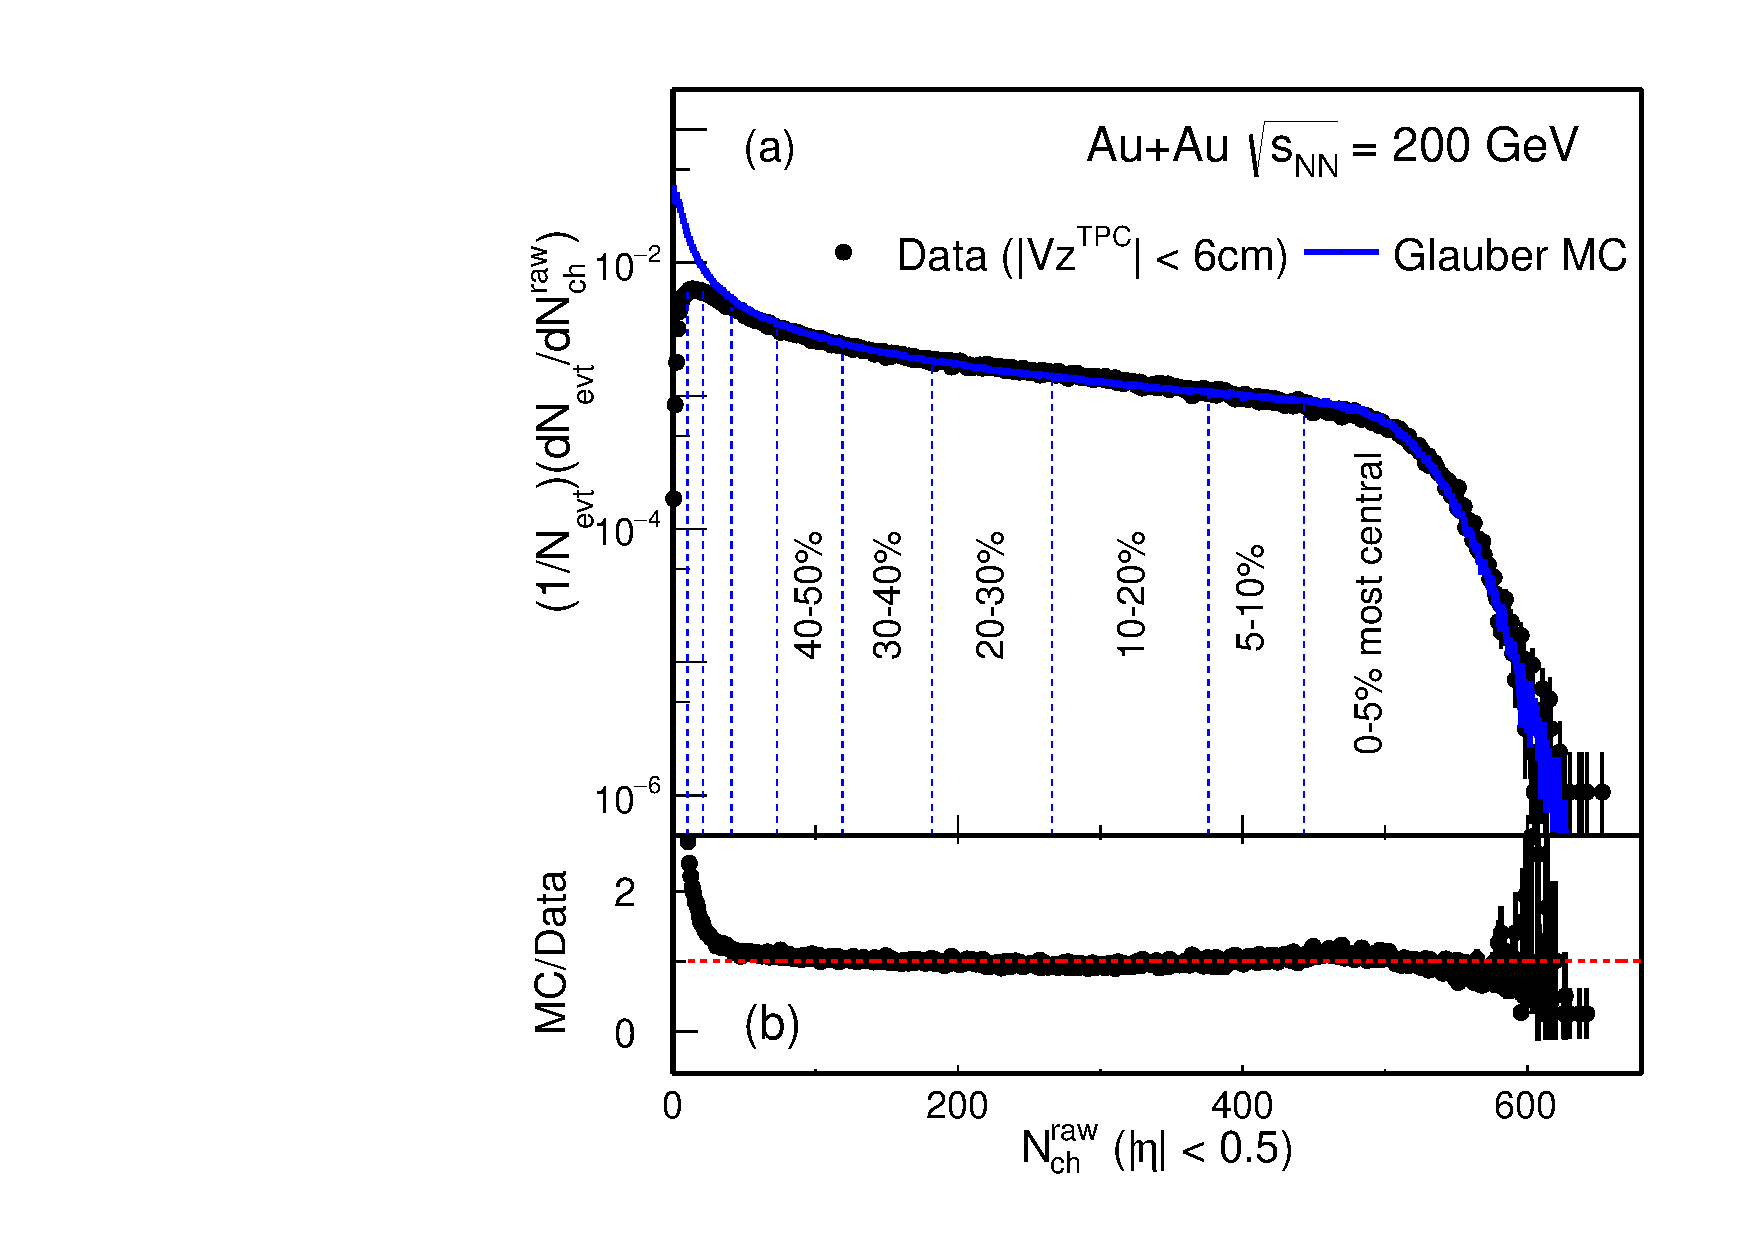
\includegraphics[width=0.45\textwidth]{fig/centrality.pdf}
  \caption{(a) Uncorrected charged particle multiplicity $N_{\rm ch}^{\rm raw}$ distribution measured with $|\eta|$ $<$ 0.5 and \DIFdelbeginFL \DIFdelFL{$|Vz|$ }\DIFdelendFL \DIFaddbeginFL \DIFaddFL{$|Vz^{\rm{TPC}}|$ }\DIFaddendFL $<$ 6 cm. The solid curve depicts the multiplicity distribution from a MC Glauber simulation fit to the experimental data. (b) Ratio between MC simulation and real data}
\label{fig:centrality} 
\end{figure}


\begin{figure*}
\centering
\DIFdelbeginFL %DIFDELCMD < 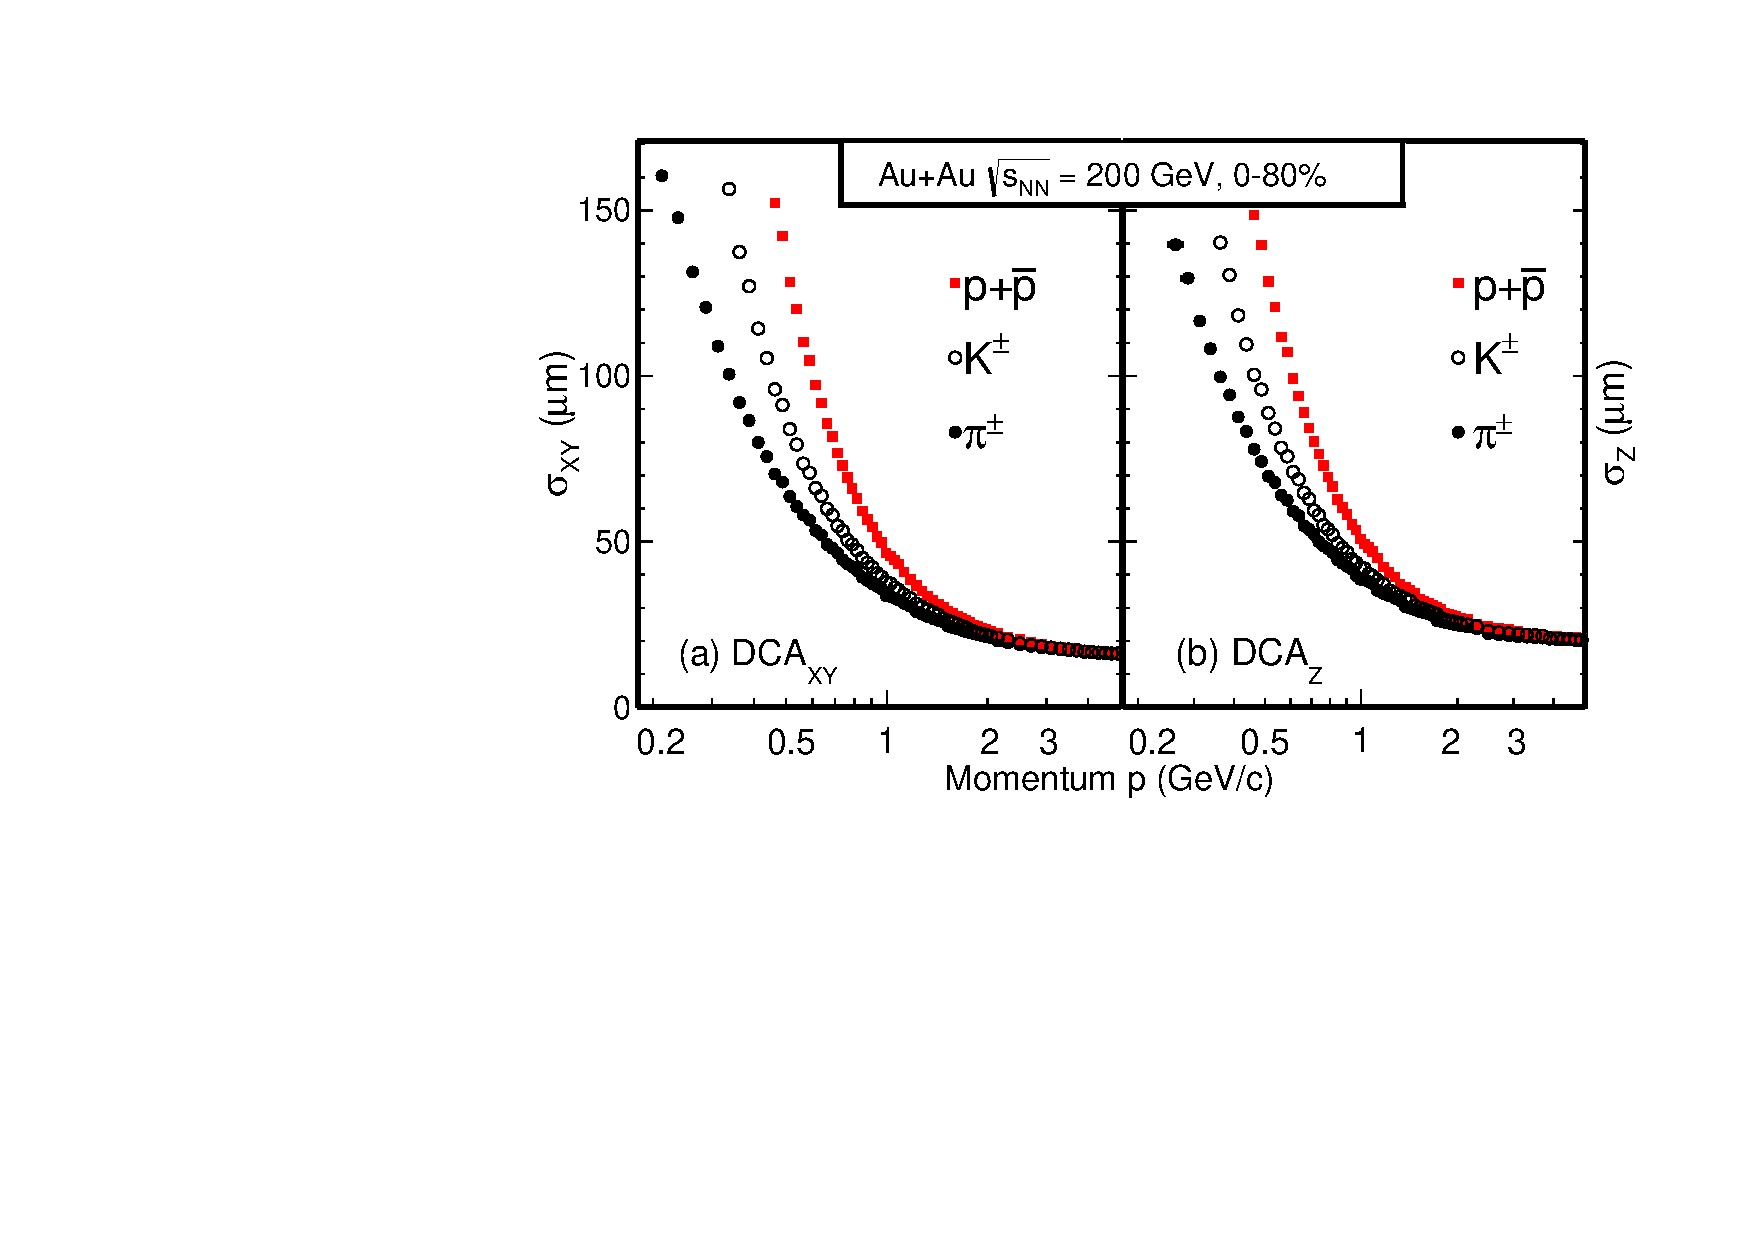
\includegraphics[width=0.85\textwidth]{fig/DCAXy_Z.pdf}
%DIFDELCMD < %%%
\DIFdelendFL \DIFaddbeginFL 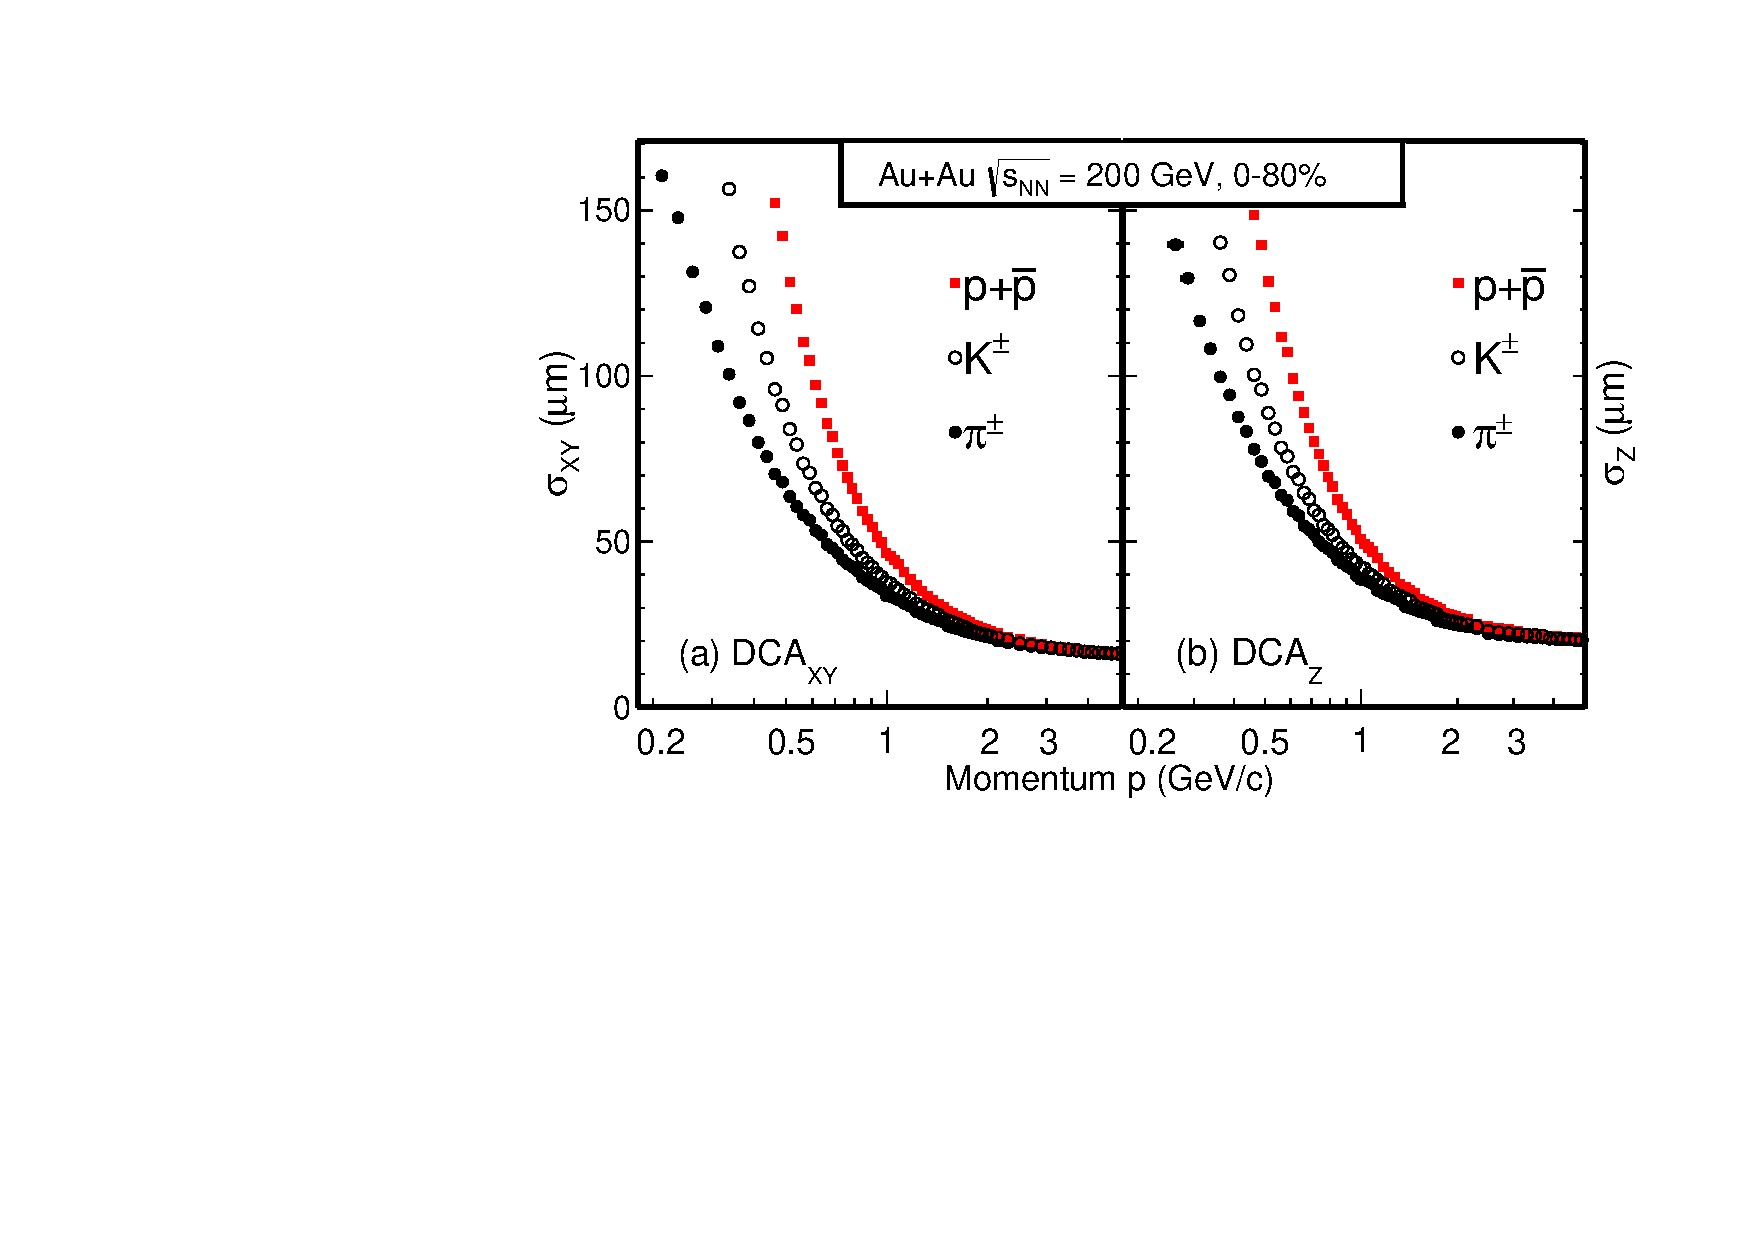
\includegraphics[width=0.78\textwidth]{fig/DCAXy_Z.pdf}
\DIFaddendFL \caption{Identified particle ($\pi^{\pm}$, $K^{\pm}$, and $p$+$\bar{p}$) pointing resolution in the transverse (a) and longitudinal (b) planes as a function of particle total momentum in Au+Au 0--80\% collisions\DIFdelbeginFL \DIFdelFL{at $\sqrt{s_{_{\rm NN}}}$ = 200\,GeV}\DIFdelendFL .}
\label{fig:DCAXy_Z} 
\end{figure*}

\begin{figure}[h]
\centering
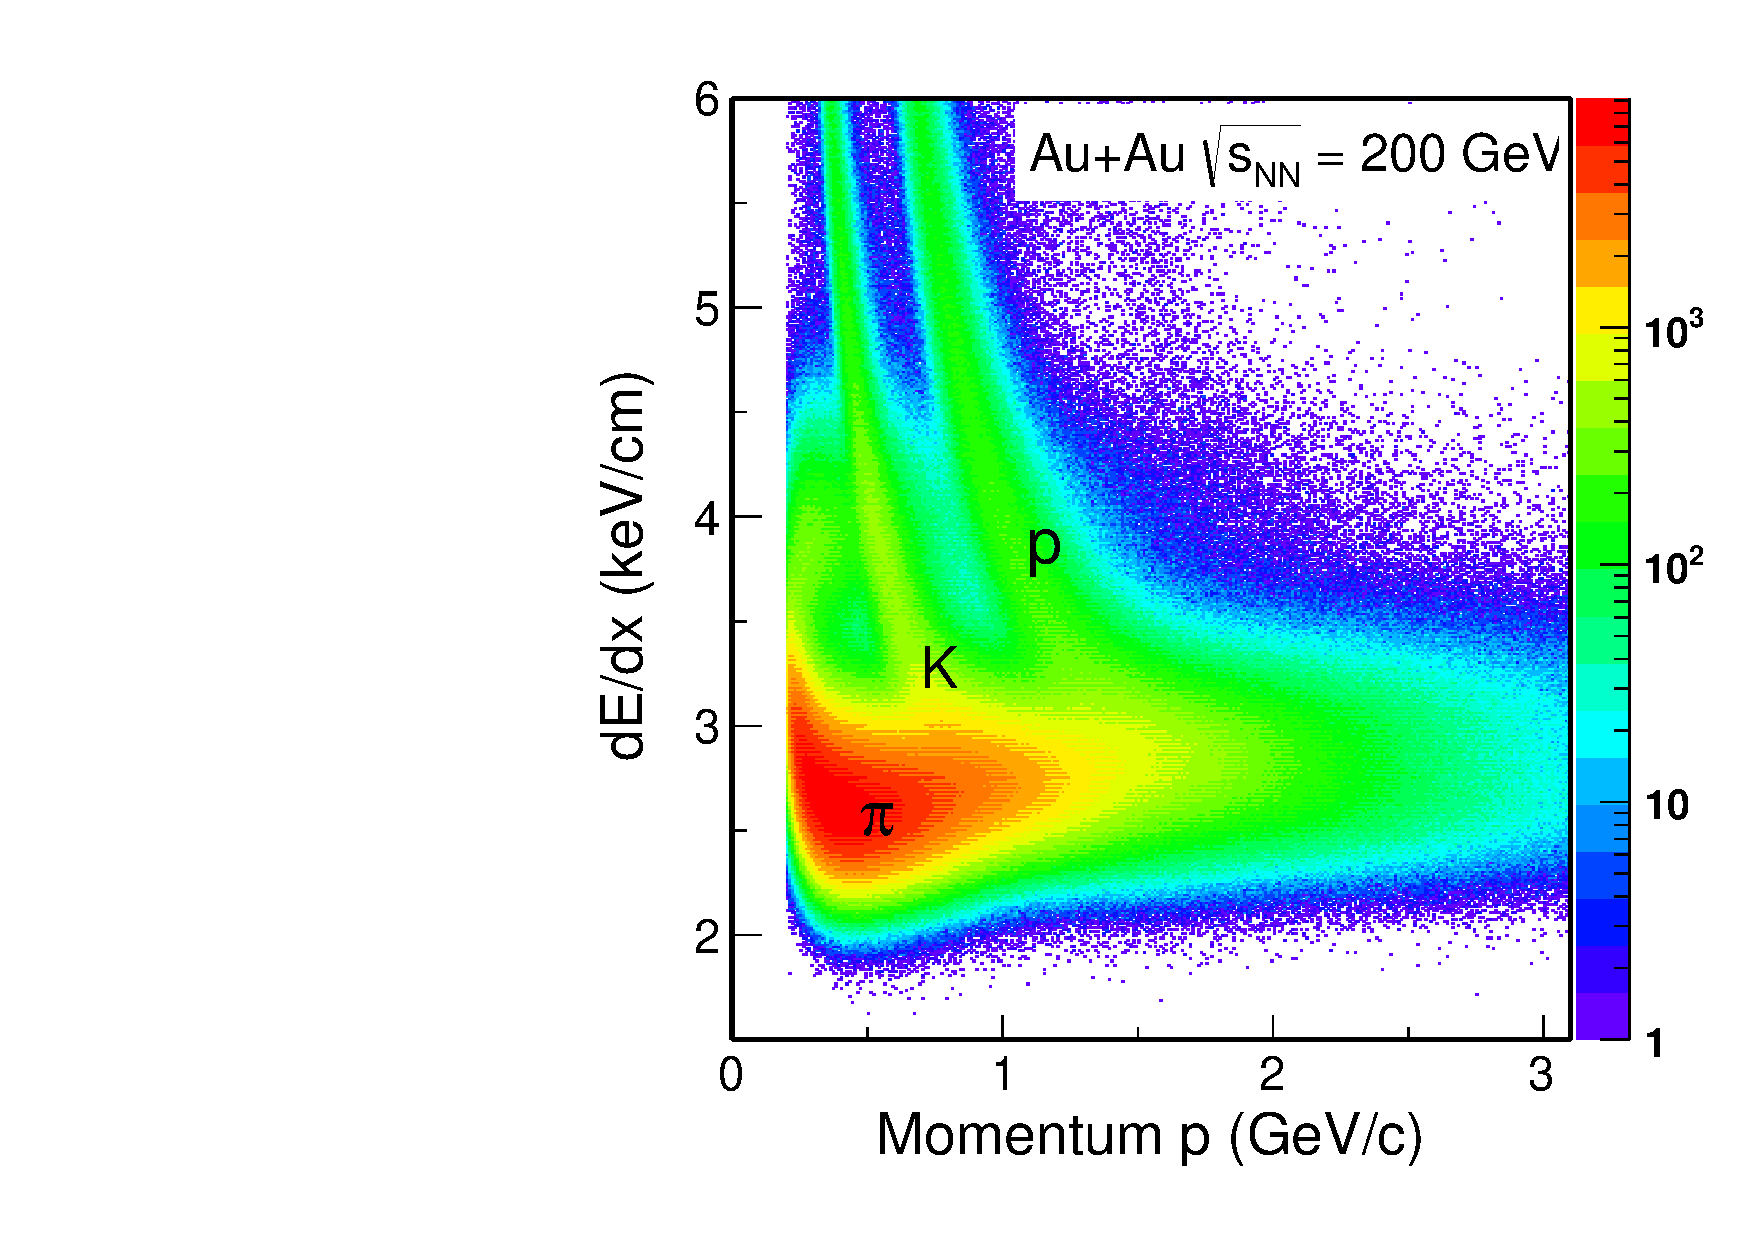
\includegraphics[width=0.45\textwidth]{fig/PID_dEdx.pdf}
\caption{TPC $dE/dx$ vs. particle momentum\DIFdelbeginFL \DIFdelFL{in Au + Au collisions at $\sqrt{s_{_{\rm NN}}}$ = 200\,GeV}\DIFdelendFL .}
\label{fig:PID_dEdx} 
\end{figure}

\begin{figure}[h]
\centering
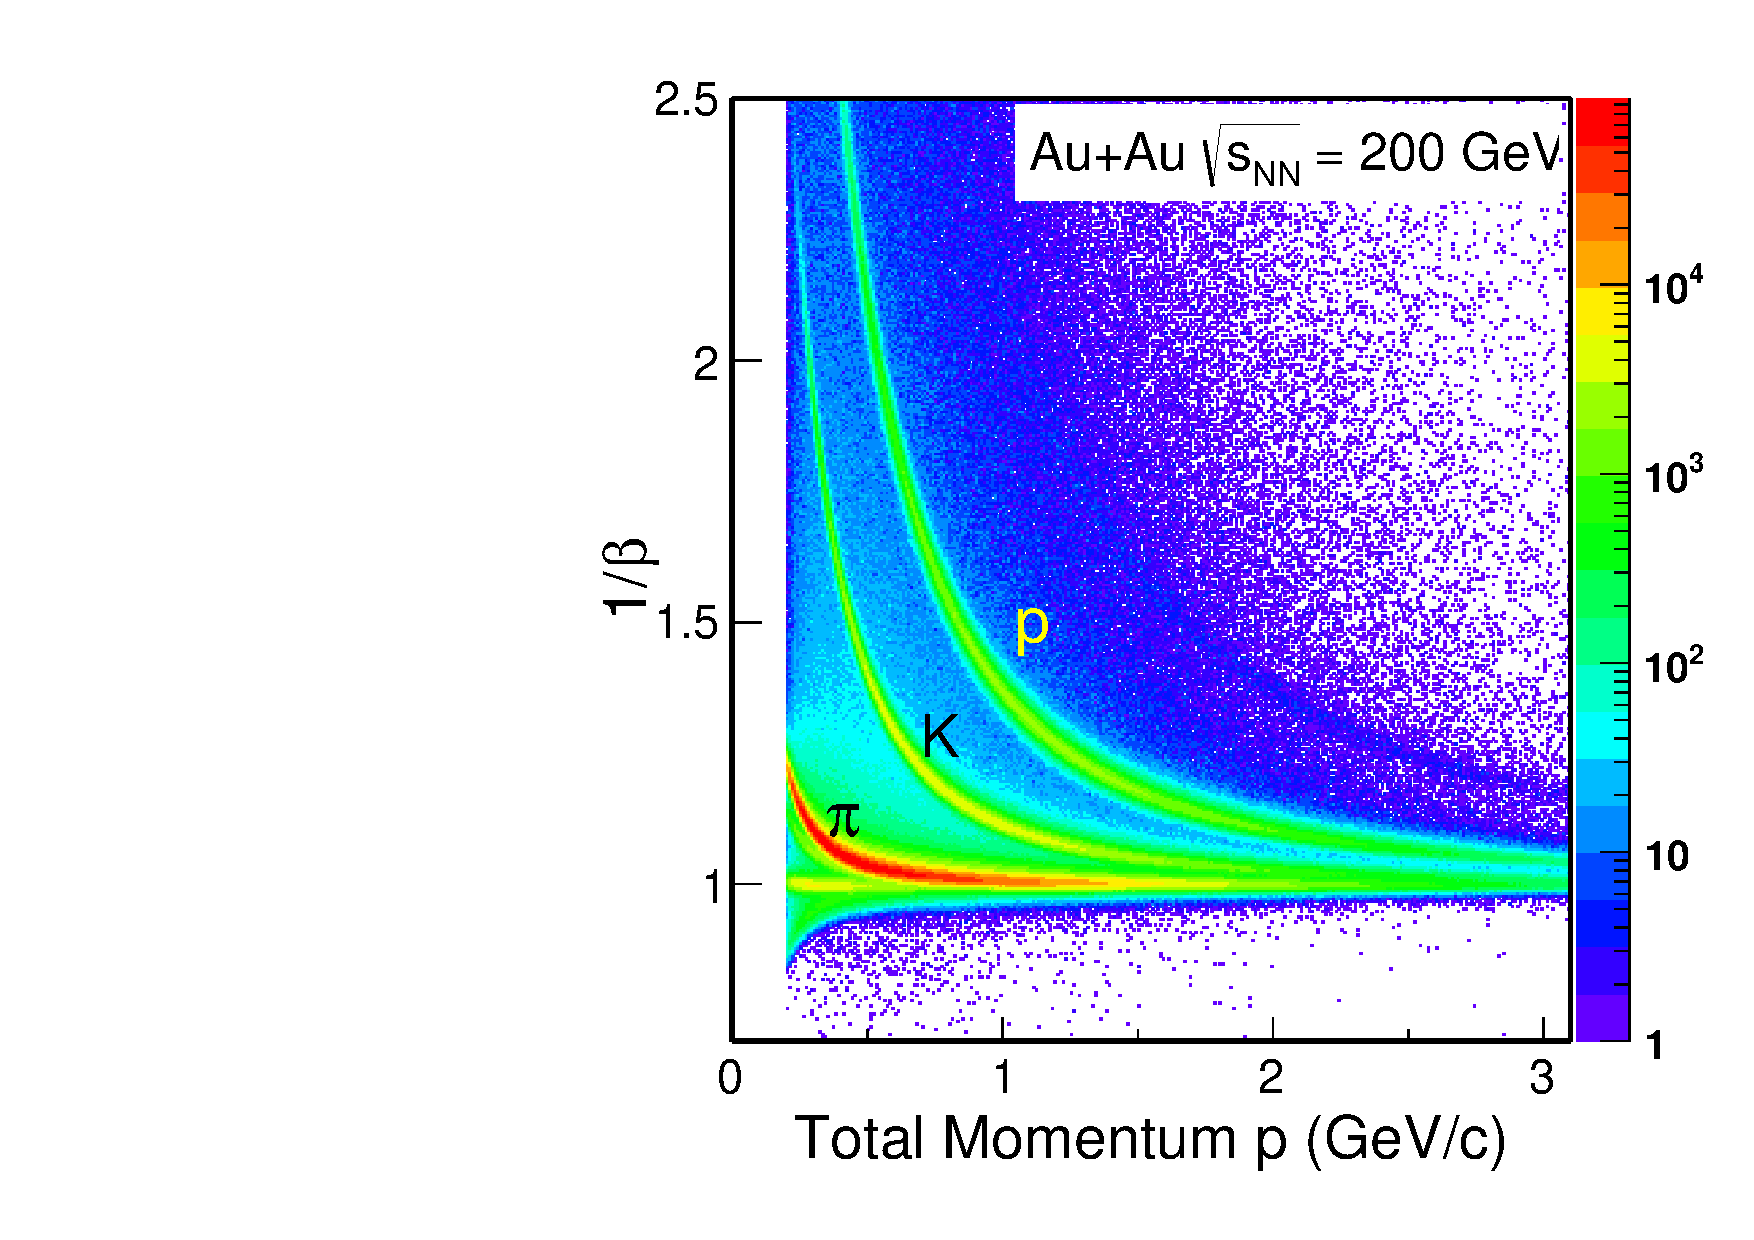
\includegraphics[width=0.45\textwidth]{fig/PID_beta.pdf}
\caption{TOF $1/\beta$ vs. particle momentum\DIFdelbeginFL \DIFdelFL{in Au + Au collisions at $\sqrt{s_{_{\rm NN}}}$ = 200\,GeV}\DIFdelendFL .}
\label{fig:PID_beta} 
\end{figure}

%DIF <  Table~\ref{table:ccentrality} 
\DIFdelbegin \DIFdel{TableI }\DIFdelend \DIFaddbegin \DIFadd{Table~\ref{table:ccentrality} }\DIFaddend lists the extracted values of number of binary collisions ($N_{\rm bin}$), number of participants ($N_{\rm part}$) and trigger inefficiency correction factors ($\varepsilon_{\rm trg}$) as well as their uncertainties. The $\varepsilon_{\rm trg}$ factors are \DIFaddbegin \DIFadd{the }\DIFaddend average values over in each centrality bins\DIFdelbegin \DIFdel{, while in }\DIFdelend \DIFaddbegin \DIFadd{. In }\DIFaddend practice we apply this correction factor event-by-event according to the measured $N_{\rm ch}^{\rm raw}$ \DIFdelbegin \DIFdel{of the }\DIFdelend \DIFaddbegin \DIFadd{for each }\DIFaddend event.

\begin{table*}[t]
\DIFdelbeginFL %DIFDELCMD < \centering{
%DIFDELCMD <   \caption{Estimated values of number of binary collisions ($N_{\rm bin}$), number of participants ($N_{\rm part}$) and trigger correction factors ($\varepsilon_{\rm trg}$, uncertainties negligible) for various centrality bins obtained from the MC Glauber model fit to the measured multiplicity distributions.}
%DIFDELCMD < \begin{tabular}{rcccccccc} \hline \hline
%DIFDELCMD < \hspace{1cm}Centrality\hspace{1cm} & \multicolumn{3}{c}{$N_{\rm bin}$} & \hspace{1cm} & \multicolumn{3}{c}{$N_{\rm part}$} & \hspace{1cm}$\varepsilon_{\rm trg}$\hspace{1cm} \\ \hline
%DIFDELCMD < 0--10 \%\hspace{1cm}      & 938.8 & $\pm$ & 26.3 & & 319.4 & $\pm$ & 3.4  & 1.0 \\
%DIFDELCMD < 10--20 \%\hspace{1cm}     & 579.9 & $\pm$ & 28.8 & & 227.6 & $\pm$ & 7.9  & 1.0 \\
%DIFDELCMD < 20--40 \%\hspace{1cm}     & 288.3 & $\pm$ & 30.4 & & 137.6 & $\pm$ & 10.4 & 1.0 \\
%DIFDELCMD < 40--60 \%\hspace{1cm}     & 91.3  & $\pm$ & 21.0 & & 60.5  & $\pm$ & 10.1 & 0.92 \\
%DIFDELCMD < 60--80 \%\hspace{1cm}     & 21.3  & $\pm$ & 8.9  & & 20.4  & $\pm$ & 6.6  & 0.65 \\ \hline \hline
%DIFDELCMD < \end{tabular}
%DIFDELCMD < }
%DIFDELCMD < %DIFDELCMD < \label{table:ccentrality}%%%
%DIFDELCMD < %%%
\DIFdelendFL \DIFaddbeginFL \centering{
\caption{Estimated values of number of binary collisions ($N_{\rm bin}$), number of participants ($N_{\rm part}$) and trigger correction factors ($\varepsilon_{\rm trg}$, uncertainties negligible) for various centrality bins obtained from the MC Glauber model fit to the measured multiplicity distributions.}
\begin{tabular}{rcccccccc} \hline \hline
\hspace{1cm}Centrality\hspace{1cm} & \multicolumn{3}{c}{$N_{\rm bin}$} & \hspace{1cm} & \multicolumn{3}{c}{$N_{\rm part}$} & \hspace{1cm}$\varepsilon_{\rm trg}$\hspace{1cm} \\ \hline
0--10 \%\hspace{1cm}      & 938.8 & $\pm$ & 26.3 & & 319.4 & $\pm$ & 3.4  & 1.0 \\
10--20 \%\hspace{1cm}     & 579.9 & $\pm$ & 28.8 & & 227.6 & $\pm$ & 7.9  & 1.0 \\
20--40 \%\hspace{1cm}     & 288.3 & $\pm$ & 30.4 & & 137.6 & $\pm$ & 10.4 & 1.0 \\
40--60 \%\hspace{1cm}     & 91.3  & $\pm$ & 21.0 & & 60.5  & $\pm$ & 10.1 & 0.92 \\
60--80 \%\hspace{1cm}     & 21.3  & $\pm$ & 8.9  & & 20.4  & $\pm$ & 6.6  & 0.65 \\ \hline \hline
\end{tabular}
\label{table:ccentrality}
}
\DIFaddendFL \end{table*}

\subsection{\DIFdelbegin %DIFDELCMD < %DIFDELCMD < \label{sec:dataset:hft}%%%
%%%
\DIFdelend Heavy Flavor Tracker}
\DIFaddbegin \label{dataset:hft}

\DIFaddend The HFT~\cite{HFTQM14} is a high resolution silicon detector system, that aims for the topological reconstruction of secondary decay vertices. It consists of three silicon subsystems: the Silicon Strip Detector (SSD), the Intermediate Silicon Tracker (IST), and \DIFdelbegin \DIFdel{the }\DIFdelend two layers of \DIFaddbegin \DIFadd{the }\DIFaddend PiXeL (PXL) detector. 
%DIF <  Table~\ref{table:HFT} 
\DIFdelbegin \DIFdel{TableII }\DIFdelend \DIFaddbegin \DIFadd{Table~\ref{table:HFT} }\DIFaddend lists the key characteristic parameters of each subsystem. The SSD detector \DIFdelbegin \DIFdel{is still in the commissioning stage }\DIFdelend \DIFaddbegin \DIFadd{was still under commission stage during }\DIFaddend when the dataset \DIFdelbegin \DIFdel{used in this analysis are taken}\DIFdelend \DIFaddbegin \DIFadd{was recorded}\DIFaddend , and therefore is not used in the offline data production and this analysis.
%They lay inside the TPC with incrementally improved resolution, SSD sit away from the beam with a radius $\sim$ 22 cm, IST around $\sim$ 14 cm and two layers of PXL with $\sim$ 8 cm and $\sim$ 2.8 cm respectively. 
The PXL detector uses the new Monolithic Active Pixel Sensors (MAPS) technology~\cite{PXL}. This is the first application of this technology in a collider experiment. It is particularly designed to measure heavy-flavor hadron decays in the high multiplicity heavy-ion collision environment.

%%% Need to confirm all the numbers
\begin{table*}[t]
\DIFdelbeginFL %DIFDELCMD < \centering{
%DIFDELCMD < \caption{Several key characteristic parameters for each subsystem of the HFT detector.}
%DIFDELCMD < \begin{tabular}{ccccc} \hline \hline
%DIFDELCMD < \hspace{0.5cm}Subsystem\hspace{0.5cm} & \hspace{0.5cm}Radii (cm)\hspace{0.5cm} & \hspace{0.5cm}Length (cm)\hspace{0.5cm} & \hspace{0.5cm}Thickness at $\eta=0$ ($X_{0}$)\hspace{0.5cm} & \hspace{0.5cm}Pitch Size ($\mu m^2$)\hspace{0.5cm} \\ \hline
%DIFDELCMD < PXL inner layer & 2.8 & 20 & 0.52\% (0.39\%$^{\dagger}$) & 20.7$\times$20.7 \\
%DIFDELCMD < PXL outer layer & 8.0 & 20 & 0.52\% & 20.7$\times$20.7 \\
%DIFDELCMD < IST & 14.0 & 50 & 1.0\% & 600$\times$6000 \\
%DIFDELCMD < SSD$^{\dagger\dagger}$ & 22.0 & 106 & 1.0\% & 95$\times$40000 \\ \hline \hline
%DIFDELCMD < \end{tabular} \\
%DIFDELCMD < $^{\dagger}$ - PXL inner detector material is reduced to 0.39\%$X_0$ in 2015/2016 runs. \\
%DIFDELCMD < $^{\dagger\dagger}$ - SSD is not included in this analysis.}
%DIFDELCMD < %DIFDELCMD < \label{table:HFT} %%%
%DIFDELCMD < %%%
\DIFdelendFL \DIFaddbeginFL \centering{
\caption{Several key characteristic parameters for each subsystem of the HFT detector.}
\begin{tabular}{ccccc} \hline \hline
  \hspace{0.5cm}Subsystem\hspace{0.5cm} & \hspace{0.5cm}Radius (cm)\hspace{0.5cm} & \hspace{0.5cm}Length (cm)\hspace{0.5cm} & \hspace{0.5cm}Thickness at $\eta=0$ ($X_{0}$)\hspace{0.5cm} & \hspace{0.5cm}Pitch Size ($\upmu \textup{m}^2$)\hspace{0.5cm} \\ \hline
PXL inner layer & 2.8 & 20 & 0.52\% (0.39\%$^{\dagger}$) & 20.7$\times$20.7 \\
PXL outer layer & 8.0 & 20 & 0.52\% & 20.7$\times$20.7 \\
IST & 14.0 & 50 & 1.0\% & 600$\times$6000 \\
SSD$^{\dagger\dagger}$ & 22.0 & 106 & 1.0\% & 95$\times$40000 \\ \hline \hline
\end{tabular} \\
$^{\dagger}$ - PXL inner detector material is reduced to 0.39\%$X_0$ in 2015/2016 runs. \\
$^{\dagger\dagger}$ - SSD is not included in this analysis.
\label{table:HFT} 
}
\DIFaddendFL \end{table*}
%DIF <  The HFT participated in the full 2014 Au + Au 200GeV runs in STAR.
%DIF >  The HFT participated in the full 2014 Au+Au 200GeV runs in STAR.

In the offline reconstruction, tracks are reconstructed in the TPC first and then extended to the HFT detector to find the best fit to the measured high resolution \DIFdelbegin \DIFdel{spacial }\DIFdelend \DIFaddbegin \DIFadd{spatial }\DIFaddend points. The tracking algorithm with \DIFaddbegin \DIFadd{the }\DIFaddend Kalman filter that considers various detector material effects is used in the track extension. Considering the background hits level \DIFdelbegin \DIFdel{at }\DIFdelend \DIFaddbegin \DIFadd{in }\DIFaddend the PXL due to pileup hadronic and electromagnetic collisions, tracks are required to have at least one hit in each layer of \DIFaddbegin \DIFadd{the }\DIFaddend IST and PXL subdetectors. \DIFdelbegin \DIFdel{Fig.}\DIFdelend \DIFaddbegin \DIFadd{Figure}\DIFaddend ~\ref{fig:DCAXy_Z} shows the track pointing resolution to the primary vertex in the transverse plane ($\sigma_{\rm XY}$) in panel (a) and along the longitudinal direction ($\sigma_{\rm Z}$) in panel (b) as a function of momentum ($p$) for identified particles in \DIFdelbegin \DIFdel{0-80\% }\DIFdelend \DIFaddbegin \DIFadd{$\rm{0-80\%}$ }\DIFaddend centrality Au+Au collisions\DIFdelbegin \DIFdel{at $\sqrt{s_{\rm NN}}$ = 200\,GeV}\DIFdelend . The design goal for the HFT detector \DIFdelbegin \DIFdel{is }\DIFdelend \DIFaddbegin \DIFadd{was }\DIFaddend to have a pointing resolution better than 55 \DIFdelbegin \DIFdel{$\mu m$ }\DIFdelend \DIFaddbegin \DIFadd{$\upmu$m }\DIFaddend for 750\,MeV Kaons. \DIFdelbegin \DIFdel{Fig.}\DIFdelend \DIFaddbegin \DIFadd{Figure}\DIFaddend ~\ref{fig:DCAXy_Z} demonstrates that the HFT detector system \DIFdelbegin \DIFdel{has delivered a performance that satisfies the requirements for open heavy flavor physics measurements. }\DIFdelend \DIFaddbegin \DIFadd{meets the design requirements. This performance enabled the study of the D-meson production with a high significance signal.
}\DIFaddend 


% Chapter three
\section{\DIFdelbegin %DIFDELCMD < %DIFDELCMD < \label{sec:D0recon}%%%
%%%
\DIFdelend $D^0$-meson reconstruction}
\DIFaddbegin \label{D0recon}
\DIFaddend 

$D^0$ and $\overline{D}^{0}$ mesons are reconstructed via the hadronic decay channel $D^0\rightarrow K^-+\pi^+$ and its charge conjugate channel with a branching ratio of 3.89\%. In what follows, we imply $(D^0 +\overline{D}^{0})/2$ when using the term $D^0$ unless otherwise specified. $D^0$ mesons decay with a proper decay length of \DIFdelbegin \DIFdel{$c\tau\sim123\ \mu$}\DIFdelend \DIFaddbegin \DIFadd{$c\tau\sim123\ \upmu$}\DIFaddend m after they are produced in Au+Au collisions. We utilize the \DIFdelbegin \DIFdel{high pointing }\DIFdelend \DIFaddbegin \DIFadd{high-pointing }\DIFaddend resolution capability enabled by the HFT detector to topologically reconstruct the $D^0$ decay vertices that are separated from the collision vertices, which drastically reduces \DIFaddbegin \DIFadd{($\sim$5 order of magnitude) }\DIFaddend the combinational background and improves the measurement precision.

Charged pion and kaon tracks are reconstructed with the TPC and the HFT. Tracks are required to have at least 20 measured TPC points out of maximum 45 to ensure \DIFdelbegin \DIFdel{good momentum measurement}\DIFdelend \DIFaddbegin \DIFadd{with good momentum resolution}\DIFaddend . To enable high pointing precision, both daughter tracks are required to have at least one measured hit in each layer of PXL and IST as described above. Particle identification is achieved via a combination of the ionization energy loss \DIFdelbegin \DIFdel{($dE/dx$) }\DIFdelend measurement in the TPC and the \DIFdelbegin \DIFdel{$tof$ }\DIFdelend \DIFaddbegin \DIFadd{tof }\DIFaddend measurement in the TOF. The resolution-normalized $dE/dx$ deviation from the expected values is defined as:
\DIFdelbegin \[
%DIF <  N\sigma_X = \frac{dE/dx_{mea}-dE/dx_{th}}{R}
\DIFdel{n\sigma_X = \frac{1}{R}\ln\frac{\langle{dE/dx}\rangle_{mea.}}{\langle{dE/dx}\rangle_{X}}
}\]
%DIFAUXCMD
\DIFdel{Where }\DIFdelend \DIFaddbegin \begin{equation}
%DIF >  \[
%DIF >  N\sigma_X = \frac{dE/dx_{mea}-dE/dx_{th}}{R}
\DIFadd{n\sigma_X = \frac{1}{R}\ln\frac{\langle{dE/dx}\rangle_{mea.}}{\langle{dE/dx}\rangle_{X}},
}\end{equation}
\label{equ:equation1}
\]
\DIFadd{where }\DIFaddend $\langle{dE/dx}\rangle_{mea.}$ and $\langle{dE/dx}\rangle_{X}$ represent measured and \DIFdelbegin \DIFdel{theoretical }\DIFdelend \DIFaddbegin \DIFadd{expected }\DIFaddend $dE/dx$, and $R$ is the STAR TPC $dE/dx$ resolution (typically $\sim$8\%\DIFaddbegin \DIFadd{~\mbox{%DIFAUXCMD
\cite{TPC}}%DIFAUXCMD
}\DIFaddend ). The $n\sigma_X$ should be close to a standard Gaussian distribution for each corresponding particle species (mean $=$ 0, $\sigma = $ 1).
Pion (kaon) candidates are selected by a requirement of the measured $dE/dx$ to be within three (two) standard \DIFdelbegin \DIFdel{deviation }\DIFdelend \DIFaddbegin \DIFadd{deviations }\DIFaddend ($|n\sigma_{X}|$) from the expected \DIFdelbegin \DIFdel{values}\DIFdelend \DIFaddbegin \DIFadd{value}\DIFaddend . When tracks have matched hits in the TOF detector, an additional requirement on the measured \DIFaddbegin \DIFadd{inverse }\DIFaddend particle velocity (\DIFdelbegin \DIFdel{$\beta$}\DIFdelend \DIFaddbegin \DIFadd{$1/\beta$}\DIFaddend ) to be within three standard \DIFdelbegin \DIFdel{deviation }\DIFdelend \DIFaddbegin \DIFadd{deviations }\DIFaddend from the expected \DIFdelbegin \DIFdel{values }\DIFdelend \DIFaddbegin \DIFadd{value }\DIFaddend ($|\Delta 1/\beta|$) is applied for either daughter track. \DIFdelbegin \DIFdel{Fig}\DIFdelend \DIFaddbegin \DIFadd{Figures}\DIFaddend .~\ref{fig:PID_dEdx} and \DIFdelbegin \DIFdel{Fig.}\DIFdelend ~\ref{fig:PID_beta} show an example of the particle identification capability from TPC and TOF. Tracks within the kinematic acceptance \DIFdelbegin \DIFdel{$p_{\rm T}>0.6$ }\DIFdelend \DIFaddbegin \DIFadd{$p_{T}>0.6$ }\DIFaddend GeV/$c$ and $|\eta|<1$ \DIFdelbegin \DIFdel{) }\DIFdelend are used to combine and make pairs. Table~\ref{table:singlecut} lists the TPC and TOF selection cuts for daughter kaon and pion tracks used for $D^0$ reconstruction.

\begin{table}
\DIFdelbeginFL %DIFDELCMD < \centering{
%DIFDELCMD < \caption{TPC and TOF selection cuts for $K$ and $\pi$ tracks.}
%DIFDELCMD < \begin{tabular}{cccc} \hline \hline
%DIFDELCMD < Variable & & $K^{\mp}$  & $\pi^{\pm}$ \\ \hline
%DIFDELCMD < $p_{\rm T}$ (GeV/$c$)   & $>$ & 0.6 & 0.6 \\
%DIFDELCMD < $|\eta|$			    & $<$ & 1.0 & 1.0 \\
%DIFDELCMD < nHitsFit (TPC)		    & $>$ & 20  & 20 \\
%DIFDELCMD < % nHitsFit/nHitsMax (TPC) & $>$ & 0.52 & 0.52 \\
%DIFDELCMD < $|n\sigma_{X}|$         & $<$ & 2.0 & 3.0 \\
%DIFDELCMD < $|\Delta 1/\beta|$ (if $\beta>0$)     & $<$ & 0.03 & 0.03 \\ \hline \hline
%DIFDELCMD < \end{tabular}
%DIFDELCMD < }
%DIFDELCMD < %%%
\DIFdelendFL \DIFaddbeginFL \centering{
\caption{TPC and TOF selection cuts for $K$ and $\pi$ tracks.}
\begin{tabular}{cccc} \hline \hline
Variable & & $K^{\mp}$  & $\pi^{\pm}$ \\ \hline
$p_{T}$ (GeV/$c$)   & $>$ & 0.6 & 0.6 \\
$|\eta|$			    & $<$ & 1.0 & 1.0 \\
nHitsFit (TPC)		    & $>$ & 20  & 20 \\
% nHitsFit/nHitsMax (TPC) & $>$ & 0.52 & 0.52 \\
$|n\sigma_{X}|$         & $<$ & 2.0 & 3.0 \\
$|\Delta 1/\beta|$ (if TOF matched)     & $<$ & 0.03 & 0.03 \\ \hline \hline
\end{tabular}
}
\DIFaddendFL \label{table:singlecut} 
\end{table}

\begin{figure*}
\centering
\DIFdelbeginFL %DIFDELCMD < 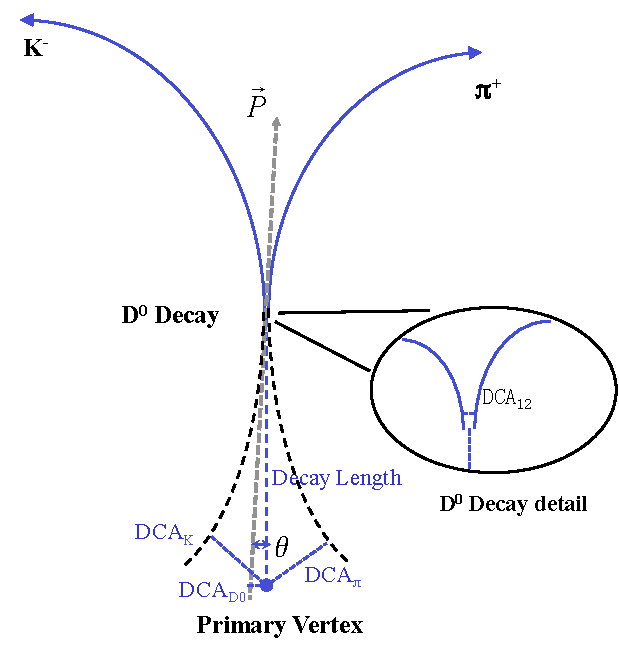
\includegraphics[width=0.6\textwidth]{fig/D0carton.pdf}
%DIFDELCMD < %%%
\DIFdelendFL \DIFaddbeginFL 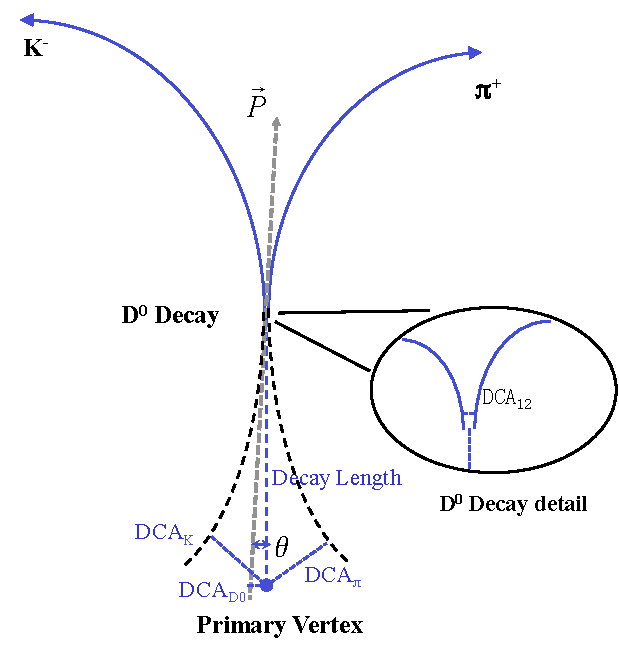
\includegraphics[width=0.50\textwidth]{fig/D0carton.pdf}
\DIFaddendFL \caption{$D^{0}$ topological variables used in the reconstruction.}
\label{fig:D0carton} 
\end{figure*}

With a pair of two daughter tracks, pion and kaon, the $D^0$ decay vertex is reconstructed as the middle point on the distance of the \DIFdelbegin \DIFdel{closet }\DIFdelend \DIFaddbegin \DIFadd{closest }\DIFaddend approach between the two daughter trajectories. The background is mainly due to the random combination of the fake pairs directly from the collision point. With the following topological variables, the background can be greatly reduced.

 \begin{itemize} 
  \item Decay Length: the distance between the reconstructed decay vertex and the \DIFdelbegin \DIFdel{primary vertex (PV}\DIFdelend \DIFaddbegin \DIFadd{Primary Vertex (PV, $V_{z}^{\rm TPC}$}\DIFaddend ).
  \item Distance of Closest Approach (DCA) between the 2 daughter tracks \DIFdelbegin \DIFdel{. ($\rm DCA_{12}$)}\DIFdelend \DIFaddbegin \DIFadd{($\rm{DCA_{12}}$).
  }\DIFaddend \item DCA between \DIFaddbegin \DIFadd{the }\DIFaddend reconstructed $D^0$ and the PV \DIFdelbegin \DIFdel{. ($\rm DCA_{D^{0}}$)}\DIFdelend \DIFaddbegin \DIFadd{($\rm{DCA_{D^{0}}}$).
  }\DIFaddend \item DCA between the pion and the PV \DIFdelbegin \DIFdel{. ($\rm DCA_{\pi}$)}\DIFdelend \DIFaddbegin \DIFadd{($\rm{DCA_{\pi}}$).
  }\DIFaddend \item DCA between the kaon and the PV \DIFdelbegin \DIFdel{. ($\rm DCA_{K}$)}\DIFdelend \DIFaddbegin \DIFadd{($\rm{DCA_{K}}$).
  }\DIFaddend \item Angle between $D^0$ momentum and the line between the reconstructed decay vertex and the PV \DIFdelbegin \DIFdel{. }\DIFdelend ($\theta$)\DIFaddbegin \DIFadd{.
}\DIFaddend  \end{itemize} 

The \DIFdelbegin \DIFdel{carton }\DIFdelend \DIFaddbegin \DIFadd{schematic in }\DIFaddend Fig.~\ref{fig:D0carton} also shows the topological variables used in the analysis, where $\vec{P}$ represent the $D^0$ momentum. The Decay Length and \DIFdelbegin \DIFdel{cos(}\DIFdelend \DIFaddbegin \DIFadd{angle }\DIFaddend $\theta$ \DIFdelbegin \DIFdel{) }\DIFdelend follow the formula: $\rm DCA_{D^{0}}$ = Decay Length $\times$ sin($\theta$). The cuts on the topological variables for this analysis are optimized using a Toolkit for Multivariate Data Analysis (TMVA) package\DIFaddbegin \DIFadd{~\mbox{%DIFAUXCMD
\cite{TMVA}}%DIFAUXCMD
, which developed from CERN, }\DIFaddend in order to have the greatest signal significance. We explored several different discrimination methods in the TMVA package and the Rectangular cut \DIFdelbegin \DIFdel{optimisation }\DIFdelend \DIFaddbegin \DIFadd{Optimization }\DIFaddend method is chosen for \DIFdelbegin \DIFdel{best signal }\DIFdelend significance estimation. The optimization is conducted for different $D^0$ \DIFdelbegin \DIFdel{$p_{\rm T}$ bins and difference }\DIFdelend \DIFaddbegin \DIFadd{$p_{T}$ bins and different }\DIFaddend centrality bins. Table~\ref{table:topocut} lists a typical set of topological cuts for 0-10\% central Au+Au collisions.

\begin{table*}[t]
\centering {
\caption{$D^0$ topological cuts for the 0-10\% most central collisions in \DIFdelbeginFL \DIFdelFL{separated }\DIFdelendFL \DIFaddbeginFL \DIFaddFL{separate }\DIFaddendFL $p_T$ ranges.}
\begin{tabular}{cc|ccccccc} \hline \hline
\DIFdelbeginFL \DIFdelFL{$0-10\% \ |\ p_{\rm T}$ }\DIFdelendFL \DIFaddbeginFL \DIFaddFL{$0-10\% \ |\ p_{T}$ }\DIFaddendFL (GeV/$c$) &    & \hspace{0.5cm}(0,0.5)\hspace{0.5cm} & \hspace{0.5cm}(0.5,1)\hspace{0.5cm} & \hspace{0.5cm}(1,2)\hspace{0.5cm} & \hspace{0.5cm}(2,3)\hspace{0.5cm} & \hspace{0.5cm}(3,5)\hspace{0.5cm} &  \hspace{0.5cm}(5,8)\hspace{0.5cm} &  \hspace{0.5cm}(8,10)\hspace{0.5cm} \\ \hline
  Decay Length (\DIFdelbeginFL \DIFdelFL{$\mu m$}\DIFdelendFL \DIFaddbeginFL \DIFaddFL{$\upmu$m}\DIFaddendFL ) & $>$ & 100 & 199 & 227 & 232 & 236 & 255 & 255 \\
  $\rm DCA_{12}$        (\DIFdelbeginFL \DIFdelFL{$\mu m$}\DIFdelendFL \DIFaddbeginFL \DIFaddFL{$\upmu$m}\DIFaddendFL ) & $<$ & 71  & 64 & 70 & 63 & 82 & 80 & 80 \\
  $\rm DCA_{D^{0}}$       (\DIFdelbeginFL \DIFdelFL{$\mu m$}\DIFdelendFL \DIFaddbeginFL \DIFaddFL{$\upmu$m}\DIFaddendFL ) & $<$ & 62  & 55 & 40 & 40 & 40 & 44 & 44 \\
  $\rm DCA_{\pi}$  (\DIFdelbeginFL \DIFdelFL{$\mu m$}\DIFdelendFL \DIFaddbeginFL \DIFaddFL{$\upmu$m}\DIFaddendFL ) & $>$ & 133 & 105 & 93 & 97 & 67 & 55 & 55 \\
  $\rm DCA_{K}$    (\DIFdelbeginFL \DIFdelFL{$\mu m$}\DIFdelendFL \DIFaddbeginFL \DIFaddFL{$\upmu$m}\DIFaddendFL ) & $>$ & 138 & 109 & 82 & 94 & 76 & 54 & 54 \\ 
  $\cos(\theta)$          & $>$ & 0.95 & 0.95 & 0.95 & 0.95 & 0.95 & 0.95 & 0.95 \\ \hline \hline
\end{tabular}
\label{table:topocut}
}
\end{table*}

\begin{figure*}
\centering
% 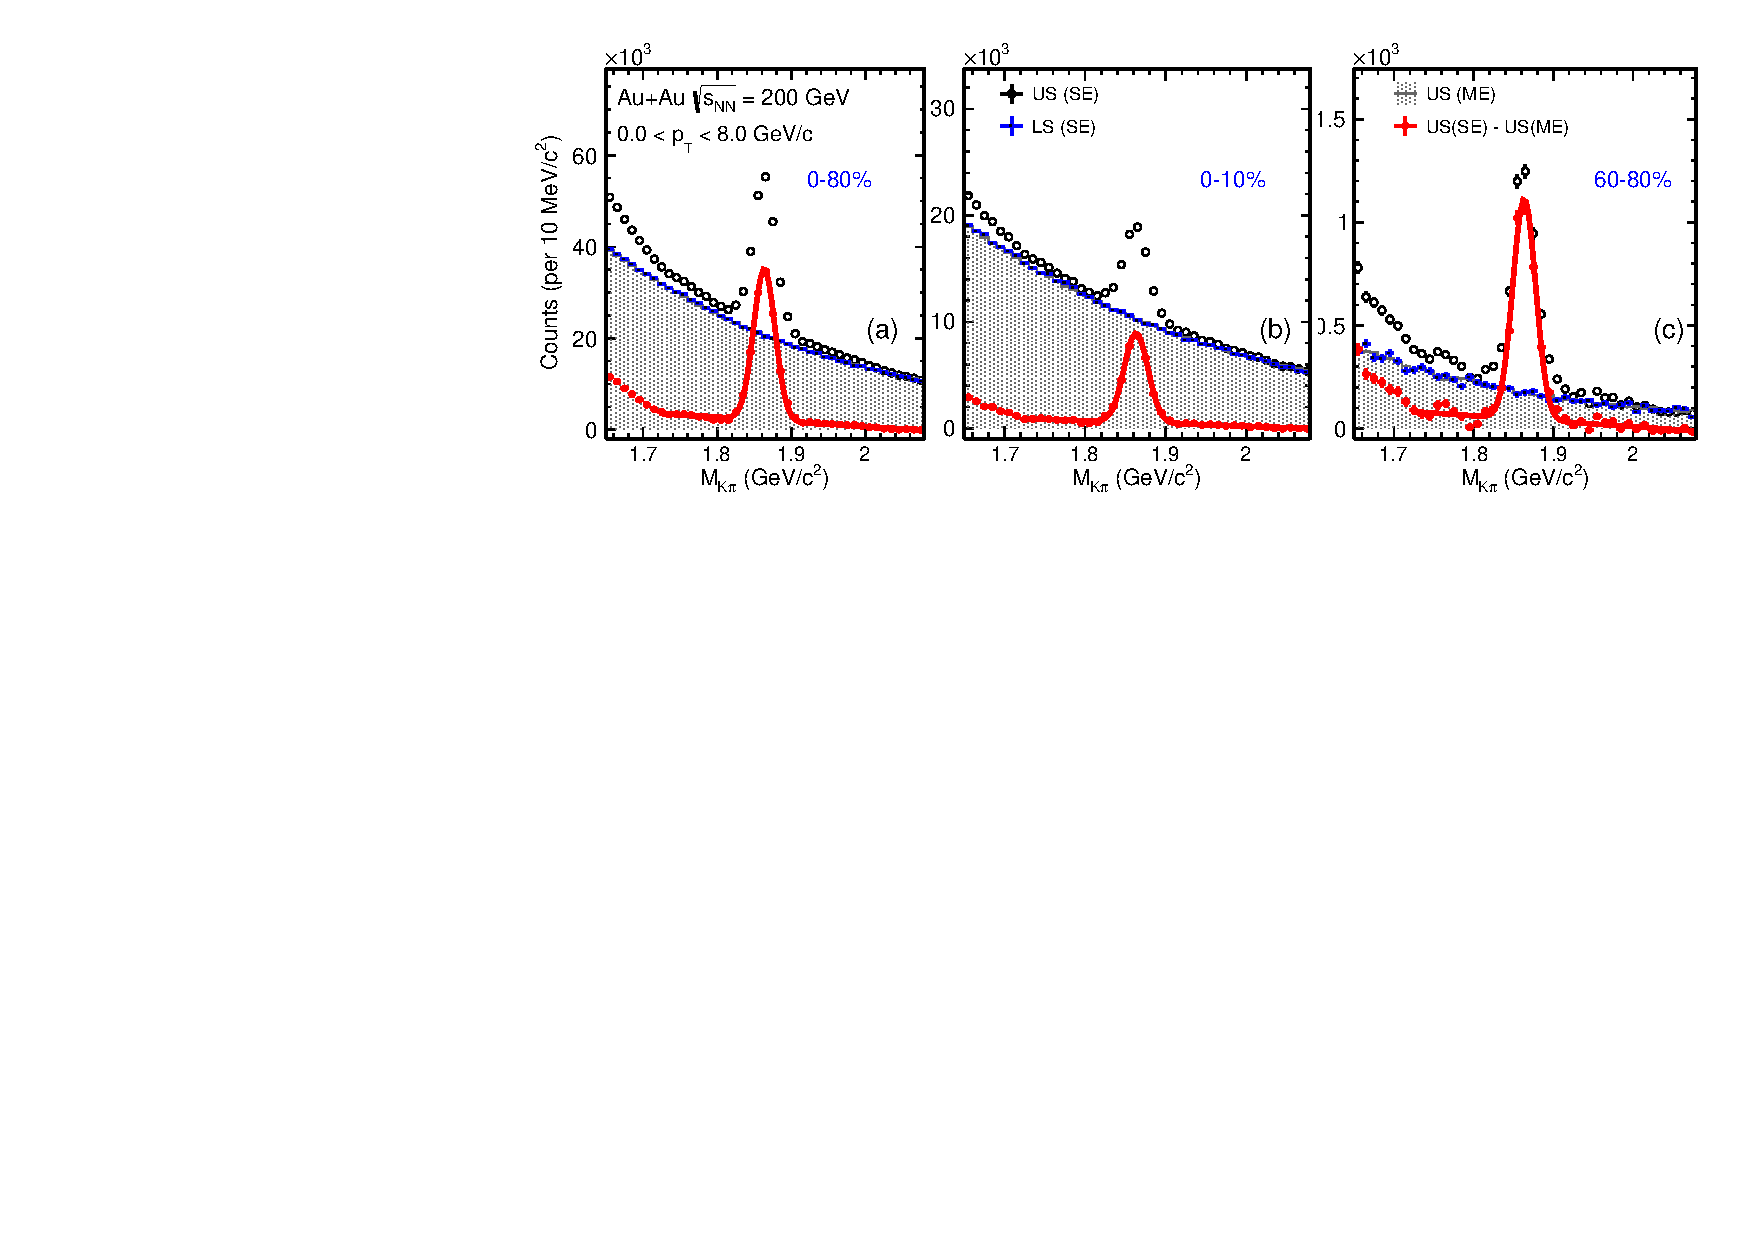
\includegraphics[width=1.0\textwidth]{fig/signal_0_8GeV.pdf}
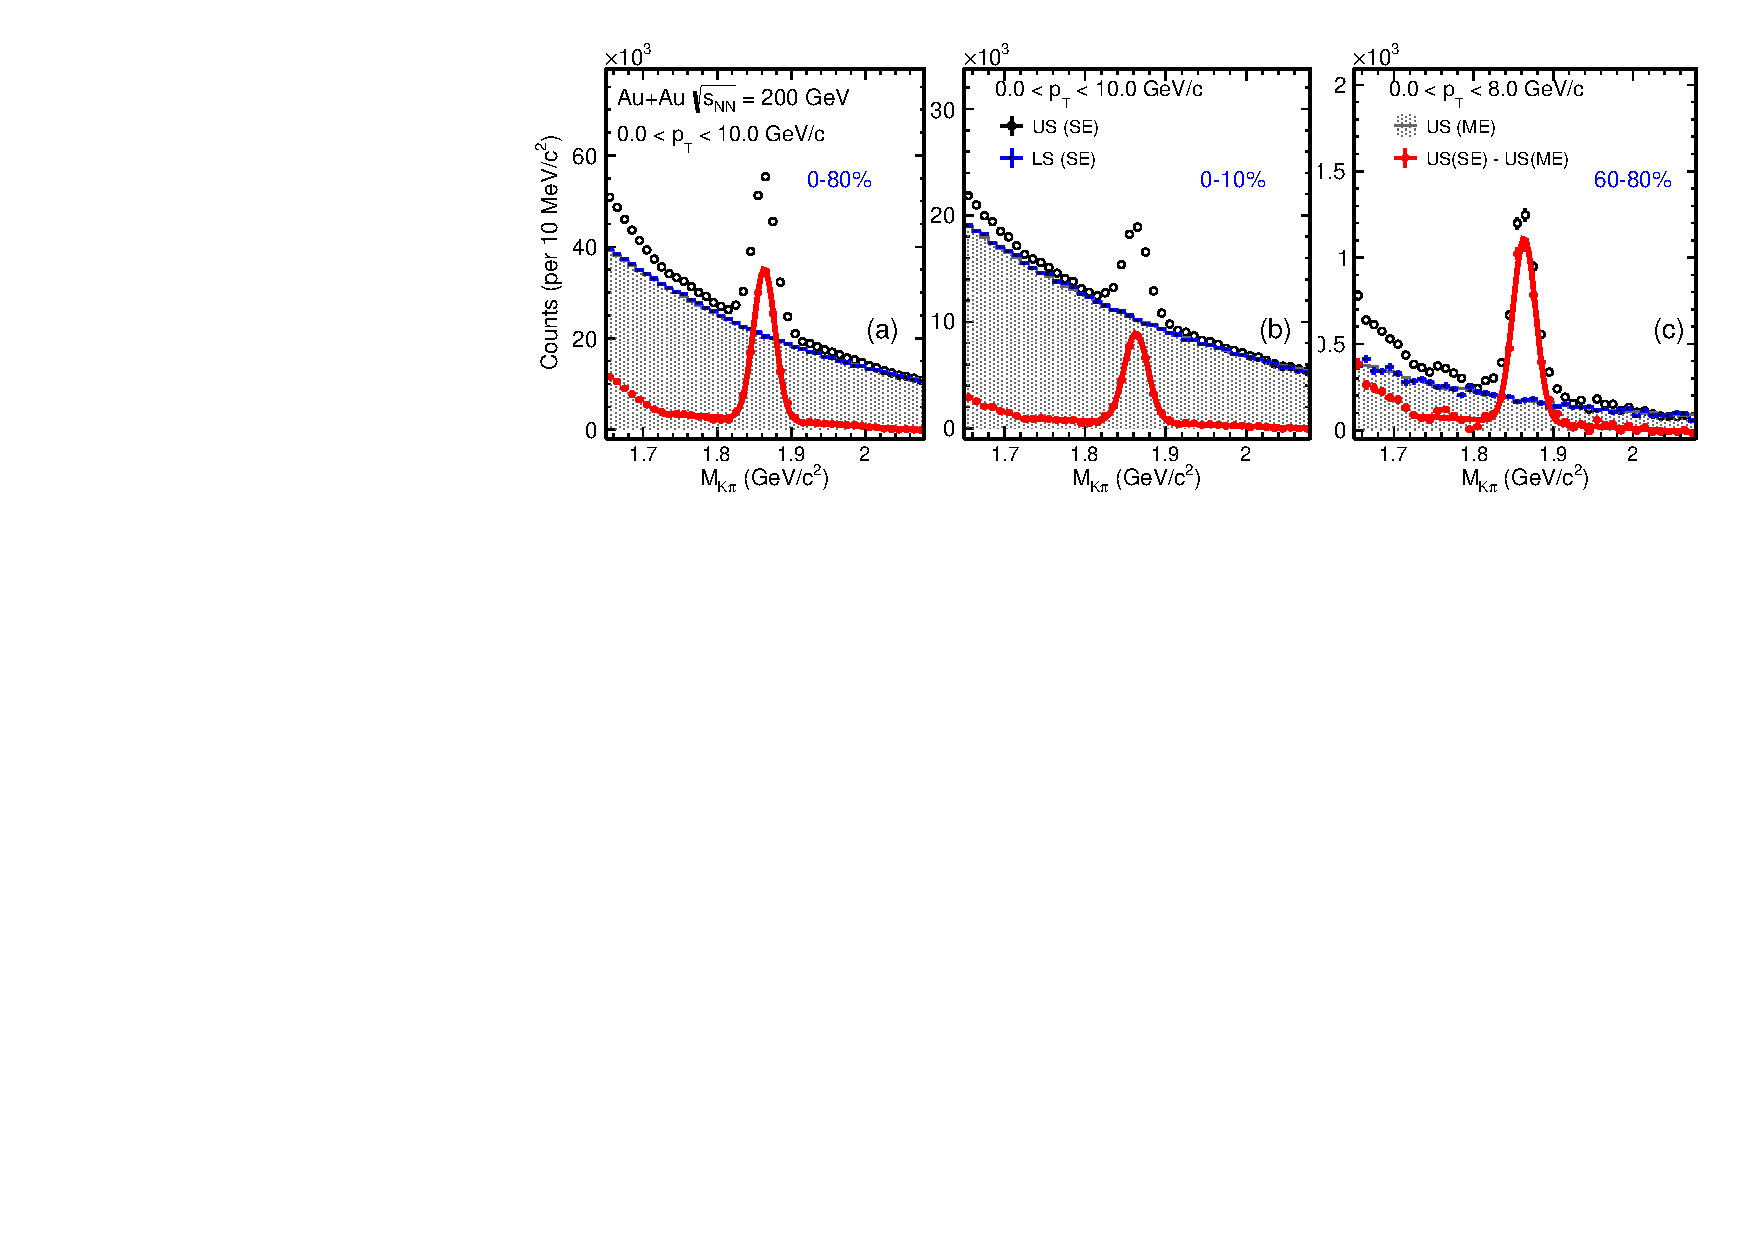
\includegraphics[width=1.0\textwidth]{fig/signal_0_8_10GeV.pdf}
\caption{Invariant mass $\rm M_{K\pi}$ distributions in \DIFdelbeginFL \DIFdelFL{$0 < p_{\rm T} < 10$ }\DIFdelendFL \DIFaddbeginFL \DIFaddFL{$0 < p_{T} < 10$ }\DIFaddendFL GeV/c from centrality bins 0--80\% (a), 0--10\% (b) and \DIFdelbeginFL \DIFdelFL{$0 < p_{\rm T} < 8$ }\DIFdelendFL \DIFaddbeginFL \DIFaddFL{$0 < p_{T} < 8$ }\DIFaddendFL GeV/c for 60--80\% (c), respectively\DIFdelbeginFL \DIFdelFL{in Au+Au collisions at $\sqrt{s_{_{\rm NN}}}$ = 200\,GeV}\DIFdelendFL . The upper limit $p_T$ range for 60--80\% stopped at 8 GeV/c since \DIFdelbeginFL \DIFdelFL{there is }\DIFdelendFL no signal \DIFaddbeginFL \DIFaddFL{was observed }\DIFaddendFL beyond \DIFaddbeginFL \DIFaddFL{within the current studies}\DIFaddendFL . \DIFaddbeginFL \DIFaddFL{US present unlike-sign pairs while LS represent like-sign pairs. SE present same-event and ME present mixed-event. The hashed region is for ME.}\DIFaddendFL }
\label{fig:signal_0} 
\end{figure*}

\begin{figure*}
\centering
% 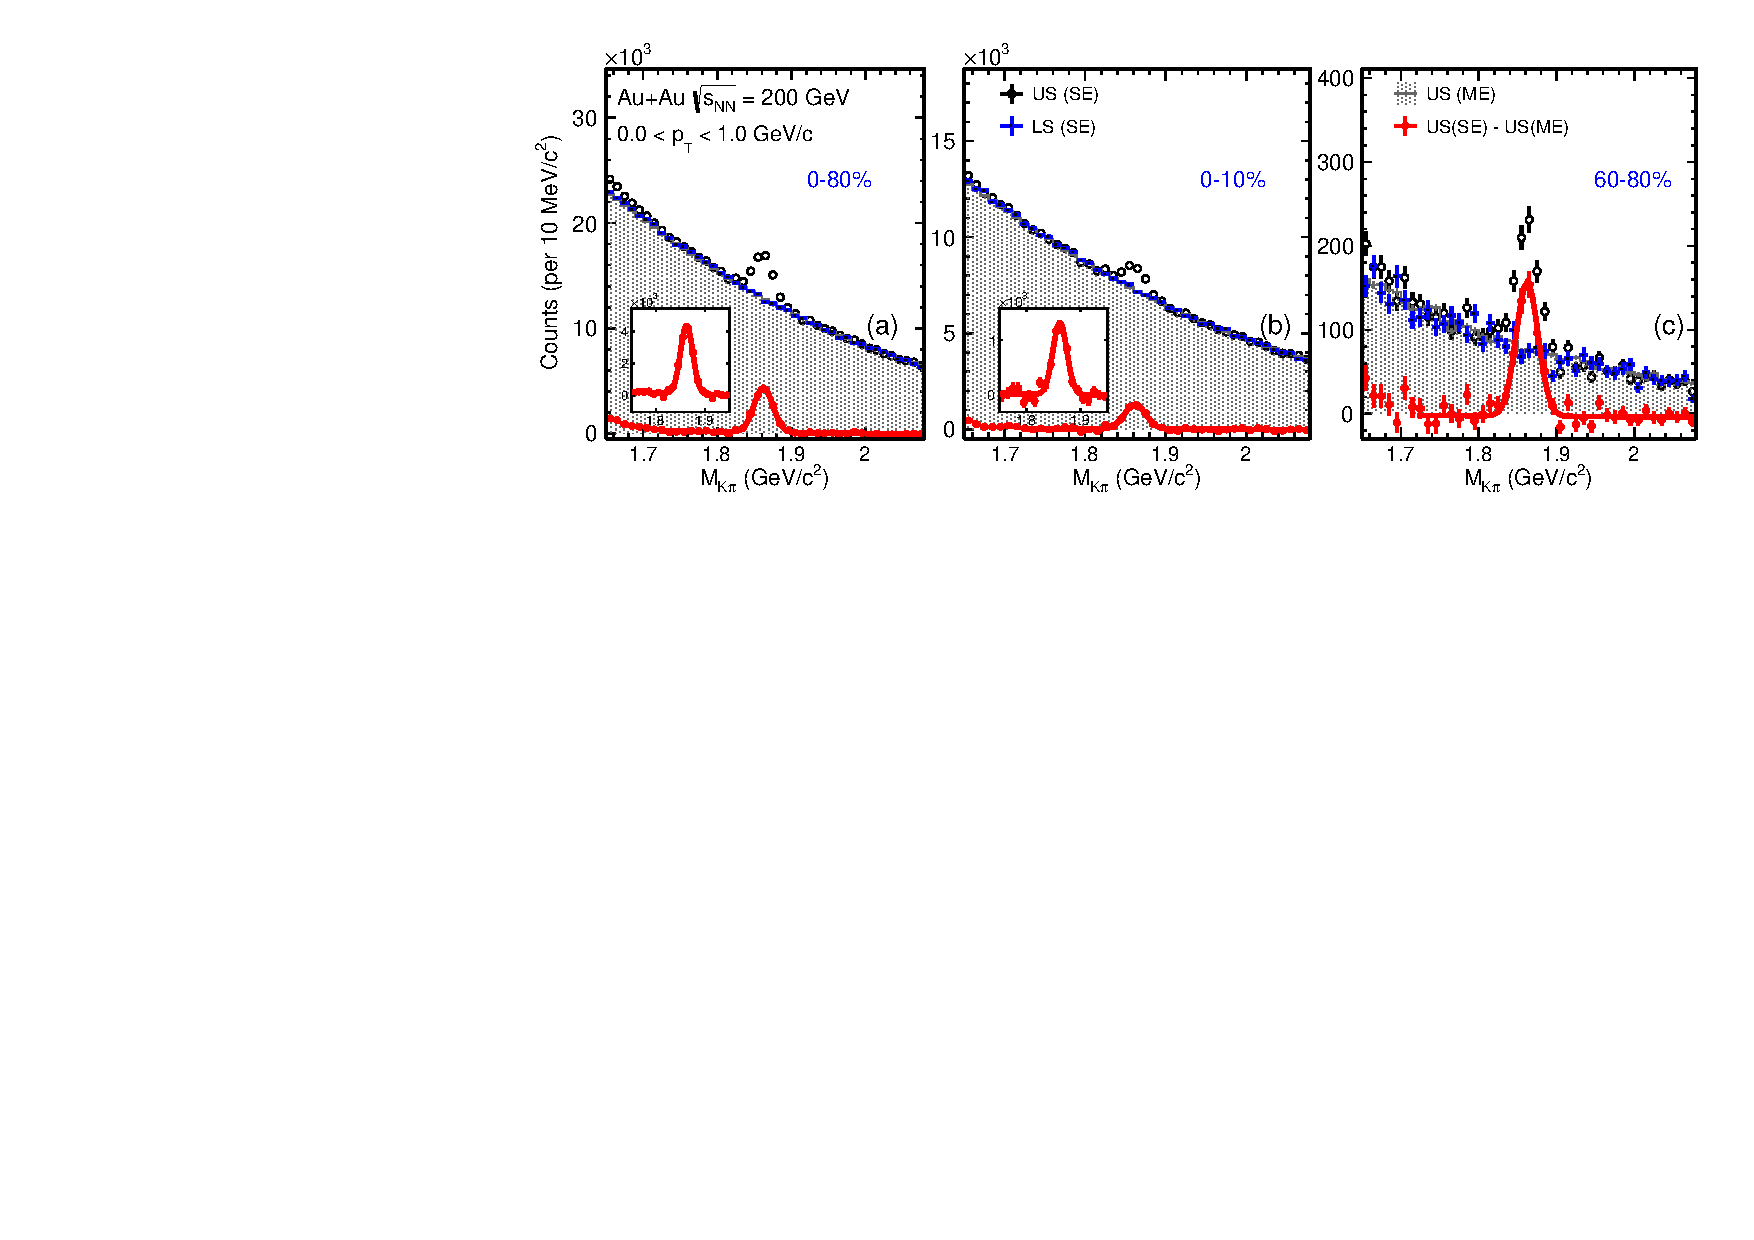
\includegraphics[width=1.0\textwidth]{fig/signal2_0_1GeV.pdf}
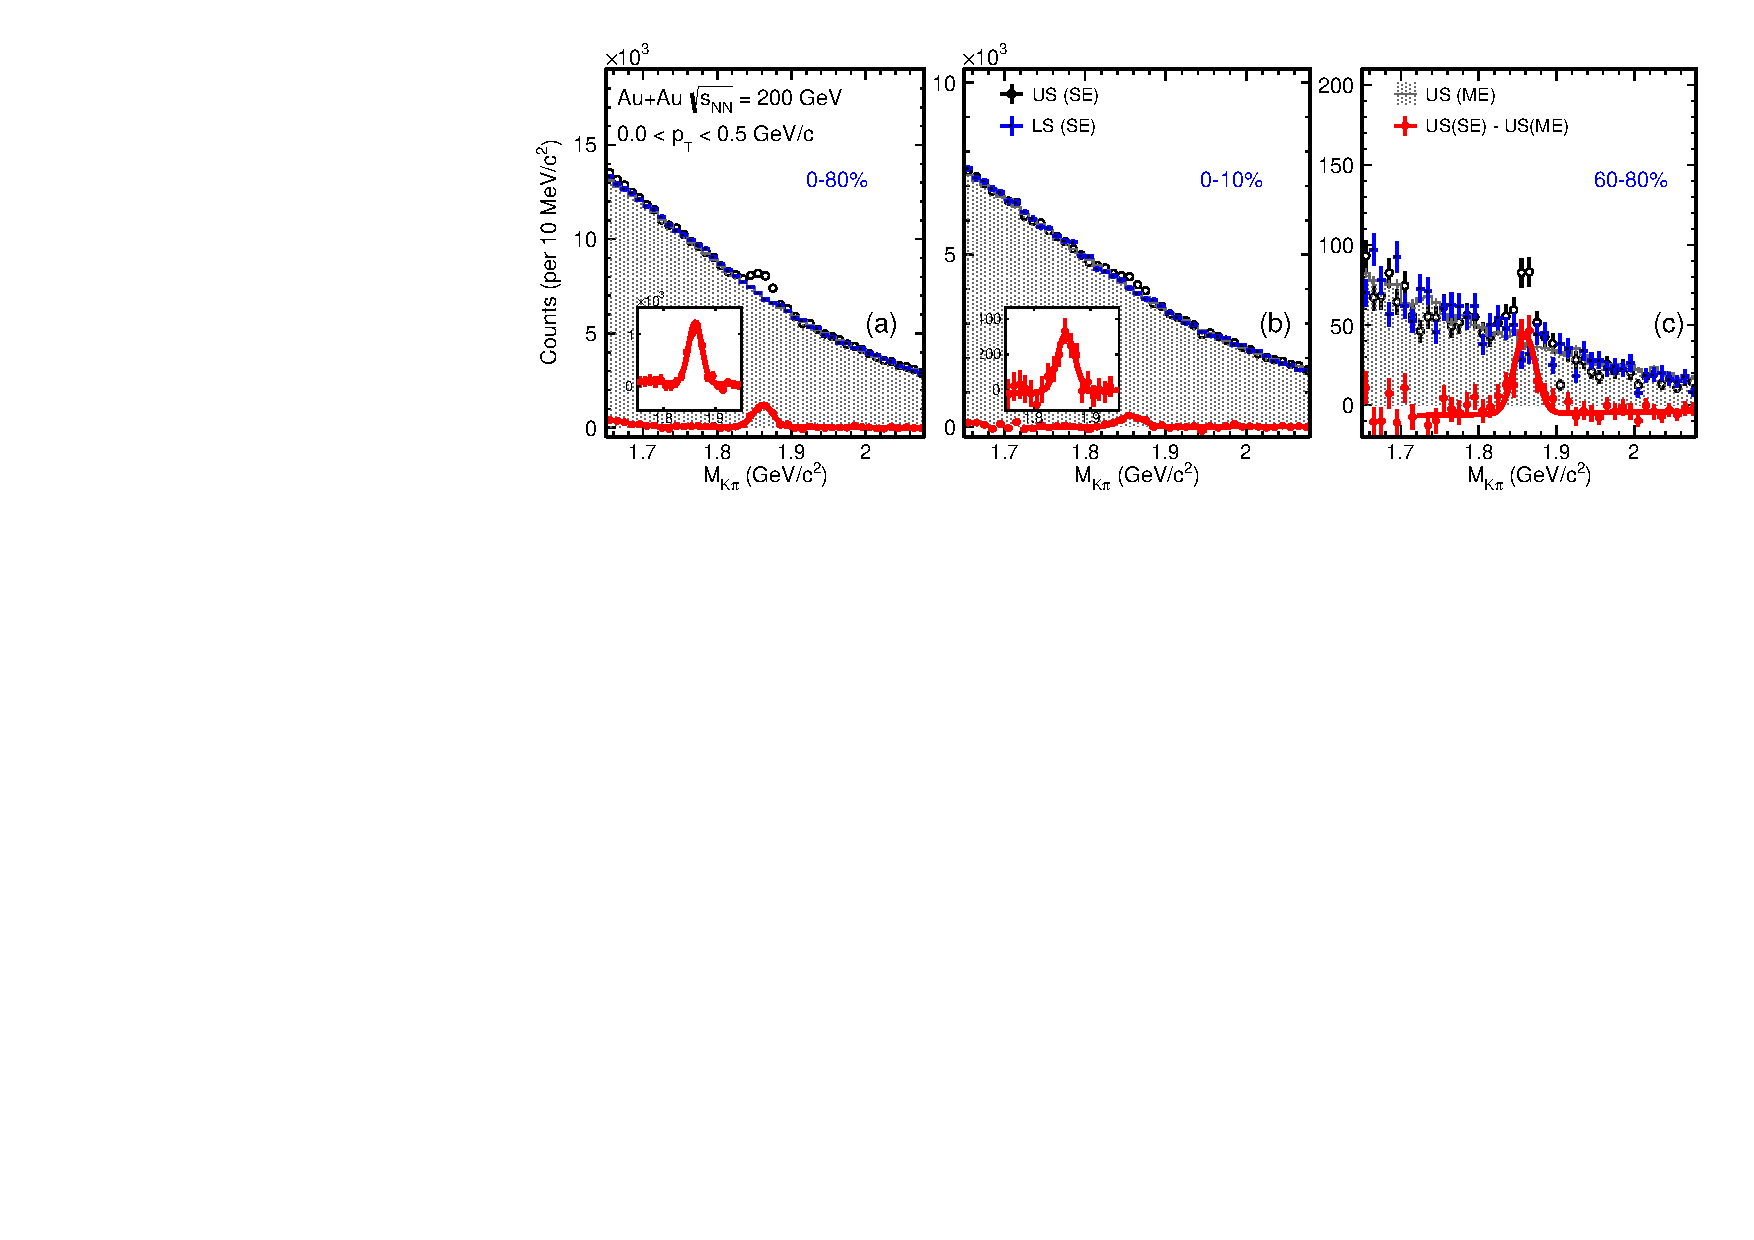
\includegraphics[width=1.0\textwidth]{fig/signal2_0_05GeV.pdf}
\caption{Invariant mass $\rm M_{K\pi}$ distributions in \DIFdelbeginFL \DIFdelFL{$0 < p_{\rm T} < 0.5$ }\DIFdelendFL \DIFaddbeginFL \DIFaddFL{$0 < p_{T} < 0.5$ }\DIFaddendFL GeV/c from centrality bins 0--80\% (a), 0--10\% (b) and 60--80\% (c), respectively\DIFdelbeginFL \DIFdelFL{in Au+Au collisions at $\sqrt{s_{_{\rm NN}}}$ = 200\,GeV}\DIFdelendFL . \DIFaddbeginFL \DIFaddFL{US, LS, SE, ME and the hashed region represent the same meanings as previous plot.}\DIFaddendFL }
\label{fig:signal_1} 
\end{figure*}

\begin{figure*}
\centering
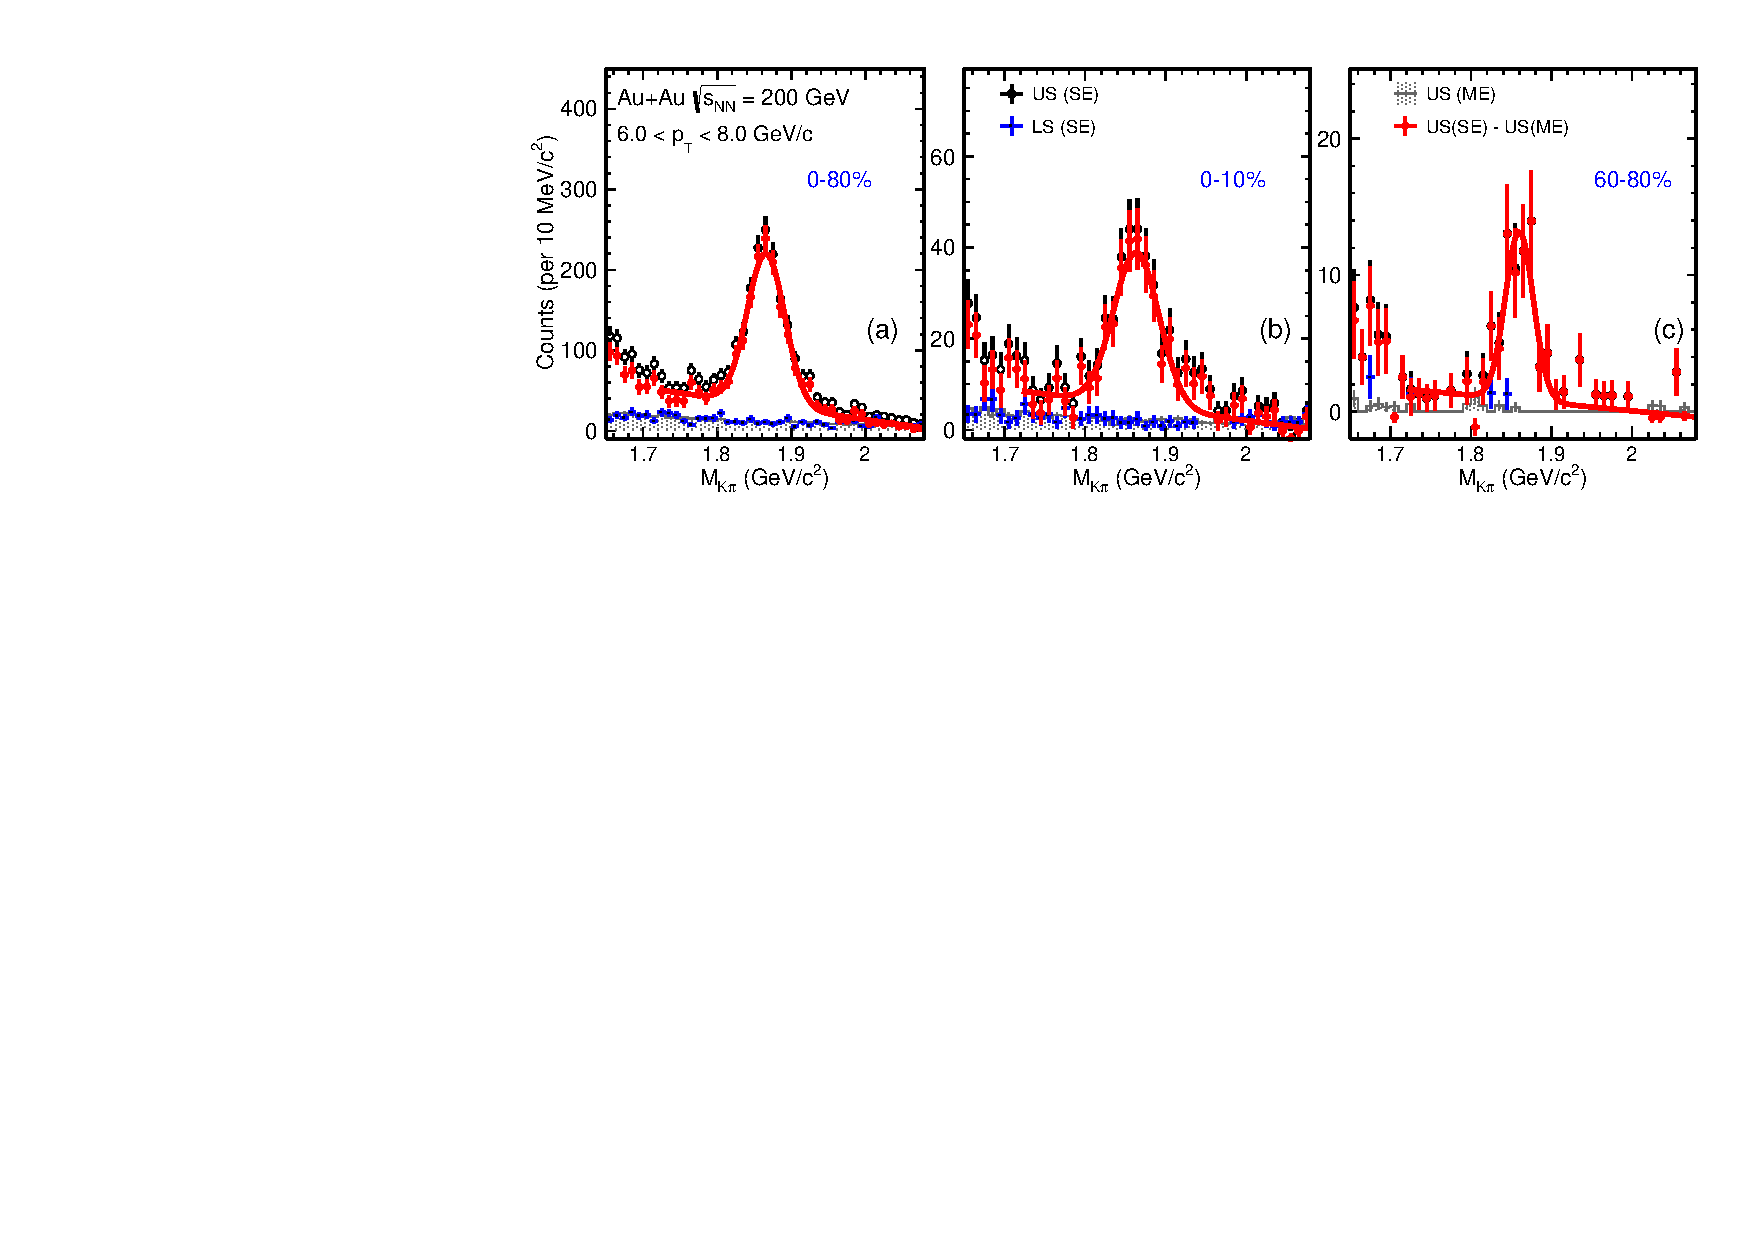
\includegraphics[width=1.0\textwidth]{fig/signal_6_8GeV.pdf}
\caption{Invariant mass $\rm M_{K\pi}$ distributions in \DIFdelbeginFL \DIFdelFL{$6 < p_{\rm T} < 8$ }\DIFdelendFL \DIFaddbeginFL \DIFaddFL{$6 < p_{T} < 8$ }\DIFaddendFL GeV/c from centrality bins 0--80\% (a), 0--10\% (b) and 60--80\% (c), respectively\DIFdelbeginFL \DIFdelFL{in Au+Au collisions at $\sqrt{s_{_{\rm NN}}}$ = 200\,GeV}\DIFdelendFL .  \DIFaddbeginFL \DIFaddFL{US, LS, SE, ME and the hashed region represent the same meaning as previous plot.}\DIFaddendFL }
\label{fig:signal_2} 
\end{figure*}

Figure~\ref{fig:signal_0} shows the invariant mass spectra of $K\pi$ pairs in \DIFaddbegin \DIFadd{$p_{T}$ 0-10 GeV/$c$ and }\DIFaddend 0-8 GeV/$c$ for three different centralities, 0-80\% minimum bias events, 0-10\% most central collisions and \DIFdelbegin \DIFdel{40-80}\DIFdelend \DIFaddbegin \DIFadd{60-80}\DIFaddend \% peripheral collisions, respectively. The combinatorial background is estimated with the same event like-sign pairs (grey) and the mixed event unlike-sign (blue) technique in which $K$ and $\pi$ from different events of similar characteristics ($V_{Z}$, centrality, event plane angle) are paired. The mixed event spectra are normalized to the like-sign distributions in the \DIFdelbegin \DIFdel{mass range from }\DIFdelend 1.7 to 2.1 GeV/$c^2$ \DIFaddbegin \DIFadd{mass range }\DIFaddend . After the subtraction of the mixed event combinatorial background from the unlike sign pairs\DIFdelbegin \DIFdel{(grey circle)}\DIFdelend , the rest are shown as red circles in the plot. Compared to the previous $D^0$ study~\cite{Star_D_RAA}, the $D^0$ signal significance is largely improved \DIFaddbegin \DIFadd{(a factor of $\sim$15) }\DIFaddend due to the combinatorial background rejection using the topological cuts enabled by the installation of HFT \DIFaddbegin \DIFadd{and optimization with TMVA}\DIFaddend . 

\DIFdelbegin \DIFdel{Figure}\DIFdelend \DIFaddbegin \DIFadd{Figures}\DIFaddend ~\ref{fig:signal_1} and \DIFdelbegin \DIFdel{Fig.~\ref{fig:signal_2} shows }\DIFdelend \DIFaddbegin \DIFadd{~\ref{fig:signal_2} show }\DIFaddend the invariant mass spectra at the same centralities as Fig.~\ref{fig:signal_0} but for different $p_T$ ranges, \DIFdelbegin \DIFdel{one }\DIFdelend \DIFaddbegin \DIFadd{Fig.~\ref{fig:signal_1} }\DIFaddend is for the lowest range 0 $< p_T <$ \DIFdelbegin \DIFdel{1 }\DIFdelend \DIFaddbegin \DIFadd{0.5 }\DIFaddend GeV/c and \DIFdelbegin \DIFdel{another one }\DIFdelend \DIFaddbegin \DIFadd{Fig.~\ref{fig:signal_2} }\DIFaddend for the highest range 6 $< p_T <$ 8 GeV/c.

After the combinatorial background is subtracted, the residual $K\pi$ invariant mass distributions are then fit by a Gaussian plus linear \DIFdelbegin \DIFdel{polynomial }\DIFdelend function. %The $D^0$ raw yields are calculated using the histogram counting within the $D^0$ mass peak region subtracting the residual background estimated via either a side-band method or a polynomial function fit.
The $D^0$ raw yields are extracted from the fits while the residual background are estimated via \DIFdelbegin \DIFdel{a polynomial }\DIFdelend \DIFaddbegin \DIFadd{the liner }\DIFaddend function fit.

\DIFaddbegin \begin{figure}
\centering
%DIF >  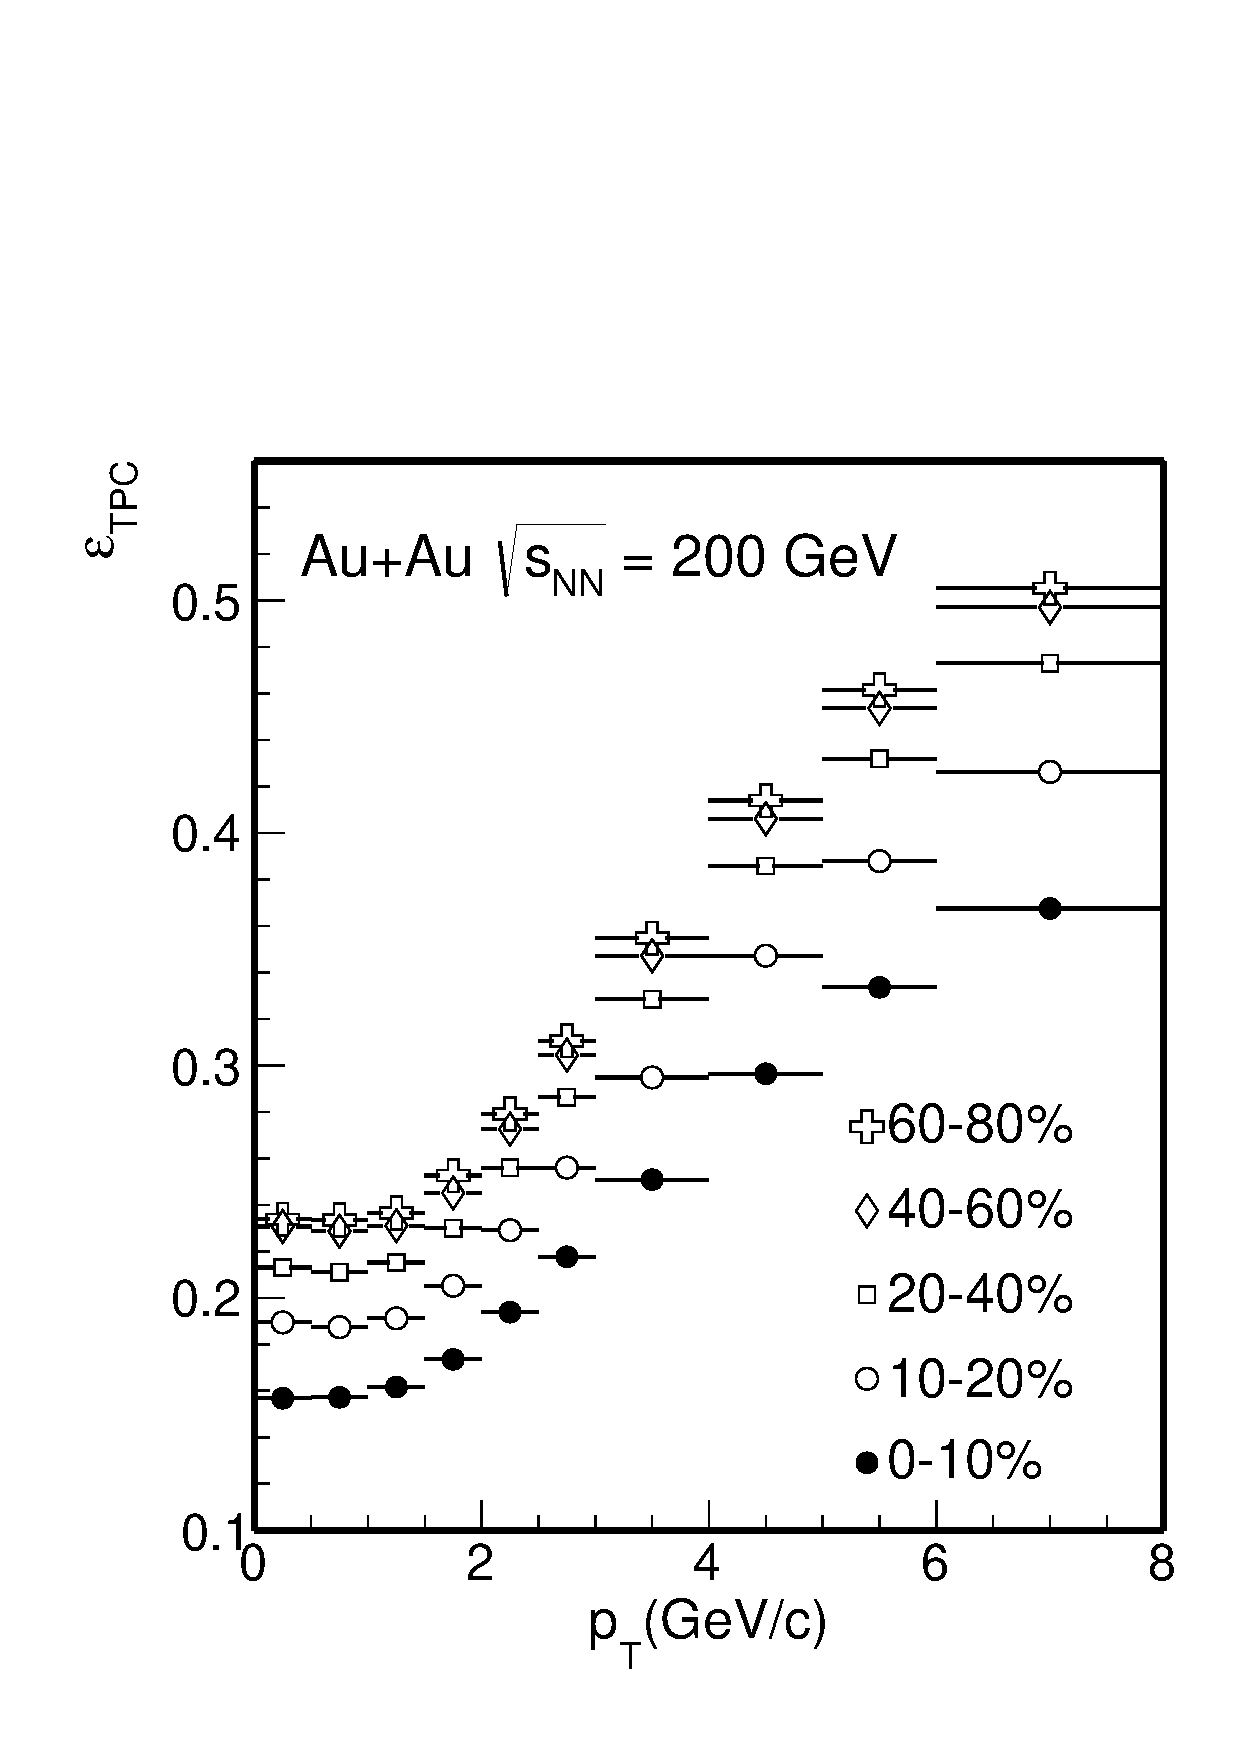
\includegraphics[width=0.4\textwidth]{fig/Datad0Eff_tpc.pdf}
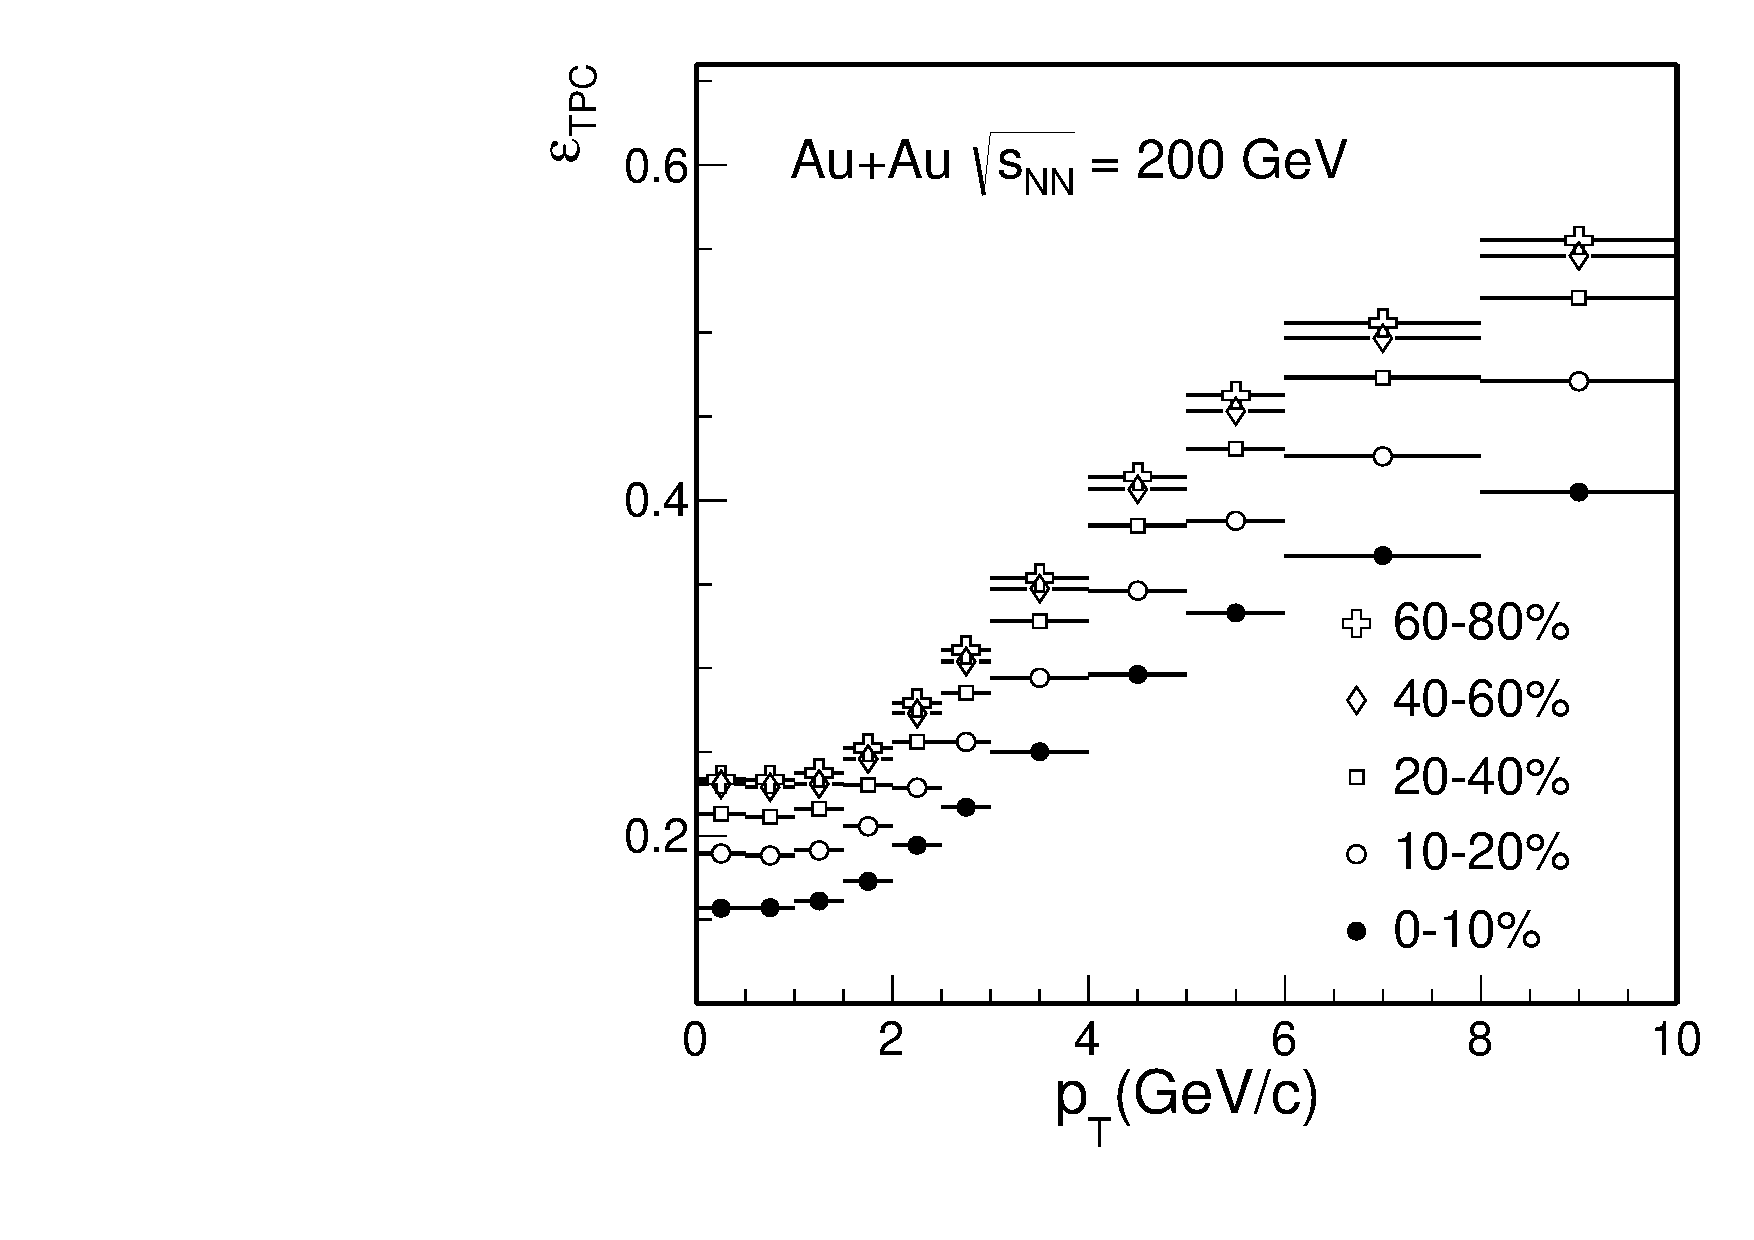
\includegraphics[width=0.43\textwidth]{fig/Datad0Eff_tpc_10.pdf}
  \caption{\DIFaddFL{$D^{0}$ TPC acceptance and tracking efficiencies from different centrality classes.}}
\label{fig:Datad0Eff_tpc} 
\end{figure}

\begin{figure*}
\centering
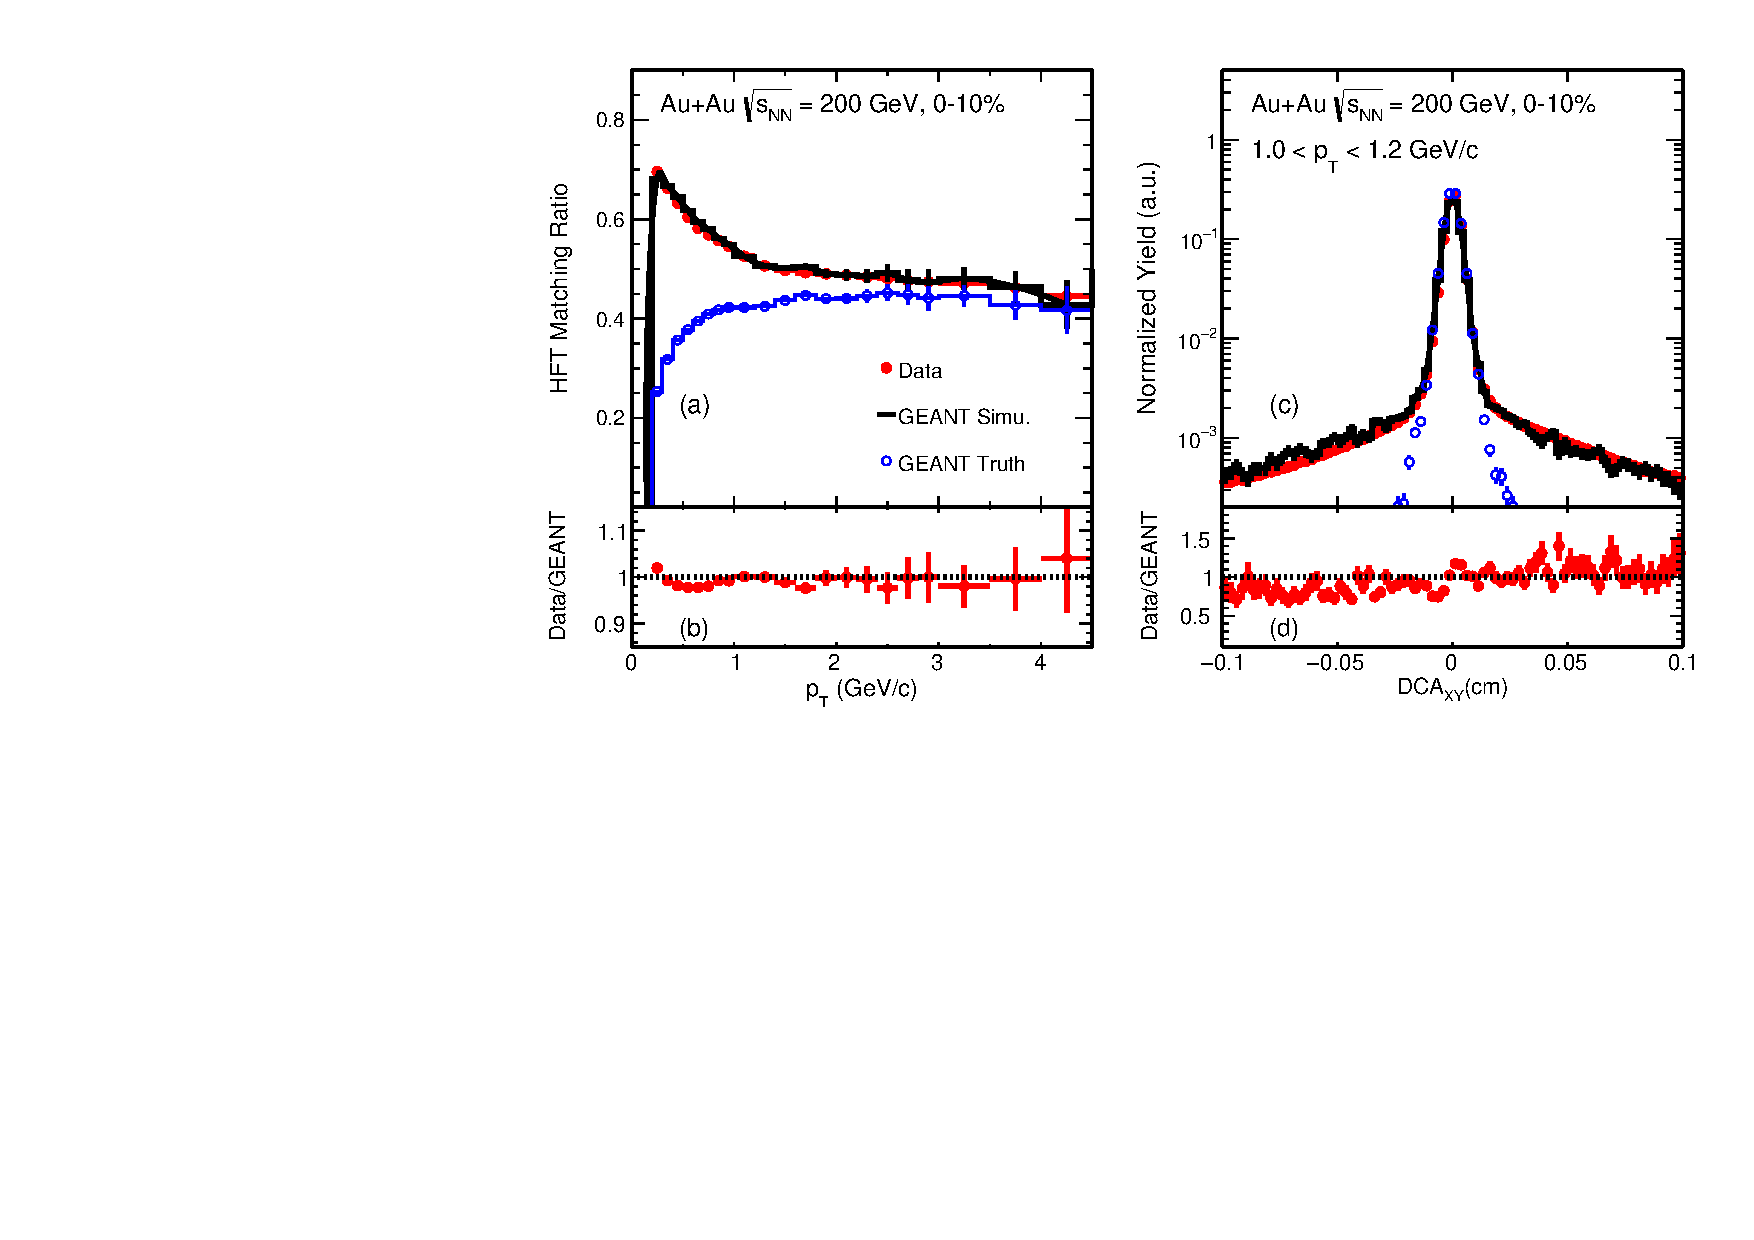
\includegraphics[width=0.85\textwidth]{fig/HijingRatioDca.pdf}
\caption{\DIFaddFL{HFT matching ratio (a) and DCA$_{\rm XY}$ (c) distributions of inclusive charged pions from real data and MC simulation in 0--10\% Au+Au collisions. The ratios between real data and GEANT simulation are shown in the bottom panels and the overall agreements are good. The blue histogram depicts the true matches with HFT hits in the GEANT simulation.}}
\label{fig:HijingRatioDca} 
\end{figure*}

\DIFaddend \section{\DIFdelbegin %DIFDELCMD < %DIFDELCMD < \label{sec:correction}%%%
%%%
\DIFdelend Efficiencies and Corrections}
\DIFaddbegin \label{correction}

\DIFaddend The reconstructed $D^0$ raw yields are calculated in each centrality, \DIFdelbegin \DIFdel{$p_{\rm T}$ bin}\DIFdelend \DIFaddbegin \DIFadd{$p_{T}$ bin, }\DIFaddend and within the rapidity window $|y|<1$. The fully corrected $D^0$ production invariant yields are calculated using the following formula\DIFdelbegin \DIFdel{.
}%DIFDELCMD < 

%DIFDELCMD < %%%
%DIF < \lipsum[1]
%DIFDELCMD < \begin{widetext}
%DIFDELCMD < %%%
\[
  \DIFdel{\frac{d^2N}{2\pi p_{\rm T}dp_{\rm T}dy} = \frac{1}{\rm B.R.} \frac{N^{\rm raw}}{N_{\rm evt} 2\pi p_{\rm T}\Delta p_{\rm T}\Delta y} \frac{1}{\varepsilon_{\rm trg}\times\varepsilon_{\rm TPC}\times\varepsilon_{\rm HFT}\times\varepsilon_{\rm PID}\times\varepsilon_{\rm vtx}}
}\]
%DIFAUXCMD
\DIFdelend \DIFaddbegin \DIFadd{:
%DIF >  \begin{widetext}
}\begin{equation}
  \DIFadd{\begin{aligned}
%\lipsum[1]
% \[
  % \frac{d^2N}{2\pi p_{T}dp_{T}dy} = \frac{1}{\rm B.R.} \frac{N^{\rm raw}}{N_{\rm evt} 2\pi p_{T}\Delta p_{T}\Delta y} \frac{1}{\varepsilon_{\rm trg}\times\varepsilon_{\rm TPC}\times\varepsilon_{\rm HFT}\times\varepsilon_{\rm PID}\times\varepsilon_{\rm vtx}}
& \frac{d^2N}{2\pi p_{T}dp_{T}dy} = \frac{1}{\rm B.R.} \times \frac{N^{\rm raw}}{N_{\rm evt} 2\pi p_{T}\Delta p_{T}\Delta y} \\
& \times \frac{1}{\varepsilon_{\rm trg}\times\varepsilon_{\rm TPC}\times\varepsilon_{\rm HFT}\times\varepsilon_{\rm PID}\times\varepsilon_{\rm vtx}},
% \end{aligned}
  }\end{equation}
\DIFaddend \label{equ:invariantyield}
\DIFdelbegin %DIFDELCMD < \end{widetext}
%DIFDELCMD < %%%
\DIFdelend %\lipsum[1]
\DIFdelbegin %DIFDELCMD < 

%DIFDELCMD < %%%
\DIFdelend \DIFaddbegin \]
%DIF >  \end{widetext}
\DIFaddend where B.R. is the $D^0\rightarrow K^-\pi^+$ decay branching ratio, (3.89$\pm$0.04)\%\DIFdelbegin \DIFdel{. }\DIFdelend \DIFaddbegin \DIFadd{~\mbox{%DIFAUXCMD
\cite{pdg}}%DIFAUXCMD
, }\DIFaddend $N^{\rm raw}$ is the reconstructed $D^0$ raw counts\DIFdelbegin \DIFdel{. }\DIFdelend \DIFaddbegin \DIFadd{, }\DIFaddend $N_{\rm evt}$ is the total numbers of events used for this analysis\DIFdelbegin \DIFdel{. }\DIFdelend \DIFaddbegin \DIFadd{, }\DIFaddend $\varepsilon_{\rm trg}$ is the centrality bias correction factor described in Sec.~\DIFdelbegin \DIFdel{\ref{sec:dataset:trigger}}\DIFdelend \DIFaddbegin \DIFadd{\ref{dataset:trigger}}\DIFaddend . The raw yields need to be corrected for the TPC acceptance and tracking efficiency - $\varepsilon_{\rm TPC}$, the HFT acceptance and tracking plus topological cut efficiency - $\varepsilon_{\rm HFT}$, the particle identification efficiency - $\varepsilon_{\rm PID}$\DIFaddbegin \DIFadd{, }\DIFaddend and the finite vertex resolution correction - $\varepsilon_{\rm vtx}$\DIFdelbegin \DIFdel{, mostly in small multiplicity peripheral events.
These four corrections will be discussed in detail in the following part of this sub-section}\DIFdelend .

\subsection{\DIFdelbegin %DIFDELCMD < %DIFDELCMD < \label{sec:correction:tpc}%%%
%%%
\DIFdelend TPC Acceptance and Tracking Efficiency - $\varepsilon_{\rm TPC}$}
\DIFaddbegin \label{correction:tpc}
\DIFaddend 

The TPC acceptance and tracking efficiency is obtained using the standard STAR TPC embedding technique, in which a small amount of MC tracks (typically 5\% of the total multiplicity of the real event) are processed through the full GEANT simulation\DIFaddbegin \DIFadd{~\mbox{%DIFAUXCMD
\cite{GEANT4}}%DIFAUXCMD
}\DIFaddend , then mixed with the raw Data Acquisition (DAQ) data in real events and reconstructed through the same reconstruction chain as the real data production. The TPC efficiency is then calculated as the ratio of the reconstructed MC tracks with the same offline analysis cuts for geometric acceptance and other TPC requirements to the input MC tracks.

Figure~\ref{fig:Datad0Eff_tpc} shows the TPC acceptance and tracking \DIFdelbegin \DIFdel{efficiencies }\DIFdelend \DIFaddbegin \DIFadd{efficiency }\DIFaddend $\varepsilon_{\rm TPC}$ for $D^0$ mesons in various centrality classes in \DIFdelbegin \DIFdel{Au+Au collisions at $\sqrt{s_{_{\rm NN}}}$ = 200\,GeV in }\DIFdelend this analysis. The efficiencies include the TPC and analysis acceptance cuts \DIFdelbegin \DIFdel{$p_{\rm T}>0.6$}\DIFdelend \DIFaddbegin \DIFadd{$p_{T}>0.6$}\DIFaddend \,GeV/$c$ and $|\eta|<1$ as well as the TPC tracking efficiency for both pion and kaon daughters. The lower efficiency observed in central collisions is due to the increased multiplicity, and therefore higher occupancy, in these collisions.


\begin{figure}
\centering
%DIF <  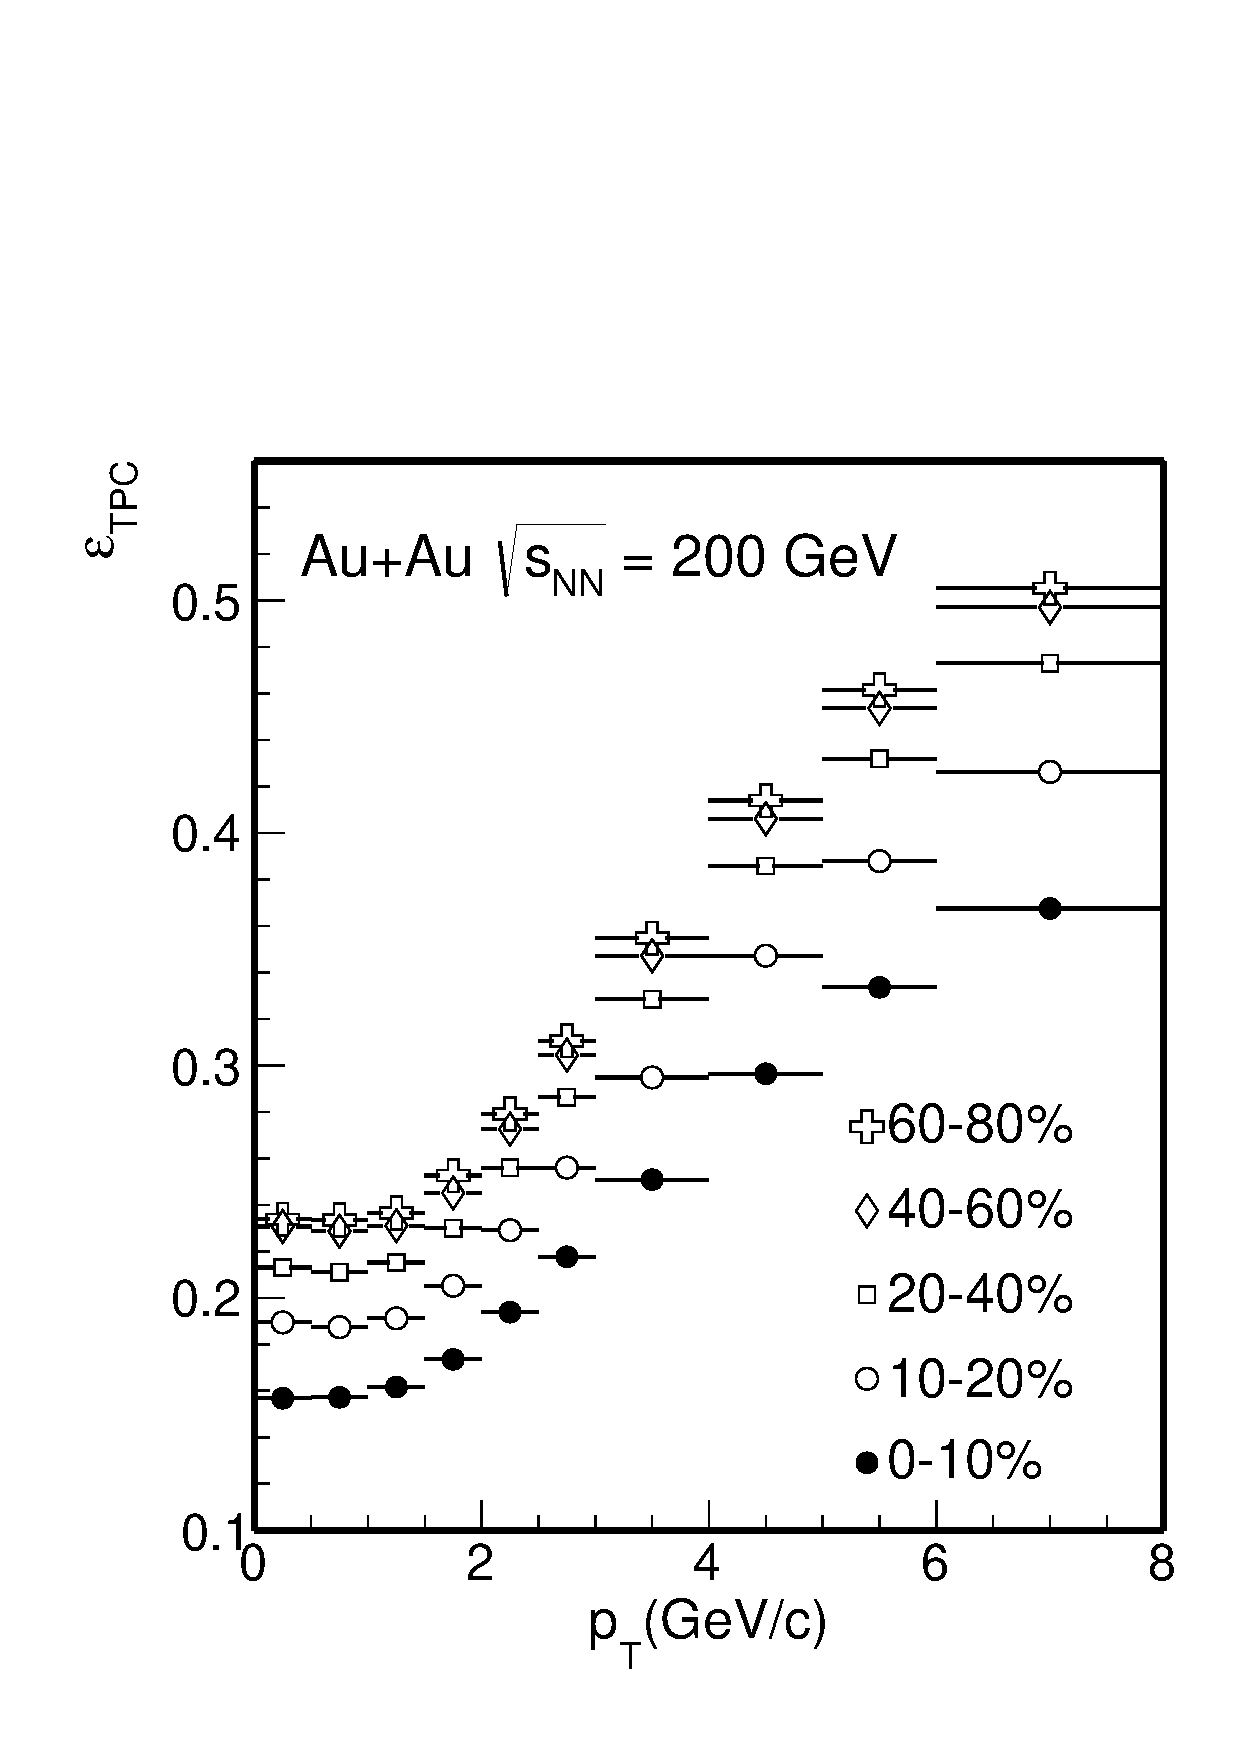
\includegraphics[width=0.4\textwidth]{fig/Datad0Eff_tpc.pdf}
\DIFdelbeginFL %DIFDELCMD < 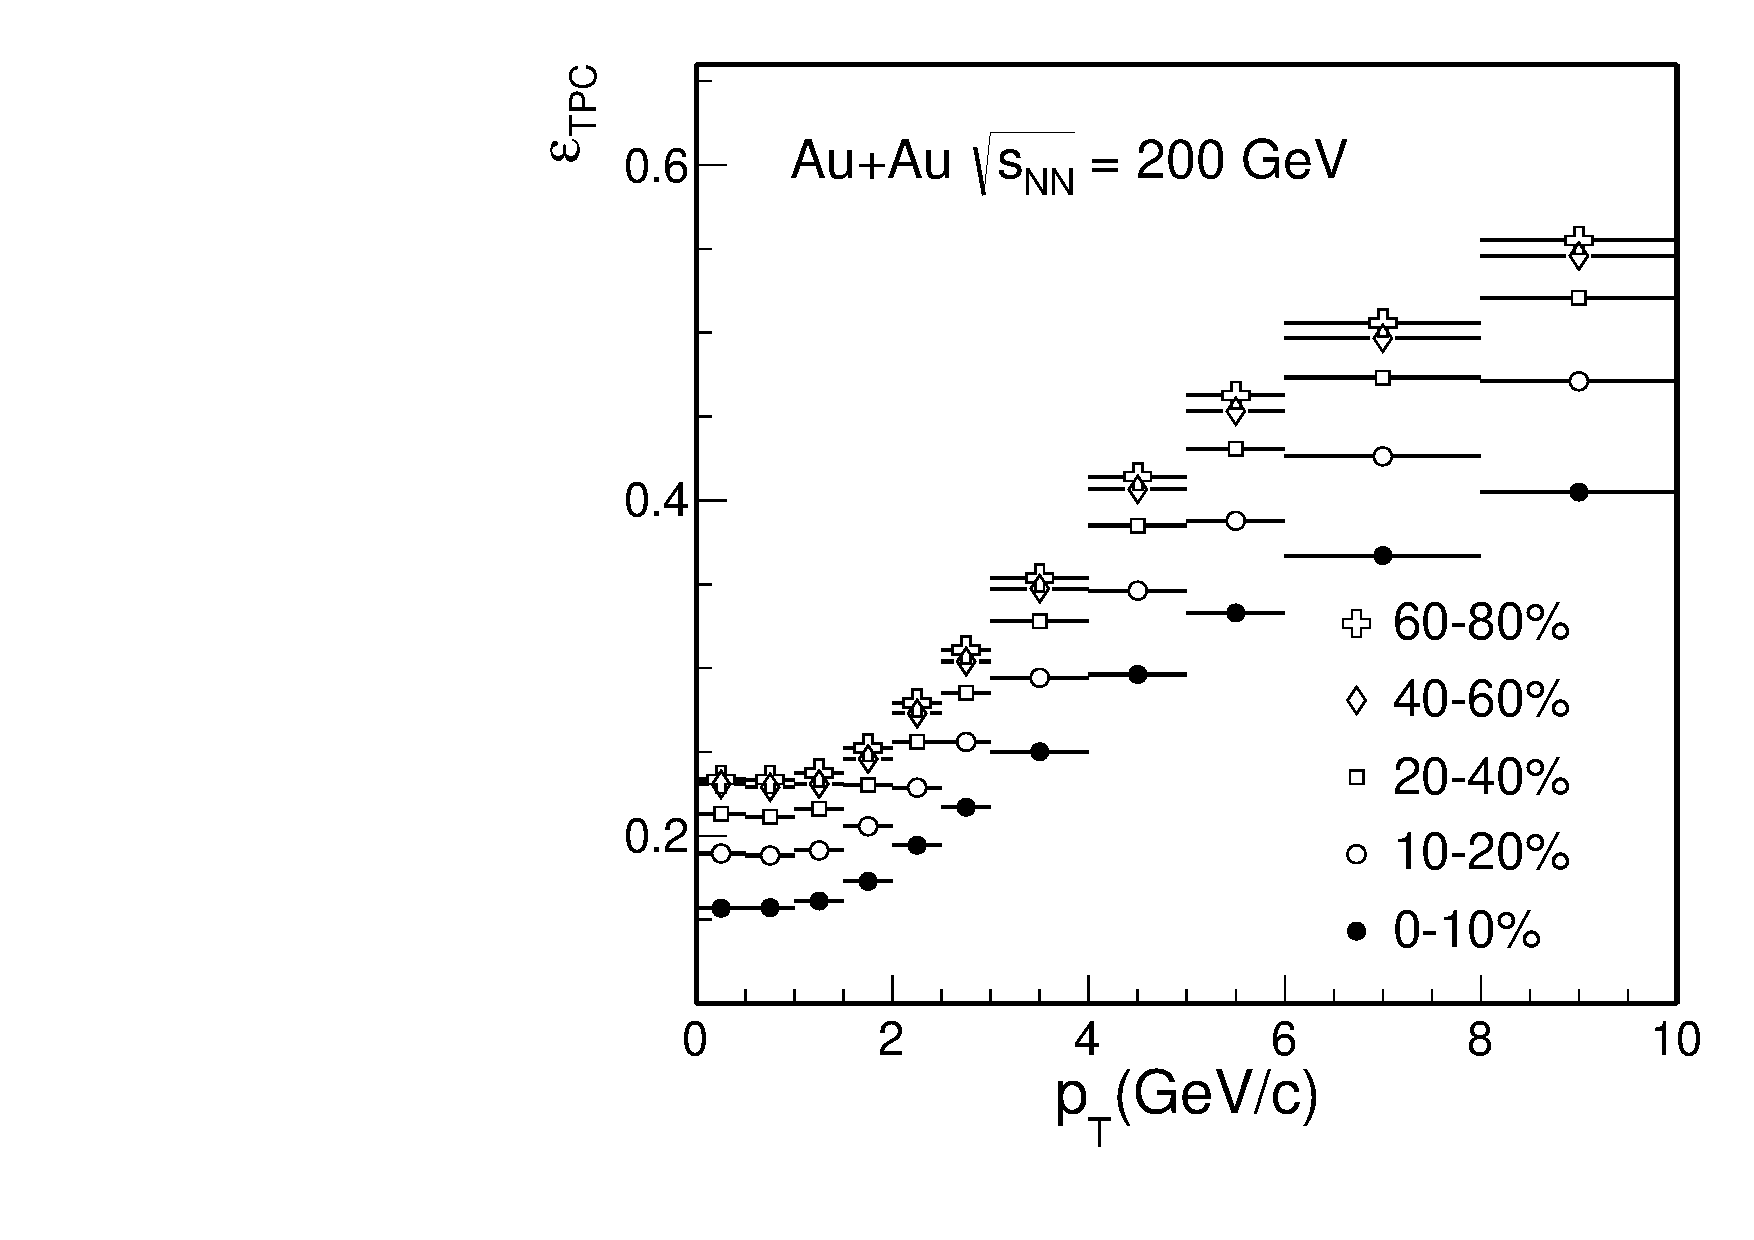
\includegraphics[width=0.43\textwidth]{fig/Datad0Eff_tpc_10.pdf}
%DIFDELCMD < %%%
\DIFdelendFL \DIFaddbeginFL 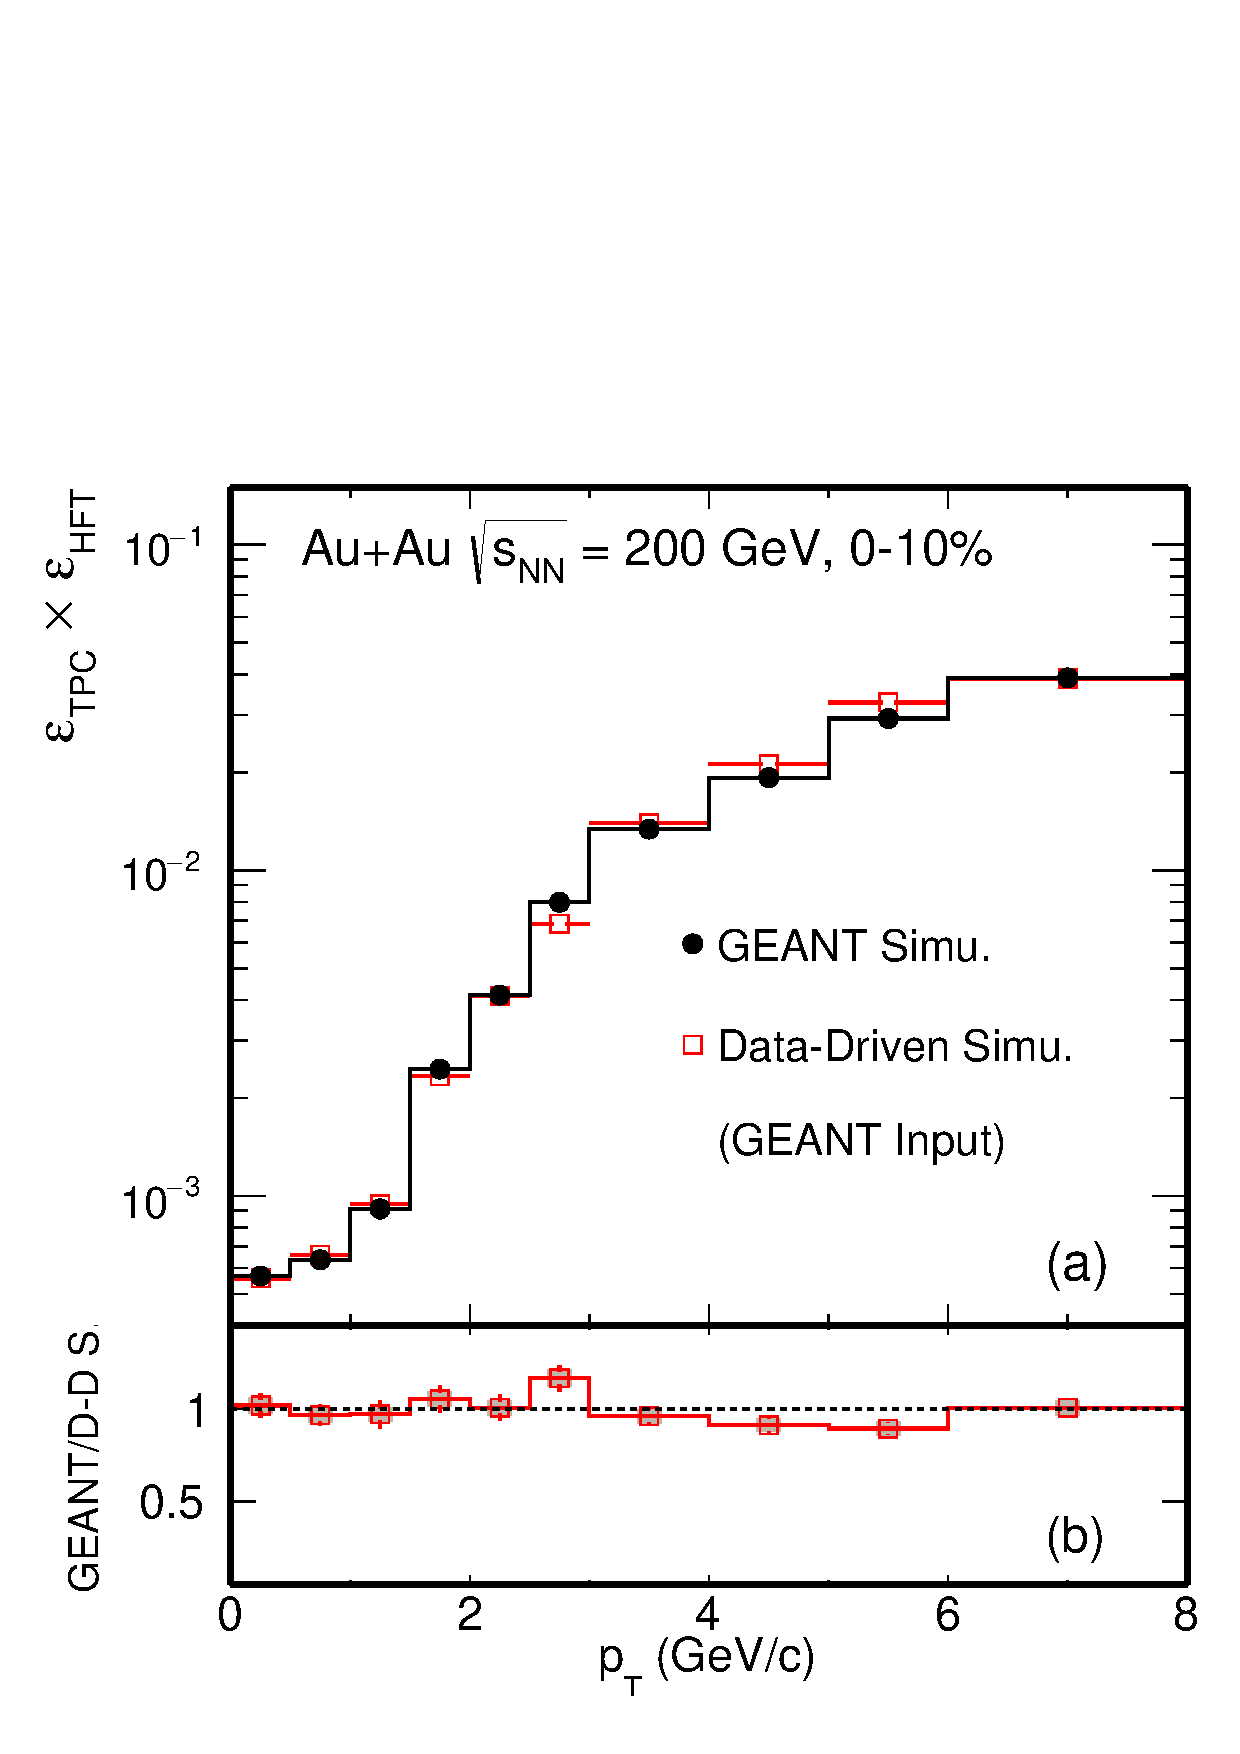
\includegraphics[width=0.43\textwidth]{fig/Mcd0Eff_0_10.pdf}
\DIFaddendFL \caption{$D^{0}$ \DIFdelbeginFL \DIFdelFL{TPC acceptance }\DIFdelendFL \DIFaddbeginFL \DIFaddFL{reconstruction efficiency comparison between MC simulation $(black)$ }\DIFaddendFL and \DIFdelbeginFL \DIFdelFL{tracking efficiencies from different centrality classes }\DIFdelendFL \DIFaddbeginFL \DIFaddFL{data-driven fast simulation with the reconstructed distributions }\DIFaddendFL in \DIFaddbeginFL \DIFaddFL{the simulation sample as an input $(red)$ in central 0-10\% }\DIFaddendFL Au+Au collisions\DIFdelbeginFL \DIFdelFL{at $\sqrt{s_{_{\rm NN}}}$ = 200\,GeV}\DIFdelendFL .}
\DIFdelbeginFL %DIFDELCMD < \label{fig:Datad0Eff_tpc} 
%DIFDELCMD < %%%
\DIFdelendFL \DIFaddbeginFL \label{fig:Mcd0Eff_0_10} 
\DIFaddendFL \end{figure}


\DIFdelbegin \subsection{%DIFDELCMD < %DIFDELCMD < \label{sec:correction:hft}%%%
%%%
\DIFdel{HFT Acceptance, Tracking and Topological Cut Efficiency - $\varepsilon_{\rm HFT}$}}
%DIFAUXCMD
\addtocounter{subsection}{-1}%DIFAUXCMD
\DIFdelend \DIFaddbegin \begin{figure*}
\centering
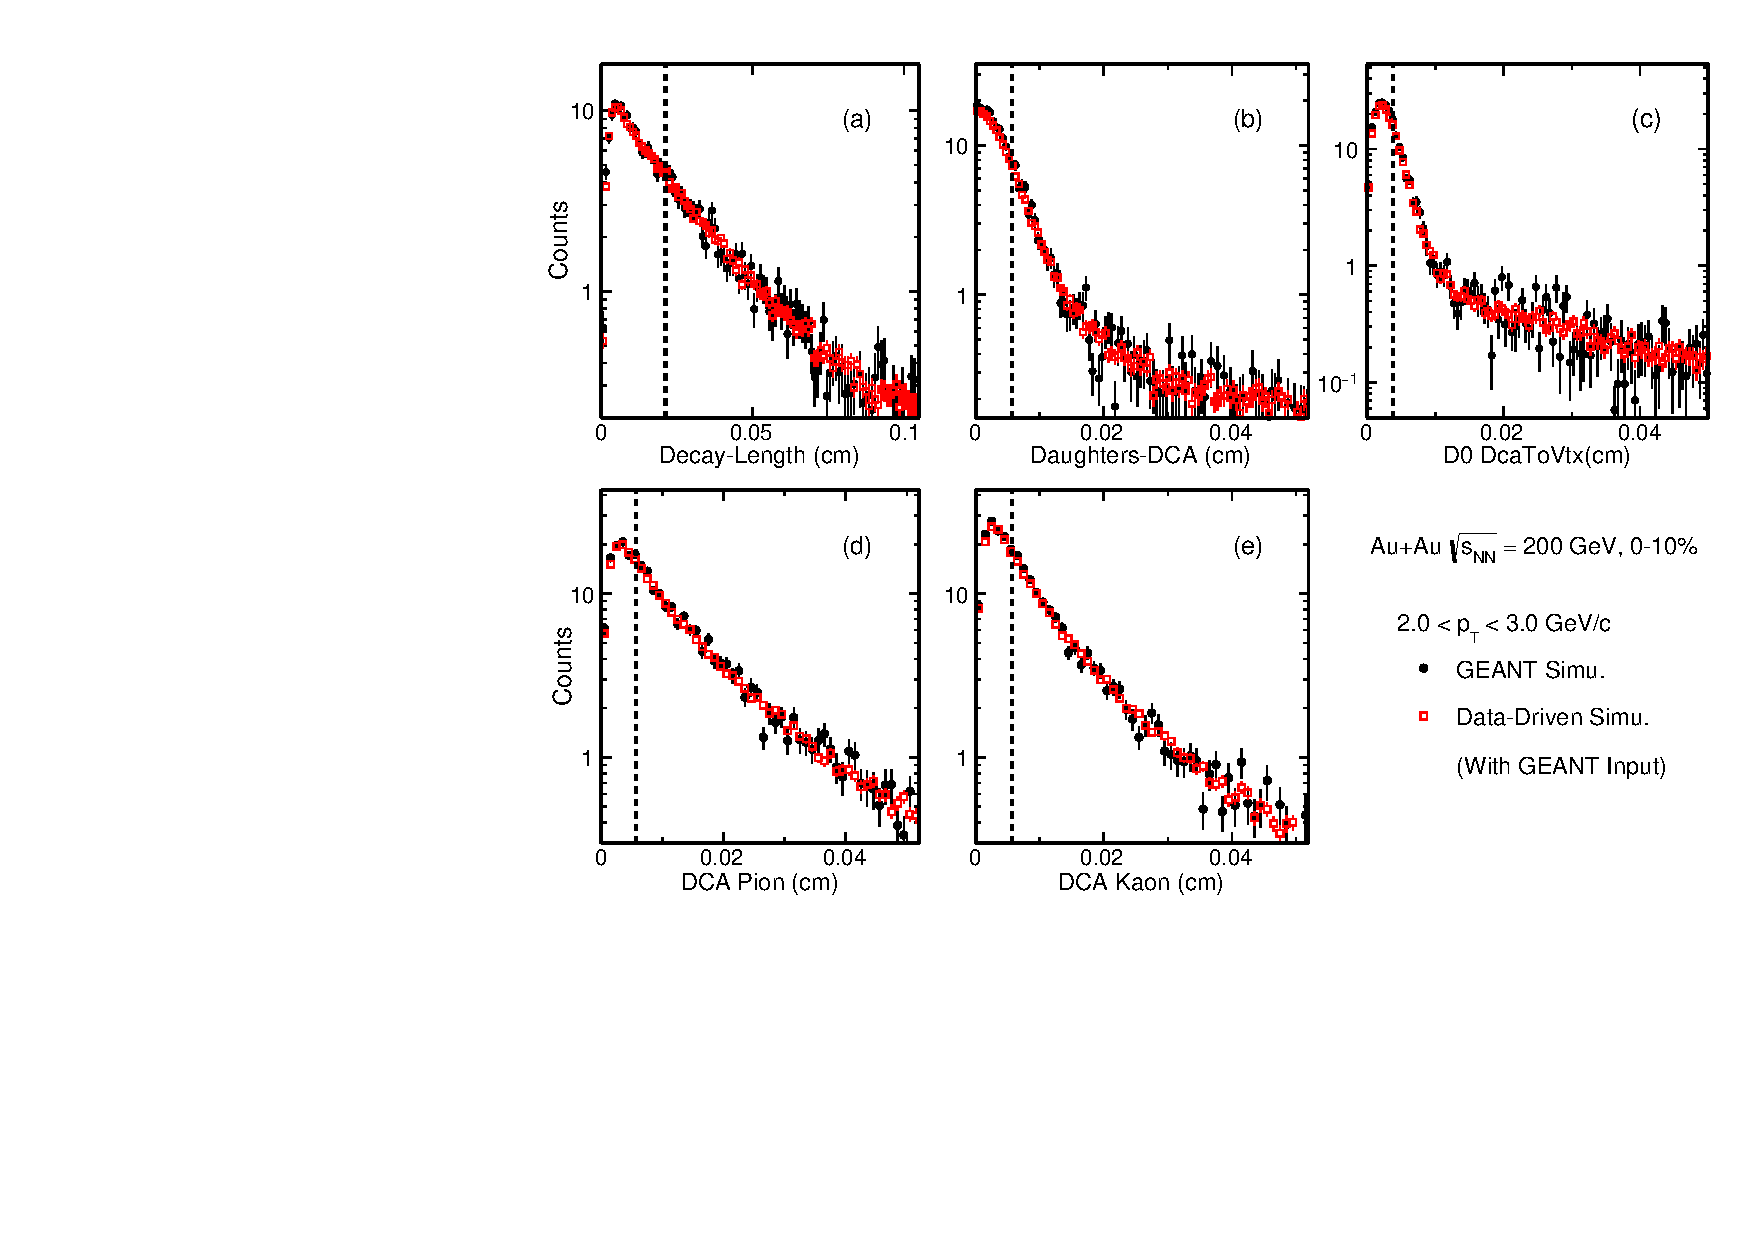
\includegraphics[width=1.0\textwidth]{fig/McTopo.pdf}
\caption{\DIFaddFL{Topological distributions comparison between MC GEANT simulation $(black)$ and data-driven fast simulation with the reconstructed distributions in the simulation sample as an input $(red)$ in most central (0--10\%) Au+Au collisions.}}
\label{fig:McTopo} 
\end{figure*}
\DIFaddend 


\DIFdelbegin \subsubsection{%DIFDELCMD < %DIFDELCMD < \label{sec:correction:hft:fastsim}%%%
%%%
\DIFdel{Data-driven Simulation}}
%DIFAUXCMD
\addtocounter{subsubsection}{-1}%DIFAUXCMD
\DIFdelend \DIFaddbegin \subsection{\DIFadd{HFT Acceptance, Tracking and Topological Cut Efficiency - $\varepsilon_{\rm HFT}$}}
\label{correction:hft}
\DIFaddend 

\DIFaddbegin \subsubsection{\DIFadd{Data-driven Simulation}} 
\label{correction:hft:fastsim}

\DIFaddend Since the performance of the HFT changes with time, in order to fully capture the real-time detector performance\DIFaddbegin \DIFadd{, }\DIFaddend the HFT-related efficiency is obtained using a data-driven simulation method in this analysis. The performance of inclusive HFT tracks is characterized by a TPC-to-HFT matching ratio and the DCA distributions. These distributions obtained from real data are fed into a Monte Carlo decay generator for $D^0\rightarrow K^-\pi^+$ and followed by the same reconstruction of $D^0$ secondary vertex as in real data. The same topological cuts are then \DIFdelbegin \DIFdel{be }\DIFdelend applied and the HFT related efficiency for the $D^0$ reconstruction is \DIFdelbegin \DIFdel{then }\DIFdelend calculated.

% To obtain the real invariant mass spectrum of $D^0$ within STAR acceptance ($|\eta_{\pi}| \leq 1, |\eta_{K}| \leq 1, |Y_{K\pi}| \leq 1$), the $D^0$ raw spectrum should correct for the efficiency. The $K\pi$ pair efficiency within STAR acceptance is evaluated by folding the TPC related efficiency to the HFT related efficiency as shown on Eq.~\ref{effEqu1} and Eq.~\ref{effEqu2}. For the TPC related tracking efficiency shows on the first term, we use STAR standard Full GEANT simulation. For the HFT related efficiency include the second and third terms which reflect to HFT acceptance and topological cuts, the developed `Data-Driven Fast simulation' which will discuss following.

% \begin{equation}
%   % \textup{Eff.} \times \textup{Accept.}  = \textup{TPC Tracking Eff.} \otimes \textup{HFT Tracking Eff.} \otimes \textup{Topollogy Cuts}
%   \textup{Eff.} \times \textup{Accept.}  = \textup{TPC Tracking Eff.} \otimes \textup{HFT Related Eff.}
% \label{effEqu1}
% \end{equation}

% \begin{equation}
%   \textup{HFT Related Eff.}  =\textup{HFT Tracking Eff.} \otimes \textup{Topology Cuts}
% \label{effEqu2}
% \end{equation}

To best represent the \DIFdelbegin \DIFdel{detector real }\DIFdelend \DIFaddbegin \DIFadd{real detector }\DIFaddend performance, we obtain the following distributions from real data in this Monte Carlo approach.
 \begin{itemize} 
\item Centrality-dependent $\textup{V}_\textup{z}$ distributions.
\item Ratios of HFT matched tracks to TPC tracks, including the dependence on particle species, centrality, $p_T$, $\eta$, $\phi$, and $\textup{V}_\textup{z}$.
\item $\textup{DCA}_{\textup{XY}}$ - $\textup{DCA}_{\textup{Z}}$ \DIFdelbegin \DIFdel{2-dimension }\DIFdelend \DIFaddbegin \DIFadd{2-dimensional }\DIFaddend (2D) distributions including the dependence on particle species, centrality, $p_T$, $\eta$, and $\textup{V}_\textup{z}$.
 \end{itemize} 
The $\textup{DCA}_{\textup{XY}}$ - $\textup{DCA}_{\textup{Z}}$ 2D distributions are the key to represent not only the right matches, but also the fake matches when connecting the TPC tracks with HFT hits. The distributions are obtained in 2D to consider the correlation between the two quantities and therefore to reproduce the 3D DCA position distributions. The $\phi$ dependence of these distributions are integrated over due to computing resource limits, but we have checked the $\phi$ dependence (by reducing other \DIFdelbegin \DIFdel{dependences }\DIFdelend \DIFaddbegin \DIFadd{dependencies }\DIFaddend for the same reason) and it \DIFdelbegin \DIFdel{produces a consistent efficiency result compared }\DIFdelend \DIFaddbegin \DIFadd{gives a consistent result compare }\DIFaddend to the $\phi$\DIFdelbegin \DIFdel{-degenerated result we use here as the default}\DIFdelend \DIFaddbegin \DIFadd{-integrated one}\DIFaddend .

In total, there are 11 ($\phi$) $\times$ 10 ($\eta$) $\times$ 6 ($\textup{V}_\textup{z}$) $\times$ 9 (centrality) $\times$ 2 (particles) 1D histograms (36 $p_T$ bins each) used for the HFT match ratio distributions and 5 ($\eta$) $\times$ 4 ($\textup{V}_\textup{z}$) $\times$ 9 (centrality) $\times$ 2 (particles) $\times$ 19 ($p_T$) 2D histograms (144 \DIFaddbegin \DIFadd{$\textup{DCA}_{\textup{XY}}$ }\DIFaddend $\times$ 144 \DIFdelbegin \DIFdel{DCA binning}\DIFdelend \DIFaddbegin \DIFadd{$\textup{DCA}_{\textup{Z}}$ bins}\DIFaddend ) for 2D DCA distributions. The number of bins chosen is optimized to balance the need of computing resources as well as the stability of the final efficiency. All dimensions have been checked so that further increase in the number of bins (in balance we need to reduce the number of bins in other dimensions)  will not change the final obtained efficiency.

The procedure for this data-driven simulation package for efficiency calculation is as follows:

% After all the input ingredients ready for the fast-simulation, a simple toy MC simulation (PYTHIA) is applied for the efficiency study. The basic recipe is following:
 \begin{itemize} 
\item Sample $\textup{V}_\textup{z}$ distribution according to \DIFdelbegin \DIFdel{data distribution }\DIFdelend \DIFaddbegin \DIFadd{the distribution obtained from the real data}\DIFaddend .
\item Generate $D^0$ at the event vertex position with desired $p_T$ (\DIFdelbegin \DIFdel{levy }\DIFdelend \DIFaddbegin \DIFadd{Levy }\DIFaddend shape fitted to $D^0$ spectra) and rapidity (flat) distributions.
\item \DIFdelbegin \DIFdel{Let }\DIFdelend \DIFaddbegin \DIFadd{Propagate }\DIFaddend $D^0$ \DIFdelbegin \DIFdel{fly and }\DIFdelend \DIFaddbegin \DIFadd{and simulate it's }\DIFaddend decay to $K^-\pi^+$ daughters following the decay probability.
\item Smear daughter track momentum according to the values obtained from embedding.
\item Smear daughter track starting position according to the $\textup{DCA}_{\textup{XY}}$-$\textup{DCA}_\textup{Z}$ 2D distributions from the reconstructed data.
\item Apply HFT matching efficiency according to the HFT matching ratio distribution \DIFaddbegin \DIFadd{extracted }\DIFaddend from the reconstructed data.
\item Do the topological reconstruction of $D^0$ decay vertices with the same cuts as applied \DIFdelbegin \DIFdel{in }\DIFdelend \DIFaddbegin \DIFadd{on }\DIFaddend data.
 \end{itemize} 
The distributions used as input can be obtained from real data or reconstructed data in MC simulation. The \DIFdelbegin \DIFdel{later }\DIFdelend \DIFaddbegin \DIFadd{latter }\DIFaddend is used when we \DIFdelbegin \DIFdel{will be going to }\DIFdelend validate this approach with the MC GEANT simulation. 

This approach assumes these distributions obtained from real data are good representations for tracks produced at or close to the primary vertices. The impact of the secondary particle contribution will be discussed in Sec.~\DIFdelbegin \DIFdel{\ref{sec:correction:hft:secondary}}\DIFdelend \DIFaddbegin \DIFadd{\ref{correction:hft:secondary}}\DIFaddend . The approach also neglects the finite event vertex resolution contribution which will be discussed in Sec.~\DIFdelbegin \DIFdel{\ref{sec:correction:vtx}}\DIFdelend \DIFaddbegin \DIFadd{\ref{correction:vtx}}\DIFaddend .

Lastly in this MC approach, we also fold in the TPC efficiency obtained from the MC embedding so the following presented efficiency will be the total efficiency of $\varepsilon_{\rm TPC}\times\varepsilon_{\rm HFT}$.

\subsubsection{\DIFdelbegin %DIFDELCMD < %DIFDELCMD < \label{sec:correction:hft:validation}%%%
%%%
\DIFdelend Validation with GEANT Simulation}
\DIFaddbegin \label{correction:hft:validation}
\DIFaddend 

In this subsection, we will demonstrate that the data-driven MC approach has been validated with the GEANT simulation plus the offline tracking reconstruction with realistic HFT detector performance to reproduce the real $D^0$ reconstruction efficiency.

The GEANT simulation uses the HIJING\DIFdelbegin \DIFdel{generator as the input with embedded }\DIFdelend \DIFaddbegin \DIFadd{~\mbox{%DIFAUXCMD
\cite{HIJING} }%DIFAUXCMD
generator as its input with }\DIFaddend $D^0$ particles \DIFaddbegin \DIFadd{embedded }\DIFaddend to enrich the signal statistics. The full HFT detector material including both active and inactive material have been included in the GEANT simulation as well as the offline track reconstruction. The pileup hits in the PXL detector due to finite electronic readout time have been added to realistically represent the HFT match ratio and DCA distributions \DIFdelbegin \DIFdel{.
}\DIFdelend \DIFaddbegin \DIFadd{as shown in Fig.~\ref{fig:HijingRatioDca}.
}\DIFaddend 

Figure~\ref{fig:HijingRatioDca} shows an example of the HFT matching ratio and the 1-D projection of the $\textup{DCA}_{\textup{XY}}$ distribution \DIFdelbegin \DIFdel{in }\DIFdelend \DIFaddbegin \DIFadd{for }\DIFaddend 1.0\DIFdelbegin \DIFdel{$<p_{\rm T}<$}\DIFdelend \DIFaddbegin \DIFadd{$<p_{T}<$}\DIFaddend 1.2\,GeV/$c$ and 0--10\% central collisions. The \DIFaddbegin \DIFadd{overall agreements between the GEANT simulation and real data are good. The }\DIFaddend increase in the HFT matching ratio at \DIFdelbegin \DIFdel{the low $p_{\rm T}$ }\DIFdelend \DIFaddbegin \DIFadd{low $p_{T}$ }\DIFaddend range is due to the increased fake matches \DIFaddbegin \DIFadd{(in contrast to truth HFT matches) }\DIFaddend and the ratio stays flat in the high \DIFdelbegin \DIFdel{$p_{\rm T}$ }\DIFdelend \DIFaddbegin \DIFadd{$p_{T}$ }\DIFaddend range. The ratio includes the tracking efficiency when including the HFT hits as well as the HFT geometric acceptance. Therefore the ratio has a strong dependence on the event $\textup{V}_\textup{Z}$ and the track $\eta$. The DCA distributions used in the package are 2-dimentional distributions\DIFaddbegin \DIFadd{, }\DIFaddend as $\textup{DCA}_{\textup{XY}}$ \DIFdelbegin \DIFdel{vs. }\DIFdelend \DIFaddbegin \DIFadd{and }\DIFaddend $\textup{DCA}_\textup{Z}$ \DIFdelbegin \DIFdel{is }\DIFdelend \DIFaddbegin \DIFadd{are }\DIFaddend strongly correlated.

\DIFdelbegin %DIFDELCMD < \begin{figure*}
%DIFDELCMD < \centering
%DIFDELCMD < 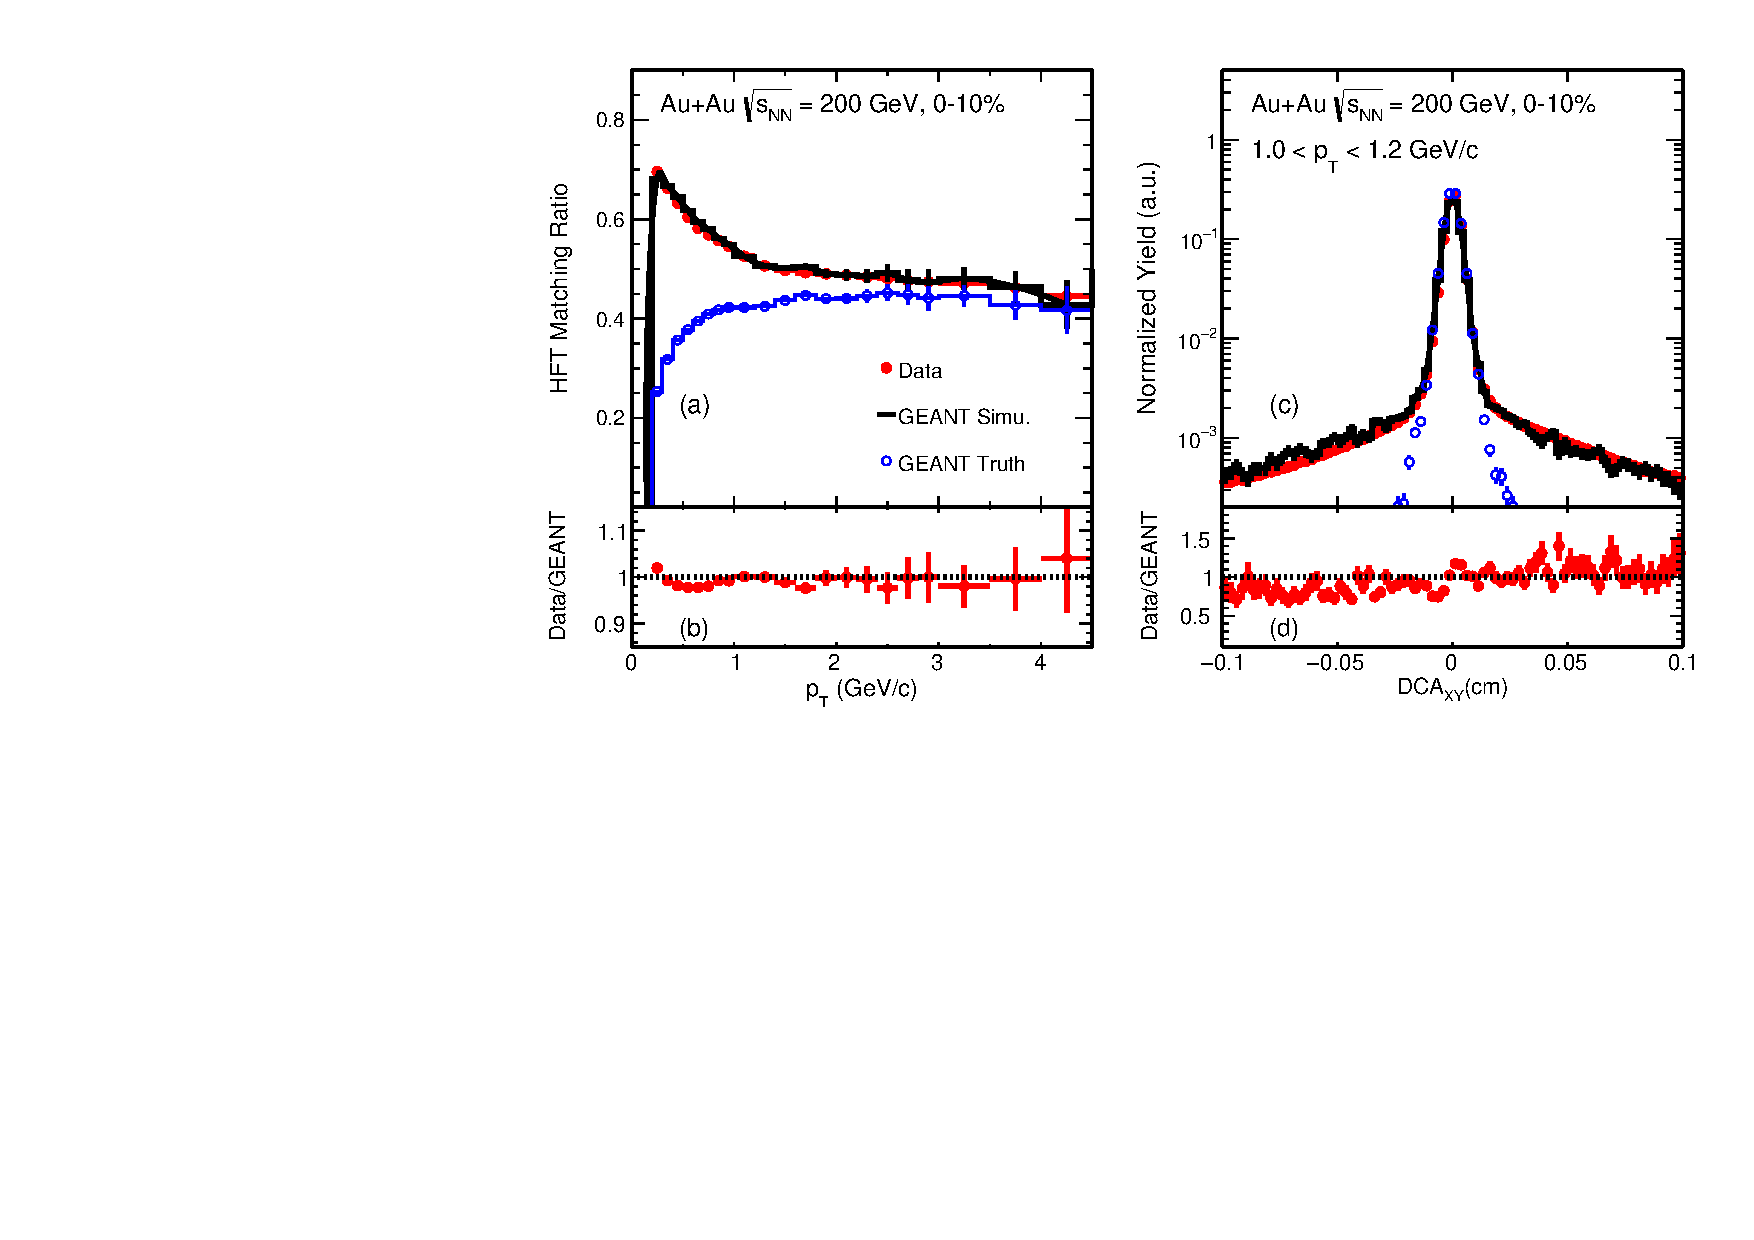
\includegraphics[width=0.85\textwidth]{fig/HijingRatioDca.pdf}
%DIFDELCMD < %%%
%DIFDELCMD < \caption{%
{%DIFAUXCMD
\DIFdelFL{HFT matching ratio (a) and DCA$_{\rm XY}$ (c) distributions of inclusive charged pions from real data and MC simulation in 0--10\% Au+Au collisions at $\sqrt{s_{_{\rm NN}}}$ = 200\,GeV. The ratios between real data and GEANT simulation are shown in the bottom panels. The blue histogram depicts the true matches in the GEANT simulation.}}
%DIFAUXCMD
%DIFDELCMD < %DIFDELCMD < \label{fig:HijingRatioDca} %%%
%DIFDELCMD < \end{figure*}
%DIFDELCMD < 

%DIFDELCMD < %%%
\DIFdelend % Effectively, these 1D and 2D histograms encode HFT efficiency, acceptance and spatial resolution performance in Run14 data.

With the tuned simulation setup (with ideal HFT geometry), we use this sample to validate our data-driven simulation approach for $D^0$ efficiency \DIFdelbegin \DIFdel{correction }\DIFdelend calculation. We follow the same procedure as described in Sec.~\DIFdelbegin \DIFdel{\ref{sec:correction:hft:fastsim} }\DIFdelend \DIFaddbegin \DIFadd{\ref{correction:hft:fastsim} }\DIFaddend to obtain the HFT match ratio as well as the 2D $\textup{DCA}_\textup{XY}$-$\textup{DCA}_\textup{Z}$ distributions \DIFaddbegin \DIFadd{for primary particles }\DIFaddend from the reconstructed data. \DIFdelbegin \DIFdel{They }\DIFdelend \DIFaddbegin \DIFadd{Then the HFT match ratio and 2D DCA distributions }\DIFaddend are fed into the data-driven simulation to calculate the $D^0$ reconstruction efficiency. This will be compared to the real $D^0$ reconstruction efficiency directly obtained from the GEANT simulation sample.


\DIFdelbegin %DIFDELCMD < \begin{figure*}
%DIFDELCMD < \centering
%DIFDELCMD < 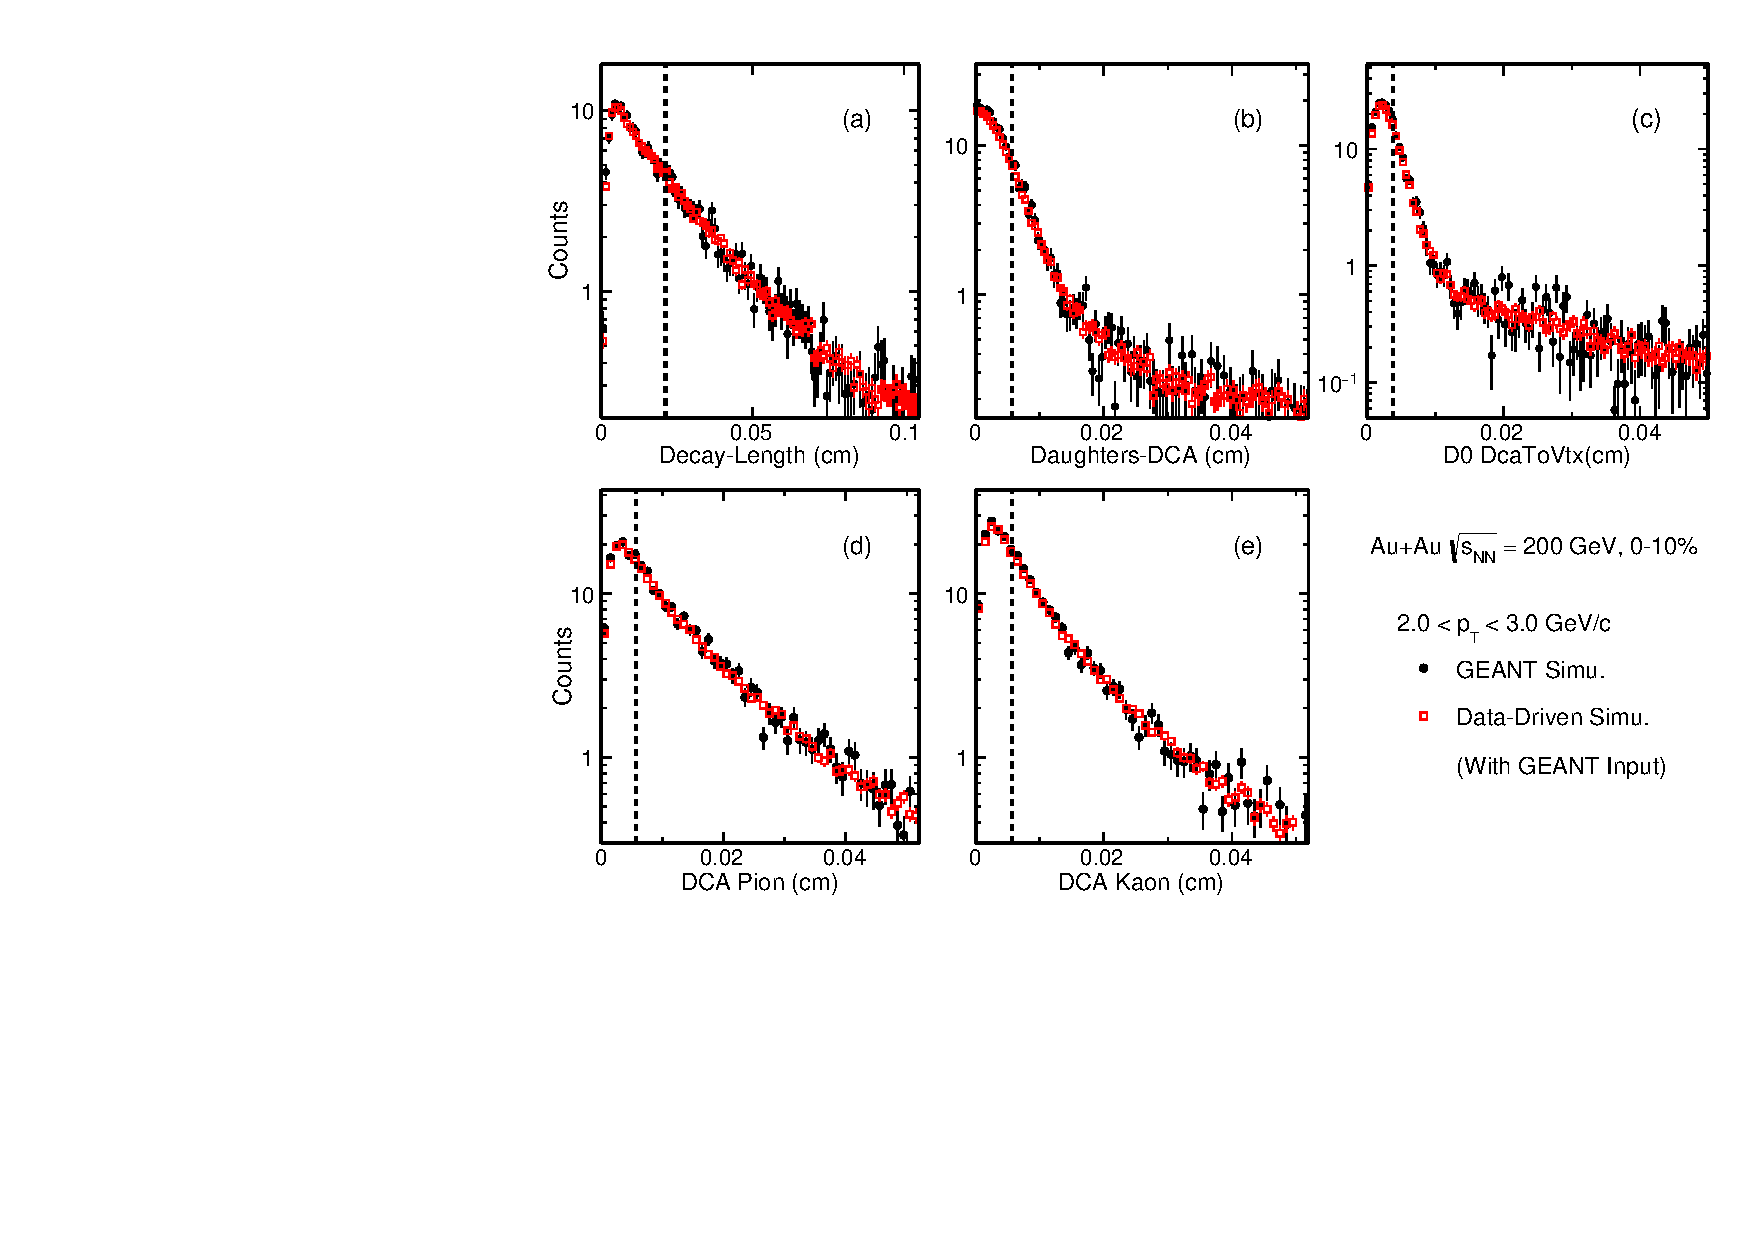
\includegraphics[width=1.0\textwidth]{fig/McTopo.pdf}
%DIFDELCMD < %%%
%DIFDELCMD < \caption{%
{%DIFAUXCMD
\DIFdelFL{Topological distributions comparison between MC GEANT simulation $(black)$ and data-driven fast simulation with the reconstructed distributions in the simulation sample as the input $(red)$ in most central (0--10\%) Au + Au collisions at $\sqrt{s_{_{\rm NN}}}$ = 200\,GeV.}}
%DIFAUXCMD
%DIFDELCMD < %DIFDELCMD < \label{fig:McTopo} %%%
%DIFDELCMD < \end{figure*}
%DIFDELCMD < 

%DIFDELCMD < \begin{figure}
%DIFDELCMD < \centering
%DIFDELCMD < 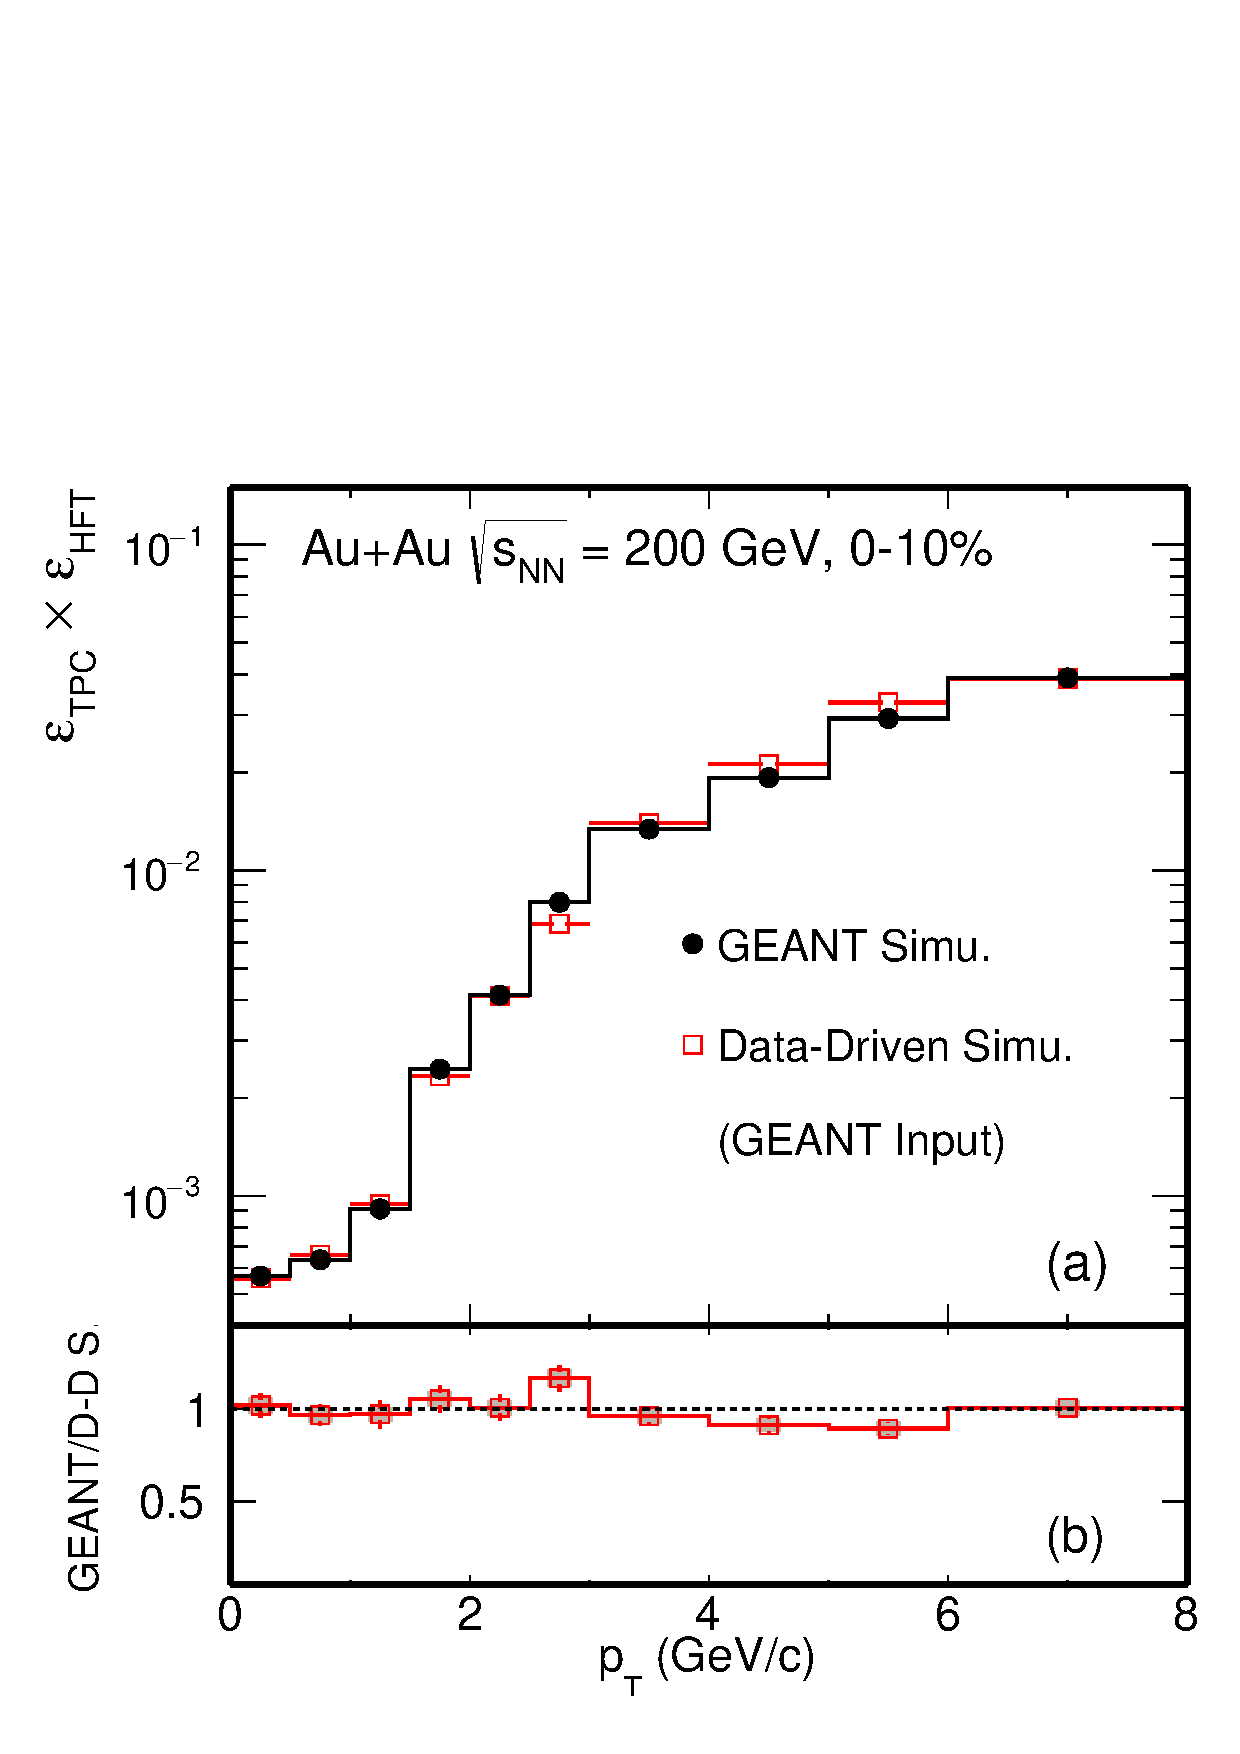
\includegraphics[width=0.43\textwidth]{fig/Mcd0Eff_0_10.pdf}
%DIFDELCMD < %%%
%DIFDELCMD < \caption{%
{%DIFAUXCMD
\DIFdelFL{$D^{0}$ reconstruction efficiency comparison between MC simulation $(black)$ and data-driven fast simulation with the reconstructed distributions in the simulation sample as the input $(red)$ in central 0-10\% Au + Au collisions at $\sqrt{s_{_{\rm NN}}}$ = 200\,GeV.}}
%DIFAUXCMD
%DIFDELCMD < \label{fig:Mcd0Eff_0_10} 
%DIFDELCMD < \end{figure}
%DIFDELCMD < 

%DIFDELCMD < %%%
\DIFdelend %Since the MC simulation can describe the data reasonable well, we can use the simulation samples to verify our efficiency correction procedures. The idea is simple, we have this enriched $D^0$ Hijing simulation sample. After run through the detector and full GEANT simulation, the $D^0$ efficiency and topological variables distributions can be extracted. Another procedure is extract the necessary ingredients from this Hijing simulation sample for the Fast-Simulation input (Fast-Simulation with Hijing input), such as the TPC Tracking efficiency, the HFT matching ratio and the 2D $\textup{DCA}_\textup{XY}$-$\textup{DCA}_\textup{Z}$ distributions similar as we used in real data analysis and discussed in the previous section. Then run through the Fast Simulation, as discussed before, the $D^0$ efficiency and topological variables can also extracted in this way and can be compared to the first Hijing + GEANT procedure.

To validate the data-driven simulation tool, Fig.~\ref{fig:McTopo} shows \DIFaddbegin \DIFadd{an example of the }\DIFaddend comparisons of several topological variables used in the $D^0$ reconstruction obtained from the GEANT simulation directly and from the data-driven simulation with the \DIFdelbegin \DIFdel{reconstructed }\DIFdelend \DIFaddbegin \DIFadd{extract }\DIFaddend distributions from the GEANT simulation as \DIFdelbegin \DIFdel{the }\DIFdelend \DIFaddbegin \DIFadd{an }\DIFaddend input in the most central (0--10\%) centrality and in 2\DIFdelbegin \DIFdel{$<p_{\rm T}<$}\DIFdelend \DIFaddbegin \DIFadd{$<p_{T}<$}\DIFaddend 3\,GeV/$c$. The topological variables shown here are $D^0$ decay length, DCA between two $D^0$ decay daughters, $D^0$ DCA with respect to the collision vertex, pion DCA and kaon DCA with respect to the collision vertex. As seen in this figure, the data-driven simulation tool reproduces all \DIFaddbegin \DIFadd{of }\DIFaddend these topological distributions quite well. \DIFaddbegin \DIFadd{The agreements for the other $p_{T}$ ranges are also quite good.
}\DIFaddend 

Figure~\ref{fig:Mcd0Eff_0_10} shows the $D^0$ reconstruction efficiency \DIFdelbegin \DIFdel{$\varepsilon_{\rm TPC}\times\varepsilon_{\rm HFT}$ from }\DIFdelend \DIFaddbegin \DIFadd{$\varepsilon_{\rm TPC}$ $\times$ $\varepsilon_{\rm HFT}$ calculated with }\DIFaddend the following two methods in this \DIFaddbegin \DIFadd{GEANT }\DIFaddend simulation. The first method is the standard calculation by applying the tracking and topological cuts for reconstructed $D^0$ mesons in \DIFdelbegin \DIFdel{this }\DIFdelend \DIFaddbegin \DIFadd{the }\DIFaddend simulation sample. In the second method, we employ the data-driven simulation method and take the reconstructed distributions from \DIFdelbegin \DIFdel{this }\DIFdelend \DIFaddbegin \DIFadd{the }\DIFaddend simulation sample as \DIFdelbegin \DIFdel{the }\DIFdelend \DIFaddbegin \DIFadd{an }\DIFaddend input and then calculate the $D^0$ reconstruction efficiency in the data-driven simulation framework. In panel (a) of Fig.~\ref{fig:Mcd0Eff_0_10}, efficiencies from two calculation methods agree well in the \DIFdelbegin \DIFdel{$p_{\rm T}$ }\DIFdelend \DIFaddbegin \DIFadd{$p_{T}$ }\DIFaddend bins in central 0--10\% Au+Au collisions\DIFdelbegin \DIFdel{at $\sqrt{s_{_{\rm NN}}}$ = 200\,GeV}\DIFdelend , and the ratio between the two is shown in panel (b). This demonstrates that the data-driven simulation tool can \DIFdelbegin \DIFdel{reproduce well }\DIFdelend \DIFaddbegin \DIFadd{accurately reproduce }\DIFaddend the real $D^0$ reconstruction efficiency in central Au+Au collisions.

% \begin{figure*}
% \centering
% 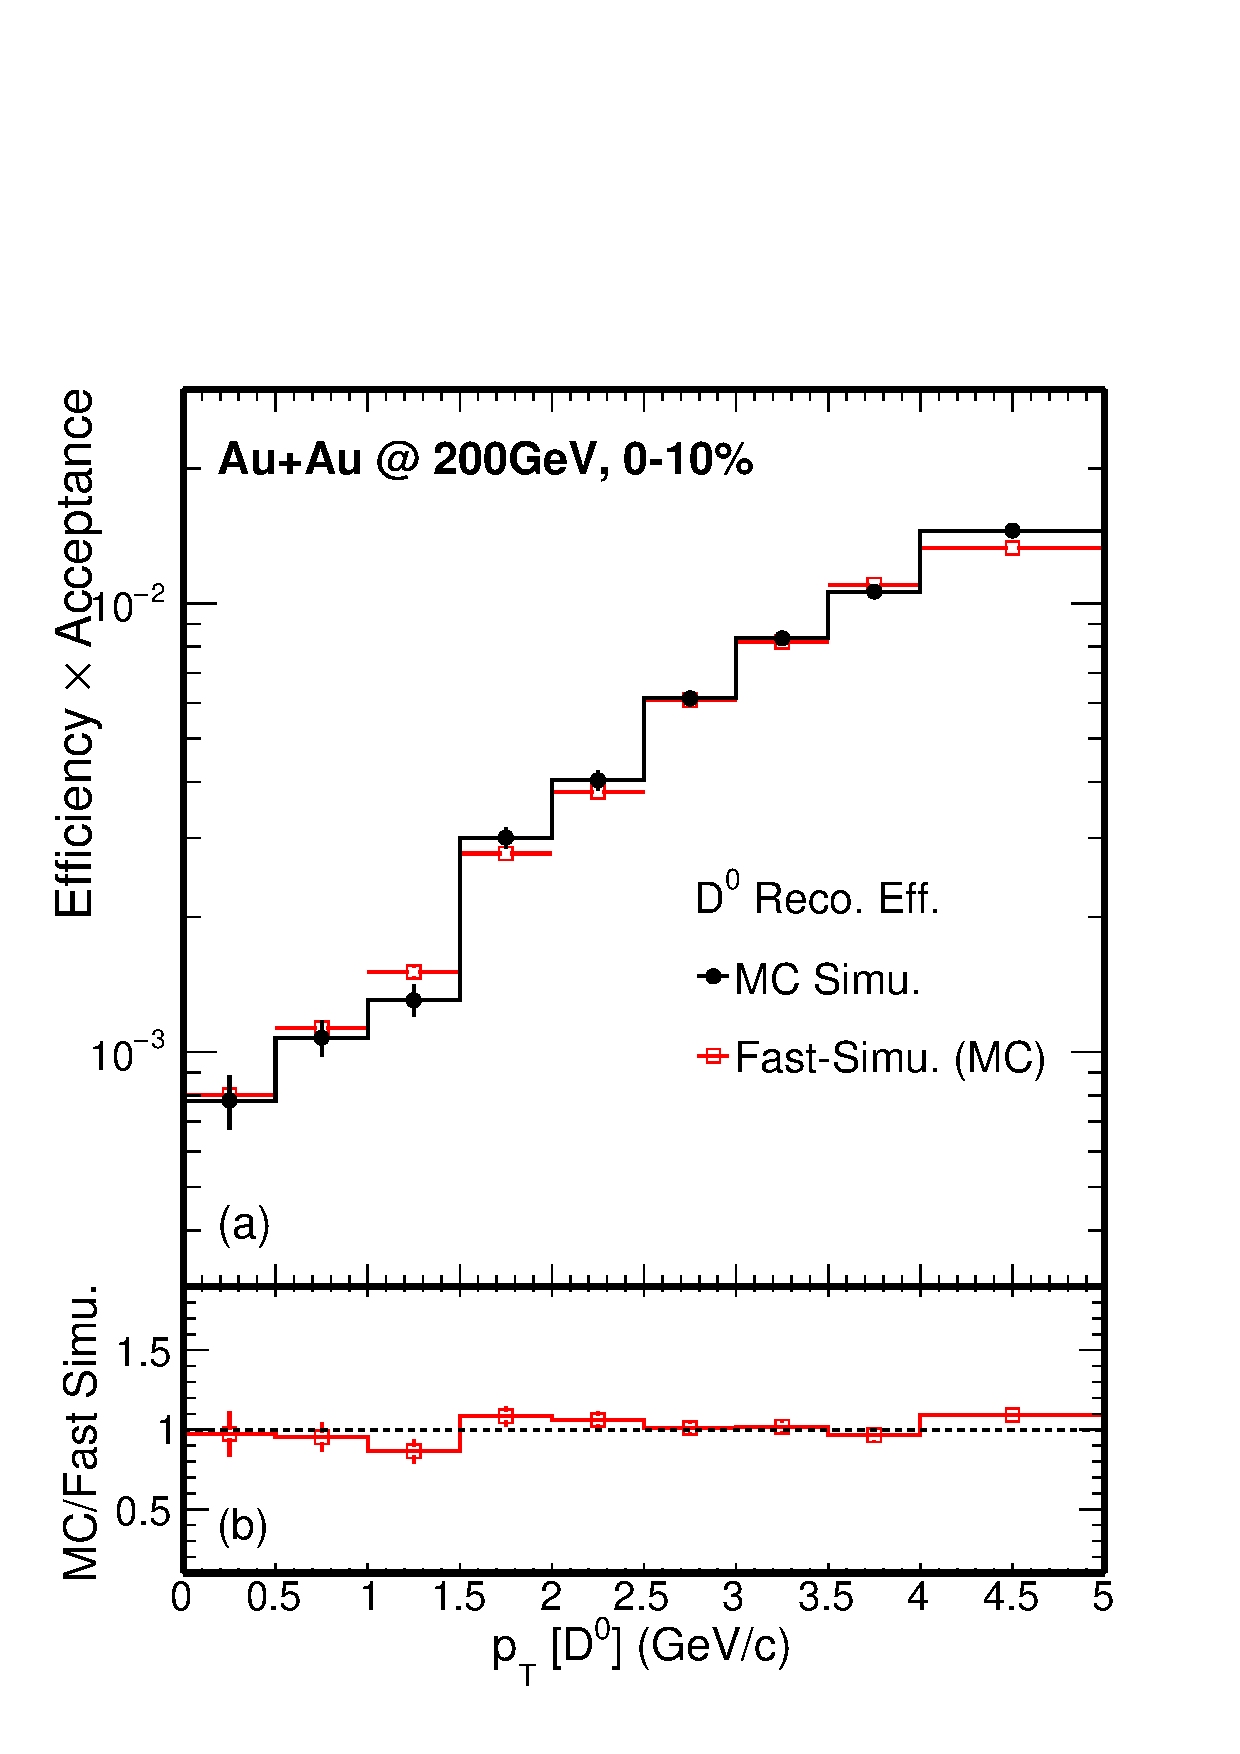
\includegraphics[width=0.45\textwidth]{fig/Mcd0Eff.pdf}
%DIF <  \caption{$D^{0}$ reconstruction efficiency comparison between MC simulation $(black)$ and Fast-Simulation rely on MC simulation as input $(red)$ in most central Au + Au collisions.}
%DIF >  \caption{$D^{0}$ reconstruction efficiency comparison between MC simulation $(black)$ and Fast-Simulation rely on MC simulation as input $(red)$ in most central Au+Au collisions.}
% \label{fig:Mcd0Eff} 
% \end{figure*}

\subsubsection{\DIFdelbegin %DIFDELCMD < %DIFDELCMD < \label{sec:correction:hft:fordata}%%%
%%%
\DIFdelend Efficiency for real data}
\DIFaddbegin \label{correction:hft:fordata}
\DIFaddend 

\begin{figure*}
\centering
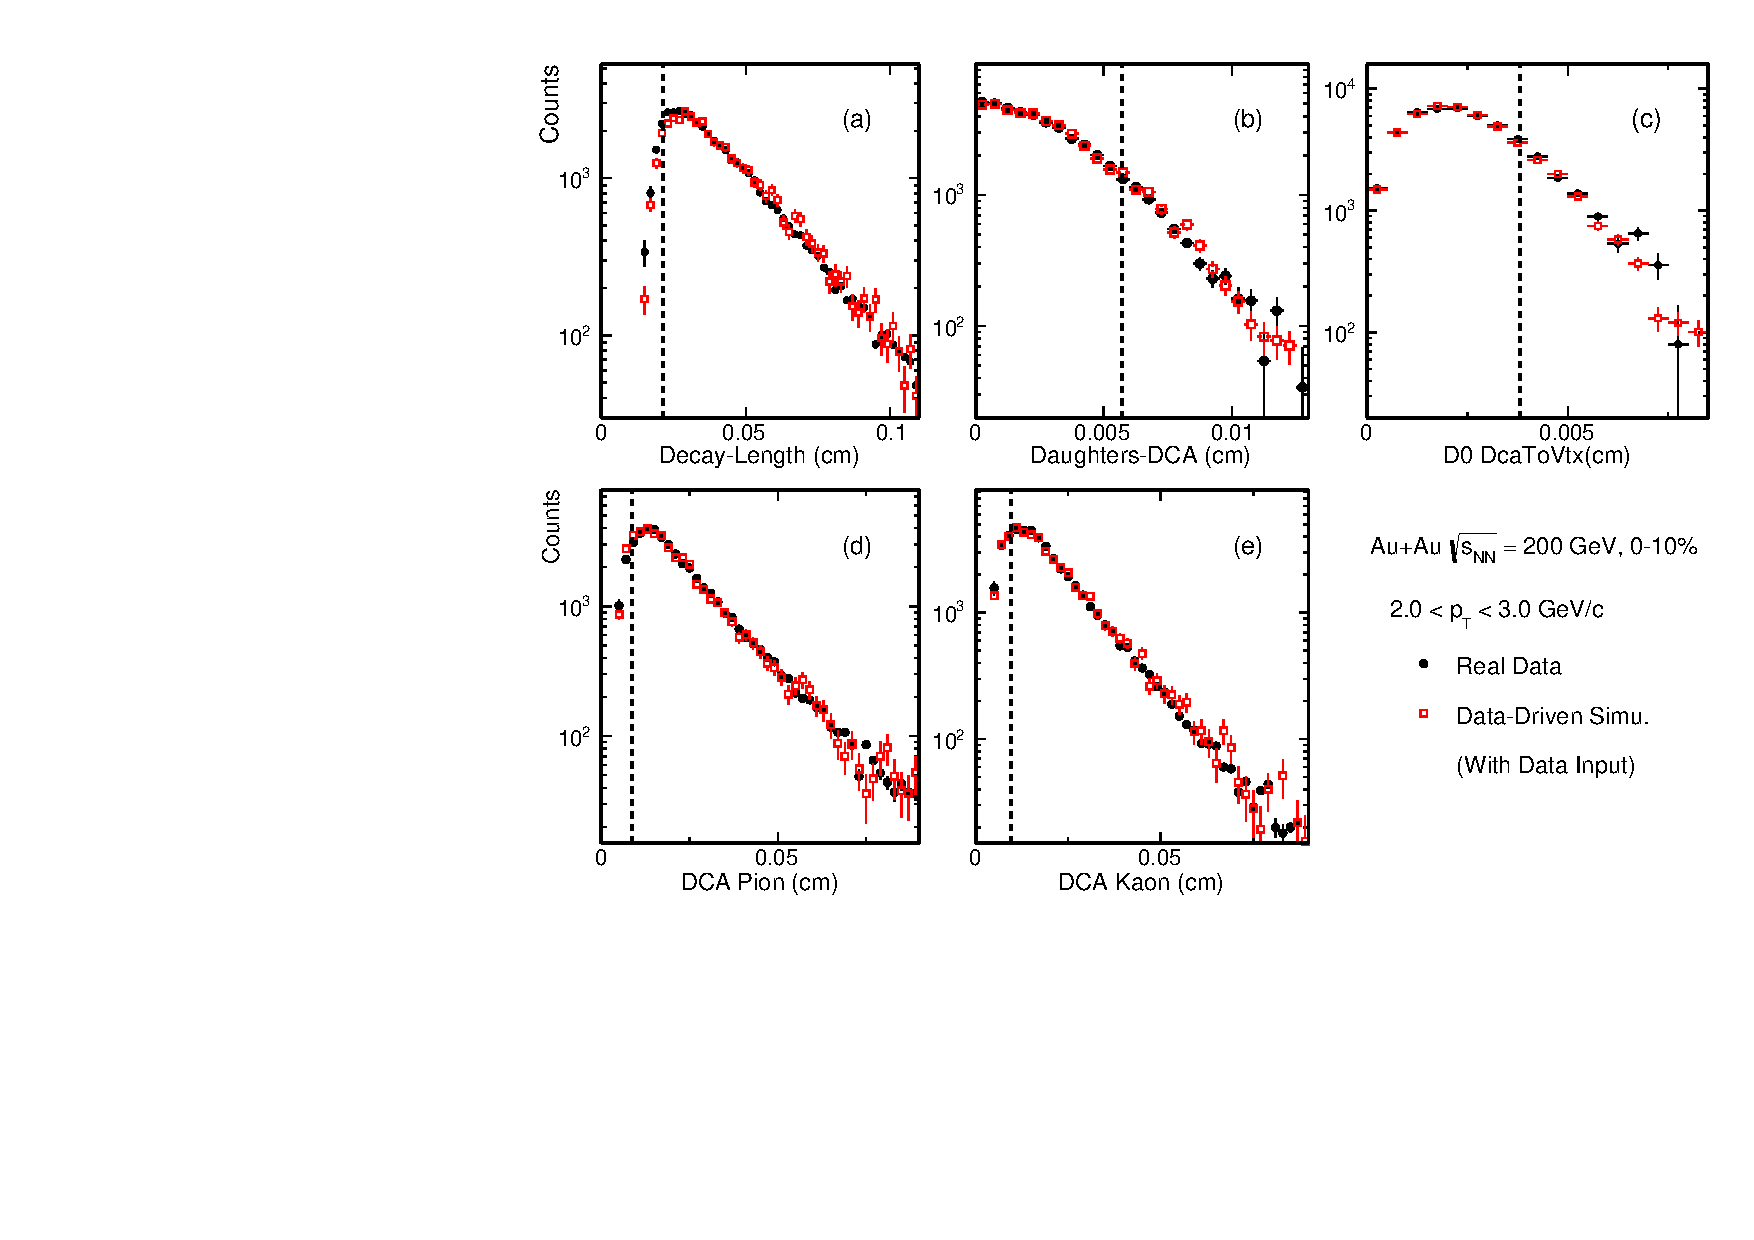
\includegraphics[width=1.0\textwidth]{fig/DataTopo.pdf}
\caption{Comparison of topological variable distributions between $D^0$ signals in real data $(black)$ and in data-driven Simulation with real data distributions as \DIFdelbeginFL \DIFdelFL{the }\DIFdelendFL \DIFaddbeginFL \DIFaddFL{an }\DIFaddendFL input $(red)$ in most central (0--10\%) Au+Au collisions\DIFdelbeginFL \DIFdelFL{at $\sqrt{s_{_{\rm NN}}}$ = 200\,GeV}\DIFdelendFL . The dashed lines indicate the final topological cuts chosen for each individual topological variable.}
\label{fig:DataTopo} 
\end{figure*}

\DIFaddbegin \begin{figure}[h]
\centering
%DIF >  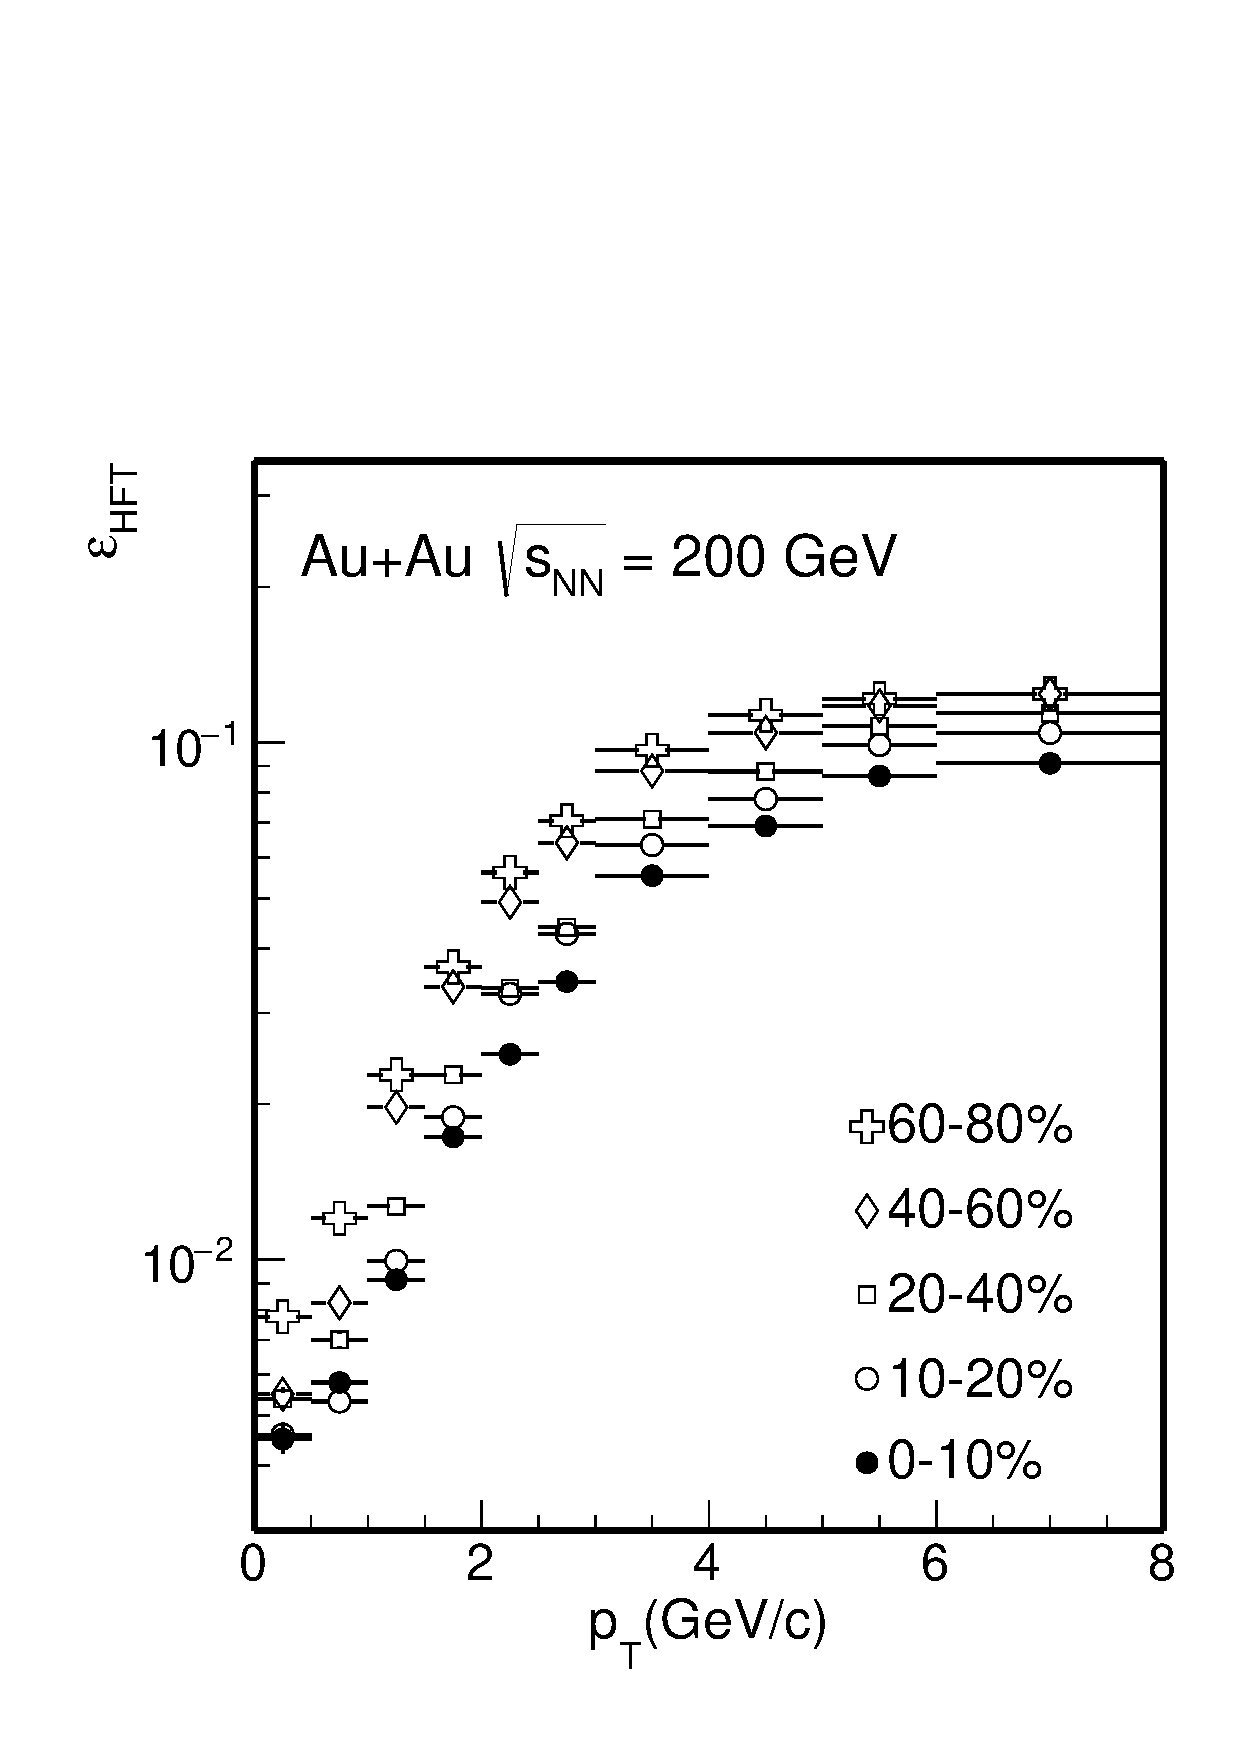
\includegraphics[width=0.4\textwidth]{fig/Datad0Eff_hftTopo.pdf}
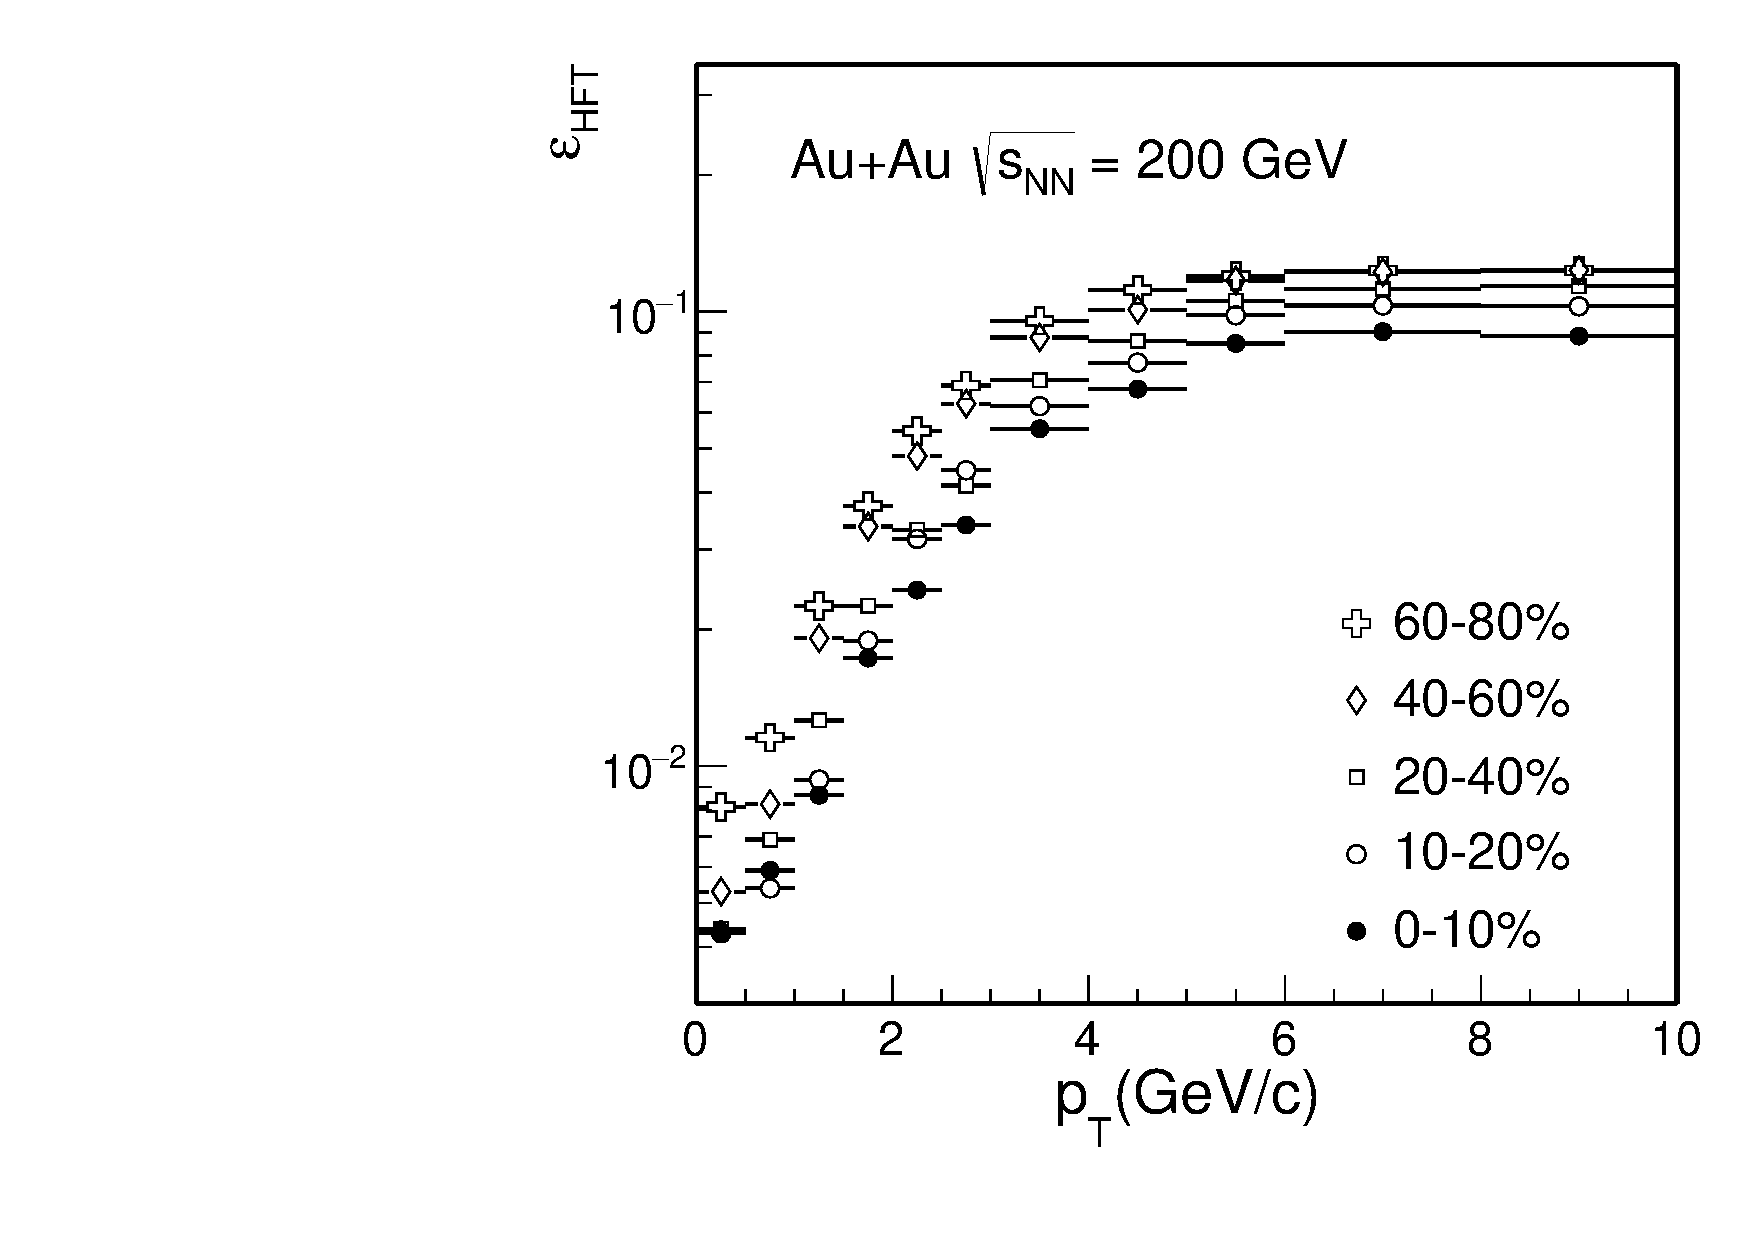
\includegraphics[width=0.43\textwidth]{fig/Datad0Eff_hftTopo_10.pdf}
\caption{\DIFaddFL{$D^{0}$ HFT tracking and topological cut efficiencies from different centrality classes.}}
\label{fig:Datad0Eff_hftTopo} 
\end{figure}



\DIFaddend We employ the validated data-driven simulation method for the real data analysis. \DIFdelbegin \DIFdel{Fig.}\DIFdelend \DIFaddbegin \DIFadd{Figure}\DIFaddend ~\ref{fig:DataTopo} shows the comparisons of the same five topological variables between $D^0$ signals in real data and data-driven simulated distributions with real data as \DIFdelbegin \DIFdel{the }\DIFdelend \DIFaddbegin \DIFadd{an }\DIFaddend input in central 0--10\% collisions for $D^0$ at 2\DIFdelbegin \DIFdel{$<p_{\rm T}<$}\DIFdelend \DIFaddbegin \DIFadd{$<p_{T}<$}\DIFaddend 3\,GeV/$c$. The real data distributions are extracted by reconstructing the $D^0$ signal with initial cuts \DIFaddbegin \DIFadd{(same as the reconstruction cuts in Sec.~\ref{D0recon}, but just remove that particular topological variable as we are going to check) }\DIFaddend and then statistically subtracting the background distributions using the side-band method. The initial cuts are necessary here to ensure reasonable $D^0$ signal reconstruction for the extraction of these topological variable distributions, while these pre-cuts effectively reduce the \DIFdelbegin \DIFdel{low end }\DIFdelend \DIFaddbegin \DIFadd{low-end }\DIFaddend reach for several topological variables, e.g. the $D^0$ decay length. In the data-driven simulation method, charged pion and kaon HFT matching ratio and 2D DCA distributions are used as \DIFdelbegin \DIFdel{the }\DIFdelend \DIFaddbegin \DIFadd{an }\DIFaddend input to calculate these topological variables for $D^0$ signals. \DIFdelbegin \DIFdel{Fig.}\DIFdelend \DIFaddbegin \DIFadd{Figure}\DIFaddend ~\ref{fig:DataTopo} shows that in the selected ranges, the data-driven simulation method reproduces \DIFdelbegin \DIFdel{well }\DIFdelend topological variables distributions of $D^0$ signals, which supports that this method can be reliably used to calculate the topological cut efficiency.


\DIFdelbegin %DIFDELCMD < \begin{figure}[h]
%DIFDELCMD < \centering
%DIFDELCMD < %%%
%DIF <  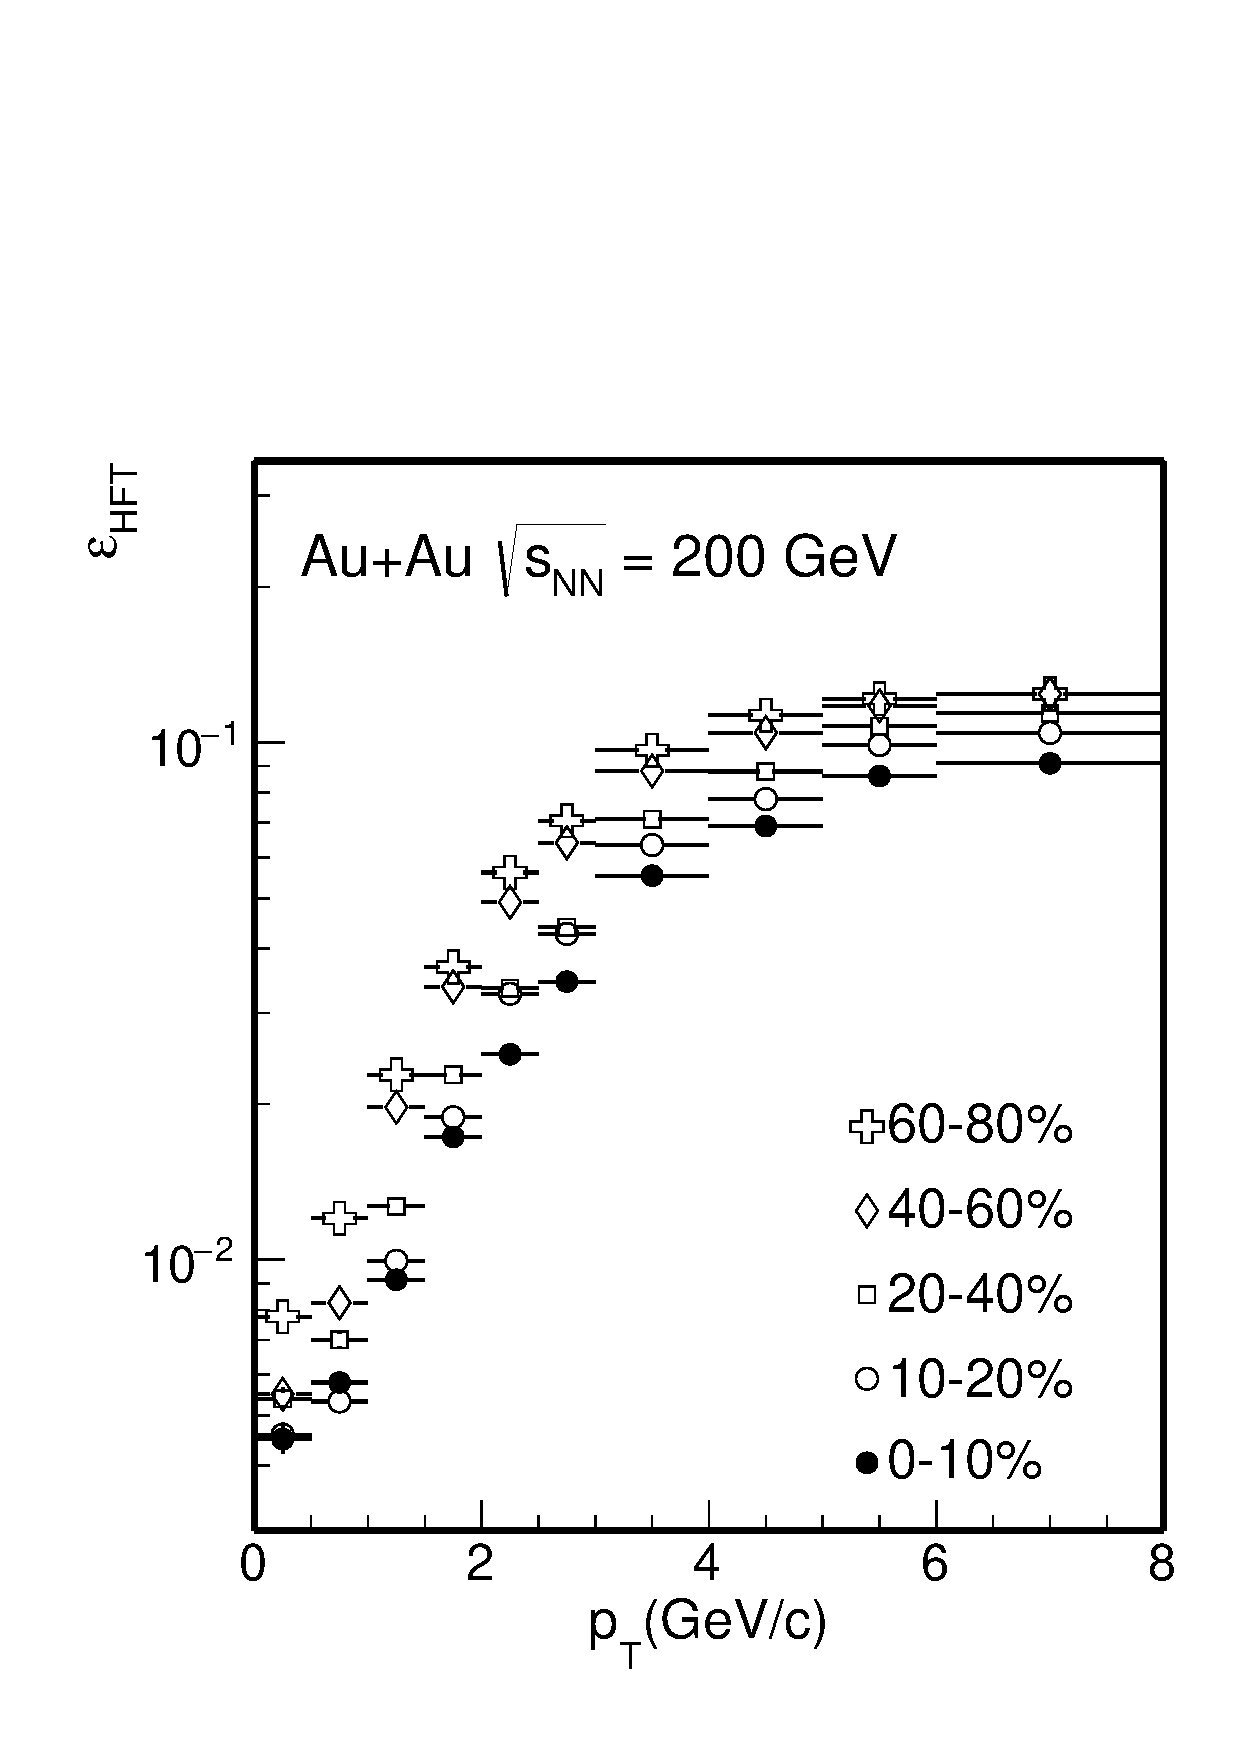
\includegraphics[width=0.4\textwidth]{fig/Datad0Eff_hftTopo.pdf}
%DIFDELCMD < 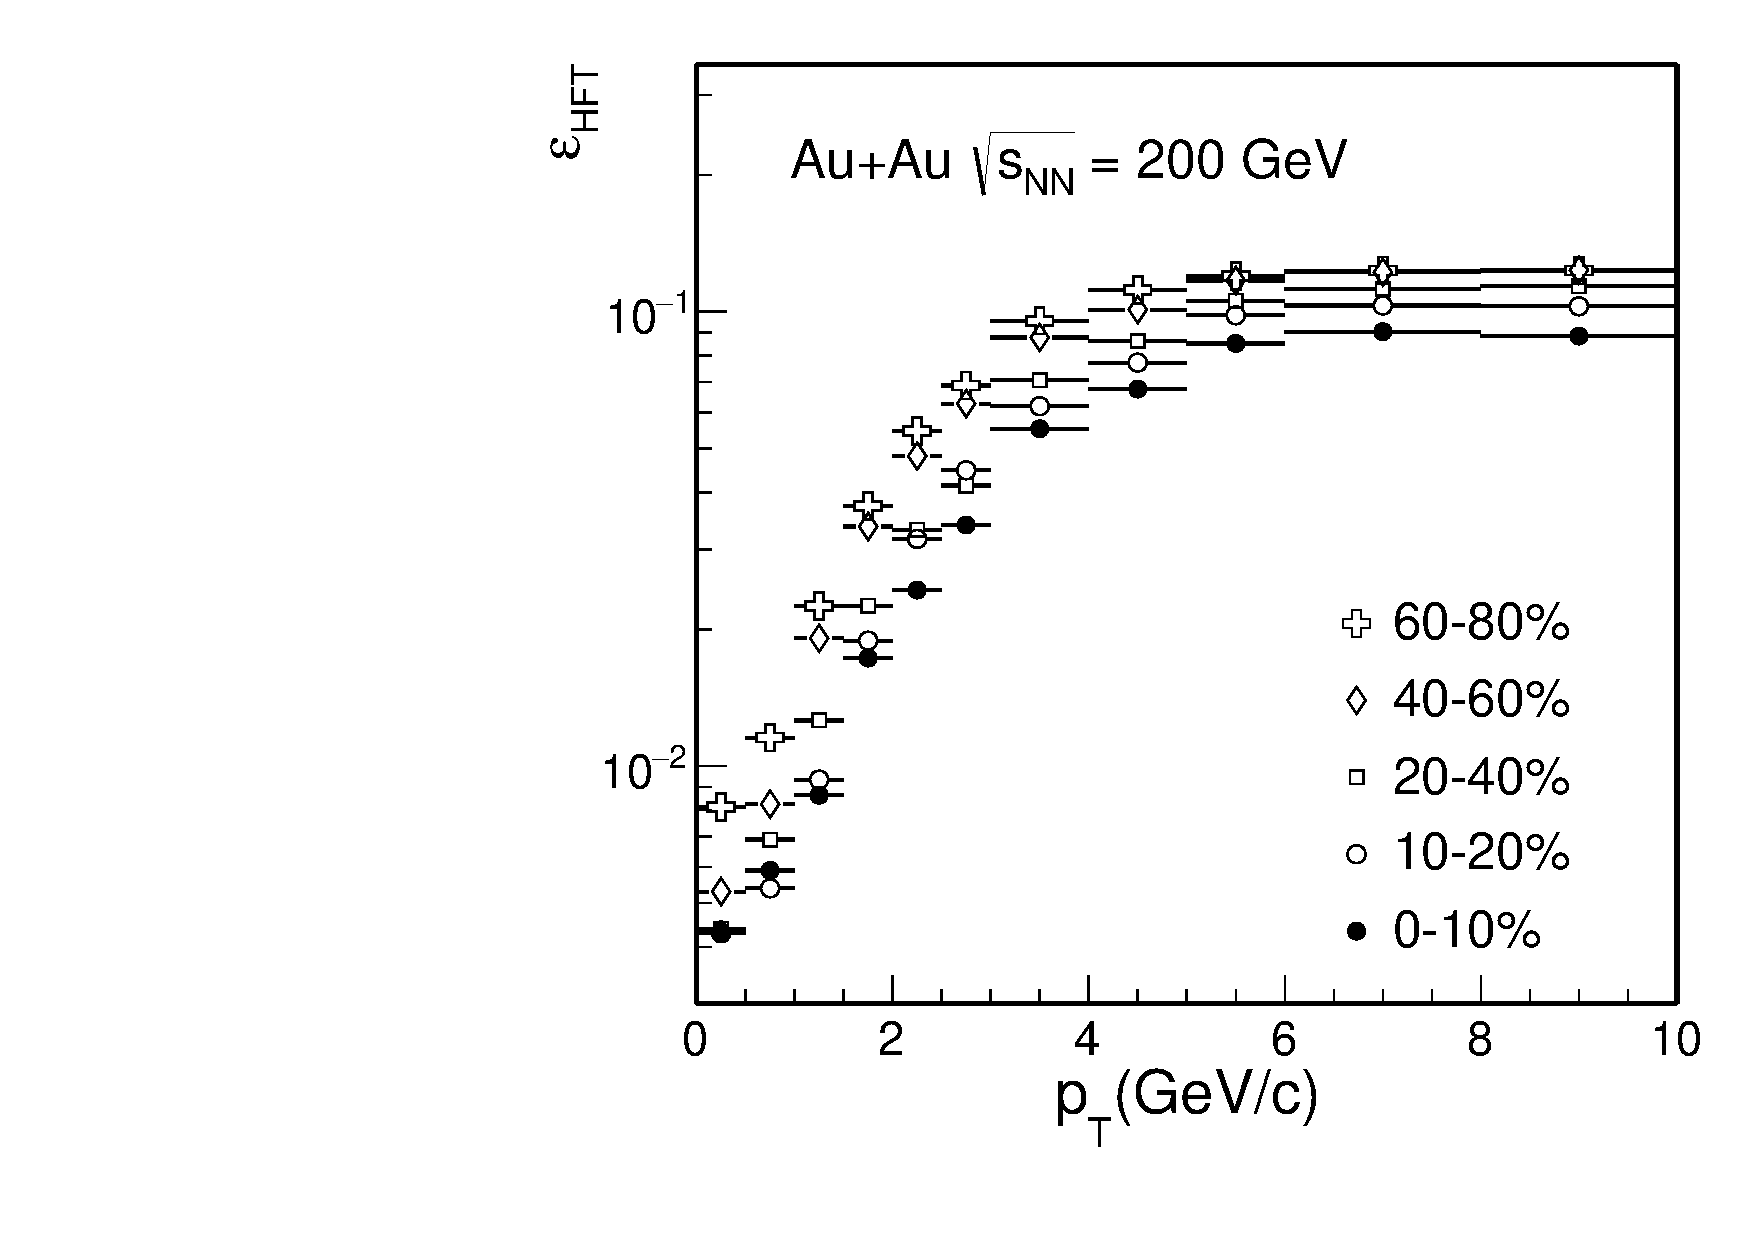
\includegraphics[width=0.43\textwidth]{fig/Datad0Eff_hftTopo_10.pdf}
%DIFDELCMD < %%%
%DIFDELCMD < \caption{%
{%DIFAUXCMD
\DIFdelFL{$D^{0}$ HFT tracking and topological cut efficiencies from different centrality classes in Au + Au collisions at $\sqrt{s_{_{\rm NN}}}$ = 200\,GeV.}}
%DIFAUXCMD
%DIFDELCMD < \label{fig:Datad0Eff_hftTopo} 
%DIFDELCMD < \end{figure}
%DIFDELCMD < 

%DIFDELCMD < %%%
\DIFdelend Figure~\ref{fig:Datad0Eff_hftTopo} shows the HFT tracking and topological cut efficiency $\varepsilon_{\rm HFT}$ as a function of $D^0$ \DIFdelbegin \DIFdel{$p_{\rm T}$ }\DIFdelend \DIFaddbegin \DIFadd{$p_{T}$ }\DIFaddend for different centrality bins obtained using the data-driven simulation method described in this section using the input distributions from \DIFaddbegin \DIFadd{the }\DIFaddend real data. The smaller efficiency seen in central collisions is in part because the HFT tracking efficiency is lower in higher occupancy central collisions, and in addition because we choose tighter topological cuts in central collisions for background suppression.

\subsubsection{\DIFdelbegin %DIFDELCMD < %DIFDELCMD < \label{sec:correction:hft:secondary}%%%
%%%
\DIFdelend Secondary particle contribution}
\DIFaddbegin \label{correction:hft:secondary}
\DIFaddend 

\begin{figure}[h]
\centering
\DIFdelbeginFL %DIFDELCMD < 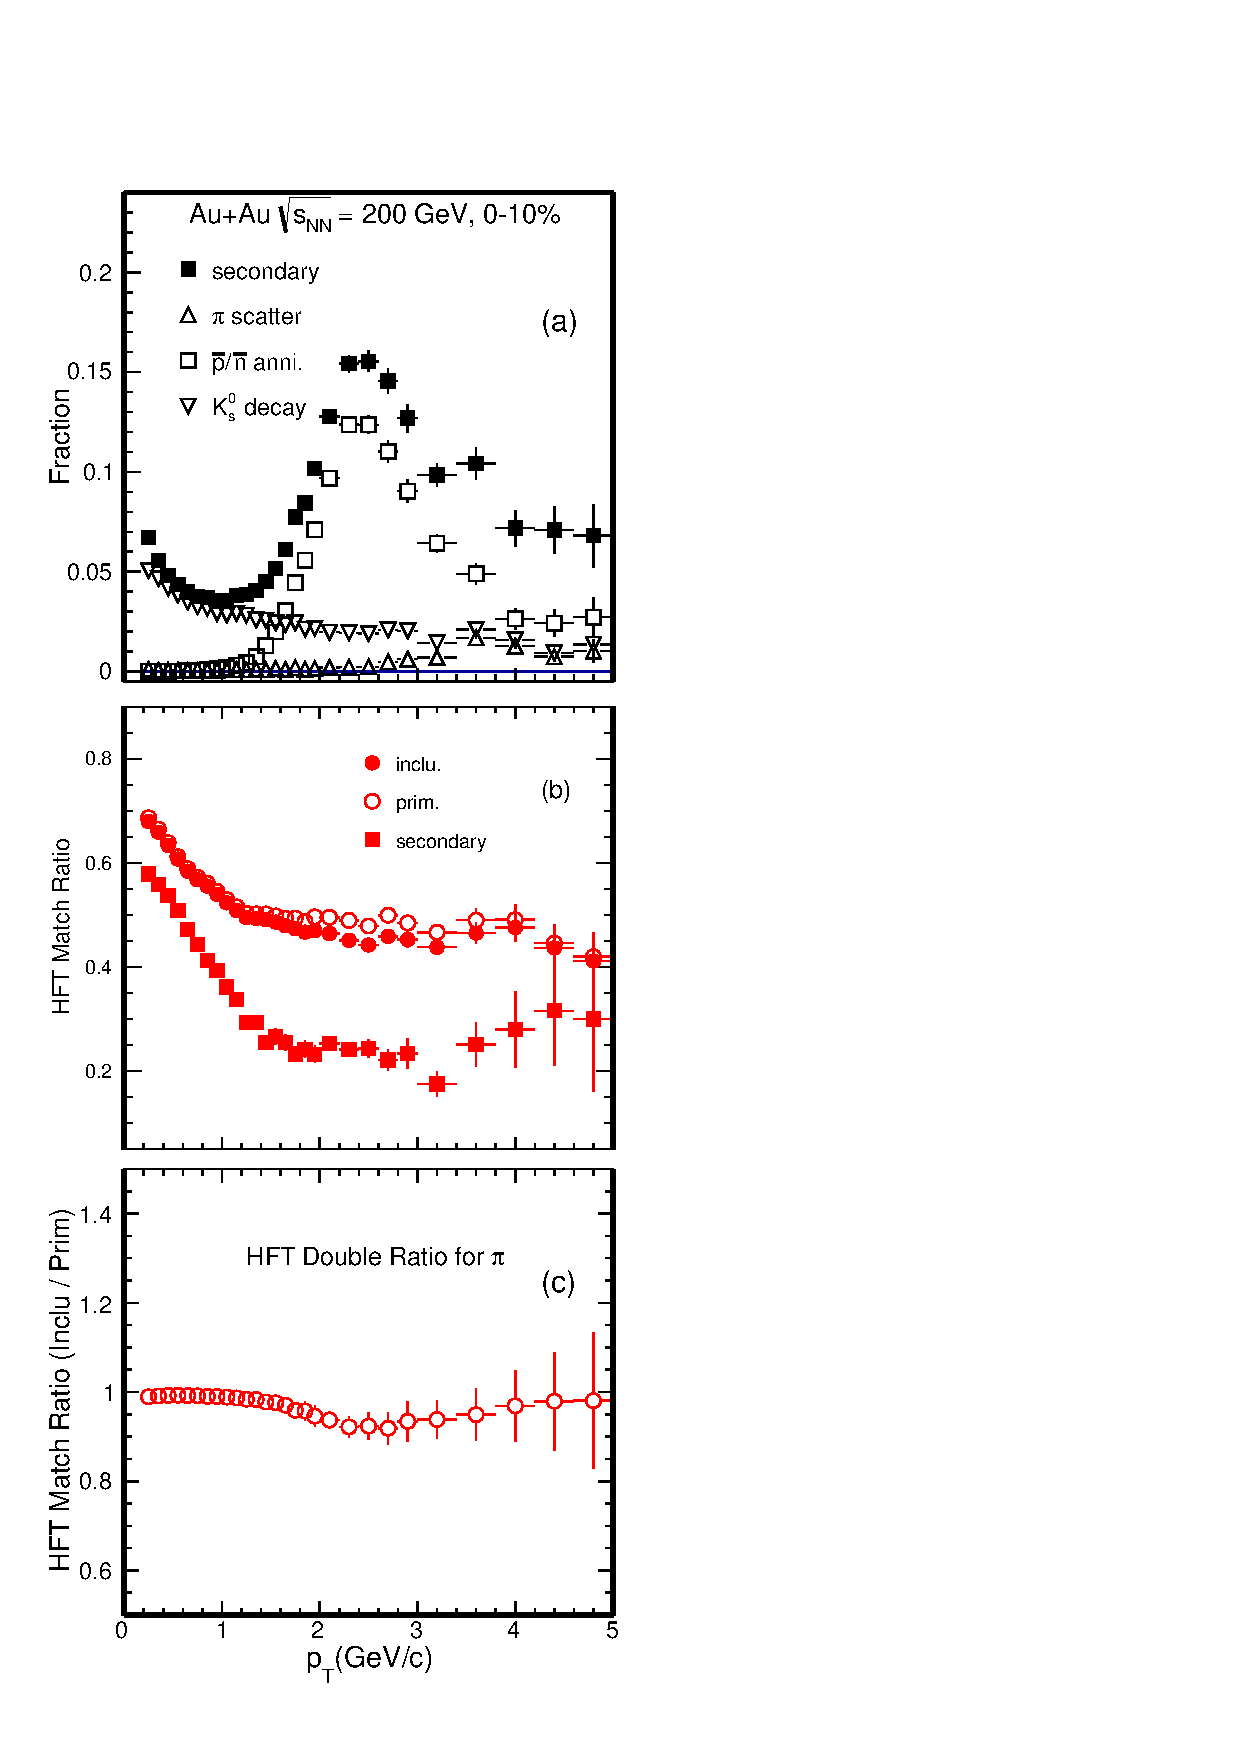
\includegraphics[width=0.41\textwidth, angle = 0]{fig/Fraction_Pion.pdf}
%DIFDELCMD < %%%
\DIFdelendFL \DIFaddbeginFL 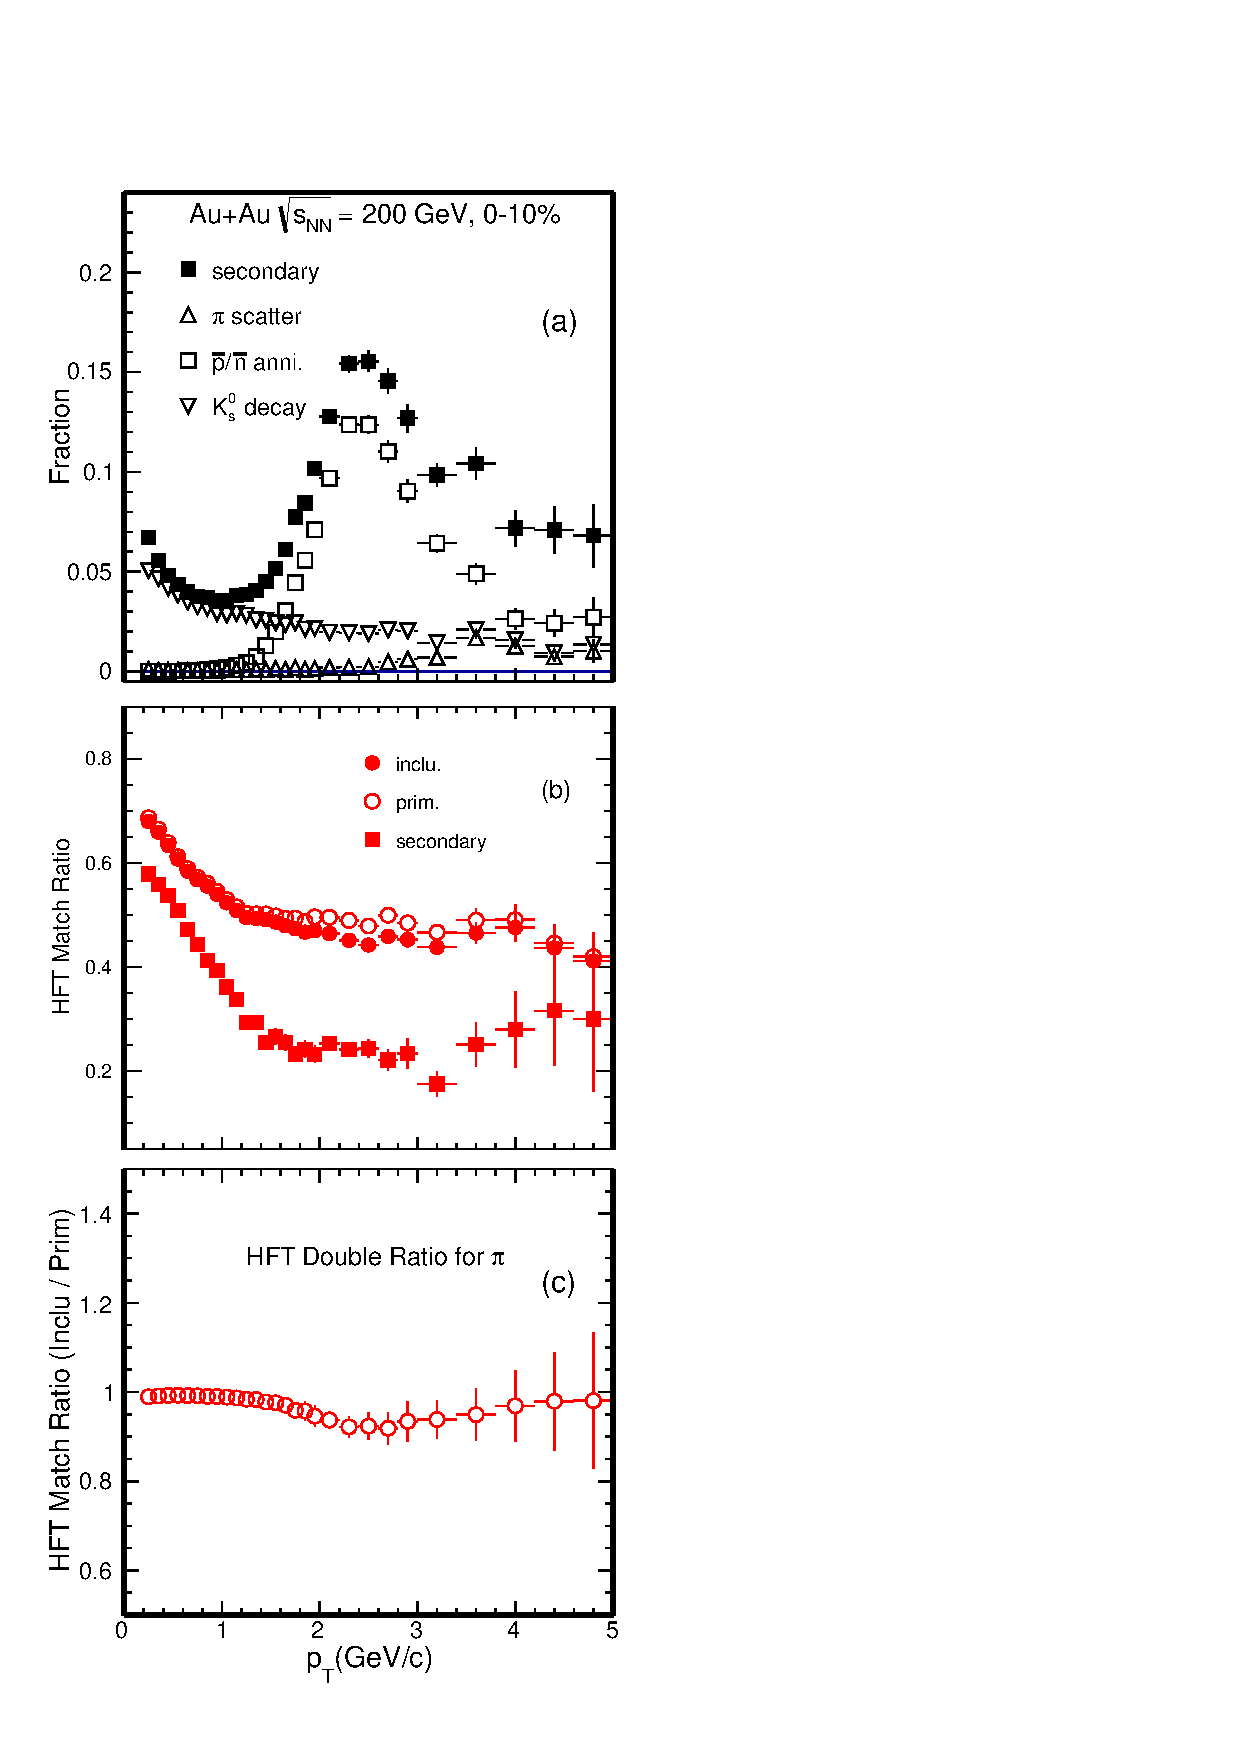
\includegraphics[width=0.39\textwidth, angle = 0]{fig/Fraction_Pion.pdf}
  \DIFaddendFL \caption{Secondary pion contribution\DIFdelbeginFL \DIFdelFL{in Au + Au collisions at $\sqrt{s_{_{\rm NN}}}$ = 200\,GeV}\DIFdelendFL . Panel (a) shows the fraction of different sources for secondary tracks. Panel (b) shows the HFT match ratio while panel (c) shows the HFT match double ratio which divide the inclusive one to the primary \DIFdelbeginFL \DIFdelFL{ones}\DIFdelendFL \DIFaddbeginFL \DIFaddFL{one from panel (b)}\DIFaddendFL .}
\label{fig:Fraction_Pion} 
\end{figure}

\DIFaddbegin \begin{figure}
\centering
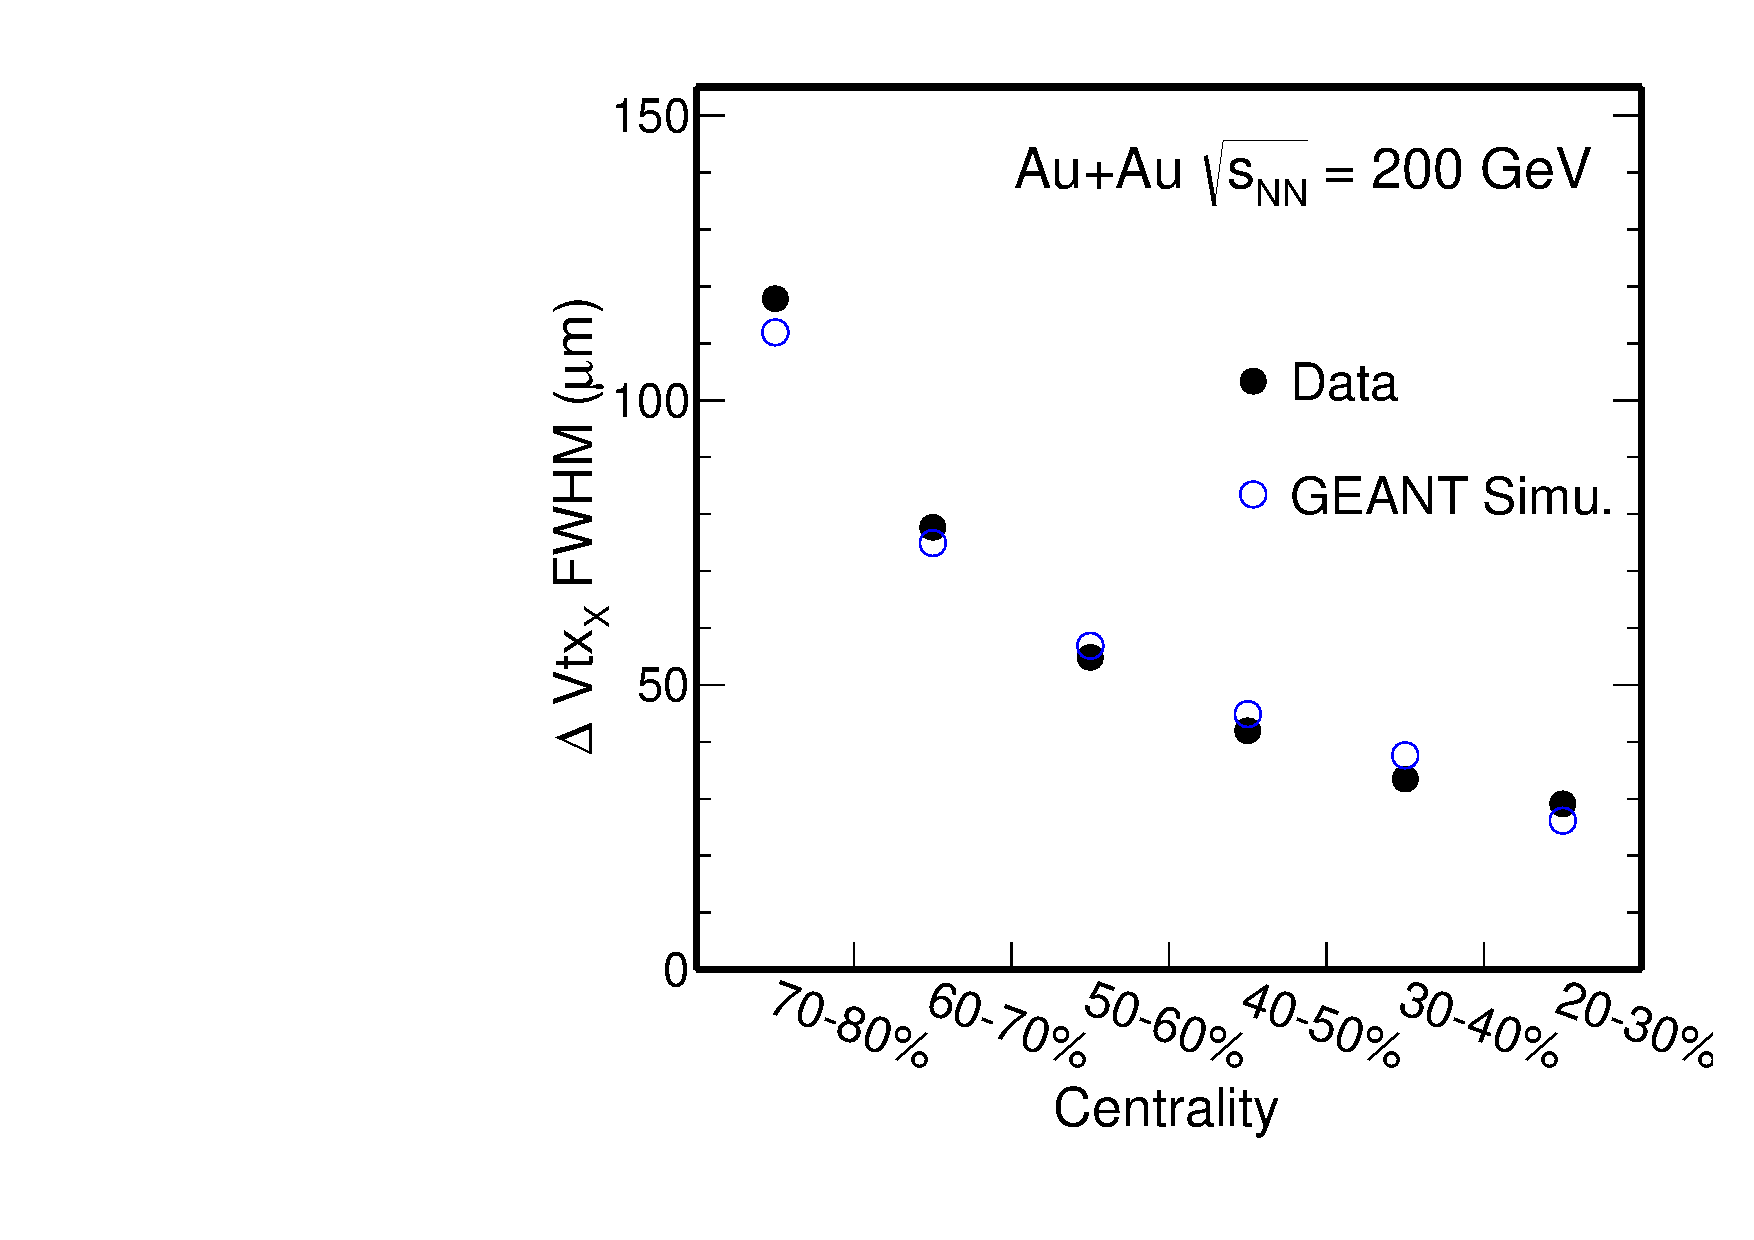
\includegraphics[width=0.41\textwidth]{fig/vtxX_vsCent.pdf}
\caption{\DIFaddFL{Full-Width-at-Half-Maximum (FWHM) of vertex position difference in the X dimension between two randomly-divided sub-events in various centrality bins. Black solid circles present the FWHM from real data while the blue empty circles are GEANT simulation.}}
\label{fig:vtxX_vsCent} 
\end{figure}

\begin{figure*}
\centering
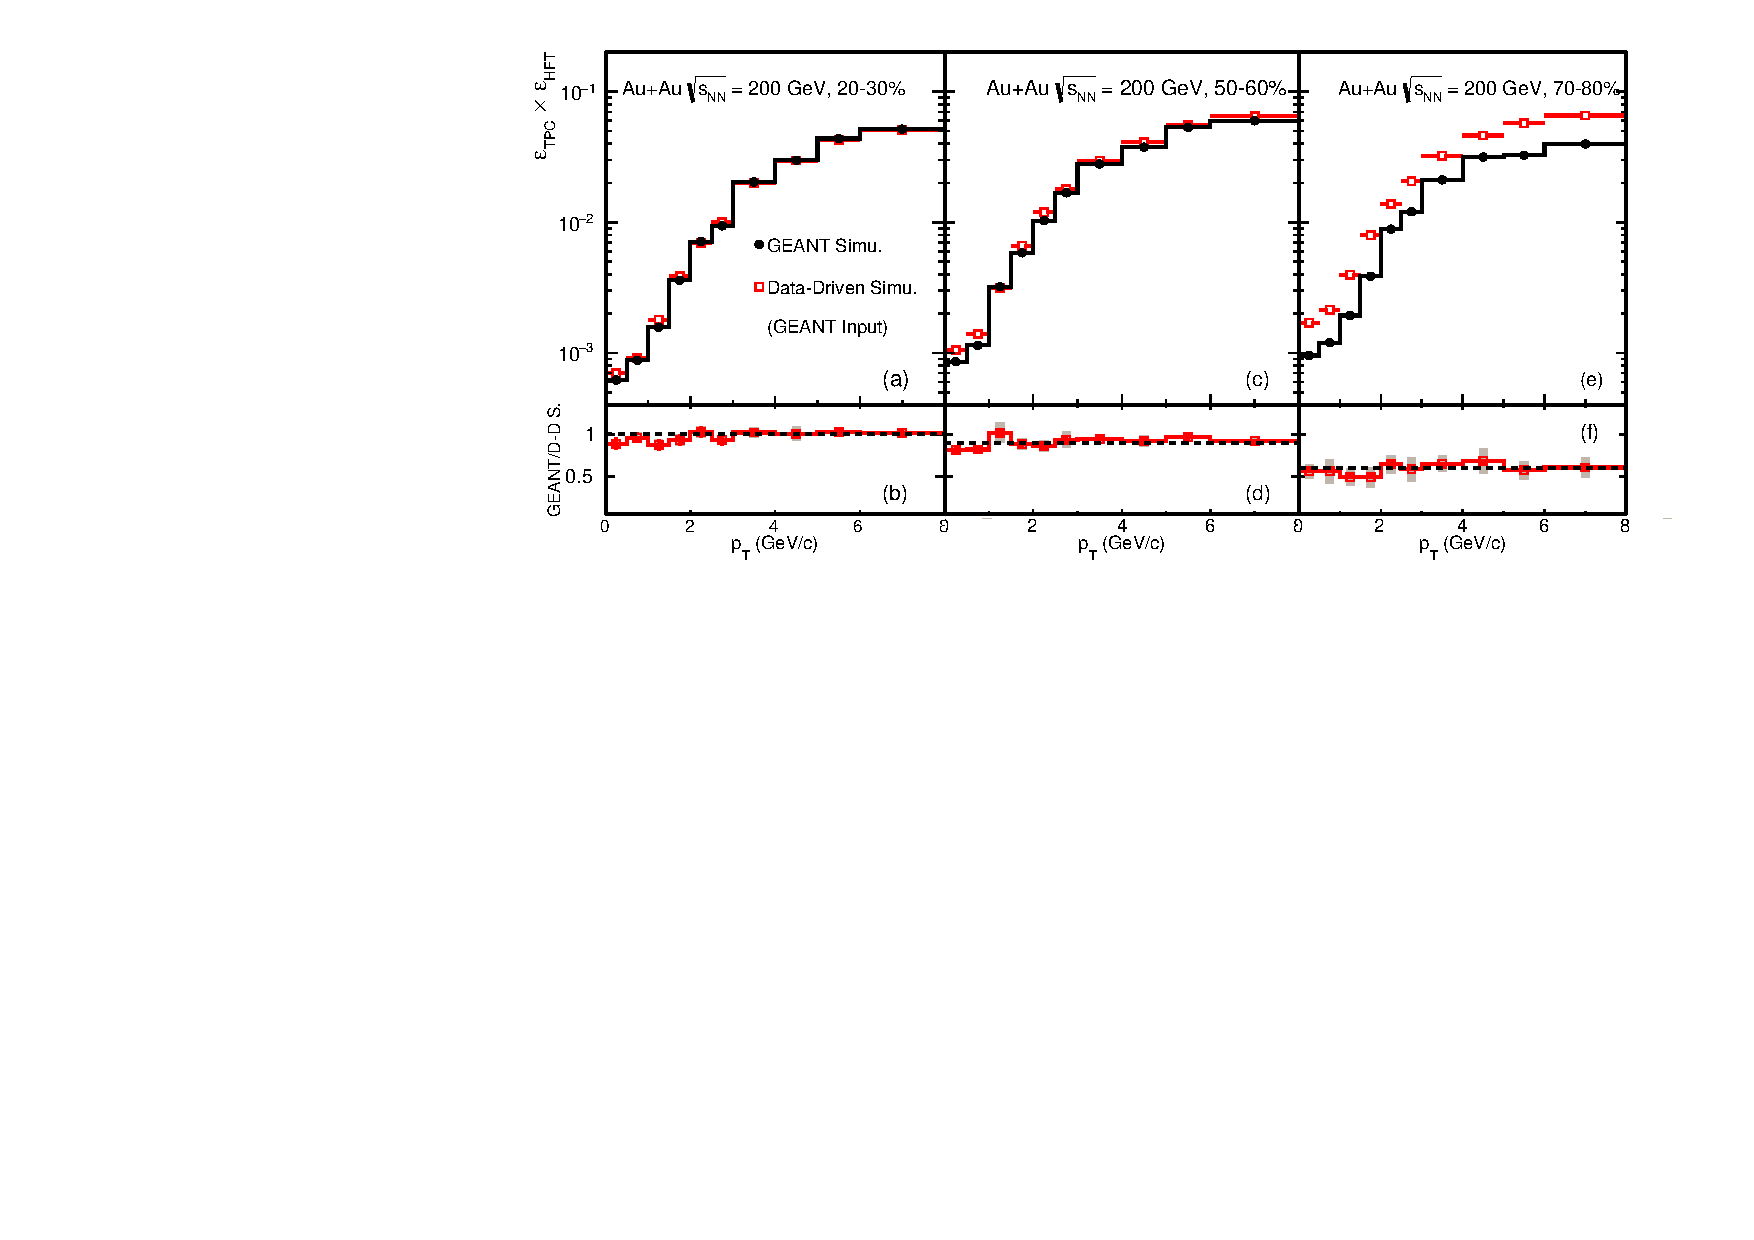
\includegraphics[width=1.05\textwidth]{fig/Mcd0Eff_20_80.pdf}
  \caption{\DIFaddFL{$D^{0}$ reconstruction efficiency comparison between MC GEANT simulation $(black)$ and  data-driven simulation with the reconstructed distributions in the simulation as an input $(red)$ for 20--30\% (a,b), 50--60\% (c,d) and 70--80\% (e,f) Au+Au collisions.}}
\label{fig:Mcd0Eff_20_80} 
\end{figure*}

\DIFaddend In the data-driven method for obtaining the efficiency correction, inclusive pion and kaon distributions are taken from real data as \DIFdelbegin \DIFdel{the input }\DIFdelend \DIFaddbegin \DIFadd{an input while the validation with GEANT simulation is perform with primary particles}\DIFaddend . There is a small amount of secondary contribution (e.g. weak decays from $K^0_S$ and $\Lambda$) to the measured charged pion tracks.

The impact of secondary particle contribution to the charged pions is studied using the \DIFdelbegin \DIFdel{Hijing }\DIFdelend \DIFaddbegin \DIFadd{HIJING }\DIFaddend events processed through the GEANT simulation and the same offline reconstruction. The fraction of secondary pions from weak decay of strange hadrons ($K^0_S$ and $\Lambda$) to the total inclusive charged pions within ${\rm DCA}<$ 1.5\,cm cut is estimated to be around 5\% at pion \DIFdelbegin \DIFdel{$p_{\rm T}$ }\DIFdelend \DIFaddbegin \DIFadd{$p_{T}$ }\DIFaddend = 0.3\,GeV/$c$ and decrease to be $<2\%$ above 2\,GeV/$c$. This is consistent with what \DIFdelbegin \DIFdel{is }\DIFdelend \DIFaddbegin \DIFadd{was }\DIFaddend observed before in measuring the prompt charged pion spectra~\cite{Adams:2003xp}. There is another finite contribution of low momentum anti-protons and anti-neutrons annihilated in the detector material and producing secondary pions. The transverse momenta of these pions are mostly around 2--3\,GeV/$c$ and the fraction of total inclusive pions is $\sim$ 10--12\% at \DIFdelbegin \DIFdel{$p_{\rm T}=$ 2--3}\DIFdelend \DIFaddbegin \DIFadd{$p_{T} =2\textup{-}3$}\DIFaddend \,GeV/$c$ based on this simulation and contribute $\sim$ 5--8\% to the HFT matching ratio. This was obtained using the GEANT with GHEISHA hadronic package. With a different hadronic package, FLUKA, the secondary pion fraction in 2--3\,GeV/$c$ region is significantly reduced \DIFdelbegin \DIFdel{to be }\DIFdelend \DIFaddbegin \DIFadd{and is }\DIFaddend negligible. The difference between the primary pions and the inclusive pions in the HFT matching ratio has been considered as one additional correction factor to take into account these secondary pions in our data-driven simulation method when calculating the efficiency correction, while the maximum difference with respect to the result obtained using the GHEISHA hadronic package is included as the systematic uncertainty for this source. \DIFdelbegin \DIFdel{Fig.}\DIFdelend \DIFaddbegin \DIFadd{Figure}\DIFaddend ~\ref{fig:Fraction_Pion} shows the secondary pion contribution in Au+Au collisions\DIFdelbegin \DIFdel{at $\sqrt{s_{_{\rm NN}}}$ = 200\,GeV}\DIFdelend . Panel (a) shows the fraction of different sources for secondary tracks including the weak decays, the scatters and the \DIFaddbegin \DIFadd{$\bar{p}/\bar{n}$ }\DIFaddend annihilation. Panel (b) shows the different contributions to the HFT match ratio while panel (c) is the HFT match double ratio which divide the inclusive one to the primary \DIFdelbegin \DIFdel{ones}\DIFdelend \DIFaddbegin \DIFadd{one from panel (b)}\DIFaddend . The effect of such secondary contribution to charged kaons is negligible~\cite{Adams:2003xp}.

\subsection{\DIFdelbegin %DIFDELCMD < %DIFDELCMD < \label{sec:correction:vtx}%%%
%%%
\DIFdelend Vertex Resolution Correction - $\varepsilon_{\rm vtx}$}
\DIFaddbegin \label{correction:vtx}
\DIFaddend 

In the data-driven approach, $D^0$ mesons are injected at \DIFdelbegin \DIFdel{event primary }\DIFdelend \DIFaddbegin \DIFadd{the event }\DIFaddend vertex. In the real data, \DIFdelbegin \DIFdel{reconstructed vertex may have }\DIFdelend \DIFaddbegin \DIFadd{the reconstructed vertex has a }\DIFaddend finite resolution with respect to \DIFaddbegin \DIFadd{the }\DIFaddend real collision vertex. This may have \DIFdelbegin \DIFdel{sizable impact }\DIFdelend \DIFaddbegin \DIFadd{a sizable effect }\DIFaddend on the reconstructed $D^0$ signal counts after applying the topological cuts in small multiplicity events where the event vertex resolution \DIFdelbegin \DIFdel{becomes large. Fig.}\DIFdelend \DIFaddbegin \DIFadd{decreases. Figure}\DIFaddend ~\ref{fig:vtxX_vsCent} shows the Full-Width-at-Half-Maximum (FWHM) of the difference in \DIFdelbegin \DIFdel{a }\DIFdelend \DIFaddbegin \DIFadd{the }\DIFaddend vertex x-position of two randomly-divided sub-events in various centrality bins. We choose the FWHM variable here as the distributions are not particularly Gaussian.

\DIFdelbegin %DIFDELCMD < \begin{figure}
%DIFDELCMD < \centering
%DIFDELCMD < 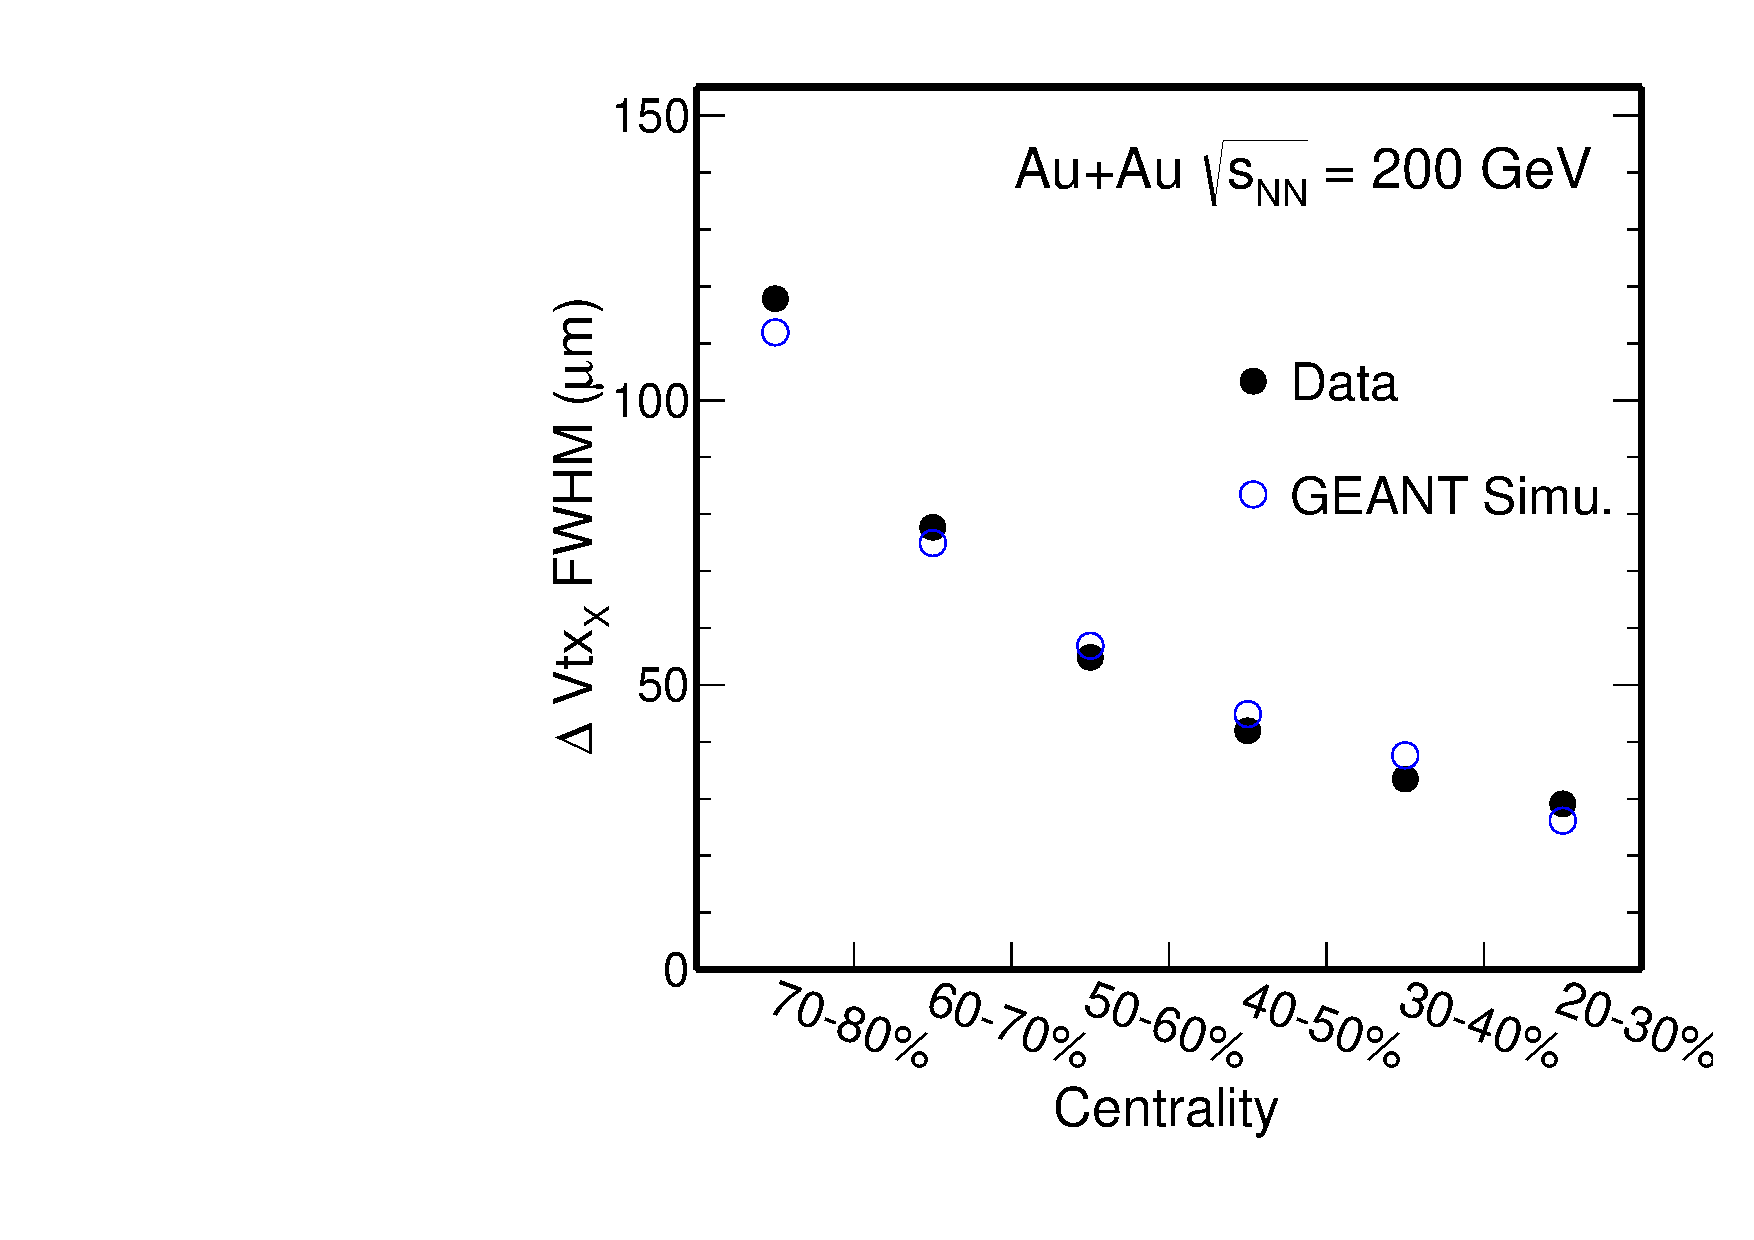
\includegraphics[width=0.41\textwidth]{fig/vtxX_vsCent.pdf}
%DIFDELCMD < %%%
%DIFDELCMD < \caption{%
{%DIFAUXCMD
\DIFdelFL{Full-Width-at-Half-Maximum (FWHM) of vertex position difference in the X dimension between two randomly-divided sub-events in various centrality bins in Au + Au collisions. Black solid circles present the FWHM from real data while the blue empty circles are GEANT simulation.}}
%DIFAUXCMD
%DIFDELCMD < \label{fig:vtxX_vsCent} 
%DIFDELCMD < \end{figure}
%DIFDELCMD < 

%DIFDELCMD < %%%
\DIFdelend The MC simulation reproduces the vertex difference distributions seen in the real data reasonably well. This gives us confidence in using this MC simulation setup to evaluate the vertex resolution correction $\varepsilon_{\rm vtx}$.

\DIFdelbegin %DIFDELCMD < \begin{figure*}
%DIFDELCMD < \centering
%DIFDELCMD < 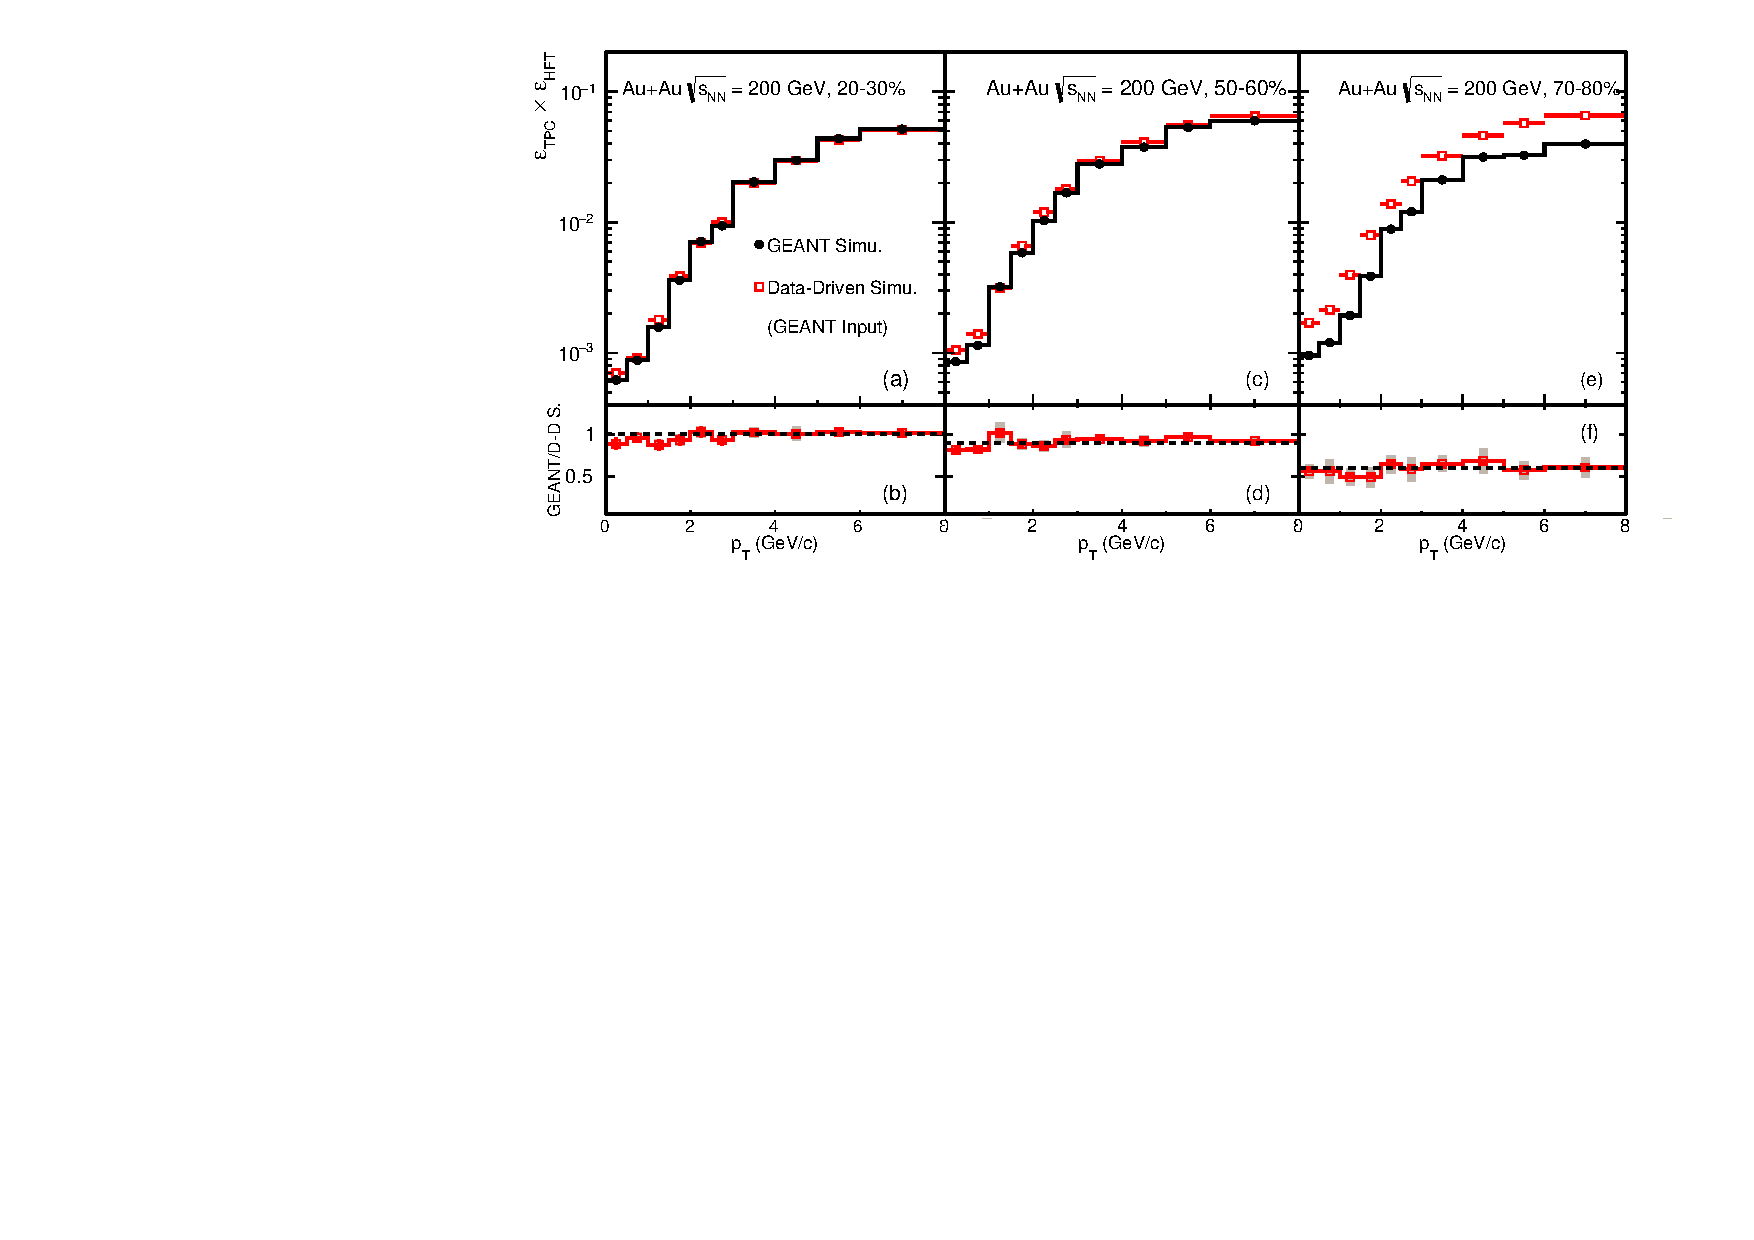
\includegraphics[width=1.05\textwidth]{fig/Mcd0Eff_20_80.pdf}
%DIFDELCMD < %%%
%DIFDELCMD < \caption{%
{%DIFAUXCMD
\DIFdelFL{$D^{0}$ reconstruction efficiency comparison between MC GEANT simulation $(black)$ and  data-driven simulation with the reconstructed distributions in the simulation as the input $(red)$ for 20--30\% (left), 50--60\% (middle) and 70--80\% (right) Au + Au collisions at $\sqrt{s_{_{\rm NN}}}$ = 200\,GeV.}}
%DIFAUXCMD
%DIFDELCMD < \label{fig:Mcd0Eff_20_80} 
%DIFDELCMD < \end{figure*}
%DIFDELCMD < 

%DIFDELCMD < %%%
\DIFdelend \begin{figure}
\centering
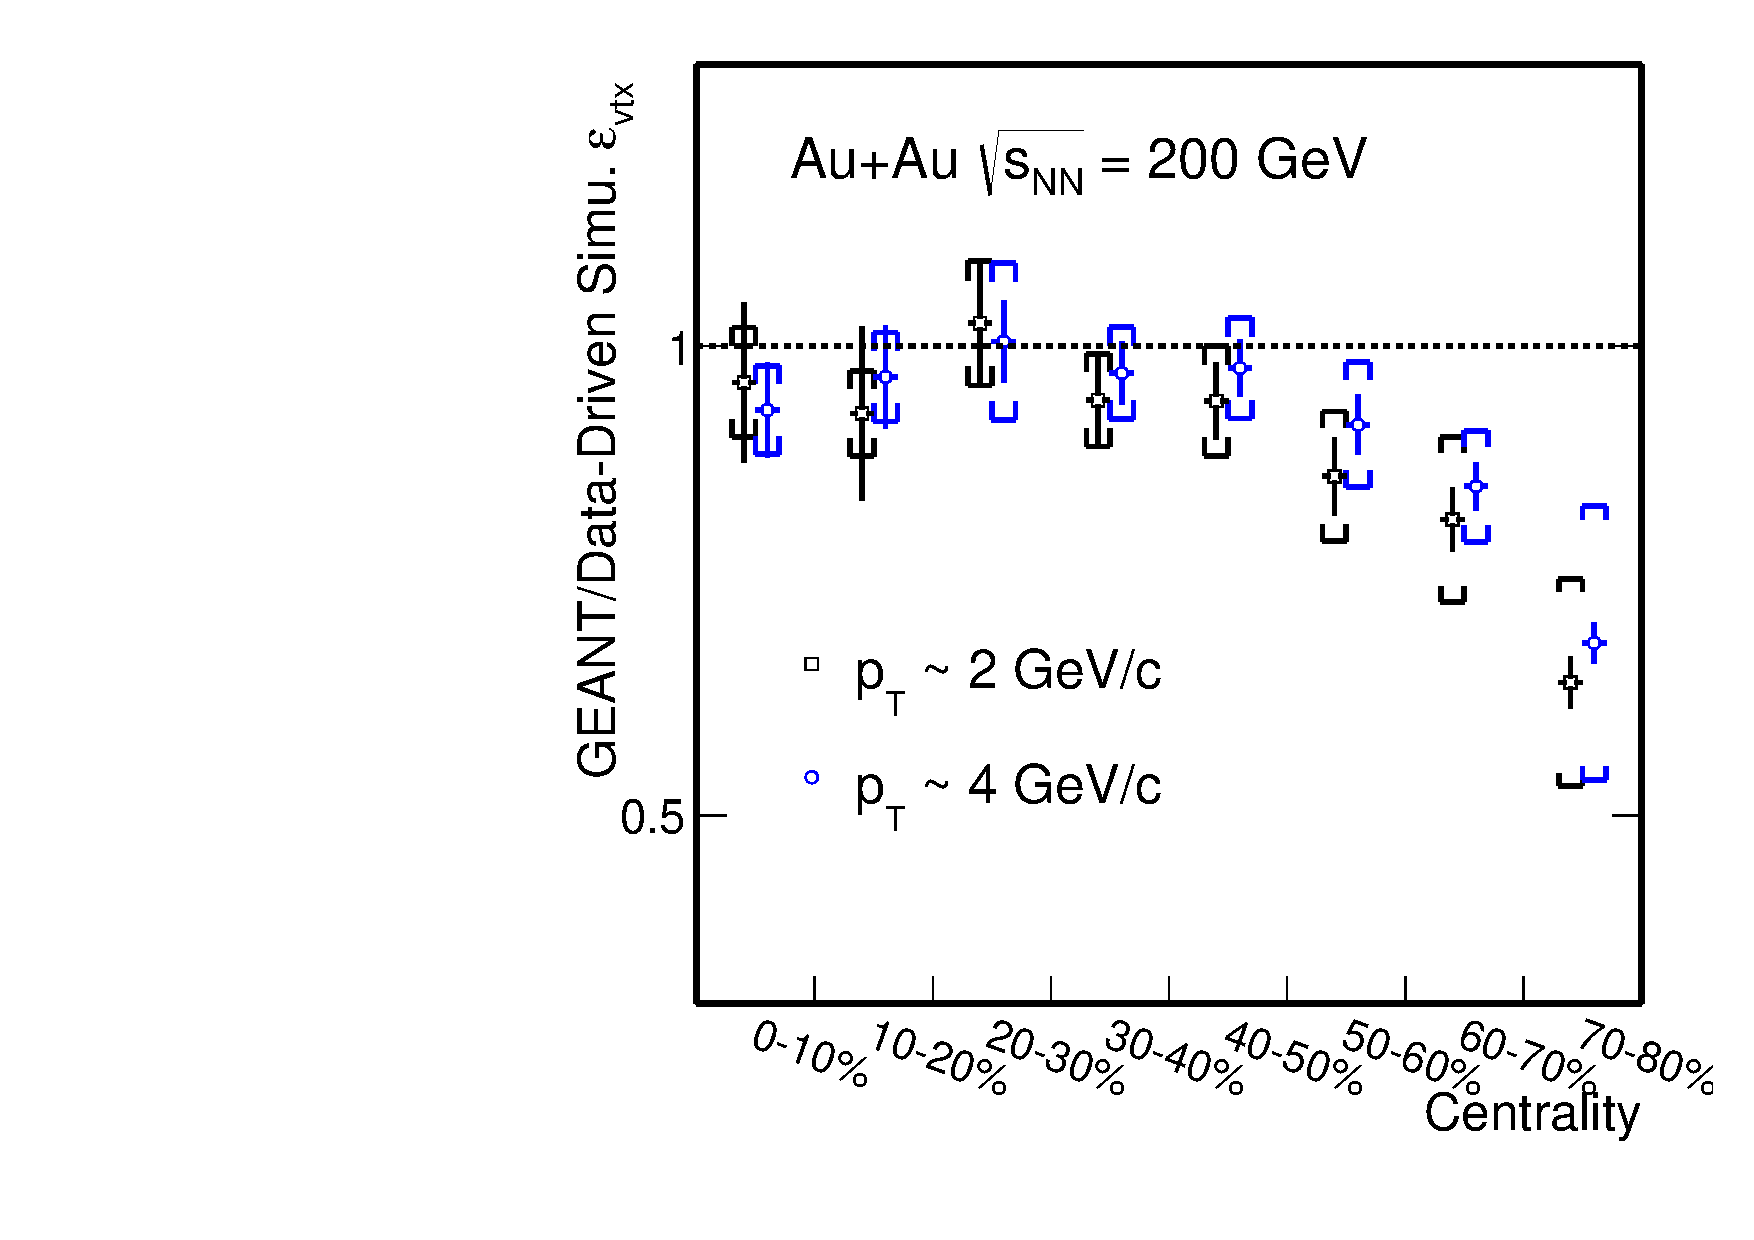
\includegraphics[width=0.43\textwidth]{fig/Mcd0Eff_20_80_vsCent.pdf}
\caption{$\varepsilon_{\rm vtx}$, $D^0$ reconstruction efficiency ratios between MC GEANT simulation and data-driven simulation with the reconstructed distributions in the simulation as \DIFdelbeginFL \DIFdelFL{the }\DIFdelendFL \DIFaddbeginFL \DIFaddFL{an }\DIFaddendFL input versus collision centrality \DIFdelbeginFL \DIFdelFL{in Au + Au collisions }\DIFdelendFL for \DIFdelbeginFL \DIFdelFL{$p_{\rm T}$ }\DIFdelendFL \DIFaddbeginFL \DIFaddFL{$p_{T}$ }\DIFaddendFL at 2 and 4\,GeV/$c$. The brackets depict the estimated systematic uncertainties.}
\label{fig:Mcd0Eff_20_80_vsCent} 
\end{figure}

To estimate the vertex resolution effect, we embedded a PYTHIA $c\bar{c}$ event into a \DIFdelbegin \DIFdel{Hijing }\DIFdelend \DIFaddbegin \DIFadd{HIJING }\DIFaddend Au+Au event, and ran through the STAR GEANT simulation followed by the same offline reconstruction as in the real data production. The PYTHIA $c\bar{c}$ events are pre-selected to have at least one $D^0\rightarrow K^-\pi^+$ decay or its charge conjugate to enhance the statistics. Figure~\ref{fig:Mcd0Eff_20_80} shows the comparison in the obtained $D^0$ reconstruction efficiency between MC simulation $(black)$ and data-driven simulation using reconstructed distributions in the same MC sample as input $(red)$ for 20--30\% (left), 50--60\% (middle) and 70--80\% (right) centrality bins, respectively. The bottom panels show the ratios of the efficiencies obtained from the two calculation methods. In the central and mid-central collisions, the data-driven simulation method can \DIFdelbegin \DIFdel{well }\DIFdelend \DIFaddbegin \DIFadd{properly }\DIFaddend reproduce the $D^0$ real reconstruction efficiency. This is \DIFdelbegin \DIFdel{as }\DIFdelend expected since the vertex resolution is small \DIFaddbegin \DIFadd{enough }\DIFaddend so that it has less impact in the obtained efficiency using the data-driven simulation method. However, in more peripheral collisions, the data-driven simulation method \DIFdelbegin \DIFdel{underestimates }\DIFdelend \DIFaddbegin \DIFadd{overestimates }\DIFaddend the $D^0$ reconstruction efficiency as shown in the middle and right panels. The \DIFdelbegin \DIFdel{ratio between the two methods, the }\DIFdelend vertex resolution correction factor $\varepsilon_{\rm vtx}$\DIFdelbegin \DIFdel{denoted }\DIFdelend \DIFaddbegin \DIFadd{, denotes }\DIFaddend in Equ.~\ref{equ:invariantyield}, has a mild \DIFdelbegin \DIFdel{$p_{\rm T}$ dependence , but shows a }\DIFdelend \DIFaddbegin \DIFadd{$p_{T}$ (2 and 4 GeV/$c$) dependence but }\DIFaddend strong centrality dependence \DIFdelbegin \DIFdel{shown }\DIFdelend in Fig.~\ref{fig:Mcd0Eff_20_80_vsCent}\DIFdelbegin \DIFdel{, which is the $\varepsilon_{\rm vtx}$ correction factor along different centralities for $p_T$ around 2 and 4 GeV/$c$}\DIFdelend . The brackets denote the systematic uncertainties in the obtained correction factor $\varepsilon_{\rm vtx}$. They are estimated by \DIFdelbegin \DIFdel{tuning the Hijing }\DIFdelend \DIFaddbegin \DIFadd{varying the multiplicity range for the HIJING }\DIFaddend + GEANT simulation so that the sub-event vertex difference distributions in the real data can be covered by distributions obtained from different simulation samples. The vertex resolution corrections are applied \DIFaddbegin \DIFadd{as a function of $p_{T}$ }\DIFaddend in each individual \DIFdelbegin \DIFdel{centralities along with the $p_T$ dependence}\DIFdelend \DIFaddbegin \DIFadd{centrality class}\DIFaddend .

\subsection{\DIFdelbegin %DIFDELCMD < %DIFDELCMD < \label{sec:correction:PID}%%%
%%%
\DIFdelend PID Efficiency - $\varepsilon_{\rm PID}$ and Doubly-mis-PID Correction}
\DIFaddbegin \label{correction:PID}
\DIFaddend 

\begin{figure}
\centering
% 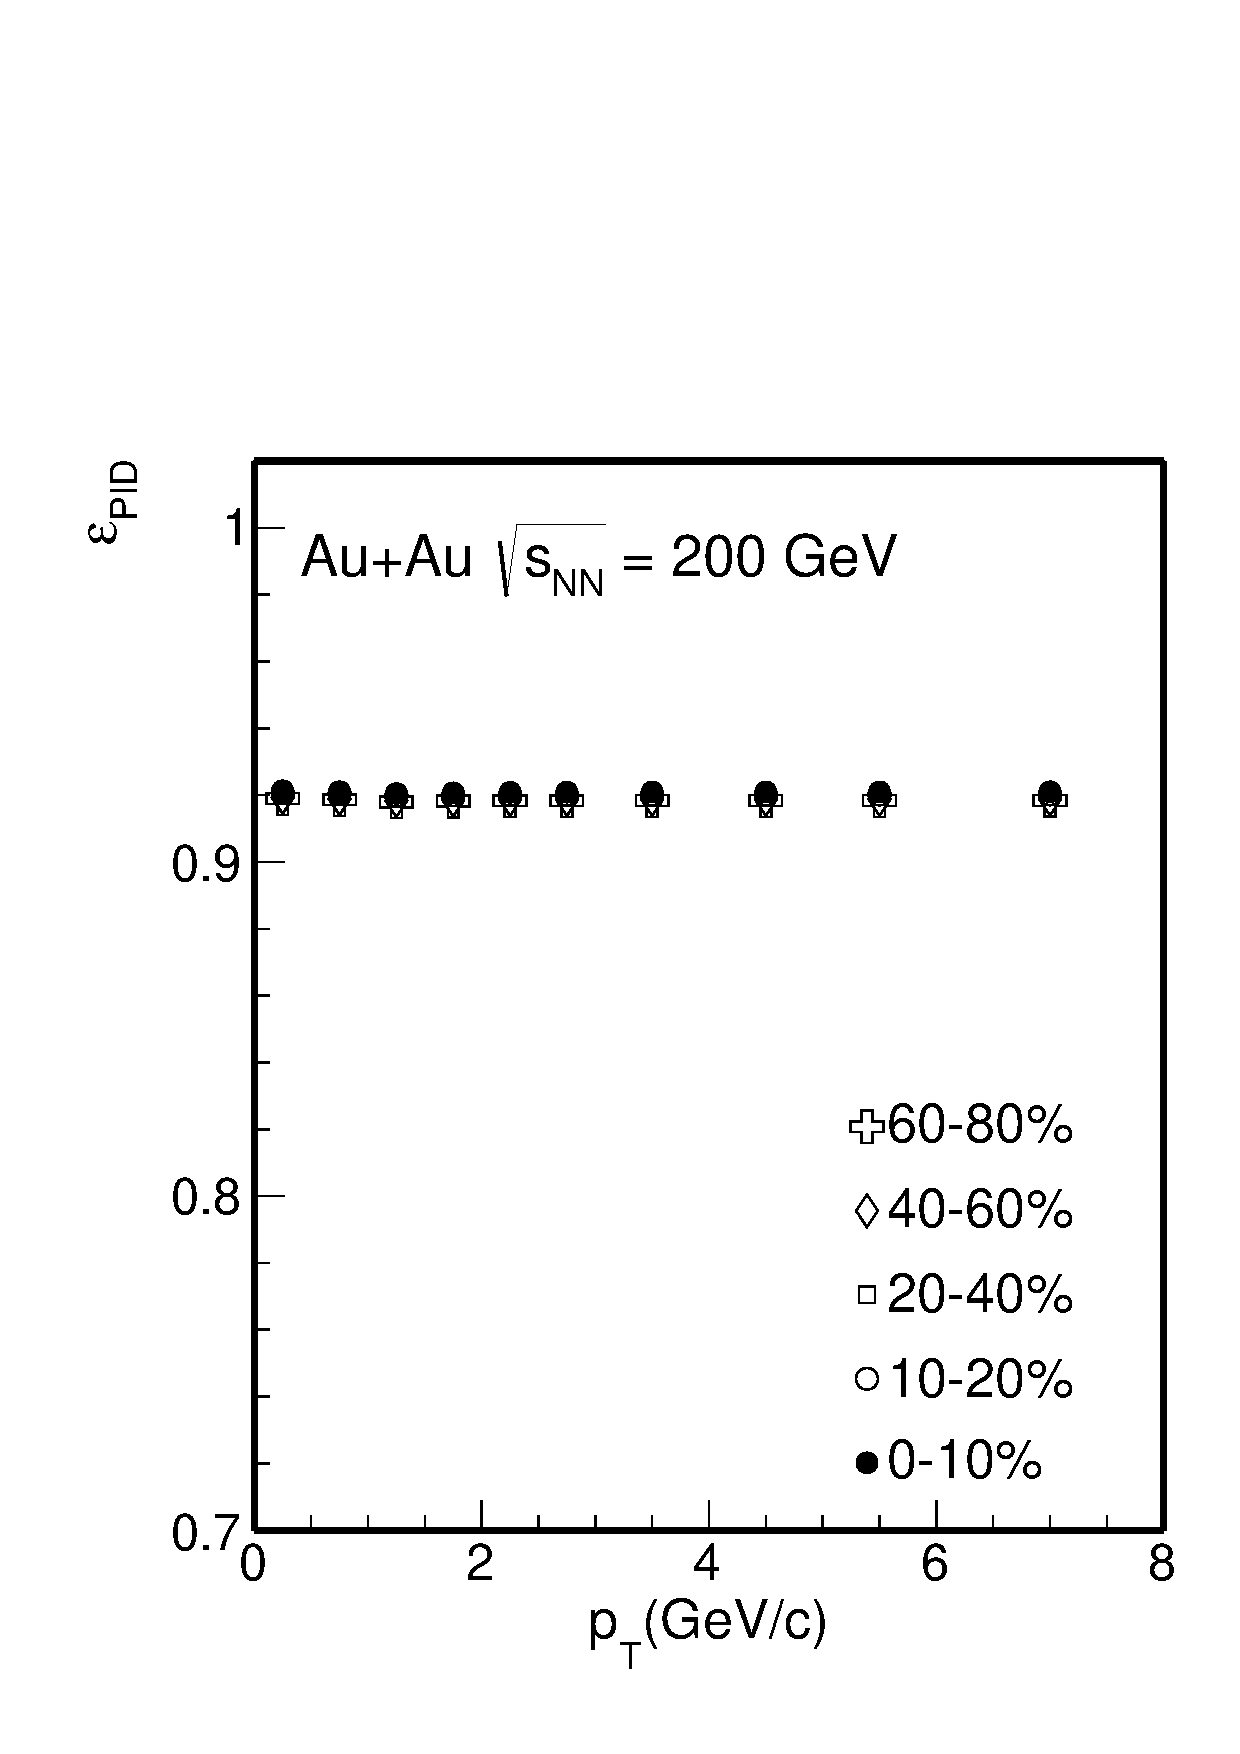
\includegraphics[width=0.4\textwidth]{fig/Datad0Eff_pid.pdf}
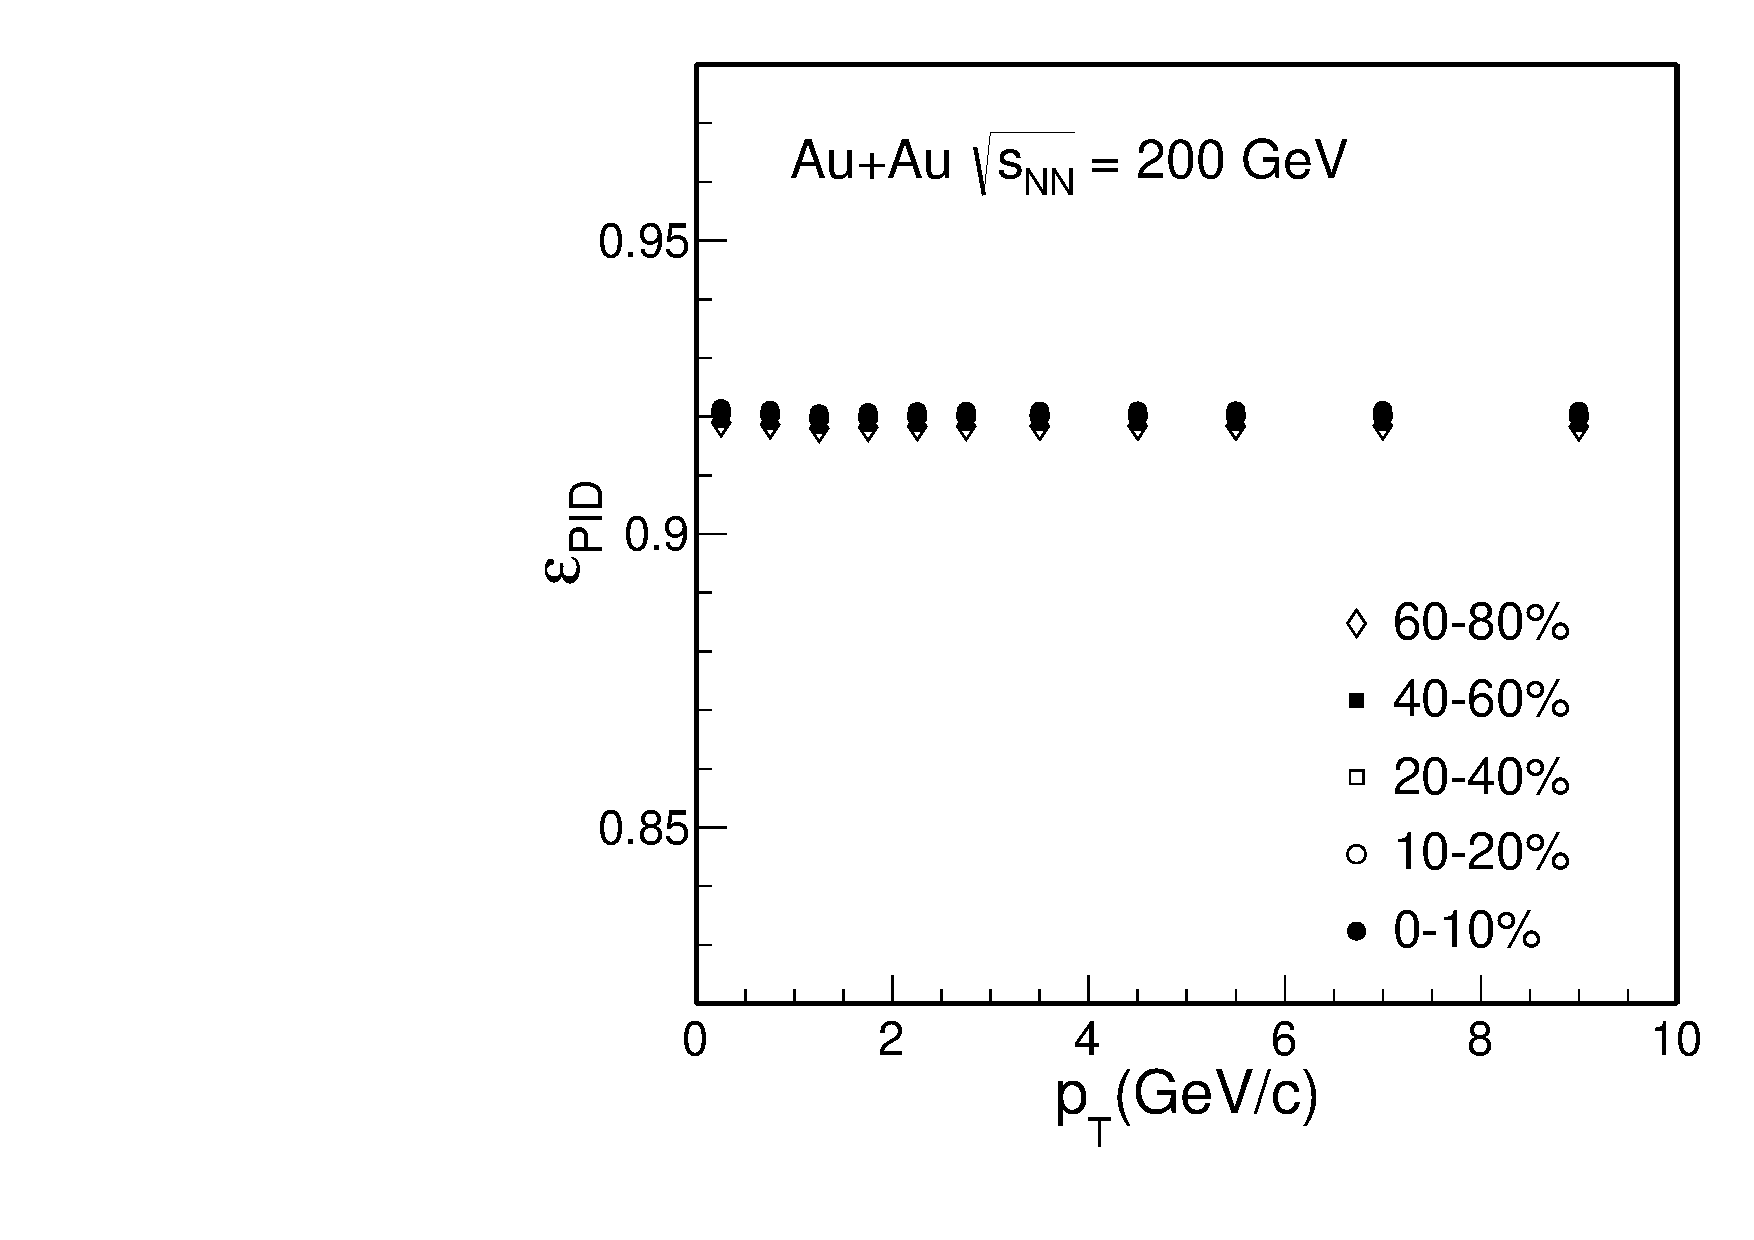
\includegraphics[width=0.43\textwidth]{fig/Datad0Eff_pid_10.pdf}
\caption{Particle identification efficiency ($\varepsilon_{\rm PID}$) of $D^0$ mesons in different centrality classes\DIFdelbeginFL \DIFdelFL{in Au + Au collisions at $\sqrt{s_{_{\rm NN}}}$ = 200\,GeV}\DIFdelendFL .}
\label{fig:Datad0Eff_pid} 
\end{figure}

\begin{figure}
\centering
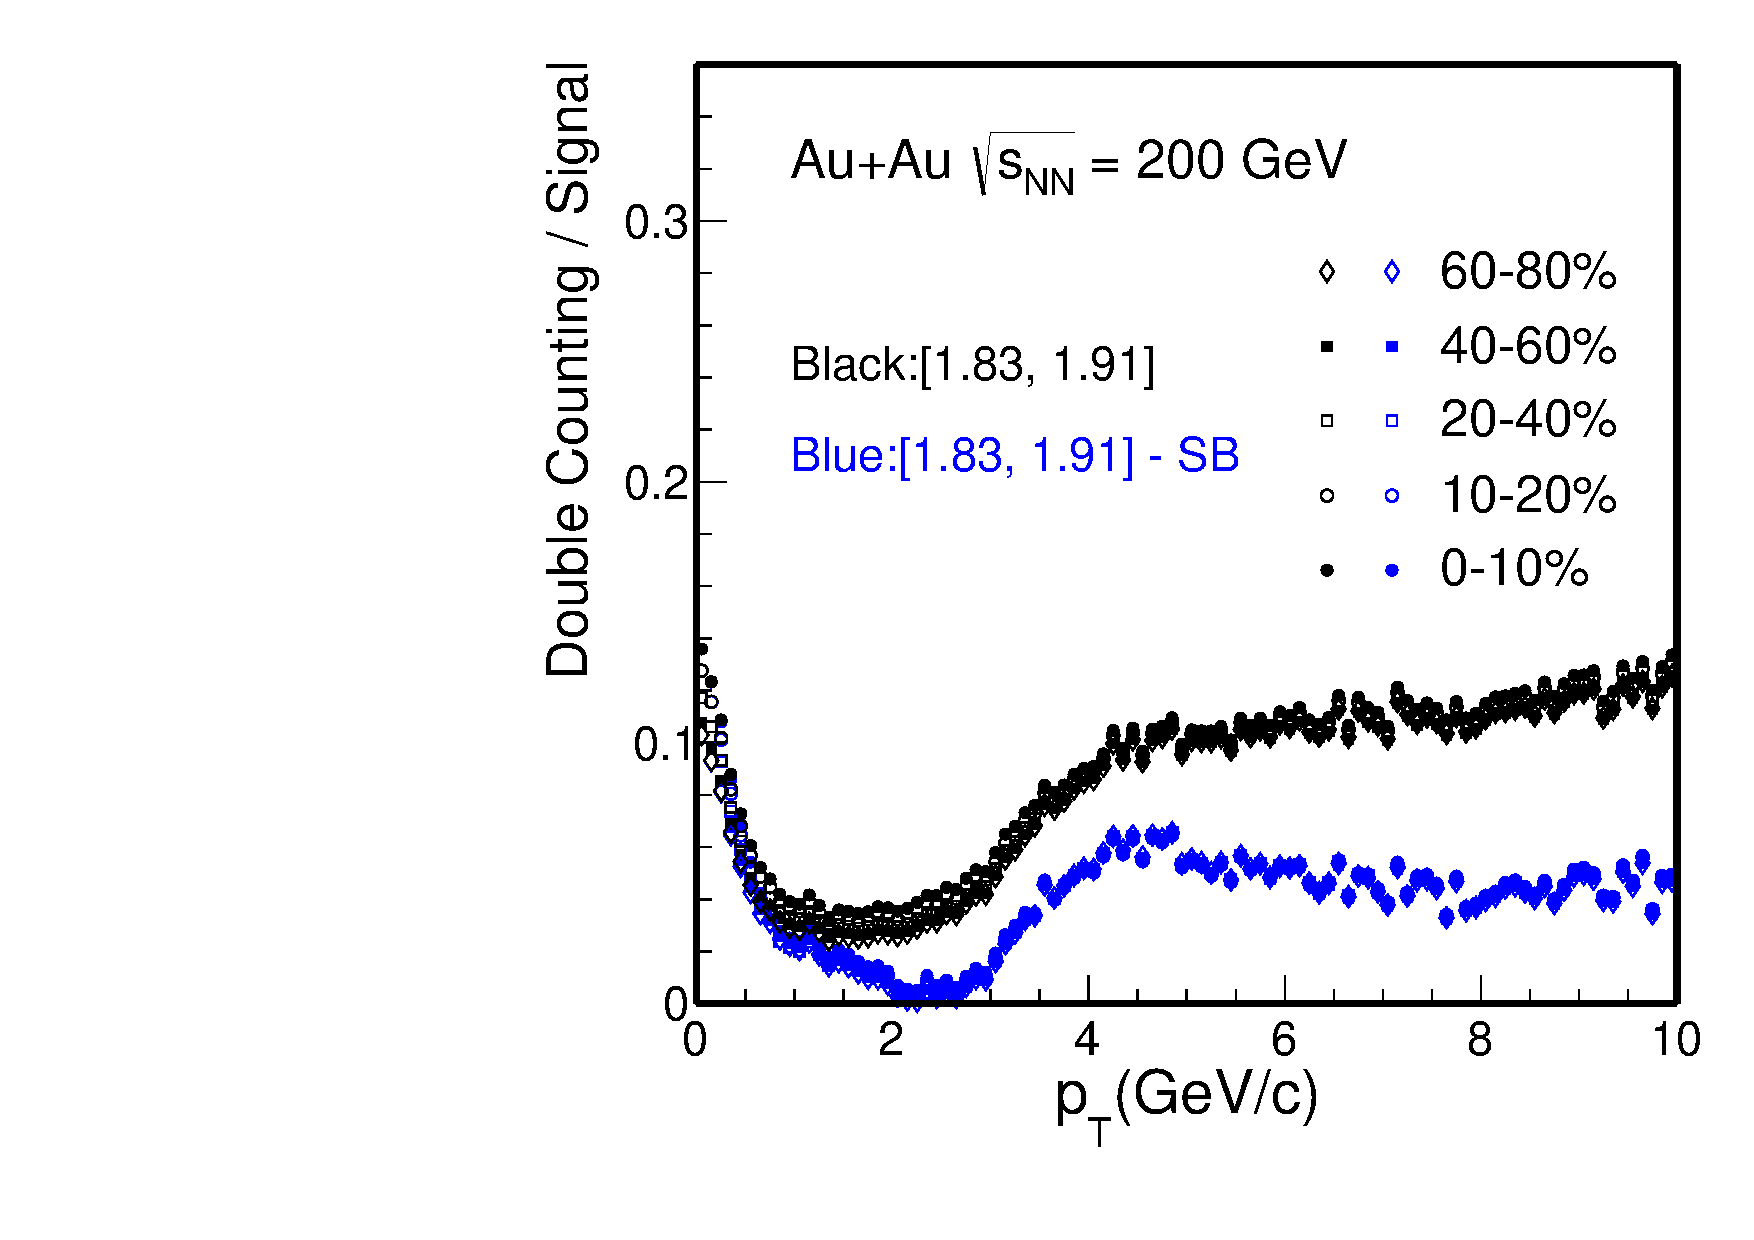
\includegraphics[width=0.43\textwidth]{fig/Double_counting.pdf}
\caption{$D^{0}$ yield double counting fraction due to doubly mis-PID in different centrality classes\DIFdelbeginFL \DIFdelFL{in Au + Au collisions at $\sqrt{s_{_{\rm NN}}}$ = 200\,GeV}\DIFdelendFL . The black markers depict an estimation taking the total double counting yield in the $D^0$ mass window while the blue markers depict an estimation with an additional side-band (SB) subtraction. \DIFaddbeginFL \DIFaddFL{No centrality dependence observed.}\DIFaddendFL }
\label{fig:Datad0Eff_doublecounting} 
\end{figure}

The $D^0$ daughter particle identification (PID) cut efficiency includes contributions from the $dE/dx$ selection cut efficiency as well as the TOF matching and $1/\beta$ cut efficiency. To best estimate the selection cut efficiency, we select the pure kaon and pion samples from V0 \DIFaddbegin \DIFadd{($\phi,K_{S}^{0}$) }\DIFaddend decay following the same procedure as in~\cite{Shao:2005iu,Xu:2008th}. The $dE/dx$ cut efficiencies for pion and kaon daughter tracks are calculated respectively. The TOF $1/\beta$ cut efficiency is determined by studying the $1/\beta$ distributions for kaons and pions in the clean separation region, namely \DIFdelbegin \DIFdel{$p_{\rm T}<$ 1.5\,GeV/$c$}\DIFdelend \DIFaddbegin \DIFadd{$p_{T}< 1.5\,\rm{GeV}/c$}\DIFaddend . There is a mild dependence for the offset and width of $\Delta 1/\beta$ distributions vs. particle momentum and our selection cuts are generally wide enough to capture nearly all tracks once they have valid $\beta$ measurements. The total PID efficiency of $D^0$ mesons is calculated by folding the individual track TPC and TOF PID efficiencies following the same hybrid PID algorithm as implemented in the data analysis. \DIFdelbegin \DIFdel{Fig.}\DIFdelend \DIFaddbegin \DIFadd{Figure}\DIFaddend ~\ref{fig:Datad0Eff_pid} shows the total PID efficiencies for $D^0$ reconstruction in various centrality bins. The total PID efficiency is generally high and \DIFdelbegin \DIFdel{there is }\DIFdelend nearly no centrality \DIFaddbegin \DIFadd{or $p_T$ }\DIFaddend dependence.

When the $D^0$ daughter kaon track is mis-identified as a pion track and the other daughter pion track is mis-identified as a kaon track, the pair invariant mass distribution will have a bump structure around the real $D^0$ signal peak, but the distribution is much broader in a wide mass region due to the mis-assigned daughter particle masses. Based on the PID  performance study described above, we estimate the single kaon and pion candidate track purities. After folding the realistic particle momentum resolution, we calculate the reconstructed $D^0$ yield from doubly mis-identified pairs (double counting) underneath the real $D^0$ signal and the double counting fraction is shown in Fig.~\ref{fig:Datad0Eff_doublecounting}. The black markers show the fraction by taking all doubly mis-identified pairs in the $D^0$ mass window while the blue markers depict \DIFdelbegin \DIFdel{that }\DIFdelend \DIFaddbegin \DIFadd{it }\DIFaddend with an additional side-band (SB) subtraction. The latter is used as a correction factor to the central values of reported $D^0$ yields while the difference between the black and blue symbols \DIFdelbegin \DIFdel{are considered as }\DIFdelend \DIFaddbegin \DIFadd{is considered }\DIFaddend the systematic uncertainty in this source. The double counting fraction is below 10\% in all \DIFdelbegin \DIFdel{$p_{\rm T}$ }\DIFdelend \DIFaddbegin \DIFadd{$p_{T}$ }\DIFaddend bins, and \DIFdelbegin \DIFdel{also }\DIFdelend there is little centrality dependence.

Figure~\ref{fig:Datad0Eff} shows the total $D^{0}$ reconstruction efficiency from different centrality classes in Au+Au collisions \DIFdelbegin \DIFdel{at $\sqrt{s_{_{\rm NN}}}$ = 200\,GeV includes each individual complement }\DIFdelend \DIFaddbegin \DIFadd{including all of the individual components }\DIFaddend discussed above.

\begin{figure}
\centering
% 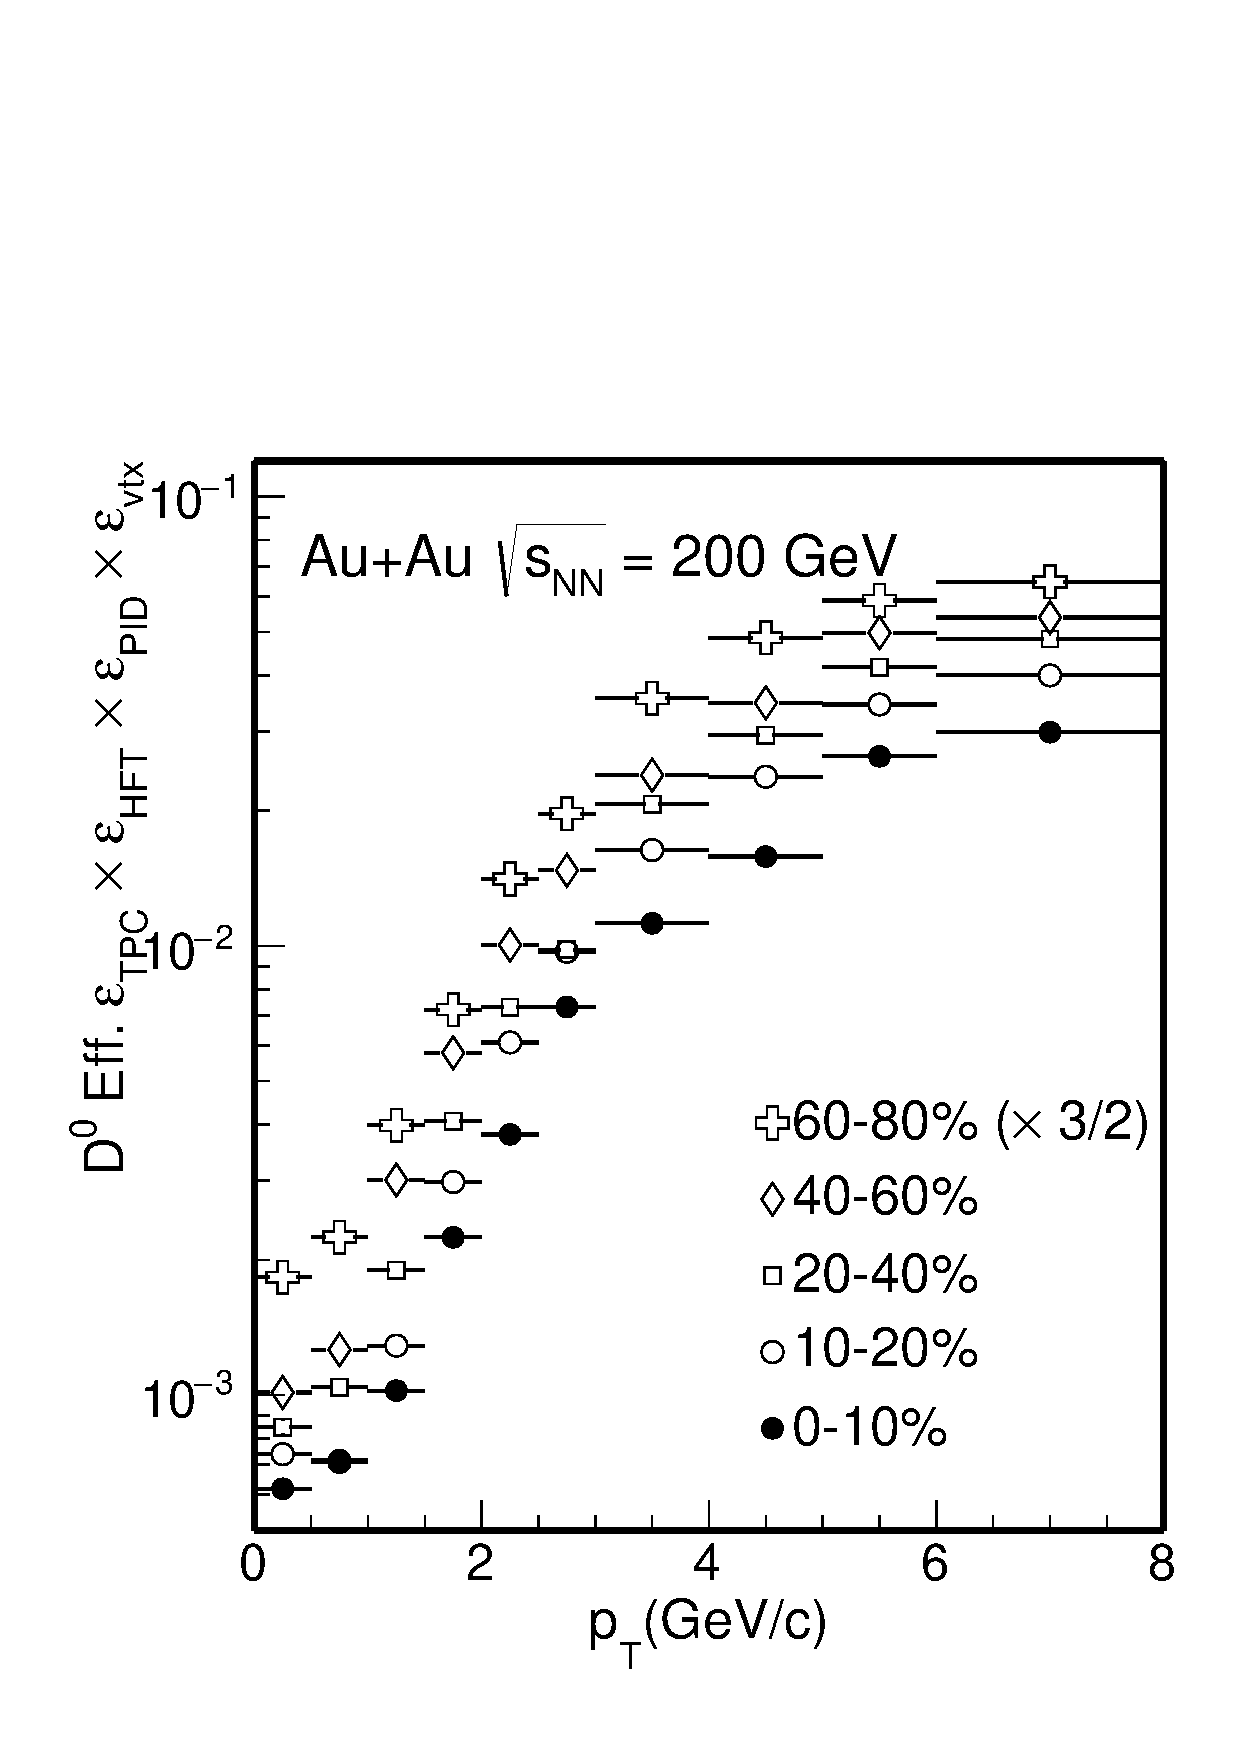
\includegraphics[width=0.4\textwidth]{fig/Datad0Eff.pdf}
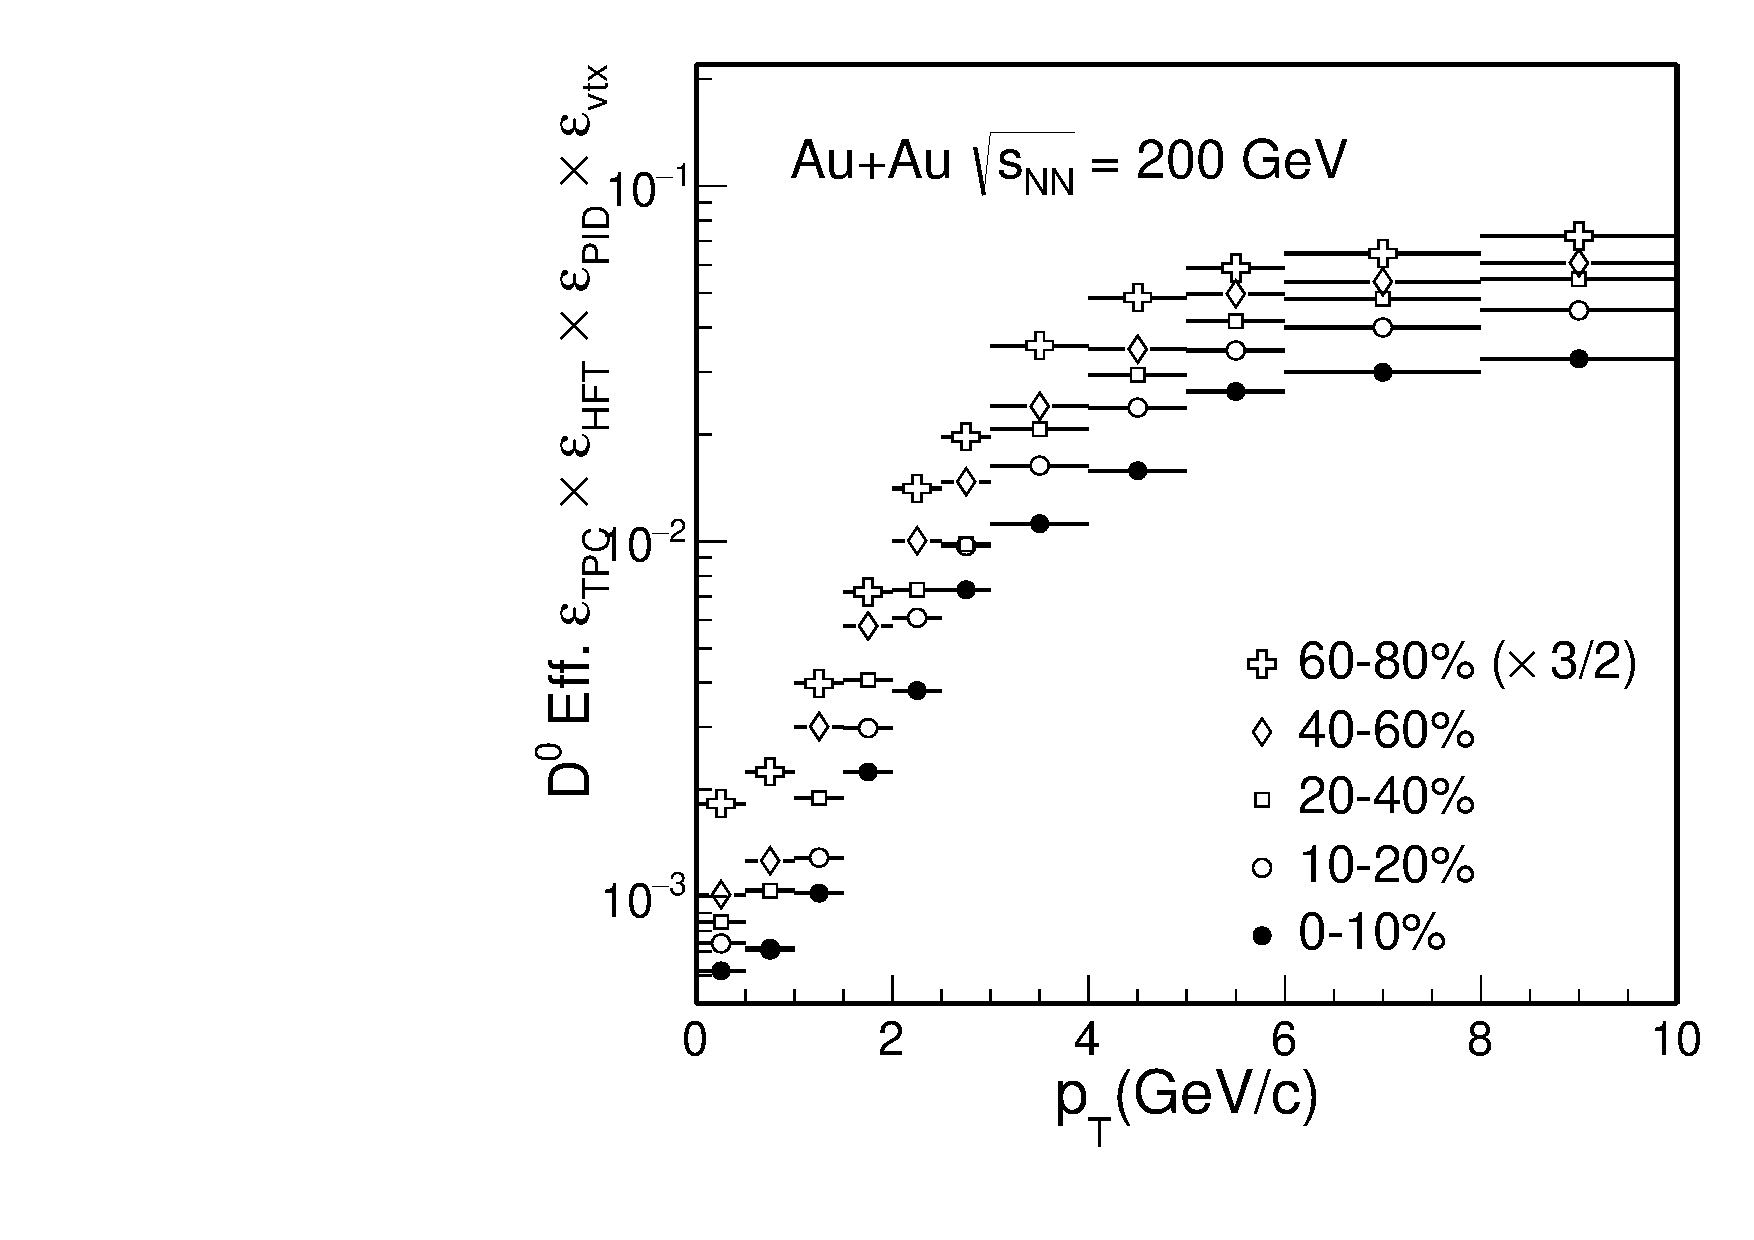
\includegraphics[width=0.43\textwidth]{fig/Datad0Eff_10.pdf}
\caption{The total $D^{0}$ reconstruction efficiency from different centrality classes\DIFdelbeginFL \DIFdelFL{in Au + Au collisions at $\sqrt{s_{_{\rm NN}}}$ = 200\,GeV}\DIFdelendFL .}
\label{fig:Datad0Eff} 
\end{figure}

\section{\DIFdelbegin %DIFDELCMD < %DIFDELCMD < \label{sec:systematic}%%%
%%%
\DIFdelend Systematic Uncertainties}
\DIFaddbegin \label{systematic}
\DIFaddend 

The systematic uncertainty on the final measured $D^0$ \DIFdelbegin \DIFdel{$p_{\rm T}$ }\DIFdelend \DIFaddbegin \DIFadd{$p_{T}$ }\DIFaddend spectra can be categorized into the uncertainty of the raw $D^0$ yield extraction and the uncertainty of efficiencies and corrections.

The uncertainty of the raw yield extraction is estimated by a) the difference in the $D^0$ yield obtained with the fit and bin counting methods\DIFdelbegin \DIFdel{and }\DIFdelend \DIFaddbegin \DIFadd{, }\DIFaddend b) varying invariant mass ranges for fit and for side bands and c) varying background estimation from mixed-event and like-sign methods. The maximum difference between these scenarios is then converted to the standard deviation and added to the systematic uncertainties. It is the smallest in the mid-\DIFdelbegin \DIFdel{$p_{\rm T}$ }\DIFdelend \DIFaddbegin \DIFadd{$p_{T}$ }\DIFaddend bins due to the best signal significance and grows at both low and high \DIFdelbegin \DIFdel{$p_{\rm T}$}\DIFdelend \DIFaddbegin \DIFadd{$p_{T}$}\DIFaddend . The double counting contribution in the $D^0$ raw yield  due to mis-PID is included as another contribution to the systematic uncertainty for the $D^0$ raw yield extraction as described in Sec.~\DIFdelbegin \DIFdel{\ref{sec:correction:PID}}\DIFdelend \DIFaddbegin \DIFadd{\ref{correction:PID}}\DIFaddend .

The uncertainty of the TPC acceptance and efficiency correction $\varepsilon_{\rm TPC}$ is estimated via the standard procedure in STAR by comparing the TPC track distributions between real data and the embedding data. It is estimated to be \DIFdelbegin \DIFdel{$\sim 3-6\%$ }\DIFdelend \DIFaddbegin \DIFadd{$\sim$3--6\% }\DIFaddend for 0-10\% collisions and \DIFdelbegin \DIFdel{$\sim 3-7\%$ }\DIFdelend \DIFaddbegin \DIFadd{$\sim$3--7\% }\DIFaddend for 60-80\% collisions, and \DIFdelbegin \DIFdel{they are largely }\DIFdelend \DIFaddbegin \DIFadd{is }\DIFaddend correlated for different centralities and \DIFdelbegin \DIFdel{$p_{\rm T}$ }\DIFdelend \DIFaddbegin \DIFadd{$p_{T}$ }\DIFaddend regions. 

The uncertainty of the PID efficiency correction is estimated by varying the PID selection cuts and \DIFdelbegin \DIFdel{convert }\DIFdelend \DIFaddbegin \DIFadd{then convolute }\DIFaddend to the final corrected $D^0$ yield. 

% The uncertainty of the PID efficiency correction is estimated by varying the PID selection cuts and compare the difference in the final corrected $D^0$ yield. In addition, for the TOF PID, we also consider the finite TOF acceptance and matching efficiency uncertainty.

% {\color{red}{Guannan: please confirm the numbers below}}
To estimate the uncertainty of the HFT tracking and topological cut efficiency correction $\varepsilon_{\rm HFT}$, we employ the following procedures: a) We vary the topological variable cuts so the $D^0$ $\varepsilon_{\rm HFT}$ is changed to 50\% and 150\% of the nominal (default) efficiency and compare the efficiency corrected final $D^0$ yields. The maximum difference between the two scenarios is then added to the systematic uncertainties. b) We also vary the daughter \DIFdelbegin \DIFdel{$p_{\rm T}$ }\DIFdelend \DIFaddbegin \DIFadd{$p_{T}$ }\DIFaddend low threshold cut between 0.3 to 0.6 GeV/$c$ and the maximum difference in the final corrected $D^0$ yield is also included in the systematic uncertainties. c) We add the systematic uncertainty due to limitation of the data-driven simulation approach, $\sim$5\%\DIFaddbegin \DIFadd{, }\DIFaddend and the impact of the secondary particles\DIFaddbegin \DIFadd{, }\DIFaddend $\sim$2\%\DIFaddbegin \DIFadd{, }\DIFaddend to the total $\varepsilon_{\rm HFT}$ systematic uncertainty.% for the 0-20\% central collisions.

With the corrected $D^0$ transverse momentum spectra, \DIFaddbegin \DIFadd{the }\DIFaddend nuclear modification factor $R_{\rm CP}$ is calculated as the ratio of $N_{\rm bin}$ normalized yields between central and peripheral collisions, as shown in the following formula\DIFdelbegin \DIFdel{. 
}\DIFdelend \DIFaddbegin \DIFadd{:
}\begin{equation}
%DIF >  \[
%DIF >  R_{\rm CP} = \frac{d^2N/dp_{T}dy/N_{\rm bin}|_{\rm cen}}{d^2N/dp_{T}dy/N_{\rm bin}|_{\rm peri}} 
  \DIFadd{R_{\rm CP} = \frac{d^2N/dp_{T}dy}{N_{\rm bin}} |_{\rm cen\ } \times \frac{N_{\rm bin}} }{\DIFadd{d^2N/dp_{T}dy}} \DIFadd{|_{\rm peri }.
}\end{equation}
\label{equ:equation3}
\]
\DIFaddend 

\DIFdelbegin \[
\DIFdel{R_{\rm CP} = \frac{d^2N/dp_{\rm T}dy/N_{\rm bin}|_{\rm cen}}{d^2N/dp_{\rm T}dy/N_{\rm bin}|_{\rm peri}}
}\]
%DIFAUXCMD
%DIFDELCMD < 

%DIFDELCMD < %%%
\DIFdelend The systematic uncertainties in \DIFaddbegin \DIFadd{the }\DIFaddend raw signal extraction in central and peripheral collisions are propagated as they are uncorrelated, while systematic uncertainties in many other sources are correlated or partially correlated in contributing to the measured $D^0$ yields. To best consider these correlations, we vary different variables simultaneously in central and peripheral collisions, and the difference in the final extracted $R_{\rm CP}$ value is then directly counted as systematic uncertainties in the measured $R_{\rm CP}$.

\DIFdelbegin \DIFdel{Nuclear }\DIFdelend \DIFaddbegin \DIFadd{The nuclear }\DIFaddend modification factor $R_{\rm AA}$ is calculated as the ratio of $N_{\rm bin}$ normalized yields between Au+Au and \DIFdelbegin \DIFdel{p }\DIFdelend \DIFaddbegin \DIFadd{$p$}\DIFaddend +\DIFdelbegin \DIFdel{p }\DIFdelend \DIFaddbegin \DIFadd{$p$ }\DIFaddend collisions. The baseline \DIFdelbegin \DIFdel{choose and uncertainties sources for p }\DIFdelend \DIFaddbegin \DIFadd{chosen and uncertainty sources for $p$}\DIFaddend +\DIFdelbegin \DIFdel{p }\DIFdelend \DIFaddbegin \DIFadd{$p$ }\DIFaddend collisions are the same as the publication~\DIFdelbegin \DIFdel{\mbox{%DIFAUXCMD
\cite{Star_D_RAA_corr}}%DIFAUXCMD
}\DIFdelend \DIFaddbegin \DIFadd{\mbox{%DIFAUXCMD
\cite{Star_D_RAA}}%DIFAUXCMD
}\DIFaddend . The uncertainties from the \DIFdelbegin \DIFdel{p }\DIFdelend \DIFaddbegin \DIFadd{$p$}\DIFaddend +\DIFdelbegin \DIFdel{p }\DIFdelend \DIFaddbegin \DIFadd{$p$ }\DIFaddend reference dominates this systematic uncertainty, which include the 1$\sigma$ uncertainty from the Levy fit and the difference between Levy and power-law function fits for extrapolation to low and high $p_T$, expressed as 1 standard deviation.

With the corrected $D^0$ and $\overline{D}^{0}$ transverse momentum spectra, \DIFaddbegin \DIFadd{the }\DIFaddend $\overline{D}^{0}/D^0$ ratio is calculated as a function of the transverse momentum. The systematic uncertainties in \DIFaddbegin \DIFadd{the }\DIFaddend raw signal extraction for $\overline{D}^{0}$ and $D^0$ are propagated as they are uncorrelated, while systematic uncertainties in many other sources are correlated or partially correlated in contributing to the measured $\overline{D}^{0}/D^0$ ratio. As in the $R_{\rm CP}$ systematic uncertainty estimation, we vary different variables simultaneously for $D^0$ and $\overline{D}^{0}$, and the difference in the final extracted $\overline{D}^{0}/D^0$ value is then directly counted as systematic uncertainties in the measured $\overline{D}^{0}/D^0$.

\begin{table*}
\DIFdelbeginFL %DIFDELCMD < \centering{
%DIFDELCMD < \caption{Summary of systematic uncertainties, in percentage, on the $D^0$ invariant yield in 0-10\% and 60-80\% collisions and $R_{\rm CP}$(0-10\%/60-80\%).}
%DIFDELCMD < \begin{tabular}{c|cc|c|c} \hline \hline
%DIFDELCMD < Source & \multicolumn{3}{c|}{Systematic Uncertainty} & Correlation in $p_{\rm T}$\\ \cline{2-4}
%DIFDELCMD <        & \hspace{1cm}0--10\%\hspace{1cm} & \hspace{1cm}60--80\%\hspace{1cm} & \hspace{1cm}$R_{\rm CP}$(0--10\%/60--80\%)\hspace{1cm} &  \\ \hline \hline
%DIFDELCMD < Signal extra. & 1-6  & 1-12  & 2-13\ & uncorr. \\ \hline
%DIFDELCMD < Double mis-PID & 1-7  & 1-7  & negligible & uncorr. \\ \hline \hline
%DIFDELCMD < % $\varepsilon_{\rm TPC}$ & 3-6 & 3-7 & 3-7 & largely corr. \\ \hline
%DIFDELCMD < $\varepsilon_{\rm TPC}$ & 5-7 & 5-8 & 3-7 & largely corr. \\ \hline
%DIFDELCMD < $\varepsilon_{\rm HFT}$ & 3-15 & 3-20 & 3-20 & largely corr. \\ \hline
%DIFDELCMD < $\varepsilon_{\rm PID}$ & 3 & 3 & negligible & largely corr. \\ \hline
%DIFDELCMD < $\varepsilon_{\rm vtx}$ & 5 & 9-18 & 10-18 & largely corr. \\ \hline
%DIFDELCMD < BR. & \multicolumn{2}{c|}{0.5} & 0 & global \\ \hline \hline
%DIFDELCMD < $N_{\rm bin}$ & 2.8 & 42 & 42 & global \\ \hline \hline
%DIFDELCMD < \end{tabular}
%DIFDELCMD < }
%DIFDELCMD < %%%
\DIFdelendFL \DIFaddbeginFL \centering{
\caption{Summary of systematic uncertainties, in percentage, on the $D^0$ invariant yield in 0-10\% and 60-80\% collisions and $R_{\rm CP}$(0-10\%/60-80\%).}
\begin{tabular}{c|cc|c|c} \hline \hline
  Source & \multicolumn{3}{c|}{Systematic uncertainty [\%]} & Correlation in $p_{T}$\\ \cline{2-4}
       & \hspace{1cm}0--10\%\hspace{1cm} & \hspace{1cm}60--80\%\hspace{1cm} & \hspace{1cm}$R_{\rm CP}$(0--10\%/60--80\%)\hspace{1cm} &  \\ \hline \hline
Signal extra. & 1-6  & 1-12  & 2-13\ & uncorr. \\ \hline
Double mis-PID & 1-7  & 1-7  & negligible & uncorr. \\ \hline \hline
% $\varepsilon_{\rm TPC}$ & 3-6 & 3-7 & 3-7 & largely corr. \\ \hline
$\varepsilon_{\rm TPC}$ & 5-7 & 5-8 & 3-7 & largely corr. \\ \hline
$\varepsilon_{\rm HFT}$ & 3-15 & 3-20 & 3-20 & largely corr. \\ \hline
$\varepsilon_{\rm PID}$ & 3 & 3 & negligible & largely corr. \\ \hline
$\varepsilon_{\rm vtx}$ & 5 & 9-18 & 10-18 & largely corr. \\ \hline
BR. & \multicolumn{2}{c|}{0.5} & 0 & global \\ \hline \hline
$N_{\rm bin}$ & 2.8 & 42 & 42 & global \\ \hline \hline
\end{tabular}
}
\DIFaddendFL \label{table:syserror}
\end{table*}


Table~\ref{table:syserror} summarizes the systematic \DIFdelbegin \DIFdel{uncertainty sources }\DIFdelend \DIFaddbegin \DIFadd{uncertainties }\DIFaddend and their contributions, in percentage, on the $D^0$ invariant yield in 0-10\% and 60-80\% collisions and $R_{\rm CP}$(0-10\%/60-80\%). In the last column we also comment on the correlation in \DIFdelbegin \DIFdel{$p_{\rm T}$ }\DIFdelend \DIFaddbegin \DIFadd{$p_{T}$ }\DIFaddend for each individual source. Later when reporting \DIFdelbegin \DIFdel{$p_{\rm T}$ }\DIFdelend \DIFaddbegin \DIFadd{$p_{T}$ }\DIFaddend integrated yields or $R_{\rm CP}$, systematic uncertainties are calculated under the following considerations: a) for \DIFdelbegin \DIFdel{$p_{\rm T}$ }\DIFdelend \DIFaddbegin \DIFadd{$p_{T}$ }\DIFaddend uncorrelated sources, we take the quadratic sum of various \DIFdelbegin \DIFdel{$p_{\rm T}$ }\DIFdelend \DIFaddbegin \DIFadd{$p_{T}$ }\DIFaddend bins; b) for sources that are largely correlated in \DIFdelbegin \DIFdel{$p_{\rm T}$}\DIFdelend \DIFaddbegin \DIFadd{$p_{T}$}\DIFaddend , we take the arithmetic sum as \DIFdelbegin \DIFdel{an }\DIFdelend \DIFaddbegin \DIFadd{a }\DIFaddend conservative estimate.

%The systematic uncertainties are studied for the spectra and $R_{\rm CP}$ analysis. Several sources are contributed to the uncertainties. Such as the TPC tracking, the raw yield extraction, the daughter $p_T$ cut scan, the topological cuts scan, the double counting and the vertex resolution contribution and so on. %The TPC uncertainties are studied by comparison of the tracking performance from real data and the MC simulation. A few different methods are used to extract the raw $D^0$ signal counts, for example using the like-sign method or mixed-event technique to subtract the combinatorial background, or using the binning counting method instead of directly fitting method to extract the yield. Several different daughter $p_T$ cuts are applied on the $D^0$ reconstruction and corrected for the efficiency. We also varied the topological variables for the reconstruction with a quite different reconstruction efficiency. The mis-identification from the daughter particles are studied. The vertex resolution is also discussed in the previous section.

% Chapter four
\DIFdelbegin \DIFdel{\
}\section{%DIFDELCMD < %DIFDELCMD < \label{result}%%%
%%%
\DIFdel{Results and Discussion}}
%DIFAUXCMD
\addtocounter{section}{-1}%DIFAUXCMD
\DIFdelend 

\DIFaddbegin \section{\DIFadd{Results and Discussion}}
\label{result}

\DIFaddend \subsection{\DIFdelbegin %DIFDELCMD < %DIFDELCMD < \label{result:pt}%%%
%%%
\DIFdel{$p_{\rm T}$ }\DIFdelend \DIFaddbegin \DIFadd{$p_{T}$ }\DIFaddend Spectra and Integrated Yields}
\DIFaddbegin \label{result:pt}

\DIFaddend Figure~\ref{fig:D0_spectra} shows the efficiency-corrected $D^0$ invariant yield at mid-rapidity ($|y|<1$) vs. \DIFdelbegin \DIFdel{$p_{\rm T}$ }\DIFdelend \DIFaddbegin \DIFadd{$p_{T}$ }\DIFaddend in 0--10\%, 10--20\%, 20--40\%, 40--60\% \DIFdelbegin \DIFdel{, }\DIFdelend \DIFaddbegin \DIFadd{and }\DIFaddend 60--80\% \DIFdelbegin \DIFdel{and 0--80\% }\DIFdelend Au+Au collisions\DIFdelbegin \DIFdel{at $\sqrt{s_{_{\rm NN}}}$ = 200\,GeV}\DIFdelend . $D^0$ spectra in some centrality bins are arbitrarily scaled with factors indicated on the plot for clarity. Dashed and solid lines depict fits to the spectra with the Levy function\DIFaddbegin \DIFadd{:
}\DIFaddend 

\DIFdelbegin %DIFDELCMD < \begin{widetext}
%DIFDELCMD < %%%
\[
\DIFdel{\frac{d^2N}{2\pi p_{\rm T}dp_{\rm T}dy} = \frac{1}{2\pi}\frac{dN}{dy}\frac{(n-1)(n-2)}{nT(nT+m_0(n-2))}\bigg(1+\frac{\sqrt{p_{\rm T}^2+m_0^2}-m_0}{nT}\bigg)^{-n}
}\]
%DIFAUXCMD
%DIFDELCMD < \end{widetext}
%DIFDELCMD < 

%DIFDELCMD < %%%
\DIFdelend \DIFaddbegin \begin{equation}
  \DIFadd{\begin{aligned}
% \begin{widetext}
% \[
    \frac{d^2N}{2\pi p_{T}dp_{T}dy} = 
   & \frac{1}{2\pi}\frac{dN}{dy}\frac{(n-1)(n-2)}{nT(nT+m_0(n-2))} \\
  & \times \bigg(1+\frac{\sqrt{p_{T}^2+m_0^2}-m_0}{nT}\bigg)^{-n},
% \end{aligned}
%DIF >  \end{widetext}
  }\end{equation}
\label{equ:equation4}
\]
\DIFaddend where $m_0$ is the $D^0$ mass \DIFaddbegin \DIFadd{(1.864 GeV/$c^2$) }\DIFaddend and $\frac{dN}{dy}$, $T$ and $n$ are free parameters. The Levy function fit describes the $D^0$ spectra nicely in all centrality bins up to 8\,GeV/$c$.


\begin{figure}
\centering
\DIFdelbeginFL %DIFDELCMD < 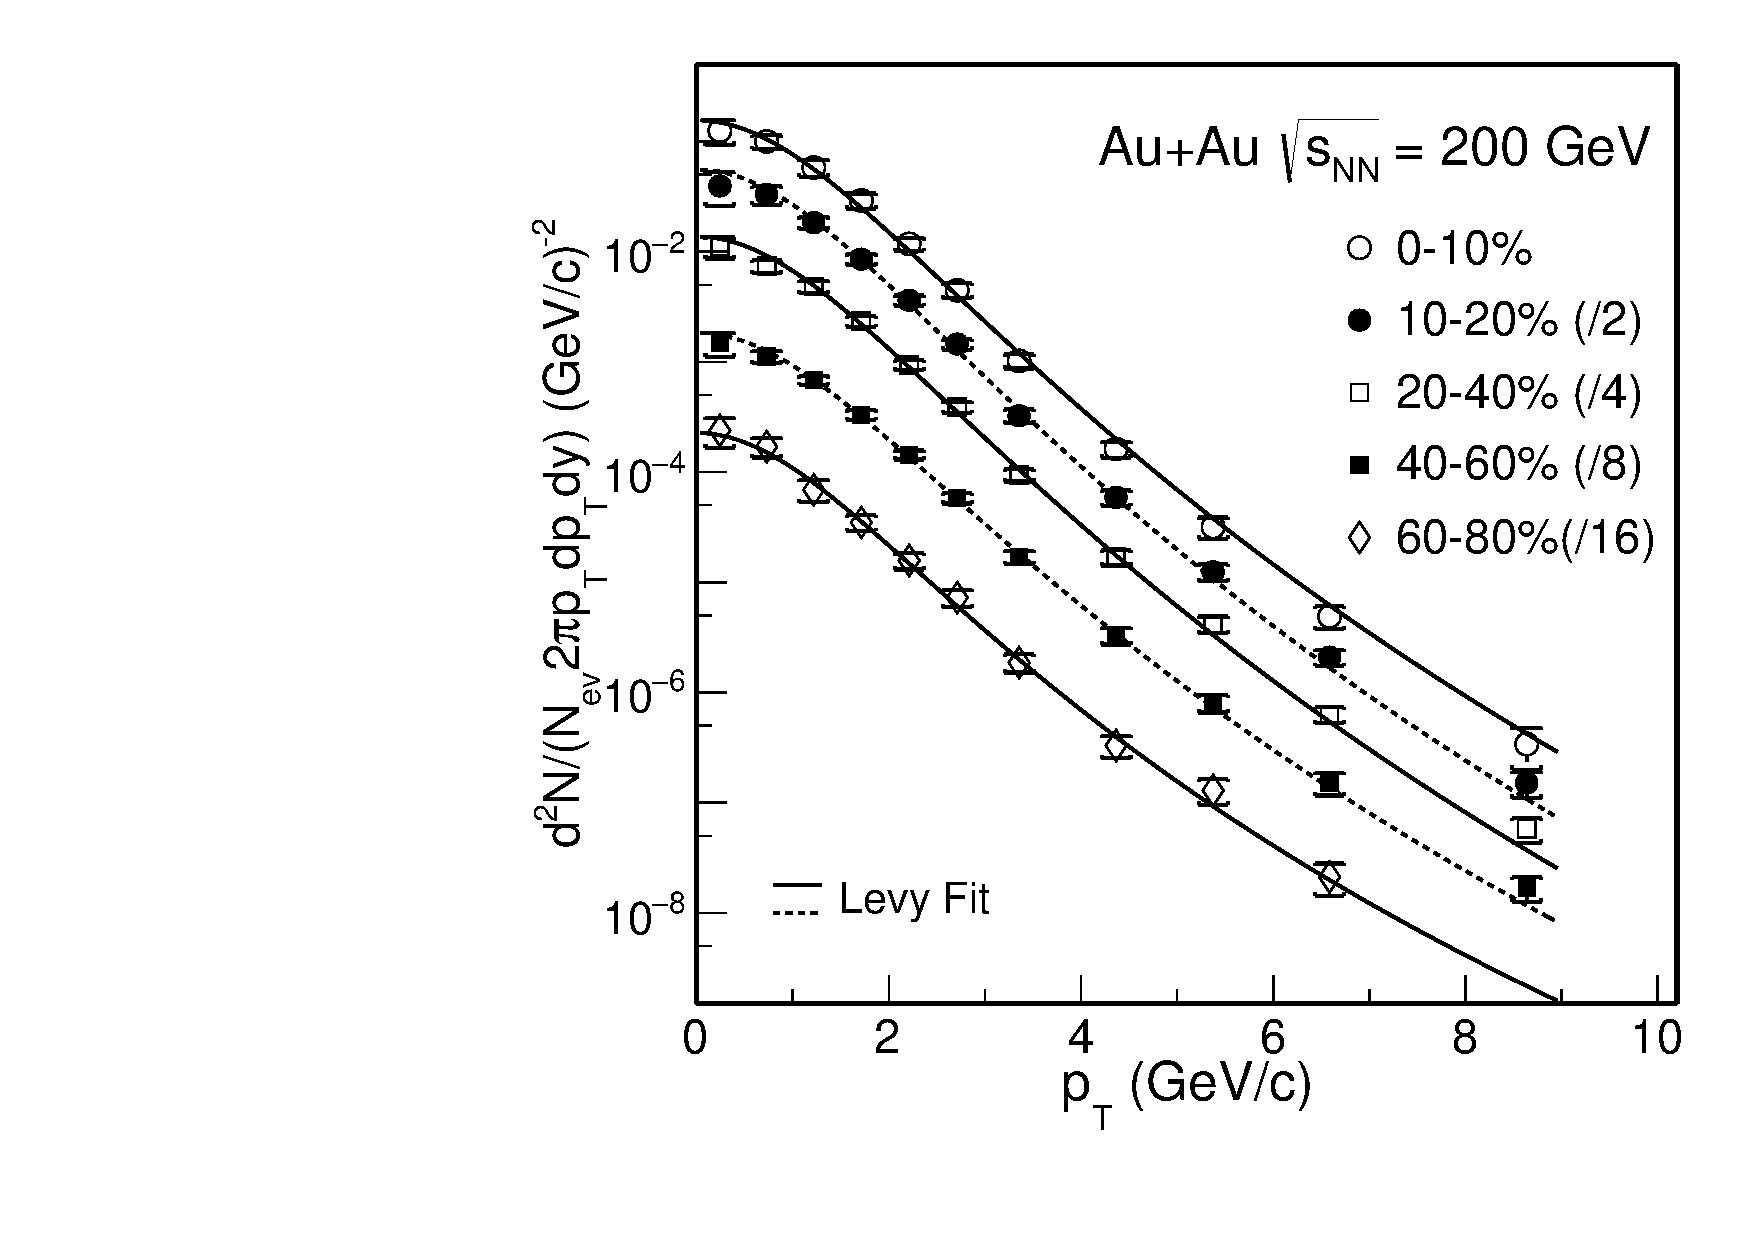
\includegraphics[width=0.43\textwidth]{fig/D0_spectra.pdf}
%DIFDELCMD < %%%
\DIFdelendFL \DIFaddbeginFL \includegraphics[width=0.43\textwidth]{fig/D0_spectra.eps}
\DIFaddendFL \caption{$D^{0}$ invariant yield at mid-rapidity ($|y|<1$) vs. transverse momentum for different centrality classes\DIFdelbeginFL \DIFdelFL{in Au + Au collisions at $\sqrt{s_{_{\rm NN}}}$ = 200\,GeV}\DIFdelendFL . Error bars (not visible for many data points) indicate statistical uncertainties and brackets depict \DIFdelbeginFL \DIFdelFL{systematical }\DIFdelendFL \DIFaddbeginFL \DIFaddFL{systematic }\DIFaddendFL uncertainties. Global systematic uncertainties in $B.R.$ are not plotted. Solid and dashed lines depict Levy function fits.}
\label{fig:D0_spectra} 
\end{figure}


We compare our new measurements with previous measurements using the STAR TPC only. The previous measurements are recently corrected after fixing errors in the TOF PID efficiency calculation~\DIFdelbegin \DIFdel{\mbox{%DIFAUXCMD
\cite{Star_D_RAA,Star_D_RAA_corr}}%DIFAUXCMD
. Fig.}\DIFdelend \DIFaddbegin \DIFadd{\mbox{%DIFAUXCMD
\cite{Star_D_RAA}}%DIFAUXCMD
. Figure}\DIFaddend ~\ref{fig:D0_compareSpectra_run10} shows the \DIFdelbegin \DIFdel{$p_{\rm T}$ }\DIFdelend \DIFaddbegin \DIFadd{$p_{T}$ }\DIFaddend spectra comparison in 0--10\%, 10-40\% and 40--80\% centrality bins in panel (a) and the ratios to the \DIFdelbegin \DIFdel{levy fit functions are shown in panel }\DIFdelend \DIFaddbegin \DIFadd{Levy fit functions in panels }\DIFaddend (b), (c), and (d). The new measurement with the HFT detector shows a nice agreement with the measurement without the HFT, but with significantly improved precision.

\begin{figure}
\centering
\DIFdelbeginFL %DIFDELCMD < \includegraphics[width=0.43\textwidth]{fig/D0_compareSpectra_run10.eps}
%DIFDELCMD < %%%
\DIFdelendFL \DIFaddbeginFL \includegraphics[width=0.44\textwidth]{fig/D0_compareSpectra_run10.eps}
  \DIFaddendFL \caption{\DIFaddbeginFL \DIFaddFL{(a) }\DIFaddendFL Measured $D^{0}$ spectra from this analysis compared with the previous 2010/11 measurements for different centrality classes\DIFdelbeginFL \DIFdelFL{in Au + Au collisions at $\sqrt{s_{_{\rm NN}}}$ = 200\,GeV}\DIFdelendFL . \DIFaddbeginFL \DIFaddFL{Dashed lines depict Levy function fits to 2014 data. (b) - (d), Ratio of measured spectra to the fitted Levy function.}\DIFaddendFL }
\label{fig:D0_compareSpectra_run10} 
\end{figure}


The measured $D^0$ spectra cover a wide \DIFdelbegin \DIFdel{$p_{\rm T}$ }\DIFdelend \DIFaddbegin \DIFadd{$p_{T}$ }\DIFaddend region which allows us to extract the \DIFdelbegin \DIFdel{$p_{\rm T}$ }\DIFdelend \DIFaddbegin \DIFadd{$p_{T}$ }\DIFaddend integrated total $D^0$ yield at mid-rapidity with good precision. \DIFdelbegin \DIFdel{Fig.}\DIFdelend \DIFaddbegin \DIFadd{Figure}\DIFaddend ~\ref{fig:Xsection_D0} shows the \DIFdelbegin \DIFdel{$p_{\rm T}$ }\DIFdelend \DIFaddbegin \DIFadd{$p_{T}$ }\DIFaddend integrated cross section \DIFdelbegin \DIFdel{$d\sigma/dy|_{y=0}$ }\DIFdelend \DIFaddbegin \DIFadd{$d\sigma^{NN}/dy|_{y=0}$ }\DIFaddend for $D^0$ production per nucleon-nucleon collision from different centrality bins for the full \DIFdelbegin \DIFdel{$p_{\rm T}$ }\DIFdelend \DIFaddbegin \DIFadd{$p_{T}$ }\DIFaddend range shown in the top panel and for \DIFdelbegin \DIFdel{$p_{\rm T}>$ 4\,GeV/$c$ }\DIFdelend \DIFaddbegin \DIFadd{$p_{T}> 4\,\rm{GeV}/c$ }\DIFaddend shown in the bottom panel. The result from \DIFdelbegin \DIFdel{previous $p+p$ }\DIFdelend \DIFaddbegin \DIFadd{a previous $p$+$p$ }\DIFaddend measurement is also shown in the top panel.

The total $D^0$ cross section per nucleon-nucleon collision at mid-rapidity \DIFdelbegin \DIFdel{$d\sigma/dy|_{y=0}$ }\DIFdelend \DIFaddbegin \DIFadd{$d\sigma^{NN}/dy|_{y=0}$ }\DIFaddend shows approximately a flat distribution as a function of \DIFdelbegin \DIFdel{centrality}\DIFdelend \DIFaddbegin \DIFadd{$N_{\rm part}$}\DIFaddend , even though the systematic uncertainty in the 60--80\% centrality bin is a bit large. The values in mid-central to central Au+Au collisions are smaller than that in \DIFdelbegin \DIFdel{$p+p$ collisions with $\sim$ 1.5$\sigma$ }\DIFdelend \DIFaddbegin \DIFadd{$p$+$p$ collisions with $\sim1.5\sigma$ }\DIFaddend effect considering the large uncertainties from the \DIFdelbegin \DIFdel{$p+p$ }\DIFdelend \DIFaddbegin \DIFadd{$p$+$p$ }\DIFaddend measurements. The total charm quark yield in heavy-ion collisions is expected to follow the number-of-binary-collision scaling since charm quarks are believed to be predominately created at the initial hard scattering before the formation of the QGP at RHIC energies\DIFdelbegin \DIFdel{, while }\DIFdelend \DIFaddbegin \DIFadd{. However, }\DIFaddend the cold nuclear \DIFdelbegin \DIFdel{effect }\DIFdelend \DIFaddbegin \DIFadd{matter (CNM) effect including shadowing }\DIFaddend could also play an important role. In addition, \DIFdelbegin \DIFdel{coalescence hadronization mechanism }\DIFdelend \DIFaddbegin \DIFadd{hadronization through coalescence }\DIFaddend has been suggested to potentially modify the charm quark distribution in various charm hadron states which may lead to the reduction in the observed $D^0$ yields in Au+Au collisions\DIFdelbegin \DIFdel{. }\DIFdelend \DIFaddbegin \DIFadd{~\mbox{%DIFAUXCMD
\cite{GRECO2004202} }%DIFAUXCMD
(as seen in Fig.~\ref{fig:Xsection_D0}). }\DIFaddend For instance, \DIFdelbegin \DIFdel{coalescence hadronization }\DIFdelend \DIFaddbegin \DIFadd{hadronization through coalescence }\DIFaddend can lead to an enhancement \DIFdelbegin \DIFdel{in }\DIFdelend \DIFaddbegin \DIFadd{of }\DIFaddend the charmed baryon $\Lambda_{c}^+$ yield relative to $D^0$ yield~\cite{Oh2009}, and together with the strangeness enhancement in the hot QCD medium, can also lead to an enhancement in the charmed \DIFdelbegin \DIFdel{strangeness }\DIFdelend \DIFaddbegin \DIFadd{strange }\DIFaddend meson $D_{s}^+$ yield relative to $D^0$~\cite{He2013}. Therefore, determination of the total charm quark yield in heavy-ion collisions will require measurements of other charm hadron states over a broad momentum range.

\begin{figure}
\centering
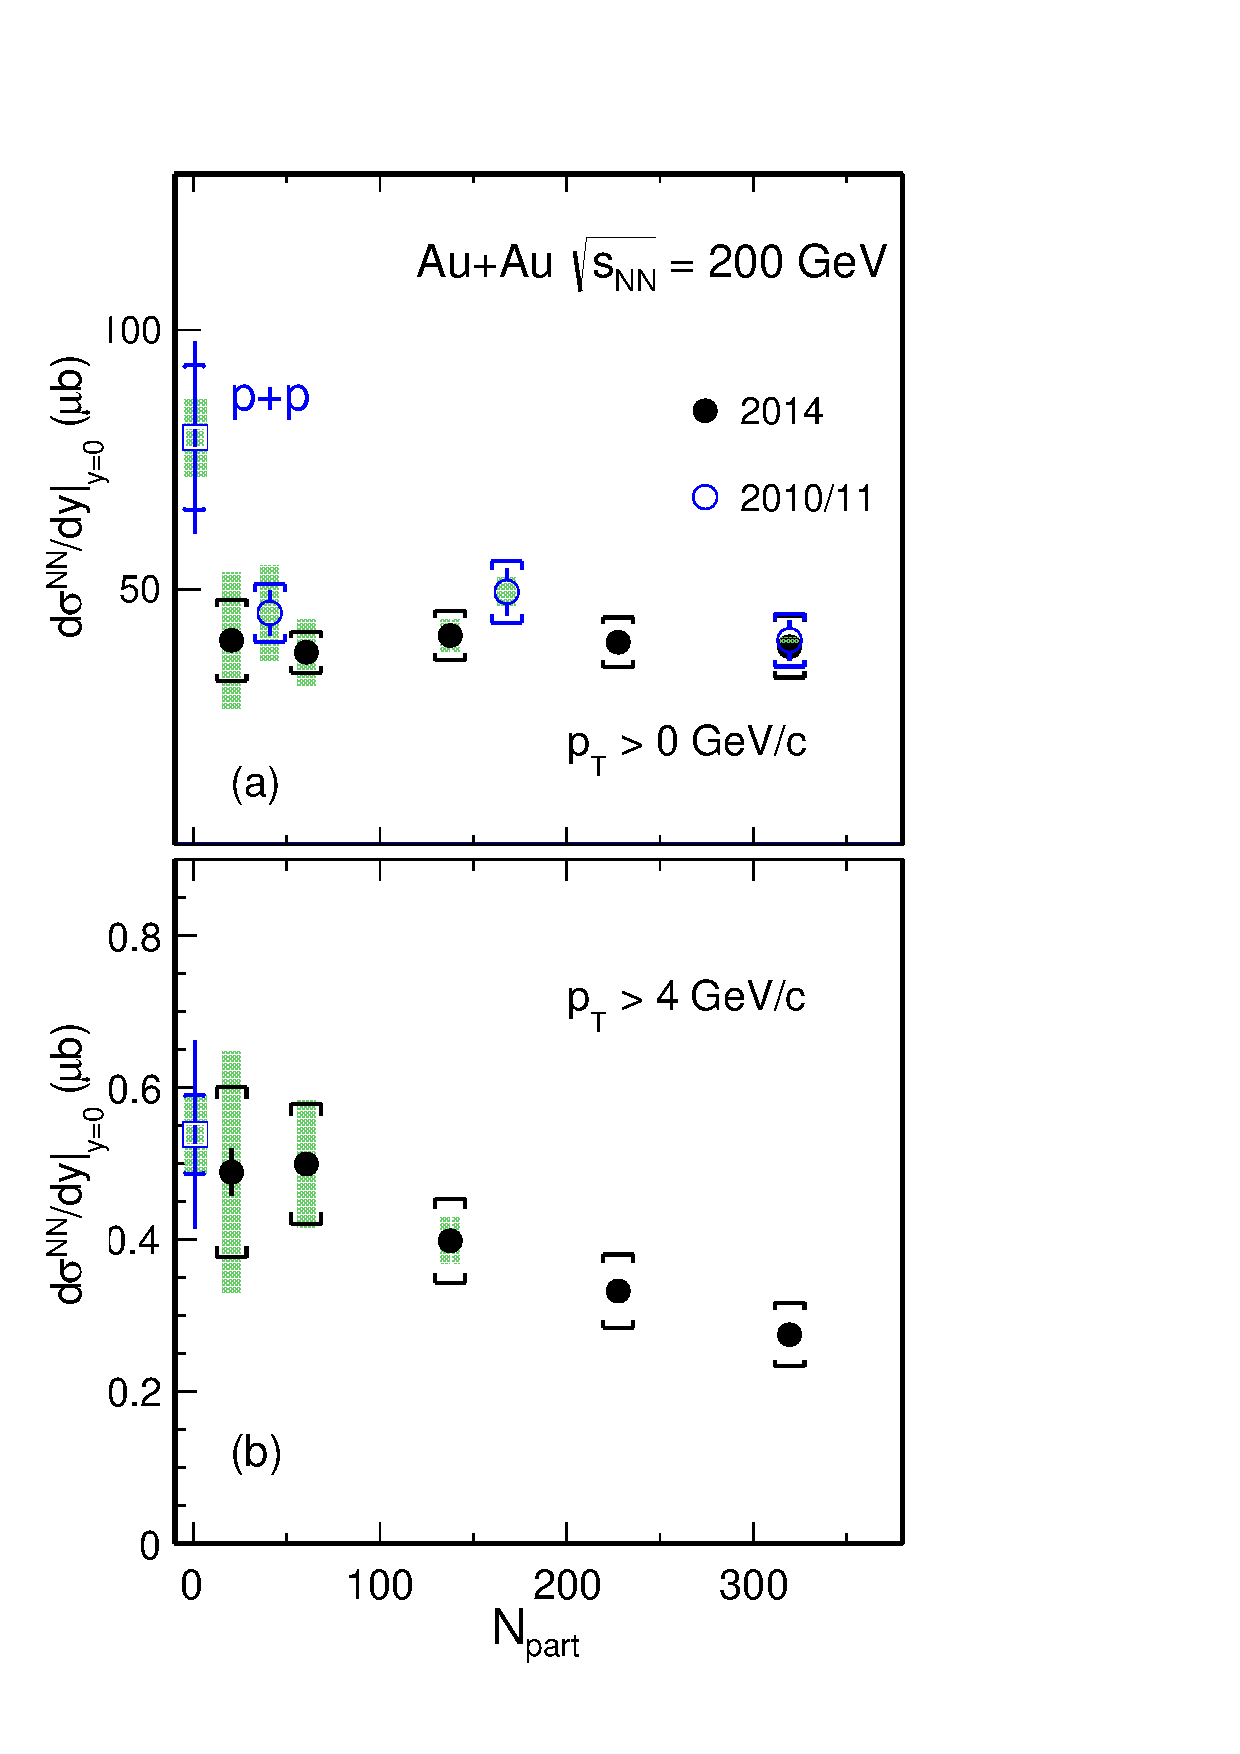
\includegraphics[width=0.43\textwidth]{fig/Xsection_D0.pdf}
  \caption{Integrated $D^{0}$ cross section at mid-rapidity per nucleon-nucleon collision at mid-rapidity for \DIFdelbeginFL \DIFdelFL{$p_{\rm T}>0$ }\DIFdelendFL \DIFaddbeginFL \DIFaddFL{$p_{T}>0$ (a) }\DIFaddendFL and \DIFdelbeginFL \DIFdelFL{$p_{\rm T}>4$}\DIFdelendFL \DIFaddbeginFL \DIFaddFL{$p_{T}>4$}\DIFaddendFL \,GeV/$c$ \DIFaddbeginFL \DIFaddFL{(b) }\DIFaddendFL as a function of centrality $N_{\rm part}$. The statistical and systematic uncertainties are shown as error bars and brackets on the data points. The green boxes on the data points depict the overall normalization uncertainties in \DIFdelbeginFL \DIFdelFL{p }\DIFdelendFL \DIFaddbeginFL \DIFaddFL{$p$}\DIFaddendFL +\DIFdelbeginFL \DIFdelFL{p }\DIFdelendFL \DIFaddbeginFL \DIFaddFL{$p$ }\DIFaddendFL and Au+Au data respectively.}
\label{fig:Xsection_D0} 
\end{figure}

\subsection{\DIFdelbegin %DIFDELCMD < %DIFDELCMD < \label{result:collectivity}%%%
%%%
\DIFdelend Collectivity}
\DIFaddbegin \label{result:collectivity}
\DIFaddend 

\subsubsection{\DIFdelbegin %DIFDELCMD < %DIFDELCMD < \label{result:collectivity:mT}%%%
%%%
\DIFdelend $m_{\rm T}$ Spectra}
\DIFaddbegin \label{result:collectivity:mT}
\DIFaddend 

\begin{figure}
\centering
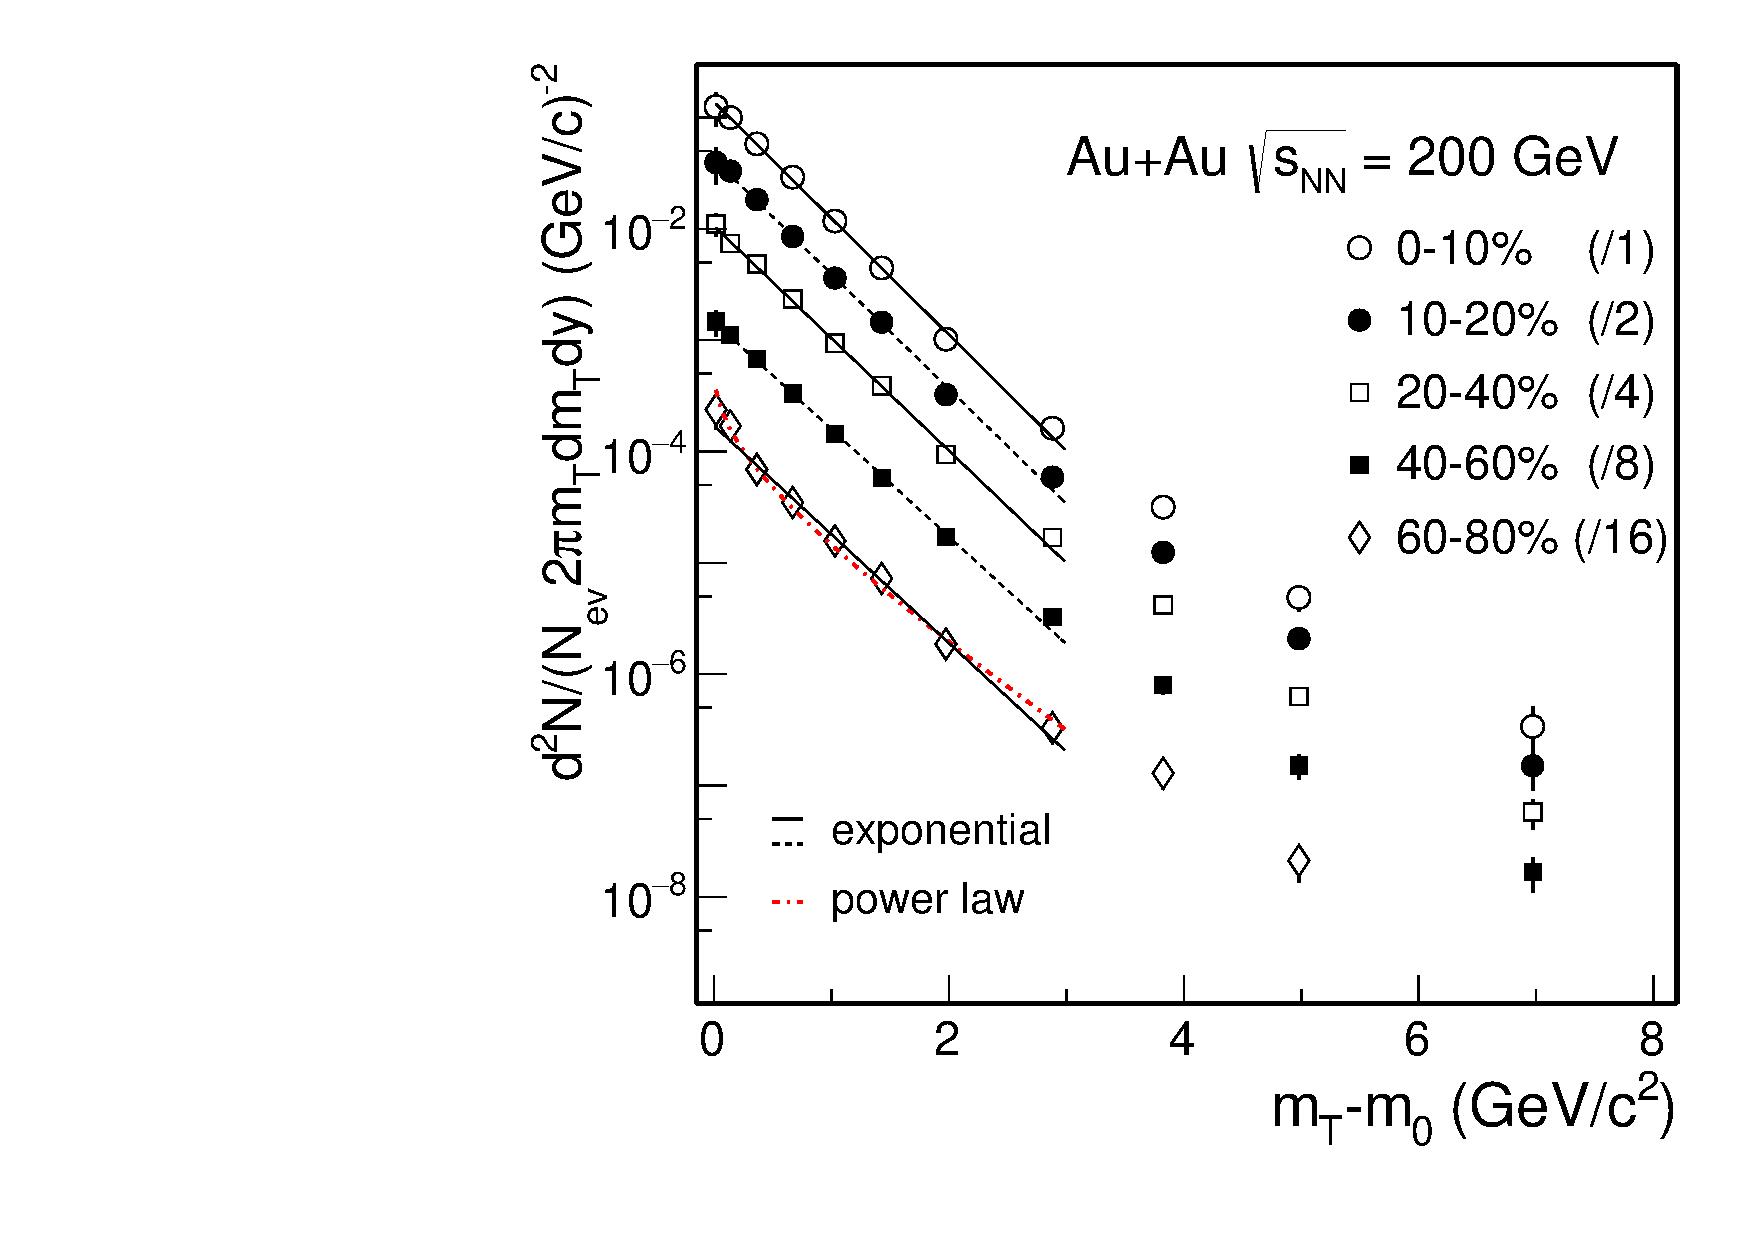
\includegraphics[width=0.43\textwidth]{fig/mTFit_D0.pdf}
\caption{$D^{0}$ invariant yield at mid-rapidity ($|y|<1$) vs. transverse kinetic energy ($m_{T}$ - $m_{0}$) for different centrality classes\DIFdelbeginFL \DIFdelFL{in Au + Au collisions at $\sqrt{s_{_{\rm NN}}}$ = 200\,GeV}\DIFdelendFL . Error bars (not visible for many data points) indicate statistical uncertainties and brackets depict \DIFdelbeginFL \DIFdelFL{systematical }\DIFdelendFL \DIFaddbeginFL \DIFaddFL{systematic }\DIFaddendFL uncertainties. Global systematic uncertainties in $B.R.$ are not plotted. Solid and dashed black lines depict exponential function fits and the dot-dashed line depict a power-law function fit to the spectrum in 60--80\% centrality bin.}
\label{fig:mTFit_D0} 
\end{figure}

Transverse mass spectra can be used to study the collectivity of produced hadrons in heavy-ion collisions. \DIFdelbegin \DIFdel{Fig.}\DIFdelend \DIFaddbegin \DIFadd{Figure}\DIFaddend ~\ref{fig:mTFit_D0} shows the $D^{0}$ invariant yield at mid-rapidity ($|y|<1$) vs. transverse kinetic energy ($m_{\rm T}$ - $m_{0}$) for different centrality classes\DIFdelbegin \DIFdel{in Au + Au collisions at $\sqrt{s_{_{\rm NN}}}$ = 200\,GeV, where $m_{\rm T} = \sqrt{p_{\rm T}^2+m_0^2}$ }\DIFdelend \DIFaddbegin \DIFadd{, where $m_{\rm T} = \sqrt{p_{T}^2+m_0^2}$ }\DIFaddend and $m_0$ is the $D^0$ meson mass. Solid and dashed black lines depict thermal model inspired exponential function fits to data in various centrality bins up to $m_{\rm T} - m_{0}$ $<3$\,GeV/$c^2$ using the fit function shown below\DIFdelbegin \[
\DIFdel{\frac{d^2N}{2\pi m_{\rm T}dm_{\rm T}dy} = \frac{dN/dy}{2\pi T_{\rm eff}(m_0+T_{\rm eff})}e^{-(m_{\rm T}-m_0)/T_{\rm eff}}
}\]
%DIFAUXCMD
\DIFdelend \DIFaddbegin \DIFadd{:
}\begin{equation}
  \DIFadd{\begin{aligned}
% \[
\frac{d^2N}{2\pi m_{\rm T}dm_{\rm T}dy} = \frac{dN/dy}{2\pi T_{\rm eff}(m_0+T_{\rm eff})}e^{-(m_{\rm T}-m_0)/T_{\rm eff}}.
% \end{aligned}
  }\end{equation}
\label{equ:equation5}
\]
\DIFaddend Such a method has been often used to analyze the particle spectra and to understand kinetic freezeout properties for the data in \DIFdelbegin \DIFdel{heavy ion }\DIFdelend \DIFaddbegin \DIFadd{heavy--ion }\DIFaddend collisions~\cite{Kaneta:1999lnf,StarWhitePaper}.


A power-law function (shown below) is also used to fit the spectrum in \DIFaddbegin \DIFadd{the }\DIFaddend 60--80\% centrality bin\DIFdelbegin \DIFdel{. 
}%DIFDELCMD < 

%DIFDELCMD < %%%
%DIF < \begin{widetext}
\[
\DIFdel{\frac{d^2N}{2\pi p_{\rm T}dp_{\rm T}dy} = \frac{dN}{dy}\frac{4(n-1)(n-2)}{2\pi (n-3)^2\langle p_{\rm T} \rangle ^2}\bigg(1+\frac{2p_{\rm T}}{\langle p_{\rm T} \rangle (n-3)}\bigg)^{-n}
}\]
%DIFAUXCMD
%DIF < \end{widetext}
%DIFDELCMD < 

%DIFDELCMD < %%%
\DIFdelend \DIFaddbegin \DIFadd{:
}\begin{equation}
  \DIFadd{\begin{aligned}
%\begin{widetext}
% \[
\frac{d^2N}{2\pi p_{T}dp_{T}dy} = \frac{dN}{dy}\frac{4(n-1)(n-2)}{2\pi (n-3)^2\langle p_{T} \rangle ^2}\bigg(1+\frac{2p_{T}}{\langle p_{T} \rangle (n-3)}\bigg)^{-n},
% \end{aligned}
%DIF > \end{widetext}
  }\end{equation}
\label{equ:equation6}
\]
\DIFaddend where $dN/dy$, \DIFdelbegin \DIFdel{$\langle p_{\rm T}\rangle$}\DIFdelend \DIFaddbegin \DIFadd{$\langle p_{T}\rangle$}\DIFaddend , and $n$ are three free parameters.

The power-law function fit shows a good description \DIFdelbegin \DIFdel{to }\DIFdelend \DIFaddbegin \DIFadd{of }\DIFaddend the 60--80\% centrality data indicating \DIFaddbegin \DIFadd{that }\DIFaddend the $D^0$ meson production in this peripheral bin is close to the expected feature of \DIFdelbegin \DIFdel{the }\DIFdelend perturbative QCD. The $D^0$ meson spectra in more central collisions can be well described by the expotential function fit at $m_{\rm T}$ - $m_{0}$ $<3$\,GeV/$c^2$ suggesting the $D^0$ mesons have gained \DIFdelbegin \DIFdel{collectivity }\DIFdelend \DIFaddbegin \DIFadd{collective motion }\DIFaddend in the medium evolution in these collisions.


% Figure~\ref{fig:Teff_D0} shows the $m_{\rm T}$ spectra slope parameter $T_{\rm eff}$ (obtained from the expontential fit described above) vs. collision centrality. Statistical and point-to-point systematic uncertainties, but no global systematic uncertainties, are added quadratically when performing the expontial fit. Therefore uncertainties shown in this plot are the total uncertainties on this fit parameter. The obtained $T_{\rm eff}$ parameter increases from peripheral to central collisions, suggesting more collectivity that $D^0$ mesons gain in more central collisions. 

% \begin{figure}
% \centering
% 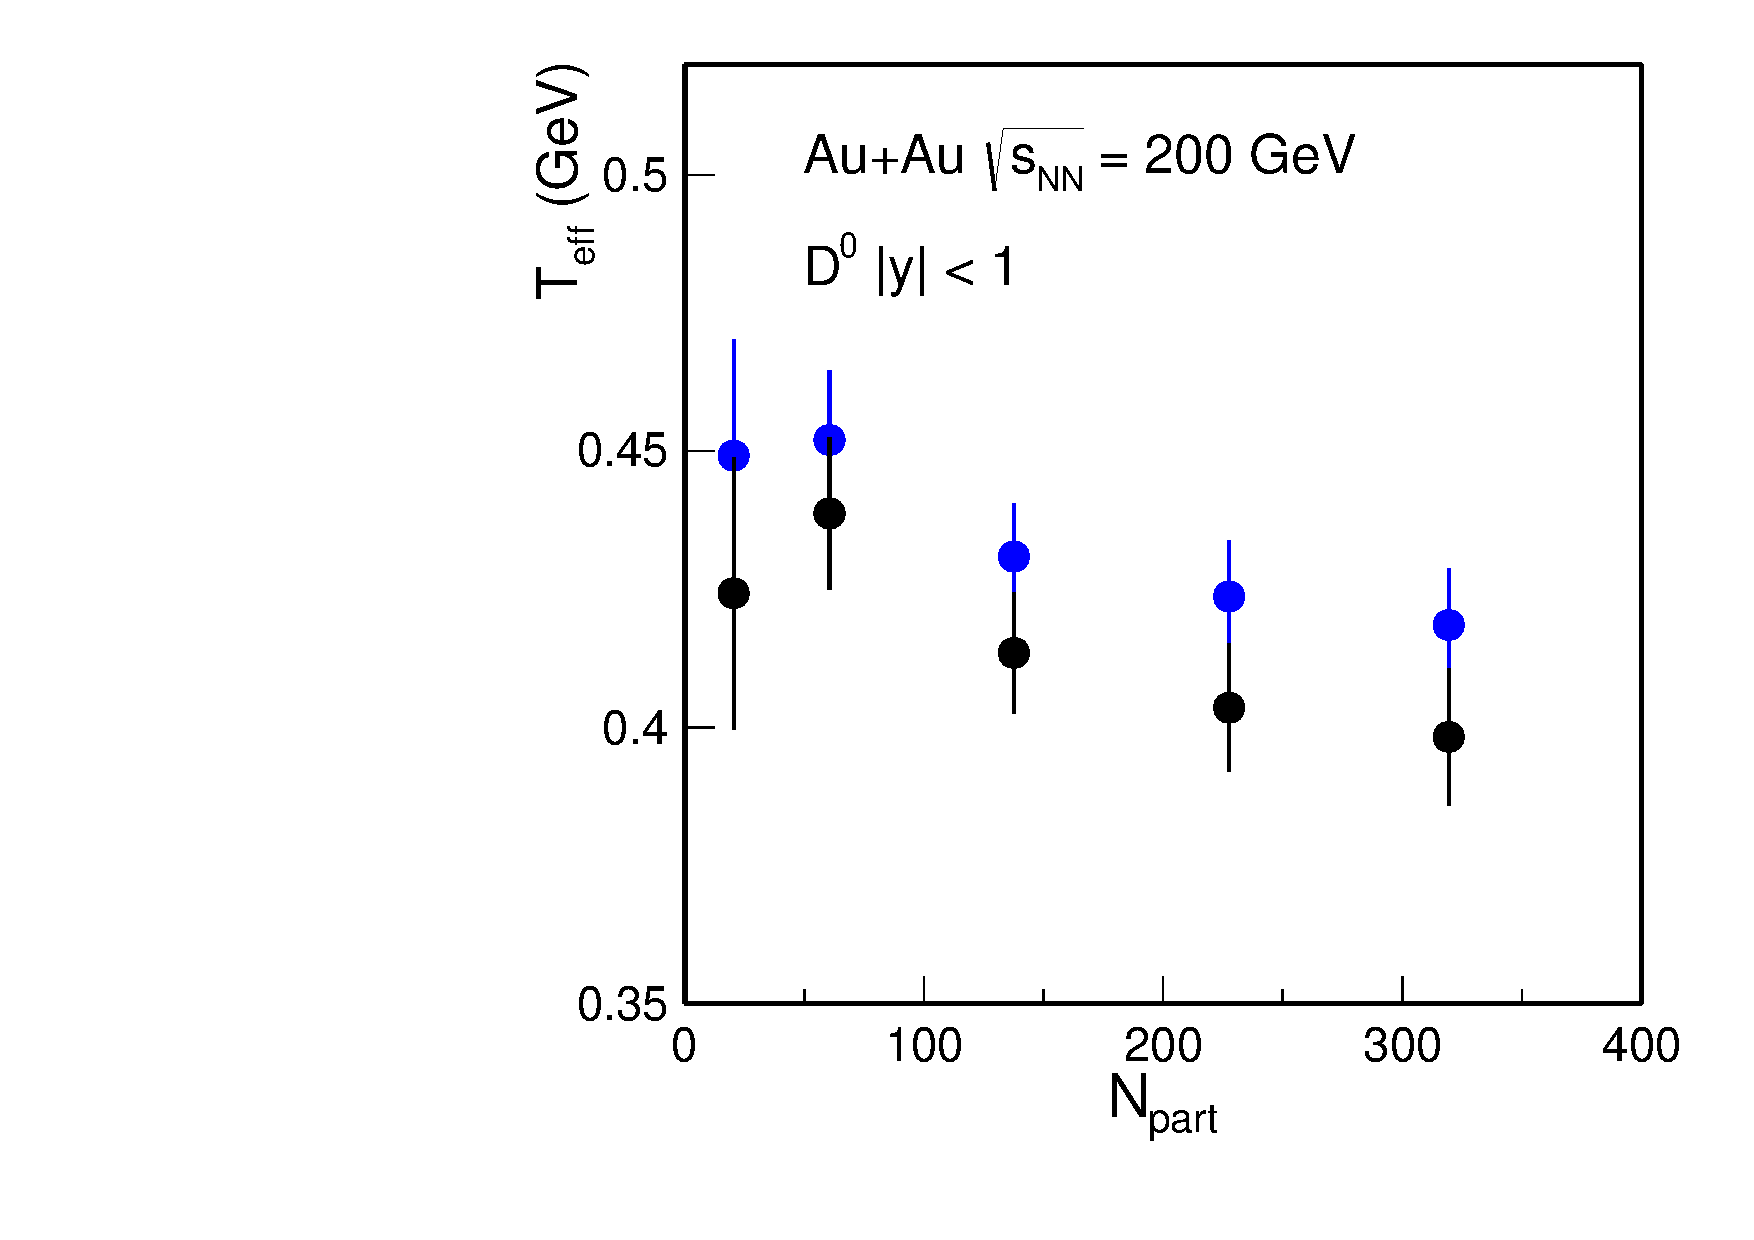
\includegraphics[width=0.48\textwidth]{fig/Teff_D0.pdf}
%DIF <  \caption{$T_{eff}$ vs. $N_{bin}$ for different centrality classes in Au + Au collisions at $\sqrt{s_{_{\rm NN}}}$ = 200\,GeV.}
%DIF >  \caption{$T_{eff}$ vs. $N_{bin}$ for different centrality classes in Au+Au collisions at ${\sqrt{s_{\rm NN}} = \rm{200\,GeV}}$.}
% \label{fig:Teff_D0} 
% \end{figure}

The obtained slope parameter $T_{\rm eff}$ for $D^0$ mesons is compared to other light and strange hadrons measured at RHIC. %Fig.~\ref{fig:mTFit_ALL} shows the exponential function fit to various hadron spectra 
\DIFdelbegin \DIFdel{Fig.}\DIFdelend \DIFaddbegin \DIFadd{Figure}\DIFaddend ~\ref{fig:Teff_ALL} summarizes the slope parameter $T_{\rm eff}$ for various identified hadrons ($\pi^{\pm}$, $K^{\pm}$, $p$/$\bar{p}$, $\phi$, $\Lambda$, $\Xi^-$, $\Omega$, $D^0$ and $J/\psi$) in central Au+Au collisions at \DIFdelbegin \DIFdel{$\sqrt{s_{_{\rm NN}}}$ = 200\,GeV}\DIFdelend \DIFaddbegin \DIFadd{$\sqrt{s_{_{\rm NN}}} {\rm = 200\,GeV}$}\DIFaddend . Point-by-point statistical and \DIFdelbegin \DIFdel{systematical uncertainties in the $m_{\rm T}$ spectra are added together in }\DIFdelend \DIFaddbegin \DIFadd{systematic uncertainties are added as a }\DIFaddend quadratic sum when performing these fits\DIFdelbegin \DIFdel{and error bars shown on the data points in this figure represent the total uncertainties}\DIFdelend . All fits are performed up to \DIFdelbegin \DIFdel{$m_{\rm T}$ - $m_{0}$ $<1$\,GeV/$c^2$ }\DIFdelend \DIFaddbegin \DIFadd{$m_{\rm T} - m_{0} <1\,\rm{GeV}/c^2$ }\DIFaddend ($\pi,\ K,\ p$), $<2$\,GeV/$c^2$ ($\phi,\ \Lambda,\ \Xi$), $<3$\,GeV/$c^2$($\Omega,\ D^{0},\ J/\psi$) for each particle\DIFaddbegin \DIFadd{, }\DIFaddend respectively. 

The slope parameter $T_{\rm eff}$ in a thermalized medium can be characterized by the random (generally interpreted as a kinetic freezeout temperature $T_{\rm fo}$) and collective (radial flow velocity $\langle\beta_{\rm T}\rangle$) components with a simple relation~\cite{StarWhitePaper,Csorgo:1995bi,Kolb:2003dz}\DIFdelbegin %DIFDELCMD < 

%DIFDELCMD < %%%
\[
\DIFdel{T_{\rm eff} = T_{\rm fo} + m_0 \langle\beta_{\rm T}\rangle^2
}\]
%DIFAUXCMD
%DIFDELCMD < 

%DIFDELCMD < %%%
\DIFdelend \DIFaddbegin \DIFadd{:
}\begin{equation}
  \DIFadd{\begin{aligned}
% \[
T_{\rm eff} = T_{\rm fo} + m_0 \langle\beta_{\rm T}\rangle^2,
% \end{aligned}
  }\end{equation}
\label{equ:equation7}
\]
\DIFaddend therefore, $T_{\rm eff}$ will show a linear dependence as a function of particle mass $m_0$ with a slope that can be used to characterize the radial flow collective velocity.

The data points \DIFdelbegin \DIFdel{show clearly }\DIFdelend \DIFaddbegin \DIFadd{clearly show }\DIFaddend two different systematic trends\DIFdelbegin \DIFdel{: }\DIFdelend \DIFaddbegin \DIFadd{. }\DIFaddend $\pi,\ K,\ p$ data points follow one linear dependence while $\phi,\ \Lambda,\ \Xi^{-},\ \Omega^{-},\ D^0$ data points follow another linear dependence, as represented by the dashed lines shown in Fig.~\ref{fig:Teff_ALL}. Particles, such as, $\pi,\ K,\ p$ gain radial collectivity through the whole system evolution, therefore the linear dependence exhibits a larger slope. On the other hand the linear dependence of $\phi,\ \Lambda,\ \Xi^{-},\ \Omega^{-},\ D^0$ data points shows a smaller slope indicating these particles may freeze out from the system earlier, and therefore receive less radial collectivity.

% \begin{figure}
% \centering
% 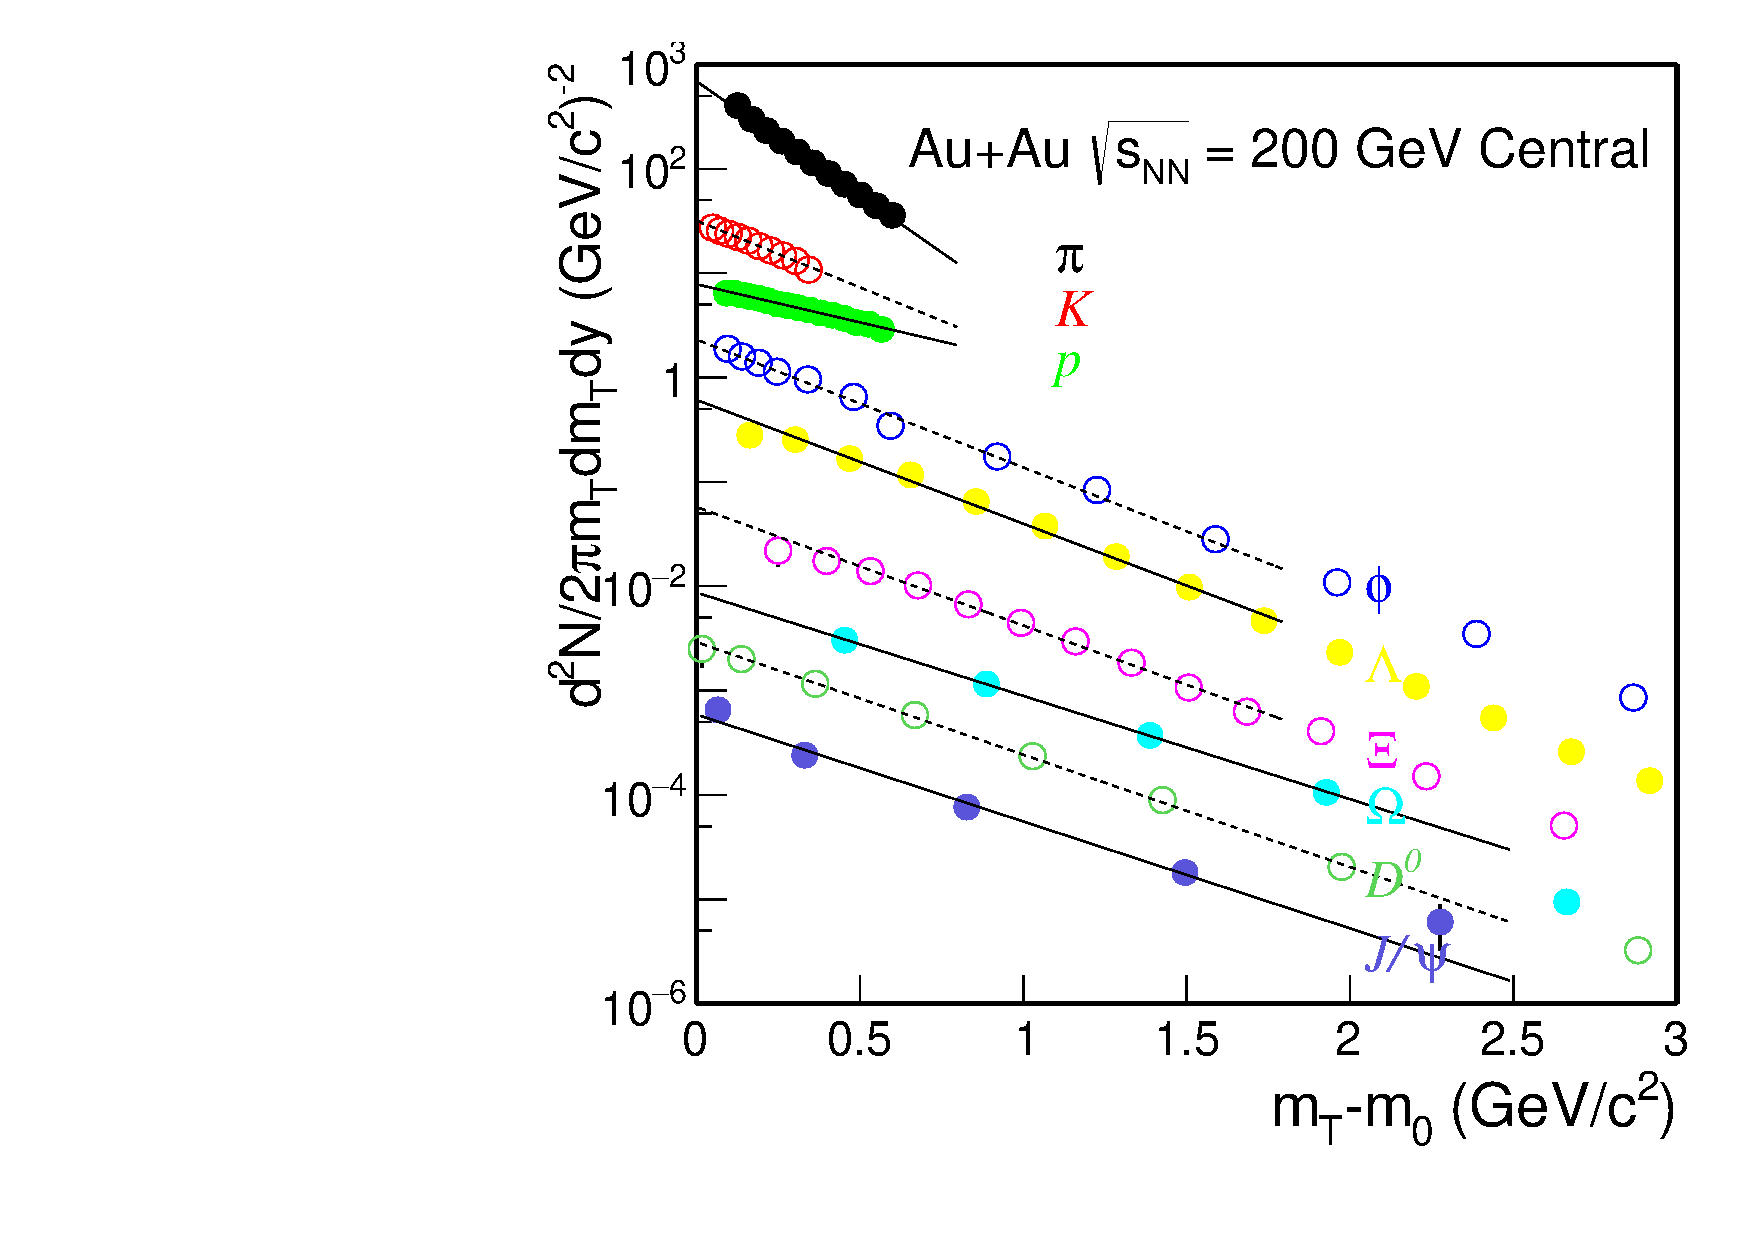
\includegraphics[width=0.5\textwidth]{fig/mTFit_ALL.pdf}
%DIF <  \caption{$D^{0}$ invariant yield at mid-rapidity ($|y|<1$) vs. ($m_{T}$ - $m_{0}$) for central collisions in Au + Au collisions at $\sqrt{s_{_{\rm NN}}}$ = 200\,GeV.}
%DIF >  \caption{$D^{0}$ invariant yield at mid-rapidity ($|y|<1$) vs. ($m_{T}$ - $m_{0}$) for central collisions in Au+Au collisions at ${\sqrt{s_{\rm NN}} = \rm{200\,GeV}}$.}
% \label{fig:mTFit_ALL} 
% \end{figure}

\begin{figure}
\centering
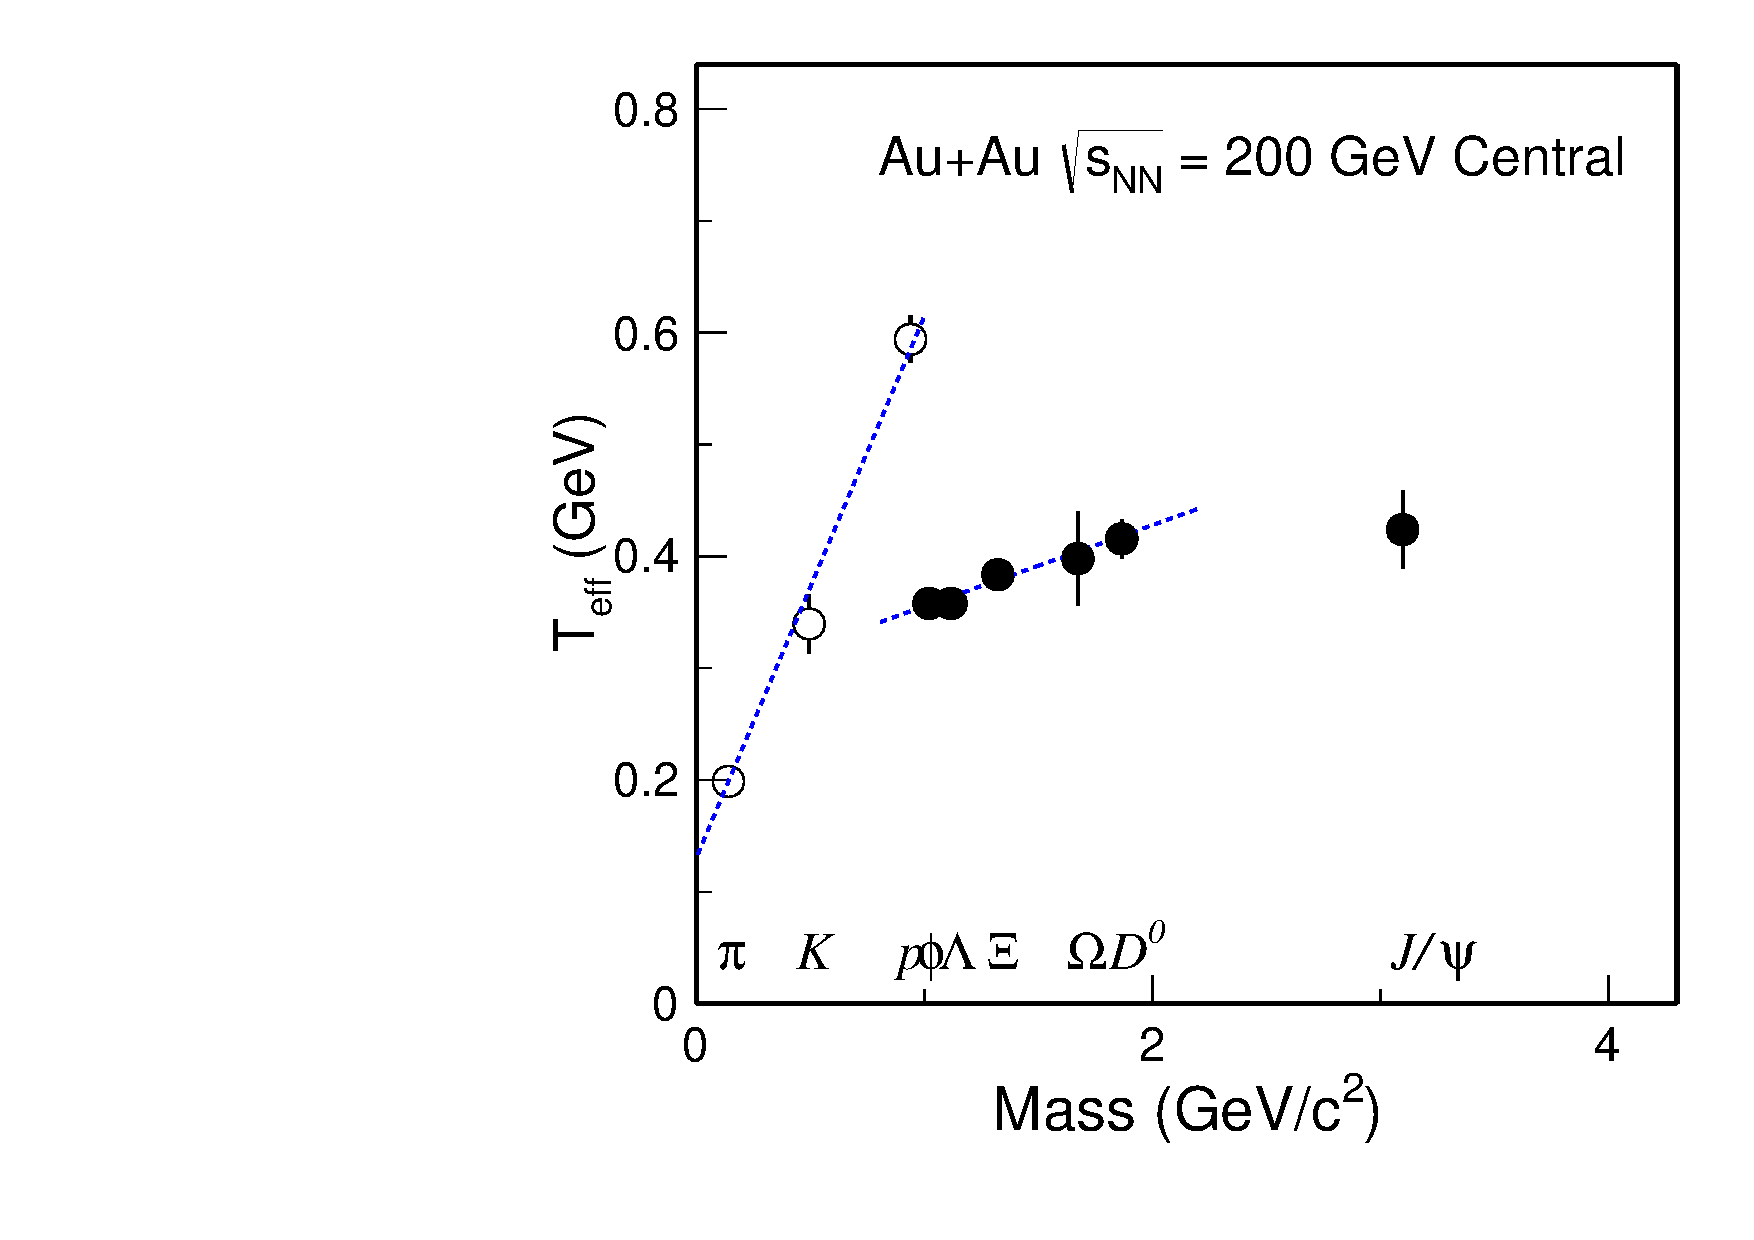
\includegraphics[width=0.43\textwidth]{fig/Teff_ALL.pdf}
% 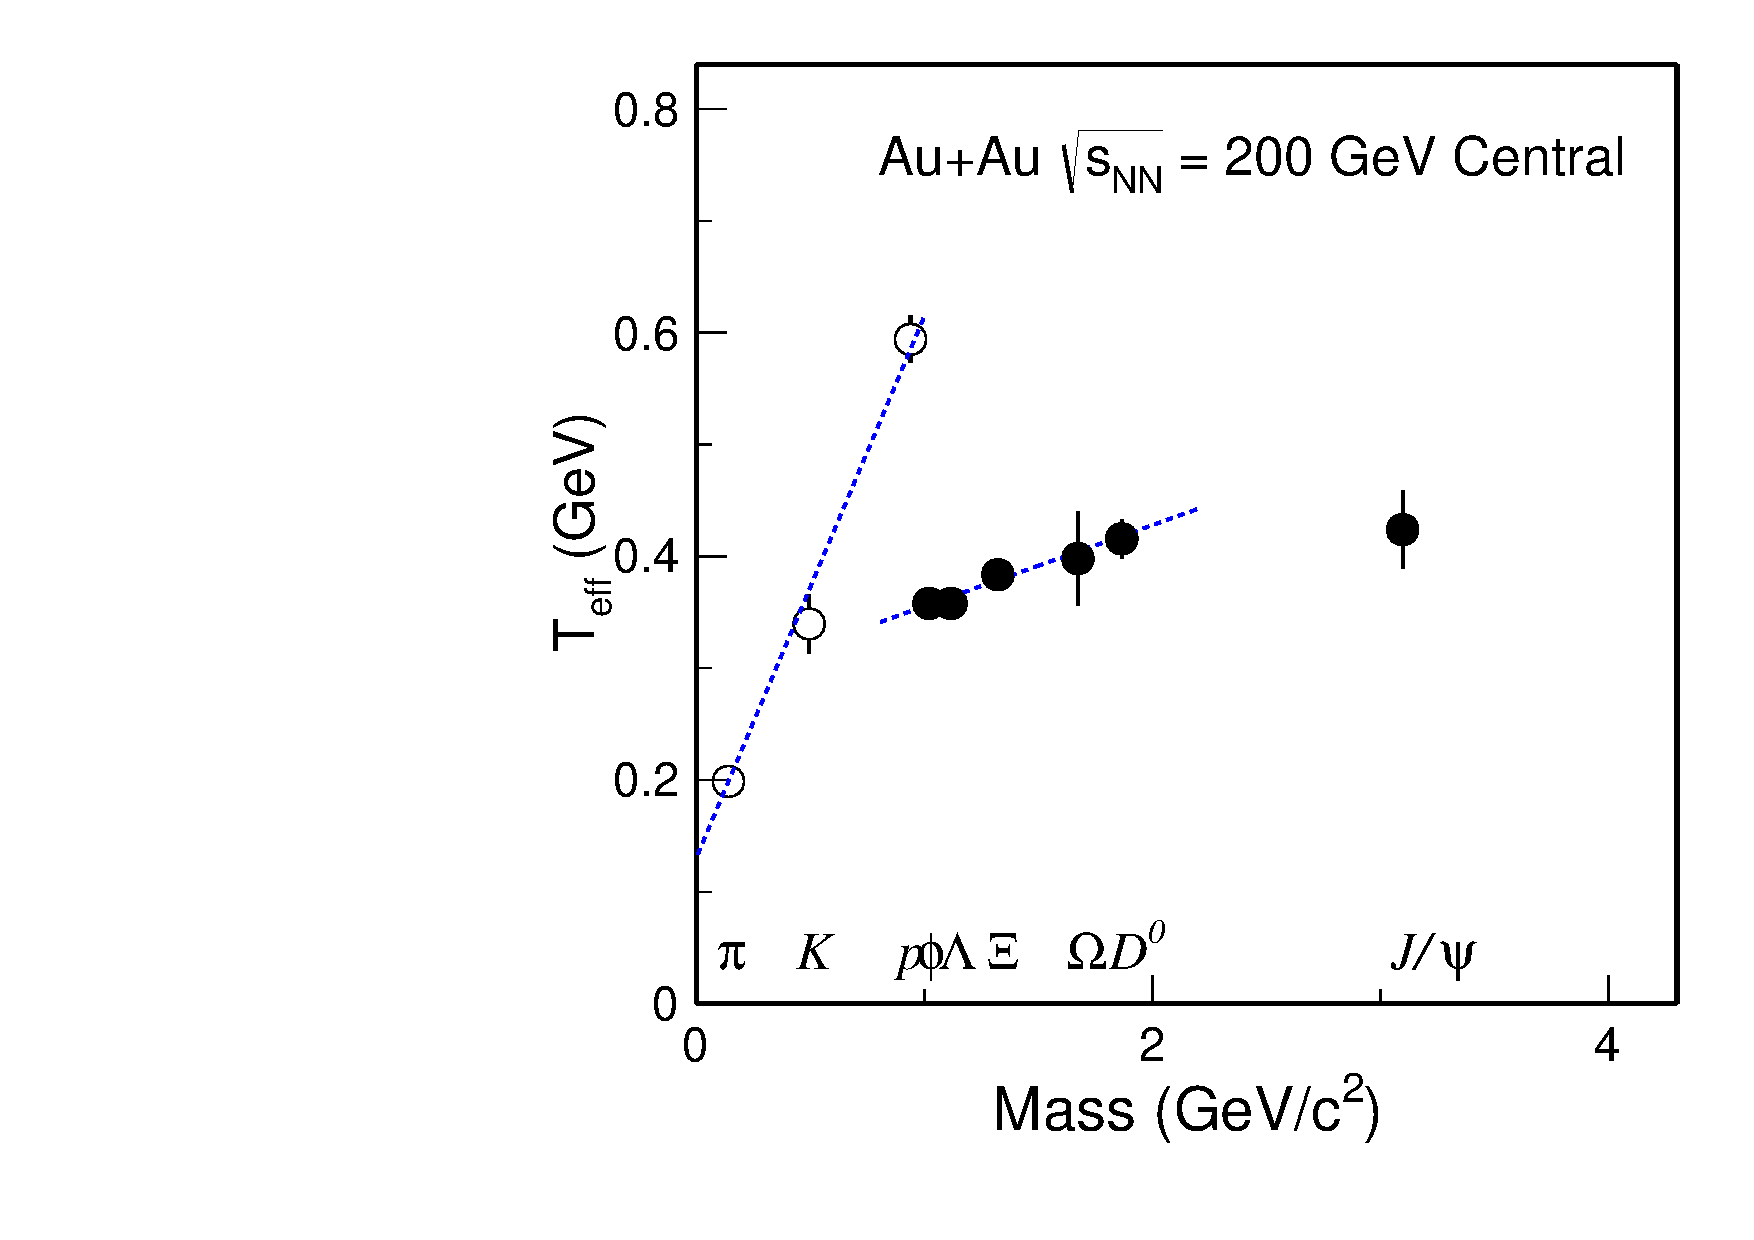
\includegraphics[width=0.4\textwidth]{fig/Teff_ALL.pdf}
\caption{Slope parameter $T_{\rm eff}$ for different particles in central Au+Au collisions\DIFdelbeginFL \DIFdelFL{at $\sqrt{s_{_{\rm NN}}}$ = 200\,GeV}\DIFdelendFL . The dashed lines depict linear function fits to $\pi,K,p$ and $\phi,\Lambda,\Xi^{-},\Omega^{-},D^0$ respectively.}
\label{fig:Teff_ALL} 
\end{figure}


\subsubsection{\DIFdelbegin %DIFDELCMD < %DIFDELCMD < \label{result:collectivity:BW}%%%
%%%
\DIFdelend Blast-wave fit}
\DIFaddbegin \label{result:collectivity:BW}
\DIFaddend 

\begin{figure}
\centering
\includegraphics[width=0.43\textwidth]{fig/BWFit.pdf}
% \includegraphics[width=0.4\textwidth]{fig/BWFit.pdf}
\caption{$D^{0}$ invariant yield at mid-rapidity ($|y|<1$) vs. transverse momentum for different centrality classes\DIFdelbeginFL \DIFdelFL{in Au + Au collisions at $\sqrt{s_{_{\rm NN}}}$ = 200\,GeV}\DIFdelendFL . \DIFdelbeginFL \DIFdelFL{Solid and dashed black }\DIFdelendFL \DIFaddbeginFL \DIFaddFL{Black }\DIFaddendFL lines depict Blast-Wave function and \DIFaddbeginFL \DIFaddFL{red lines are }\DIFaddendFL Tsallis Blast-Wave (TBW) fits.}
\label{fig:BWFit} 
\end{figure}

\DIFaddbegin \DIFadd{The }\DIFaddend Blast-Wave (BW) model is extensively used to study the particle kinetic freeze-out properties. Assuming a hard-sphere uniform particle source with a kinetic freeze-out temperature $T_{\rm kin}$ and a transverse radial flow velocity $\beta$, the particle transverse momentum spectral shape is given by~\cite{Schnedermann:1993ws}\DIFaddbegin \DIFadd{:
}\DIFaddend 

\DIFdelbegin %DIFDELCMD < \begin{widetext}
%DIFDELCMD < %%%
\[
\DIFdel{\frac{dN}{p_{\rm T}dp_{\rm T}} = \frac{dN}{m_{\rm T}dm_{\rm T}} \propto \int_0^R rdr m_{\rm T} I_0\bigg(\frac{p_{\rm T}\sinh\rho}{T_{\rm kin}}\bigg) K_1\bigg(\frac{m_{\rm T}\cosh\rho}{T_{\rm kin}}\bigg)
}\]
%DIFAUXCMD
%DIFDELCMD < \end{widetext}
%DIFDELCMD < %%%
\DIFdelend \DIFaddbegin \begin{equation}
  \DIFadd{\begin{aligned}
% \begin{widetext}
% \[
  & \frac{dN}{p_{T}dp_{T}} = \frac{dN}{m_{\rm T}dm_{\rm T}} \propto \\
  & \int_0^R rdr m_{\rm T} I_0\bigg(\frac{p_{T}\sinh\rho}{T_{\rm kin}}\bigg) K_1\bigg(\frac{m_{\rm T}\cosh\rho}{T_{\rm kin}}\bigg),
% \end{aligned}
%DIF >  \end{widetext}
  }\end{equation}
\label{equ:equation8}
\]
\DIFaddend where $\rho = \tanh^{-1}\beta$, and $I_0$ and $K_1$ are the modified Bessel functions. The flow velocity profile is taken as\DIFaddbegin \DIFadd{:
}\DIFaddend 

\DIFdelbegin \[
\DIFdel{\beta = \beta_{\rm S}\left(\frac{r}{R}\right)^{n}
}\]
%DIFAUXCMD
%DIFDELCMD < 

%DIFDELCMD < %%%
\DIFdelend \DIFaddbegin \begin{equation}
  \DIFadd{\begin{aligned}
% \[
\beta = \beta_{\rm S}\left(\frac{r}{R}\right)^{n},
% \]
  \end{aligned}
\label{equ:equation9}
}\end{equation}
\DIFaddend where $\beta_{\rm S}$ is the maximum velocity at the surface and $r/R$ is the relative radial position in the thermal source. The choice of $R$ only affects the overall spectrum magnitude while the spectrum shape constrains the three free parameters $T_{\rm kin}$, $\langle\beta\rangle=2/(2+n)\beta_{\rm S}$\DIFaddbegin \DIFadd{, }\DIFaddend and $n$.

% To account for the degree of non-equilibrium, Tsallis statistics has been introduced into the Blast-wave model with an additional parameter $q-1$~\cite{Tang:2008ud}, and the Blast-Wave distribution can be modified as
% \begin{widetext}
% \[
%DIF <  \frac{dN}{m_{\rm T}dm_{\rm T}} \propto m_{\rm T}\int_{-Y}^{+Y}\cosh(y)dy \int_{-\pi}^{+\pi} d\phi \int_0^R rdr \bigg(1+\frac{q-1}{T_{\rm kin}}\big(m_{\rm T}\cosh(y)\cosh(\rho)-p_{\rm T}\sinh(\rho)\cos(\phi)\big)\bigg)^{\textstyle -\frac{1}{q-1}}
%DIF >  \frac{dN}{m_{\rm T}dm_{\rm T}} \propto m_{\rm T}\int_{-Y}^{+Y}\cosh(y)dy \int_{-\pi}^{+\pi} d\phi \int_0^R rdr \bigg(1+\frac{q-1}{T_{\rm kin}}\big(m_{\rm T}\cosh(y)\cosh(\rho)-p_{T}\sinh(\rho)\cos(\phi)\big)\bigg)^{\textstyle -\frac{1}{q-1}}
% \]
% \end{widetext}
% In the limit of $q\rightarrow 1$, the TBW distribution returns to the regular Blast-Wave one. The new Tsallis Blast-Wave (TBW) model has been used to fit the RHIC light and strange hadron spectra and it shows nice description of these particle spectra up to 3 GeV/$c$.
%

Figure~\ref{fig:BWFit} shows the Blast-Wave and Tsallis Blast-Wave (TBW) \DIFdelbegin \DIFdel{~\mbox{%DIFAUXCMD
\cite{Tang:2008ud} }%DIFAUXCMD
}\DIFdelend fits to the data in different centrality bins\DIFdelbegin \DIFdel{, respectively}\DIFdelend . The $n$ parameter in these \DIFdelbegin \DIFdel{fit is }\DIFdelend \DIFaddbegin \DIFadd{fits are }\DIFaddend fixed to be 1 due to the limited number of data points and \DIFdelbegin \DIFdel{also }\DIFdelend \DIFaddbegin \DIFadd{is }\DIFaddend inspired by the fit result for \DIFdelbegin \DIFdel{light flavor }\DIFdelend \DIFaddbegin \DIFadd{light-flavor }\DIFaddend hadrons ($\pi,K,p$)\DIFdelbegin \DIFdel{. The $p_{\rm T}$ }\DIFdelend \DIFaddbegin \DIFadd{~\mbox{%DIFAUXCMD
\cite{Tang:2008ud}}%DIFAUXCMD
. The $p_{T}$ }\DIFaddend range in the BW fits is restricted to be less than 3$m_{0}$ where $m_{0}$ is the rest mass of $D^0$ mesons.

\begin{figure}
\centering
\includegraphics[width=0.43\textwidth]{fig/TvsBeta.pdf}
\caption{\DIFaddbeginFL \DIFaddFL{Results of }\DIFaddendFL $T_{\rm kin}$ vs. $\langle\beta\rangle$ from the Blast-Wave model fits to different groups of particles. The data points for each group of particles present the results from different centrality bins with the most central data point at the largest $\langle\beta\rangle$.}
\label{fig:BWFitSummary} 
\end{figure}

Figure~\ref{fig:BWFitSummary} summarizes the fit parameters $T_{\rm kin}$ vs. $\langle\beta\rangle$ from the Blast-Wave model fits to different \DIFdelbegin \DIFdel{group }\DIFdelend \DIFaddbegin \DIFadd{groups }\DIFaddend of particles: black markers for the simultaneous fit to $\pi,\ K,\ p$\DIFdelbegin \DIFdel{, }\DIFdelend \DIFaddbegin \DIFadd{; }\DIFaddend red markers for the simultaneous fit to $\phi,\ \Xi^-$ and blue markers for the fit to $D^0$. The data points for each group of particles represent the fit results from different centrality bins with the most central data point at the largest $\langle\beta\rangle$ value. Similar as in the fit to \DIFaddbegin \DIFadd{the }\DIFaddend $m_{\rm T}$ spectra, point-by-point statistical and \DIFdelbegin \DIFdel{systematical uncertainties on the measured $p_{\rm T}$ spectra }\DIFdelend \DIFaddbegin \DIFadd{systematic uncertainties }\DIFaddend are added in \DIFdelbegin \DIFdel{quadratic }\DIFdelend \DIFaddbegin \DIFadd{quadrature }\DIFaddend when performing the fit. The fit results for $\pi,\ K,\ p$ are consistent with previously published results~\cite{Tang:2008ud}. The fit results for multi-strangeness particles $\phi,\ \Xi^{-}$ and $D^0$ show much smaller mean transverse velocity $\langle\beta\rangle$ and larger kinetic freeze-out temperature. \DIFdelbegin \DIFdel{This is also consistent with that these particles freeze out }\DIFdelend \DIFaddbegin \DIFadd{Which is consistent with particle freeze out earlier }\DIFaddend from the system \DIFdelbegin \DIFdel{earlier }\DIFdelend and gain less radial collectivity. The resulting $T_{\rm kin}$ parameters for $\phi,\ \Xi^-$ and for $D^0$ are close to the critical temperature $T_{\rm C}$ (\DIFaddbegin \DIFadd{likely, }\DIFaddend of about 160 MeV) indicating negligible contribution from the hadronic stage to the observed radial flow of these particles. The collectivity they obtain \DIFdelbegin \DIFdel{are }\DIFdelend \DIFaddbegin \DIFadd{is }\DIFaddend mostly through the partonic stage re-scatterings in the QGP phase. 

The TBW fit accounts for non-equilibrium \DIFdelbegin \DIFdel{feature }\DIFdelend \DIFaddbegin \DIFadd{features }\DIFaddend in a system with an additional parameter $q$~\cite{Tang:2008ud}. %DIF < Table~\ref{table:TBW_fit} 
\DIFdelbegin \DIFdel{TableVI }\DIFdelend \DIFaddbegin \DIFadd{Table~\ref{table:TBW_fit} }\DIFaddend lists the fitting parameters, $\langle\beta\rangle$ and $(q-1)$ for the $D^0$ data in different centralities. Results show a similar trend as the regular BW fit, i.e. the most central data point \DIFdelbegin \DIFdel{locates }\DIFdelend \DIFaddbegin \DIFadd{is located }\DIFaddend at the largest $\langle\beta\rangle$ value. The $(q-1)$ parameter in TBW, which characterizes the degree of non-equilibrium in a system, indicates \DIFaddbegin \DIFadd{a }\DIFaddend decreasing trend from peripheral to central collisions, indicating that the system is approaching \DIFdelbegin \DIFdel{towards }\DIFdelend thermalization in more central collisions.
% Qualitatively, increasing centrality produces a strong increase in flow velocity, a mild increase in temperature, and a dramatic decrease in (q−1). This is consistent with a picture of increased thermalization with centrality but disfavors complete thermal equilibrium in all systems.

\begin{table}[t]
\DIFdelbeginFL %DIFDELCMD < \centering{
%DIFDELCMD <   \caption{ $\langle\beta\rangle$ and $(q-1)$ from the Tsallis Blast-Wave fits to the $D^0$ data in different centralities .}
%DIFDELCMD < \begin{tabular}{rcccccccc} \hline \hline
%DIFDELCMD <   \hspace{1cm}Centrality\hspace{1cm} & \multicolumn{3}{c}{$\langle\beta\rangle$($c$)} & & \multicolumn{3}{c}{$q-1$} & \hspace{1cm} \\ \hline
%DIFDELCMD <   0--10 \%\hspace{1cm}     & 0.263 & $\pm$ & 0.018 & & 0.066 & $\pm$ & 0.008 \\
%DIFDELCMD <   10--20 \%\hspace{1cm}    & 0.255 & $\pm$ & 0.022 & & 0.068 & $\pm$ & 0.010 \\
%DIFDELCMD <   20--40 \%\hspace{1cm}    & 0.264 & $\pm$ & 0.015 & & 0.070 & $\pm$ & 0.007 \\
%DIFDELCMD <   40--60 \%\hspace{1cm}    & 0.251 & $\pm$ & 0.023 & & 0.074 & $\pm$ & 0.011 \\
%DIFDELCMD <   60--80 \%\hspace{1cm}    & 0.217 & $\pm$ & 0.037 & & 0.075 & $\pm$ & 0.010  \\ \hline \hline
%DIFDELCMD < \end{tabular}
%DIFDELCMD < }
%DIFDELCMD < \label{table:TBW_fit}
%DIFDELCMD < %%%
\DIFdelendFL \DIFaddbeginFL \centering{
  \caption{ $\langle\beta\rangle$ and $(q-1)$ from the Tsallis Blast-Wave fits to the $D^0$ data in different centralities .}
\begin{tabular}{rcccccccc} \hline \hline
  \hspace{1cm}Centrality\hspace{1cm} & \multicolumn{3}{c}{$\langle\beta\rangle$($c$)} & & \multicolumn{3}{c}{$q-1$} & \hspace{1cm} \\ \hline
  0--10 \%\hspace{1cm}     & 0.263 & $\pm$ & 0.018 & & 0.066 & $\pm$ & 0.008 \\
  10--20 \%\hspace{1cm}    & 0.255 & $\pm$ & 0.022 & & 0.068 & $\pm$ & 0.010 \\
  20--40 \%\hspace{1cm}    & 0.264 & $\pm$ & 0.015 & & 0.070 & $\pm$ & 0.007 \\
  40--60 \%\hspace{1cm}    & 0.251 & $\pm$ & 0.023 & & 0.074 & $\pm$ & 0.011 \\
  60--80 \%\hspace{1cm}    & 0.217 & $\pm$ & 0.037 & & 0.075 & $\pm$ & 0.010  \\ \hline \hline
\end{tabular}
\label{table:TBW_fit}
}
\DIFaddendFL \end{table}

\subsection{\DIFdelbegin %DIFDELCMD < %DIFDELCMD < \label{result:RCP}%%%
%%%
\DIFdelend Nuclear Modification Factor - $R_{\rm CP}$ \DIFdelbegin \DIFdel{$\&\&$  }\DIFdelend \DIFaddbegin \DIFadd{and }\DIFaddend $R_{\rm AA}$}
\DIFaddbegin \label{result:RCP}
\DIFaddend 

\begin{figure}
\centering
\includegraphics[width=0.45\textwidth]{fig/D0_Rcp1.pdf}
\caption{$D^{0}$ $R_{\rm CP}$ with the 60--80\% spectrum as the reference for different centrality classes in Au+Au collisions \DIFdelbeginFL \DIFdelFL{at $\sqrt{s_{_{\rm NN}}}$ = 200\,GeV }\DIFdelendFL compared to that of other light and strange mesons ($\pi^{\pm}$, $K^0_{S}$ and $\phi$)~\cite{Adams2006_Identified,Abelev2009,Agakishiev2012}. The statistical and systematic uncertainties are shown as error bars and brackets on the data points. The grey bands around unity depict the systematic uncertainty due to vertex resolution correction, mostly from the 60--80\% reference spectrum. The light and dark green boxes on the right depict the normalization uncertainty in determining the $N_{\rm bin}$.}
\label{fig:D0_Rcp} 
\end{figure}

Figure~\ref{fig:D0_Rcp} shows the calculated $R_{\rm CP}$ with the 60--80\% peripheral bin as the reference for different centrality bins 0--10\%, 10--20\%, 20--40\% and 40--60\% and \DIFaddbegin \DIFadd{is }\DIFaddend compared to other light and strange flavor mesons. The grey bands around unity depict the vertex resolution correction uncertainty on the measured $D^0$ data points, mostly originating from the 60--80\% reference spectrum. The dark and light green boxes around unity on the right side indicate the global $N_{\rm bin}$ systematic uncertainties for the 60--80\% centrality bin and for the corresponding centrality bin in each panel. The global $N_{\rm bin}$ systematic uncertainties should be applied to the data points of all particles in each panel.

The measured $D^0$ $R_{\rm CP}$ in central 0--10\% collisions shows a significant suppression at \DIFdelbegin \DIFdel{$p_{\rm T}>$ }\DIFdelend \DIFaddbegin \DIFadd{$p_{T}>$ }\DIFaddend 5\,GeV/$c$. The suppression level is similar to that of light and strange flavor mesons and the $R_{\rm CP}$ suppression gradually \DIFdelbegin \DIFdel{descreses }\DIFdelend \DIFaddbegin \DIFadd{decreases }\DIFaddend when moving towards \DIFaddbegin \DIFadd{from central collisions to }\DIFaddend mid-central and peripheral collisions. \DIFdelbegin \DIFdel{At $p_{\rm T}<4$}\DIFdelend \DIFaddbegin \DIFadd{The $D^0$ $R_{\rm CP}$ for $p_{T}<4$}\DIFaddend \,GeV/$c$ \DIFdelbegin \DIFdel{, the $D^0$ $R_{\rm CP}$ is higher than those of light flavor hadrons$\pi^{\pm}$ and $K_{S}^0$}\DIFdelend \DIFaddbegin \DIFadd{is consistent with no suppression, in contrast to light-flavor hadrons}\DIFaddend . This structure is consistent with the expectation from model predictions that charm quarks gain sizable \DIFdelbegin \DIFdel{collectivity }\DIFdelend \DIFaddbegin \DIFadd{collective motion }\DIFaddend during the medium evolution. Comparisons to dynamic model calculations for the $D^0$ $R_{\rm CP}$ will be discussed in the next \DIFdelbegin \DIFdel{section.}\DIFdelend \DIFaddbegin \DIFadd{Sec.~\ref{result:theory}.
}\DIFaddend 

\begin{figure}
\centering
\includegraphics[width=0.45\textwidth]{fig/D0_Rcp2.pdf}
\caption{$D^{0}$ $R_{\rm CP}$ with the 40--60\% spectrum as the reference for different centrality classes in Au+Au collisions \DIFdelbeginFL \DIFdelFL{at $\sqrt{s_{_{\rm NN}}}$ = 200\,GeV }\DIFdelendFL compared to that of other light and strange mesons ($\pi^{\pm}$, $K^0_{S}$ and $\phi$)~\cite{Adams2006_Identified,Abelev2009,Agakishiev2012}. The statistical and systematic uncertainties are shown as error bars and brackets on the data points. The grey bands around unity depict the systematic uncertainty due to vertex resolution correction, mostly from the 40--60\% reference spectrum. The light and dark green boxes on the right depict the normalization uncertainty in determining the $N_{\rm bin}$.}
\label{fig:D0_Rcp2} 
\end{figure}

The precision of \DIFaddbegin \DIFadd{the }\DIFaddend 60--80\% centrality spectrum is limited due to the large systematic uncertainty in determining the $N_{\rm bin}$ based on the MC Glauber model. \DIFdelbegin \DIFdel{Fig.}\DIFdelend \DIFaddbegin \DIFadd{Figure}\DIFaddend ~\ref{fig:D0_Rcp2} shows the $D^0$ $R_{\rm CP}$ for different centralities as a function of \DIFdelbegin \DIFdel{$p_{\rm T}$ }\DIFdelend \DIFaddbegin \DIFadd{$p_{T}$ }\DIFaddend with the 40--60\% centrality spectrum as the reference. The grey band around unity in the top panel is the vertex contribution for the systematic uncertainties from the 40--60\% centrality. The green boxes around unity depict the global $N_{\rm bin}$ systematic uncertainties for the 40--60\% centrality bin and for each corresponding centrality bin. As a comparison, $R_{\rm CP}$ of charged pions, $K_{s}^{0}$ and $\phi$ in the corresponding centralities are also plotted in each panel. With much smaller systematic uncertainties, the observations seen before using the 60--80\% centrality spectrum as the reference still hold. 


% \begin{figure}
% \centering
% \includegraphics[width=0.48\textwidth]{fig/Rcp_Nbin_D0_2.pdf}
%DIF <  \caption{$D^{0}$ $R_{cp}$ vs. $N_{bin}$ in Au + Au collisions.}
%DIF >  \caption{$D^{0}$ $R_{cp}$ vs. $N_{bin}$ in Au+Au collisions.}
% \label{fig/Rcp_Nbin_D0_2} 
% \end{figure}

\begin{figure}
\centering
\includegraphics[width=0.45\textwidth]{fig/D0_RAA.eps}
%DIF <  \caption{$D^{0}$ $R_{\rm AA}$ with the $p+p$ spectrum as the reference for different centrality classes in Au + Au collisions at $\sqrt{s_{_{\rm NN}}}$ = 200\,GeV. The first two and last two data points are empty circles indicating that those are unmeasured $p_{\rm T}$ range from $p+p$. The statistical and systematic uncertainties are shown as error bars and brackets on the data points for Au + Au. The grey bands around each data point depict the systematic uncertainty from $p+p$ reference spectrum. The light and dark green boxes on the right depict the normalization uncertainty in determining the $N_{\rm bin}$ and cross section from $p+p$.}
%DIF >  \caption{$D^{0}$ $R_{\rm AA}$ with the $p$+$p$ spectrum as the reference for different centrality classes in Au+Au collisions at ${\sqrt{s_{\rm NN}} = \rm{200\,GeV}}$. The first two and last two data points are empty circles indicating that those are unmeasured $p_{T}$ range from $p$+$p$. The statistical and systematic uncertainties are shown as error bars and brackets on the data points for Au+Au. The grey bands around each data point depict the systematic uncertainty from $p$+$p$ reference spectrum. The light and dark green boxes on the right depict the normalization uncertainty in determining the $N_{\rm bin}$ and cross section from $p$+$p$.}
\caption{$D^{0}$ $R_{\rm AA}$ with the \DIFdelbeginFL \DIFdelFL{$p+p$ }\DIFdelendFL \DIFaddbeginFL \DIFaddFL{$p$+$p$ }\DIFaddendFL spectrum as the reference for different centrality classes\DIFdelbeginFL \DIFdelFL{in Au + Au collisions at $\sqrt{s_{_{\rm NN}}}$ = 200\,GeV}\DIFdelendFL . The first two and last two data points are presented as empty circles, indicating that the \DIFdelbeginFL \DIFdelFL{$p+p$ }\DIFdelendFL \DIFaddbeginFL \DIFaddFL{$p$+$p$ }\DIFaddendFL reference is extrapolated into these $p_T$ ranges. The statistical and systematic uncertainties are shown as error bars and brackets on the data points. The light and dark green boxes on the right depict the normalization uncertainty in determining the $N_{\rm bin}$ and cross \DIFdelbeginFL \DIFdelFL{section }\DIFdelendFL \DIFaddbeginFL \DIFaddFL{sectional }\DIFaddendFL from \DIFdelbeginFL \DIFdelFL{$p+p$}\DIFdelendFL \DIFaddbeginFL \DIFaddFL{$p$+$p$}\DIFaddendFL .}
\label{fig:D0_RAA} 
\end{figure}

\begin{figure}
\centering
\includegraphics[width=0.45\textwidth]{fig/D0_RAA_LHC.pdf}
  \caption{$D^{0}$ $R_{\rm AA}$ in most central (0-10\%) Au+Au collisions at \DIFdelbeginFL \DIFdelFL{$\sqrt{s_{_{\rm NN}}}$ = 200\,GeV}\DIFdelendFL \DIFaddbeginFL \DIFaddFL{${\sqrt{s_{\rm NN}} = \rm{200\,GeV}}$}\DIFaddendFL , comparison to ALICE \DIFdelbeginFL \DIFdelFL{D }\DIFdelendFL \DIFaddbeginFL \DIFaddFL{$D$ }\DIFaddendFL meson result in most central (0-10\%) Pb + Pb collisions at $\sqrt{s_{_{\rm NN}}}$ = 2.76\,TeV, and hadron from ALICE and $\pi^{\pm}$ from STAR. Also compared to model calculations \DIFaddbeginFL \DIFaddFL{from LBT and Duke group}\DIFaddendFL ~\DIFdelbeginFL \DIFdelFL{\mbox{%DIFAUXCMD
\cite{Cao:2016gvr,LBT:private}}%DIFAUXCMD
}\DIFdelendFL \DIFaddbeginFL \DIFaddFL{\mbox{%DIFAUXCMD
\cite{Cao:2016gvr,LBT:private,Xu:2017obm}}%DIFAUXCMD
}\DIFaddendFL . The statistical and systematic uncertainties are similar as \DIFaddbeginFL \DIFaddFL{in }\DIFaddendFL previous plots.}
\label{fig:D0_RAA_LHC} 
\end{figure}

Figure~\ref{fig:D0_RAA} shows the calculated $R_{\rm AA}$ with the \DIFdelbegin \DIFdel{$p+p$ }\DIFdelend \DIFaddbegin \DIFadd{$p$+$p$ }\DIFaddend measurement ~\cite{Star_D_pp} as the reference for different centrality bins 0--10\% (a), 10--40\% (b) and 40--80\% (c) and compared with the previous \DIFaddbegin \DIFadd{Au+Au }\DIFaddend measurements using the STAR TPC after the recent correction~\DIFdelbegin \DIFdel{\mbox{%DIFAUXCMD
\cite{Star_D_RAA_corr}}%DIFAUXCMD
. The $p+p$ }\DIFdelend \DIFaddbegin \DIFadd{\mbox{%DIFAUXCMD
\cite{Star_D_RAA}}%DIFAUXCMD
. The $p$+$p$ }\DIFaddend $D^0$ reference spectrum is updated using the latest global analysis of charm fragmentation ratios from~\cite{charm_frag} and also by taking into account the $p_T$ dependence of the fragmentation ratio between $D^0$ and \DIFdelbegin \DIFdel{$D^∗_\pm$ }\DIFdelend \DIFaddbegin \DIFadd{$D^{*\pm}$ }\DIFaddend from PYTHIA. The new measurement with the HFT detector shows a nice agreement with the measurement without the HFT, but with much improved precision. The grey bands around each data point depict the \DIFdelbegin \DIFdel{$p+p$ }\DIFdelend \DIFaddbegin \DIFadd{$p$+$p$ }\DIFaddend systematic uncertainty on the measured $D^0$ data points. The first two and last two data points are empty circles indicating those are \DIFdelbegin \DIFdel{extrapolated $p+p$ }\DIFdelend \DIFaddbegin \DIFadd{calculated with an extrapolated $p$+$p$ }\DIFaddend reference. The dark and light green boxes around unity on the right side indicate the global $N_{\rm bin}$ systematic uncertainties for the corresponding centrality bin in each panel and the global cross \DIFdelbegin \DIFdel{section uncertainties from $p+p$}\DIFdelend \DIFaddbegin \DIFadd{sectional uncertainties from $p$+$p$}\DIFaddend .

The measured $D^0$ $R_{\rm AA}$ in central (0-10\%) and mid-central (10-40\%) collisions show a significant suppression at the high \DIFdelbegin \DIFdel{$p_{\rm T}$ }\DIFdelend \DIFaddbegin \DIFadd{$p_{T}$ }\DIFaddend range which reaffirms the strong interactions between charm quarks and the medium, while the new Au+Au data points from this analysis contain much improved precision. \DIFdelbegin \DIFdel{Fig.}\DIFdelend \DIFaddbegin \DIFadd{Figure}\DIFaddend ~\ref{fig:D0_RAA_LHC} shows the $D^0$ $R_{\rm AA}$ in the 0-10\% most central collisions compared to that of \DIFdelbegin \DIFdel{average D }\DIFdelend \DIFaddbegin \DIFadd{(a) average $D$ }\DIFaddend meson from ALICE \DIFdelbegin \DIFdel{(a) and }\DIFdelend \DIFaddbegin \DIFadd{and (b) }\DIFaddend charged hadron from ALICE and $\pi^{\pm}$ from STAR\DIFdelbegin \DIFdel{(b)}\DIFdelend ~\cite{Alice_D_RAA_2,Alice_hadron_RAA,PhenixPi0}. The comparison of $D^0$ \DIFaddbegin \DIFadd{suppression }\DIFaddend between STAR and ALICE shows reasonable agreement within the uncertainties despite the large energy difference from 200\,GeV to 2.76\,TeV. The comparison to that of light hadrons shows similar suppression at the high \DIFdelbegin \DIFdel{$p_{\rm T}$}\DIFdelend \DIFaddbegin \DIFadd{$p_{T}$}\DIFaddend , while in the \DIFdelbegin \DIFdel{intermedium }\DIFdelend \DIFaddbegin \DIFadd{intermediate }\DIFaddend range, $D^0$ mesons are less suppressed.



\DIFdelbegin %DIFDELCMD < \begin{figure}
%DIFDELCMD < \centering
%DIFDELCMD < \includegraphics[width=0.45\textwidth]{fig/D0_Rcp11.pdf}
%DIFDELCMD < %%%
%DIFDELCMD < \caption{%
{%DIFAUXCMD
\DIFdelFL{$D^{0}$ $R_{\rm CP}$ with the 60--80\% spectrum as the reference for different centrality classes in Au + Au collisions compared to model calculations~\mbox{%DIFAUXCMD
\cite{Cao:2016gvr,LBT:private}}%DIFAUXCMD
. The statistical and systematic uncertainties are shown as error bars and brackets on the data points. The grey bands around unity depict the systematic uncertainty due to vertex resolution correction, mostly from the 60--80\% reference spectrum. The light and dark green boxes on the right depict the normalization uncertainty in determining the $N_{\rm bin}$.}}
%DIFAUXCMD
%DIFDELCMD < \label{fig:D0_Rcp11} 
%DIFDELCMD < \end{figure}
%DIFDELCMD < 

%DIFDELCMD < \begin{figure}
%DIFDELCMD < \centering
%DIFDELCMD < \includegraphics[width=0.45\textwidth]{fig/D0_Rcp22.pdf}
%DIFDELCMD < %%%
%DIFDELCMD < \caption{%
{%DIFAUXCMD
\DIFdelFL{$D^{0}$ $R_{\rm CP}$ with the 40--60\% spectrum as the reference for different centrality classes in Au + Au collisions compared to model calculations~\mbox{%DIFAUXCMD
\cite{Cao:2016gvr,LBT:private,Xu:2017obm}}%DIFAUXCMD
. The statistical and systematic uncertainties are shown as error bars and brackets on the data points. The grey bands around unity depict the systematic uncertainty due to vertex resolution correction, mostly from the 40--60\% reference spectrum. The light and dark green boxes on the right depict the normalization uncertainty in determining the $N_{\rm bin}$.}}
%DIFAUXCMD
%DIFDELCMD < \label{fig:D0_Rcp22} 
%DIFDELCMD < \end{figure}
%DIFDELCMD < 

%DIFDELCMD < %%%
\DIFdelend % \begin{figure*}
% \centering
% \includegraphics[width=0.8\textwidth]{fig/Rcp_Nbin_D0.pdf}
%DIF <  \caption{Integrated $D^{0}$ $R_{\rm CP}$ vs. $N_{\rm part}$ for $p_{\rm T}>$ 0\,GeV/$c$ (top) and $p_{\rm T}>$ 4\,GeV/$c$ (bottom), and for 60--80\% reference (left) and 40--60\% reference (right) respectively in Au + Au collisions at $\sqrt{s_{_{\rm NN}}}$ = 200\,GeV. Brackets depict the systematic uncertainties and colored lines represent model calculations from LBT and Duke groups.}
%DIF >  \caption{Integrated $D^{0}$ $R_{\rm CP}$ vs. $N_{\rm part}$ for $p_{T}>$ 0\,GeV/$c$ (top) and $p_{T}>$ 4\,GeV/$c$ (bottom), and for 60--80\% reference (left) and 40--60\% reference (right) respectively in Au+Au collisions at ${\sqrt{s_{\rm NN}} = \rm{200\,GeV}}$. Brackets depict the systematic uncertainties and colored lines represent model calculations from LBT and Duke groups.}
% \label{fig:Rcp_Nbin_D0} 
% \end{figure*}

\subsection{\DIFdelbegin %DIFDELCMD < %DIFDELCMD < \label{result:D0barD0ratio} %%%
%%%
\DIFdelend $\overline{D}^{0}$ and $D^{0}$ spectra and double ratio}
\DIFaddbegin \label{result:D0barD0ratio} 
\DIFaddend 

\begin{figure}
\centering
\includegraphics[width=0.45\textwidth]{fig/D0_spectra_bothposneg.pdf}
\caption{$D^{0}$ and $\overline{D}^{0}$ invariant yield at mid-rapidity ($|y|<1$) vs. transverse momentum for different centrality classes\DIFdelbeginFL \DIFdelFL{in Au + Au collisions at $\sqrt{s_{_{\rm NN}}}$ = 200\,GeV}\DIFdelendFL . Error bars (not visible for many data points) indicate statistical uncertainties and brackets depict \DIFdelbeginFL \DIFdelFL{systematical }\DIFdelendFL \DIFaddbeginFL \DIFaddFL{systematic }\DIFaddendFL uncertainties. Global systematic uncertainties in $B.R.$ and $N_{\rm bin}$ are not plotted. Solid lines depict Levy function fits.}
\label{fig:D0_spectra_bothposneg} 
\end{figure}

\begin{figure}
\centering
% \includegraphics[width=0.45\textwidth]{fig/D0_spectra_ratioposneg.pdf}
\includegraphics[width=0.45\textwidth]{fig/D0_spectra_ratioposneg_fit.pdf}
\caption{$\overline{D}^{0}$/$D^{0}$ invariant yield ratio at mid-rapidity ($|y|<1$) vs. transverse momentum for different centrality classes\DIFdelbeginFL \DIFdelFL{in Au + Au collisions at $\sqrt{s_{_{\rm NN}}}$ = 200\,GeV}\DIFdelendFL . Error bars indicate statistical uncertainties and brackets depict \DIFdelbeginFL \DIFdelFL{systematical }\DIFdelendFL \DIFaddbeginFL \DIFaddFL{systematic }\DIFaddendFL uncertainties. Dashed lines depict a \DIFdelbeginFL \DIFdelFL{linear }\DIFdelendFL \DIFaddbeginFL \DIFaddFL{constant }\DIFaddendFL function fits.}
\label{fig:D0_spectra_ratioposneg} 
\end{figure}


Figure~\ref{fig:D0_spectra_bothposneg} shows the \DIFdelbegin \DIFdel{$p_{\rm T}$ }\DIFdelend \DIFaddbegin \DIFadd{$p_{T}$ }\DIFaddend spectra comparison between $\overline{D}^{0}$ and $D^0$ in 0--10\%, 10--20\%, 20--40\%, 40--60\% and \DIFdelbegin \DIFdel{40--80}\DIFdelend \DIFaddbegin \DIFadd{60--80}\DIFaddend \% centrality bins. \DIFdelbegin \DIFdel{Fig.}\DIFdelend \DIFaddbegin \DIFadd{Figure}\DIFaddend ~\ref{fig:D0_spectra_ratioposneg} shows the $\overline{D}^{0}$/$D^{0}$ ratio in the corresponding centrality bins. With the current data, the $\overline{D}^{0}$ yield is significantly larger than the $D^{0}$ in the most central and mid-central collisions. With the consideration of the statistical and systematic uncertainties, a \DIFdelbegin \DIFdel{linear }\DIFdelend \DIFaddbegin \DIFadd{constant }\DIFaddend fit is performed to quantify the deviation from unity. Table%DIF < ~\ref{table:d0bard0ratio}%
\DIFdelbegin \DIFdel{VII }\DIFdelend \DIFaddbegin \DIFadd{~\ref{table:d0bard0ratio} }\DIFaddend lists the fitted results for the $\overline{D}^{0}$/$D^0$ ratio from various centralities. In the most central collisions, $\overline{D}^{0}$ yield is higher than the $D^0$ yield by $\sim$4.9$\sigma$ on average. This can potentially be explained by the finite baryon density of the system \DIFaddbegin \DIFadd{at RHIC}\DIFaddend , from which we expect the $\Lambda_{c}^-$/$\Lambda_{c}^+$ ratio to be smaller than unity\DIFaddbegin \DIFadd{~\mbox{%DIFAUXCMD
\cite{ANDRONIC200336}}%DIFAUXCMD
}\DIFaddend . The total charm quark and anti-charm quark should be conserved since they are created in pairs, which results in larger $\overline{D}^{0}$ yield than the $D^0$. This calls for the precise measurement of $D^{+}$/$D^{-}$ and $D_{s}^{+}$/$D_{s}^{-}$ in the future.

\begin{table}[t]
\DIFdelbeginFL %DIFDELCMD < \centering{
%DIFDELCMD <   \caption{ $\overline{D}^{0}$/$D^0$ ratio for various centrality bins obtained from the fit to data distributions in Fig.~\ref{fig:D0_spectra_ratioposneg}.}
%DIFDELCMD < \begin{tabular}{rcccccccc} \hline \hline
%DIFDELCMD <   \hspace{1cm}Centrality\hspace{1cm} & \multicolumn{3}{c}{$\overline{D}^0$/$D^0$} & \hspace{1cm} \\ \hline
%DIFDELCMD < 0--10 \%\hspace{1cm}      & 1.104 & $\pm$ & 0.021 \\
%DIFDELCMD < 10--20 \%\hspace{1cm}     & 1.071 & $\pm$ & 0.019 \\
%DIFDELCMD < 20--40 \%\hspace{1cm}     & 1.060 & $\pm$ & 0.015 \\
%DIFDELCMD < 40--60 \%\hspace{1cm}     & 1.073 & $\pm$ & 0.022 \\
%DIFDELCMD < 60--80 \%\hspace{1cm}     & 0.943 & $\pm$ & 0.039  \\ \hline \hline
%DIFDELCMD < \end{tabular}
%DIFDELCMD < }
%DIFDELCMD < %DIFDELCMD < \label{table:d0bard0ratio}%%%
%DIFDELCMD < %%%
\DIFdelendFL \DIFaddbeginFL \centering{
  \caption{ $\overline{D}^{0}$/$D^0$ ratio for various centrality bins obtained from the fit to data distributions in Fig.~\ref{fig:D0_spectra_ratioposneg}.}
\begin{tabular}{rcccccccc} \hline \hline
  \hspace{1cm}Centrality\hspace{1cm} & \multicolumn{3}{c}{$\overline{D}^0$/$D^0$} & \hspace{1cm} \\ \hline
0--10 \%\hspace{1cm}      & 1.104 & $\pm$ & 0.021 \\
10--20 \%\hspace{1cm}     & 1.071 & $\pm$ & 0.019 \\
20--40 \%\hspace{1cm}     & 1.060 & $\pm$ & 0.015 \\
40--60 \%\hspace{1cm}     & 1.073 & $\pm$ & 0.022 \\
60--80 \%\hspace{1cm}     & 0.943 & $\pm$ & 0.039  \\ \hline \hline
\end{tabular}
\label{table:d0bard0ratio}
}
\DIFaddendFL \end{table}

% \begin{figure*}
% \centering
% \includegraphics[width=0.45\textwidth]{fig/Teff_mb.pdf}
% \caption{Slope parameters $T_{eff}$ versus invariant mass for different particles.}
% \label{fig:Teff_mb} 
% \end{figure*}

% Figure~\ref{fig:Teff_mb} shows the slope parameters $T_{eff}$ in the transverse mass spectrum for different particles.


\subsection{\DIFdelbegin %DIFDELCMD < %DIFDELCMD < \label{result:theory}%%%
%%%
\DIFdelend Comparison to Models}
\DIFaddbegin \label{result:theory}
\DIFaddend 

\DIFaddbegin \begin{figure}
\centering
\includegraphics[width=0.45\textwidth]{fig/D0_Rcp11.pdf}
\caption{\DIFaddFL{$D^{0}$ $R_{\rm CP}$ with the 60--80\% spectrum as the reference for different centrality classes compared to model calculations shown by dashed lines~\mbox{%DIFAUXCMD
\cite{Cao:2016gvr,LBT:private}}%DIFAUXCMD
. The statistical and systematic uncertainties are shown as error bars and brackets on the data points. The grey bands around unity depict the systematic uncertainty due to vertex resolution correction, mostly from the 60--80\% reference spectrum. The light and dark green boxes on the right depict the normalization uncertainty in determining the $N_{\rm bin}$.}}
\label{fig:D0_Rcp11} 
\end{figure}

\begin{figure}
\centering
\includegraphics[width=0.45\textwidth]{fig/D0_Rcp22.pdf}
  \caption{\DIFaddFL{$D^{0}$ $R_{\rm CP}$ with the 40--60\% spectrum as the reference for different centrality classes compared to model calculations from LBT (black dashed lines) and Duke (blue dashed lines) groups~\mbox{%DIFAUXCMD
\cite{Cao:2016gvr,LBT:private,Xu:2017obm}}%DIFAUXCMD
. The statistical and systematic uncertainties are shown as error bars and brackets on the data points. The grey bands around unity depict the systematic uncertainty due to vertex resolution correction, mostly from the 40--60\% reference spectrum. The light and dark green boxes on the right depict the normalization uncertainty in determining the $N_{\rm bin}$.}}
\label{fig:D0_Rcp22} 
\end{figure}


\DIFaddend Over the past several years, there have been rapid developments in the theoretical calculations on the charm hadron production. Here we compare our measurements to several recent calculations based on the Duke model and the Linearized Boltzmann Transport (LBT) model.

The Duke model~\DIFdelbegin \DIFdel{\mbox{%DIFAUXCMD
\cite{Duke,Xu:2017obm,DukePrivateCom} }%DIFAUXCMD
}\DIFdelend \DIFaddbegin \DIFadd{\mbox{%DIFAUXCMD
\cite{Duke,Xu:2017obm} }%DIFAUXCMD
}\DIFaddend uses a Langevin stochastic simulation to trace the charm quark propagation inside the QGP medium. Both collisional and radiative energy losses are included in the calculation and charm quarks are hadronized via a hybrid approach combining both coalescence and fragmentation mechanisms. The bulk medium is simulated using a viscous hydrodynamic evolution and a hadronic cascade evolution using the UrQMD model~\cite{urQMD}. The charm quark interaction with the medium is characterized using a temperature and momentum-dependent diffusion coefficient. The medium parameters have been constrained via a statistical Bayesian analysis by fitting the previous experimental data of $R_{\rm AA}$ and $v_{2}$ of light, strange and charm hadrons~\cite{Xu:2017obm}. The extracted charm quark spatial diffusion coefficient at zero momentum $2\pi TD_s|_{p=0}$ is about 1--3 near $T_{\rm c}$ and exhibits a positive slope for its temperature dependence above $T_{\rm c}$.

The Linearized Boltzmann Transport (LBT) calculation~\cite{Cao:2016gvr} extends the LBT approach developed before to include both light and heavy flavor parton evolution in the QGP medium. The transport calculation includes all $2\rightarrow 2$ elastic scattering processes for collisional energy loss and the higher-twist formalism for medium induced radiative energy loss. It uses the same hybrid approach as in the Duke model for charm quark hadronization. The heavy quark transport is coupled with a 3D viscous hydrodynamic evolution which is tuned for light flavor hadron data. The charm quark spatial diffusion coefficient is estimated via the $2\pi TD_s =8\pi/\hat{q}$ ($\hat{q}$, is the quark transport coefficient due to elastic scatterings) at parton momentum $p = 10$\,GeV/$c$. The $2\pi TD_s$ is $\sim$3 at $T_{\rm c}$ and increases to $\sim$6 at $T = 500$\,MeV~\cite{LBT:private}.

\DIFdelbegin \DIFdel{Figure}\DIFdelend \DIFaddbegin \DIFadd{Figures}\DIFaddend ~\ref{fig:D0_Rcp11} and ~\ref{fig:D0_Rcp22} show the measured $D^0$ $R_{\rm CP}$ compared to the Duke and LBT model calculations with the 60--80\% and 40--60\% reference spectra respectively. The $R_{\rm CP}$ curves from these models are calculated based on the $D^0$ spectra provided by each group~\cite{Cao:2016gvr,LBT:private,Xu:2017obm}. The Duke model did not calculate the spectra in the 60--80\% centrality bin due to the limitation of the viscous hydrodynamic implementation. In \DIFdelbegin \DIFdel{the }\DIFdelend Fig.~\ref{fig:D0_RAA_LHC} for the most central collisions, there are also calculations for the $D^0$ $R_{\rm AA}$ from the Duke and LBT group\DIFaddbegin \DIFadd{, }\DIFaddend respectively. These two models also have the prediction for the $D^0$ $v_2$ measurements for Au+Au collisions at \DIFdelbegin \DIFdel{$\sqrt{s_{_{\rm NN}}}$ = 200\,GeV}\DIFdelend \DIFaddbegin \DIFadd{${\sqrt{s_{\rm NN}} = \rm{200\,GeV}}$}\DIFaddend ~\cite{Star_D_v2}. %DIF < One note is that both models have been tuned to reproduce our previously published $D^0$ $R_{\rm AA}$ results at $p_{\rm T}>$ 2\,GeV/$c$~\cite{Star_D_RAA} while have some discrepancy with the new measured $R_{\rm AA}$. It is not surprising to see that the tuned calculation match to our new measured $R_{\rm CP}$ data points well. However, the much improved precision of these new measurements are expected to further constrain the theoretical model uncertainties in these calculations.
\DIFdelbegin \DIFdel{Both model calculation match to }\DIFdelend %DIF > One note is that both models have been tuned to reproduce our previously published $D^0$ $R_{\rm AA}$ results at $p_{T}>$ 2\,GeV/$c$~\cite{Star_D_RAA} while have some discrepancy with the new measured $R_{\rm AA}$. It is not surprising to see that the tuned calculation match to our new measured $R_{\rm CP}$ data points well. However, the much improved precision of these new measurements are expected to further constrain the theoretical model uncertainties in these calculations.
\DIFaddbegin \DIFadd{Both model calculations match }\DIFaddend our new measured $R_{\rm CP}$ data \DIFdelbegin \DIFdel{points }\DIFdelend well. However, the much improved precision of these new measurements are expected to further constrain the theoretical model uncertainties in these calculations.

%DIF <  Figure~\ref{fig:Rcp_Nbin_D0} shows the $p_{\rm T}$ integrated $R_{\rm CP}$ compared to the model calculations for two different integration regions.
%DIF >  Figure~\ref{fig:Rcp_Nbin_D0} shows the $p_{T}$ integrated $R_{\rm CP}$ compared to the model calculations for two different integration regions.

% Chapter five
\section{\DIFdelbegin %DIFDELCMD < %DIFDELCMD < \label{summary}%%%
%%%
\DIFdel{Summary}\DIFdelend \DIFaddbegin \DIFadd{Conclusions}\DIFaddend }
\DIFaddbegin \label{summary}
\DIFaddend 

In summary, we report the improved measurement of $D^0$ production yield in Au+Au collisions at \DIFdelbegin \DIFdel{$\sqrt{s_{_{\rm NN}}}$ = 200\,GeV }\DIFdelend \DIFaddbegin \DIFadd{${\sqrt{s_{\rm NN}} = \rm{200\,GeV}}$ }\DIFaddend with the STAR HFT detector. $D^0$ invariant yields are presented as a function of \DIFdelbegin \DIFdel{$p_{\rm T}$ }\DIFdelend \DIFaddbegin \DIFadd{$p_{T}$ }\DIFaddend in various centrality classes. There is a hint (1.5 $\sigma$) that the \DIFdelbegin \DIFdel{$p_{\rm T}$ }\DIFdelend \DIFaddbegin \DIFadd{$p_{T}$ }\DIFaddend integrated $D^0$ yields at mid-rapidity in mid-central and central Au+Au collisions are smaller than that measured in \DIFdelbegin \DIFdel{$p+p$ }\DIFdelend \DIFaddbegin \DIFadd{$p$+$p$ }\DIFaddend collisions, indicating that \DIFdelbegin \DIFdel{cold nuclear matter (CNM ) }\DIFdelend \DIFaddbegin \DIFadd{CNM }\DIFaddend effects and/or \DIFdelbegin \DIFdel{charm quark coalescence hadronization }\DIFdelend \DIFaddbegin \DIFadd{hadronization through quark coalescence }\DIFaddend may play an important role in Au+Au collisions. This calls for precise measurements of $D^0$ production in $p/d$+A collisions to understand the CNM effects as well as other charm hadron states in heavy-ion collisions to better constrain the total charm quark yield. 

The \DIFaddbegin \DIFadd{$\overline{D}^{0}$ yield is observed to be higher than the }\DIFaddend $D^0$ \DIFaddbegin \DIFadd{in the most central collisions, by $\sim$4.9$\sigma$ on average. This is potentially consistent with the picture of the finite baryon density of the system at RHIC, from which we expect the $\Lambda_{c}^-$/$\Lambda_{c}^+$ ratio to be smaller than unity and results in larger $\overline{D}^{0}$ yield than the $D^0$.
}

\DIFadd{The $D^0$ }\DIFaddend spectra at low \DIFdelbegin \DIFdel{$p_{\rm T}$ }\DIFdelend \DIFaddbegin \DIFadd{$p_{T}$ }\DIFaddend and low $m_{\rm T}$ are fit to the exponential function and the Blast-Wave model to study the radial collectivity. The slope parameter extracted from the exponential function fit for $D^0$ mesons \DIFdelbegin \DIFdel{follow the same linear }\DIFdelend \DIFaddbegin \DIFadd{follows the same linearly }\DIFaddend increasing trend vs. particle mass as \DIFdelbegin \DIFdel{$\phi,\Lambda,\Xi^-,\Omega^-$ }\DIFdelend \DIFaddbegin \DIFadd{$\phi$, $\Lambda$, $\Xi^-$, $\Omega^-$ }\DIFaddend particles, but different from the trend of $\pi,K,p$ particles. The extracted kinetic freeze-out temperature and transverse velocity from the Blast-Wave model fit are comparable to the fit results of $\phi,\Xi^-$ \DIFdelbegin \DIFdel{multi-strange }\DIFdelend \DIFaddbegin \DIFadd{multi-strange-quark }\DIFaddend hadrons, but different from those of $\pi,K,p$. These suggest that $D^0$ hadrons show a radial collective behavior with the medium, but freeze out from the system earlier and gain less radial collectivity compared to $\pi,K,p$ particles. This observation is consistent with collective behavior observed in $v_2$ measurements. The fit results also suggest that $D^0$ mesons have similar kinetic freeze-out properties as \DIFdelbegin \DIFdel{multi-strange }\DIFdelend \DIFaddbegin \DIFadd{multi-strange-quark }\DIFaddend hadrons $\phi,\Xi^-$.

\DIFdelbegin \DIFdel{Nuclear }\DIFdelend \DIFaddbegin \DIFadd{The nuclear }\DIFaddend modification factors $R_{\rm CP}$ of $D^0$ mesons are presented with both 60--80\% and 40--60\% centrality spectra as the reference, respectively. The $D^0$ $R_{\rm CP}$ is significantly suppressed at high \DIFdelbegin \DIFdel{$p_{\rm T}$ }\DIFdelend \DIFaddbegin \DIFadd{$p_{T}$ }\DIFaddend and the suppression level is comparable to that of light hadrons at \DIFdelbegin \DIFdel{$p_{\rm T}>$ 5\,GeV/$c$}\DIFdelend \DIFaddbegin \DIFadd{$p_{T}> 5\,\rm{GeV}/c$}\DIFaddend , re-affirming our previous observation\DIFaddbegin \DIFadd{~\mbox{%DIFAUXCMD
\cite{Star_D_RAA}}%DIFAUXCMD
}\DIFaddend . This indicates that charm quarks lose significant energy when traversing through the hot QCD medium. The $D^0$ $R_{\rm CP}$ is above the light hadron $R_{\rm CP}$ at low \DIFdelbegin \DIFdel{$p_{\rm T}$}\DIFdelend \DIFaddbegin \DIFadd{$p_{T}$}\DIFaddend . We compare our $D^0$ $R_{\rm CP}$ measurements to two recent theoretical model calculations \DIFdelbegin \DIFdel{. The models show nice agreements to }\DIFdelend \DIFaddbegin \DIFadd{from LBT and Duke group. These two models have the $2\pi TD_s$ value around 1-3 near $T_{c}$ and agree with }\DIFaddend our new $R_{\rm CP}$ measurements. We expect the new data points with much improved precision can be used in the future to further constrain our understanding of the charm-medium interactions as well as to better determine the medium transport parameter.

% Chapter acknowledgement
\section{\DIFdelbegin %DIFDELCMD < %DIFDELCMD < \label{acknowledgement}%%%
%%%
\DIFdelend Acknowledgement}
\DIFaddbegin \label{acknowledgement}
\DIFaddend 

We thank the RHIC Operations Group and RCF at BNL, the NERSC Center at LBNL, and the Open Science Grid consortium for providing resources and support. This work is supported in part by the Office of Nuclear Physics within the U.S. DOE Office of Science, the U.S. National Science Foundation, the Ministry of Education and Science of the Russian Federation, National Natural Science Foundation of China, Chinese Academy of Science, the Ministry of Science and Technology of China and the Chinese Ministry of Education, the National Research Foundation of Korea, GA and MSMT of the Czech Republic, Department of Atomic Energy and Department of Science and Technology of the Government of India; the National Science Centre of Poland, National Research Foundation, the Ministry of Science, Education and Sports of the Republic of Croatia, RosAtom of Russia and German Bundesministerium fur Bildung, Wissenschaft, Forschung and Technologie (BMBF) and the Helmholtz Association.

\bibliography{D0spectra}

\end{document}
%
% ****** End of file apssamp.tex ******
